\ifdefined\pdftrailerid
  \pdftrailerid{}
\fi
\documentclass[11pt,a4paper]{article}
\usepackage[T1]{fontenc}
\usepackage[utf8]{inputenc}
\usepackage{lmodern}
\usepackage[a4paper,margin=2.5cm]{geometry}
\usepackage{microtype}
\usepackage{amsmath,amssymb}
\usepackage[hidelinks]{hyperref}
\usepackage{setspace}
\usepackage{enumitem}
\usepackage{titlesec}
\usepackage{graphicx}
\usepackage{pdfpages}
\usepackage[font=small,labelfont=bf]{caption}
\usepackage{xcolor}
\usepackage{epigraph}
\usepackage{longtable,booktabs}
\usepackage{float}
\usepackage{placeins}

\setstretch{1.10}
\setlength{\parskip}{0.5em}
\setlength{\parindent}{0pt}

\titleclass{\part}{straight}
\titleformat{\part}[display]{\centering\Large\bfseries}{Part \thepart}{1em}{}
\titlespacing*{\part}{0pt}{3ex plus 1ex}{2ex plus 0.5ex}
\titleformat{\section}{\large\bfseries}{\thesection.}{0.6em}{}
\titleformat{\subsection}{\normalsize\bfseries}{\thesubsection.}{0.5em}{}

\graphicspath{{figures/}{../figures/}}

\setlength{\epigraphwidth}{0.65\textwidth}
\renewcommand{\epigraphflush}{center}
\renewcommand{\sourceflush}{center}

\hypersetup{
  pdftitle={Euclidean Condensate Theory: A Narrative Companion — Conditional Routes from the Phi-Medium to Lorentzian Kinematics, Gravity, Quantum Structures, and Observational Programmes},
  pdfauthor={Valeriy Blagovidov},
  pdfsubject={Status-preserving narrative companion to the technical ECT preprint},
  pdflang={en}
}

\title{\textbf{Euclidean Condensate Theory: A Narrative Companion}\\[6pt]
\large Conditional Routes from the $\Phi$-Medium to Lorentzian Kinematics,\\
Gravity, Quantum Structures, and Observational Programmes}
\author{Valeriy Blagovidov\thanks{Correspondence: \texttt{blagovidov@phystech.edu}, \texttt{vblagovidov@gmail.com}.~ORCID: \href{https://orcid.org/0009-0008-6707-7068}{0009-0008-6707-7068}.}}
\date{First issued April 2026; revised August 2026}

\begin{document}
\maketitle

\begin{abstract}
Euclidean Condensate Theory (ECT) asks whether familiar Lorentzian spacetime,
gravity and quantum structures can arise as effective descriptions of a
fundamentally Euclidean scalar medium.  This companion presents that research
programme in reader-oriented form, separating exact mathematics in declared
models from conditional completions, phenomenological diagnostics and Open
physical questions.

ECT takes as an input---not yet as a dynamically derived physical state---an
ordered branch in which the scalar field has a nonzero gradient.  Its direction
has an exact $O(3)$ stabiliser.  Independently, a supplied scalar principal
tensor is Lorentzian exactly when $\beta(\beta-\alpha)<0$; on the retained
healthy branch $\beta>0$, this becomes $\alpha>\beta>0$.  This classification
supplies one conditional scalar characteristic cone.  It does not by itself
derive physical time, a universal observable metric, tensor gravity, or common
matter, photon and gravitational cones.

The macroscopic programme studies separately supplied scalar--tensor
completions, one conditional cosmological background, and galactic response
diagnostics.  Their calculations are model-internal or fitted: the common
action, physical metric, matter-to-gravity bridge, full likelihoods and
fundamental particle content remain Open.  The quantum programme develops
conditional Hilbert-space and open-system tools, exchange topology,
decoherence and record diagnostics.  It does not yet derive a physical Born
measure, a unique outcome, a Bell forward law or a gravitational record
channel; imported collapse-model calculations are external comparisons, not
ECT rates.  For colour, supplying a positive-definite Hermitian inner product
and a normalised complex volume form for three internal complex directions
reduces their frame symmetry to $SU(3)$.  This is exact conditional bundle mathematics;
its physical connection, action, matter map, confinement and mass gap remain
Open.

Across these sectors, the concrete output is a set of exact conditional
theorems, controlled proofs of class, reproducible stress tests and scoped
no-go results.  Future cone-matching, Bell, galaxy and cosmology completions
must state their observable predictions and rejection criteria in advance;
failure then rejects the named completion, not automatically the whole ECT
programme.

The aim of the companion is therefore not to present a completed unification,
but to explain one common condensate architecture and show precisely which
steps are established, which depend on supplied closures or matching, which
are phenomenological, and which remain research programmes.
\end{abstract}

\smallskip
\noindent\textbf{Publication note.}
The DOI links at the end of this article are Zenodo concept DOIs representing
all versions.  For exact reproducibility, cite the version-specific DOI of the
revision used.

\medskip
\noindent\textbf{Keywords:}
Euclidean field theory; emergent Lorentzian structure; scalar condensate;
effective metric; scalar--tensor gravity; cosmology; open quantum systems;
decoherence; Osterwalder--Schrader reconstruction; Bell correlations;
galactic response; $SU(3)$ bundle; effective field theory; falsifiability.

\section*{Reader's orientation}
\addcontentsline{toc}{section}{Reader's orientation}

ECT begins with a change in explanatory order.  Instead of taking Lorentzian
spacetime, particles and quantum states as primitive, it asks whether they can
be reconstructed as effective structures of a deeper medium.  The primitive
model object is a real scalar field $\Phi$ on a four-dimensional Euclidean
manifold.  At that level there is no physical time coordinate, no causal cone,
no particle spectrum and no observer-independent split into space and time.

The first additional input is an ordered branch in which the scalar field has
a nonzero gradient.  In the technical preprint this adopted branch datum is
called P4.  Its direction has an exact $O(3)$ stabiliser, but that group-theory
fact does not make the distinguished coordinate physical time.  A separately
supplied scalar principal tensor can be classified as hyperbolic in a stated
coefficient domain; it then supports conditional relativistic-form scalar wave
equations.  A physical clock, a universal metric and the matter, photon and
tensor cones still require their own actions and matching maps.

This distinction sets the structure of the whole programme.  ECT asks which
stationary action and state could realise the ordered branch; how gravity and
matter could acquire a common metric and source law; how coherent amplitudes,
Hilbert-space structure, environmental records and probabilities could be
reconstructed; and how cosmological and galactic observables could follow from
one owner-complete action-to-data chain.  The present work closes only selected
mathematical steps inside supplied models.  The gravity, quantum-measure,
physical-colour and global cosmology programmes are not already derived from
one scalar action.

The companion follows those questions in layers.  It first introduces the
Euclidean medium and the conditional scalar characteristic structure, then
turns to gravity and cosmology, quantum and open-system reconstruction, and a
separately adopted internal $SU(3)$ bundle used to organise the colour
completion problem.  Detailed derivations and full evidence remain in the
technical preprint; the purpose here is to make the dependency structure and
physical meaning readable.

\medskip
\noindent\fbox{\parbox{0.95\textwidth}{
\textbf{Claim levels.}
Level~A means an exact result in the declared model and assumptions with an
explicit reproducible derivation; checks verify but do not replace that
derivation, and it is not automatically a physical ECT result.  Level~B marks an adopted structural input
or a conditional closure with declared missing physical steps.  Level~C marks
a fit, benchmark, stress test or candidate mechanism.  Open marks a missing
physical owner or unresolved programme.  A reduced action coefficient becomes
a physical action only after its action-valued normalisation is supplied; the
operational action scale $S_0$ is then separately calibrated by $S_0=\hbar$,
not derived topologically.
}}

\newpage
\setcounter{tocdepth}{2}
\tableofcontents
\newpage

\section*{Glossary of abbreviations and symbols}
\addcontentsline{toc}{section}{Glossary of abbreviations and symbols}

This companion article uses a compact set of abbreviations and symbols;
the fully technical glossary is in the preprint (Tables of Symbols and
Abbreviations). The items below cover the companion itself.

\medskip
\begin{longtable}{@{}p{2.6cm}p{12.6cm}@{}}
\multicolumn{2}{@{}l}{\textbf{Abbreviations.}} \\[4pt]
\endfirsthead
\multicolumn{2}{@{}l}{\textbf{Abbreviations (continued).}} \\[4pt]
\endhead
\textbf{ECT} & Euclidean Condensate Theory (this work) \\
\textbf{SSB} & Spontaneous symmetry breaking \\
\textbf{EFT} & Effective field theory \\
\textbf{GR} & General Relativity \\
\textbf{QFT} & Quantum field theory \\
\textbf{QM} & Quantum mechanics \\
\textbf{QED} & Quantum electrodynamics \\
\textbf{QCD} & Quantum chromodynamics \\
\textbf{SM} & Standard Model of particle physics \\
\textbf{EW} & Electroweak (sector) \\
\textbf{RG} & Renormalisation group \\
\textbf{GEE} & Generalised Einstein equations \\
\textbf{PES} & Principle of Euclidean Stationarity \\
\textbf{PES-R} & Response--persistence/record taxonomy; not a universal persistent-sector selection theorem \\
\textbf{CDE-$\Phi$} & Cohesive defect elasticity: post-order branch-EFT acceptance criterion, not a pre-physical postulate or action owner \\
\textbf{BR1} & Branch rule~1 (supplied coherent-sector closure; not a dynamical branch-selection rule) \\
\textbf{OP} & Open problem (labelled OP-\emph{name} in the preprint) \\
\textbf{DP} & Dynamical principle \\
\textbf{LIV} & Lorentz-invariance violation \\
\textbf{CPT} & Charge--Parity--Time (symmetry theorem) \\
\textbf{WKB} & Wentzel--Kramers--Brillouin (semi-classical approximation) \\
\textbf{OS} & Osterwalder--Schrader (axioms / reconstruction theorem) \\
\textbf{RP} & Reflection positivity \\
\textbf{KG} & Klein--Gordon (equation) \\
\textbf{CP} & Charge--Parity (symmetry) \\
\textbf{CKM} & Cabibbo--Kobayashi--Maskawa (quark-mixing matrix) \\
\textbf{PMNS} & Pontecorvo--Maki--Nakagawa--Sakata (lepton-mixing matrix) \\
\textbf{MSW} & Mikheyev--Smirnov--Wolfenstein (matter effect in neutrino oscillations) \\
\textbf{VEV} & Vacuum expectation value \\
\textbf{UV} & Ultraviolet (high-energy regime) \\
\textbf{NLO} & Next-to-leading order \\
\textbf{PPN} & Parametrised post-Newtonian (formalism) \\
\textbf{WEP} & Weak equivalence principle \\
\textbf{BH} & Black hole \\
\textbf{GW} & Gravitational wave \\
\textbf{CMB} & Cosmic microwave background \\
\textbf{BAO} & Baryon acoustic oscillations \\
\textbf{CDM} & Cold dark matter (as in $\Lambda$CDM) \\
\textbf{DM} & Dark matter \\
\textbf{DE} & Dark energy \\
\textbf{JWST} & James Webb Space Telescope \\
\textbf{ISW} & Integrated Sachs--Wolfe (effect / cross-correlation) \\
\textbf{CC} & Cosmic chronometers (differential-ages $H(z)$ probe) \\
\textbf{RSD} & Redshift-space distortions \\
\textbf{SH0ES} & Supernovae and $H_0$ for the Equation of State (local $H_0$ programme) \\
\textbf{SPARC} & Spitzer Photometry and Accurate Rotation Curves (galaxy sample) \\
\textbf{BTFR} & Baryonic Tully--Fisher relation \\
\textbf{RAR} & Radial acceleration relation \\
\textbf{MOND} & Modified Newtonian dynamics \\
\textbf{NFW} & Navarro--Frenk--White (dark-matter halo profile) \\
\textbf{FLRW} & Friedmann--Lema\^itre--Robertson--Walker (metric) \\
\textbf{DESI} & Dark Energy Spectroscopic Instrument \\
\textbf{LISA} & Laser Interferometer Space Antenna \\
\textbf{LIGO} & Laser Interferometer Gravitational-Wave Observatory \\
\textbf{LSST} & Legacy Survey of Space and Time (Vera C.~Rubin Observatory) \\
\textbf{LHC} & Large Hadron Collider \\
\textbf{GUT} & Grand unified theory \\
\textbf{BMV} & Bose--Mazumdar--Morley / Marletto--Vedral (gravity-induced entanglement proposals)~\cite{Bose_Mazumdar_Morley_2017,Marletto_Vedral_2017_GIE} \\
\textbf{BMS} & Bondi--Metzner--Sachs (asymptotic symmetry group at null infinity) \\
\textbf{GIE} & Gravity-Induced Entanglement \\
\textbf{HPS} & Hawking--Perry--Strominger (soft-hair proposal) \\
\textbf{LOCC} & Local Operations and Classical Communication \\
\textbf{PCCG} & Post-quantum Classical Gravity (Oppenheim hybrid framework) \\
\textbf{QES} & Quantum Extremal Surface \\
\end{longtable}

\medskip
\begingroup
\renewcommand{\arraystretch}{0.92}
\begin{longtable}{@{}p{2.6cm}p{12.6cm}@{}}
\multicolumn{2}{@{}l}{\textbf{Principal symbols.}} \\[4pt]
\endfirsthead
\multicolumn{2}{@{}l}{\textbf{Principal symbols (continued).}} \\[4pt]
\endhead
$\Phi$ & Fundamental scalar field on the $4$D Euclidean manifold (the $\Phi$-medium). \\
$X^A$, $n_A$ & Euclidean coordinates / composite unit director
$n_A=\partial_A\Phi/|\partial\Phi|$ where the gradient is nonzero; P4 adopts
its aligned ordered-branch value, while the stationary action, state and
selection history remain Open. \\
$\mu^2,\lambda$ & Bare-potential mass and self-coupling parameters ($V=-\tfrac{\mu^2}{2}\Phi^2+\tfrac{\lambda}{4}\Phi^4$). \\
$\phi_0$ & Bare-potential minimum $\sqrt{\mu^2/\lambda}$; independently
matched through the Level-B ansatz $\phi_0=\zeta_\phi\bar M_{\rm Pl}$,
$\zeta_\phi>0$, $\zeta_\phi=O(1)$, whose microscopic/tensor explanation
remains Open. \\
$u_0$ & Supplied P4 nonzero-gradient amplitude, GeV$^2$; the brackets in $\langle\partial_A\Phi\rangle$ denote the declared coarse-grained datum, not a vacuum expectation value derived from an owned state. \\
$\alpha,\beta$ & Independently supplied dimensionless anisotropic/isotropic
stiffness couplings; $\hat c_*=1$, equivalently $\alpha=2\beta$, is the
Level-B coefficient-ratio benchmark, while $\beta=1$ is a separate overall
normalisation convention.  The pair $(\alpha,\beta)=(2,1)$ combines those two
choices; it is not selected by common field normalisation or by dynamics.
Their realised physical values and domain remain Open. \\
$\hat c_*$ & Dimensionless scalar principal slope in common-length
coordinates, $\hat c_*^2=\beta/(\alpha-\beta)$; $\hat c_*=1$ is a Level-B
unit-slope coefficient benchmark, not a field-rescaling identity. \\
$c_{\rm u}$ & Independent conversion speed between the Euclidean length coordinate and a physical clock. \\
$c_{\rm char}$ & Physical scalar characteristic speed after the clock map,
$c_{\rm char}=c_{\rm u}\hat c_*/\mathcal N_\Phi$; $c_{\rm char}=c$ is the
adopted Level-B scalar-clock calibration, while equality to photon and tensor
cones remains Open. \\
$v_2$ & Electroweak matching scale $\approx 246$\,GeV (second energy-dimension scale). \\
$\mathcal{I}_{\rm EW}$ & Logarithmic bookkeeping ratio $\mathcal{I}_{\rm EW}=\ln(\phi_0/v_2)\approx36.8$ for the displayed matched scales; it organises OP-EW-scale but is not a derived ECT hierarchy mechanism. \\
$M_G,\bar M_{\rm Pl}$ & Conditional tensor-EFT scale / reduced Planck mass $\approx 2.435\times10^{18}$\,GeV; $\kappa_n\to M_G^2$ Open. \\\
$S_0$ & Generic physical action normalisation used only after an owner map;
the equality $S_0=\hbar$ is the adopted Level-B physical calibration, while
the microscopic owner and cross-sector universality remain Open. \\
$\iota_0^{\rm EFT}$, $\iota_{0,\rm bal}^{\rm eff}$ & Dimensionless fixed-core and balanced phase-route coefficients; not actions and not interchangeable. \\
$K_\vartheta^{1\mathrm D}$, $\mathcal T_{\rm loop}$ & Reduced compact-modulus metric and line functional entering the conditional T1 reduction; one common 4D owner is required. \\
$\iota_{0,\rm bal}^{(\vartheta)}$ & Dimensionless modulus-route coefficient $\sqrt{2K_\vartheta^{1\mathrm D}\mathcal T_{\rm loop}}$; distinct until an owner proves a map. \\
$\Sigma_\theta$, $\Sigma_\vartheta$ & Independent finite positive owner-specific action-dimension normalisations; only $\Sigma_\theta\iota_0$ or $\Sigma_\vartheta\iota_{0,\rm bal}^{(\vartheta)}$ can map to operational $S_0$. \\
$\kappa_b$ & Reduced conditional carrier-bending coefficient after extracting $\Sigma_\vartheta$; the physical action-valued coefficient is $\Sigma_\vartheta\kappa_b$.  When present it changes the reduced minimum and splitting comparison. \\
$G_N,\hbar,h_{\rm P},c$ & Observed gravitational, quantum, and luminal constants used as distinct matching targets, with $h_{\rm P}=2\pi\hbar$; no common derivation from P1--P6 is established. \\
$G_*$ & Natural-unit scalar-action normalisation $(8\pi\bar M_{\rm Pl}^2)^{-1}$ used with natural-unit $T_{\mu\nu}$; $G_*^{\rm SI}=\hbar c^5/[8\pi(\bar M_{\rm Pl}[\mathrm J])^2]$ is a separate conversion target.  Its match to observed $G_N$ requires a local response calculation. \\
$G_{\rm div}(z)$ & Natural-unit divided-equation coefficient $G_*/F(z)$; $G_{\rm div}^{\rm SI}=G_*^{\rm SI}/F$ only after the separate conversion, and neither is by itself a locally measured or cosmological response. \\
$G_{\rm Cav}$ & Natural-unit weak-body response after scalar canonical coupling, range and body charges are fixed; $G_{\rm Cav}=G_{\rm div}(1+\alpha_0^2)$ only in the unscreened light-scalar limit. \\
$\Lambda_{\rm div}(z)$ & Divided-equation potential coefficient $U/[\bar M_{\rm Pl}^2F]$; the observed expansion response requires the full background, branch and physical metric/clock map. \\
$\mathcal X^{\rm cand}_{\mu\nu}[n]$ & Candidate anisotropic tensor form used only as an external proxy; not an ECT stress tensor. \\
$T^{(n)}_{\mu\nu}$ & Orientation stress defined only by $T^{(n)}_{\mu\nu}=-2(\sqrt{-g})^{-1}\delta S_n/\delta g^{\mu\nu}$ for a specified covariant $S_n[g,n,\lambda_n]$; presently Open. \\
$\Theta_{\mu\nu}$ & Reserved shorthand only after such a variation; absent from the displayed scalar-only metric equation, before and after division by $F$. \\
$\phi_u$ & Amplitude coordinate $\beta_\phi^{-1}\ln(u/u_\infty)$. \\
$\psi_\chi$ & Anisotropy coordinate $\ln(\chi/\chi_{\rm vac})$; no $u\leftrightarrow\chi$ bridge is derived. \\
$q$ & Generic scalar coordinate in the coordinate-invariant scalar audit; it does not identify $u$ with $\chi$. \\
$\mathcal A(q)$ & Scalar kinetic combination $K+3f_{,q}^2/(2f)$. \\
$\mathcal E(q,\rho_{\rm m})$ & Scalar local-response function $V_{,q}-2(f_{,q}/f)V-(f_{,q}/2f)\rho_{\rm m}$. \\
$m_{\rm loc}$ & Conditional local homogeneous response mass $m_{\rm loc}^2=\mathcal E_{,q}/\mathcal A$; not a finite-body screening mass. \\
$H_{\rm ECT}(a)$ & Physical ordered-branch expansion history; conditional two-slope curve computed, microscopic completion and physical map Open. \\
$f\sigma_8(z)$, $r_s$ & Restricted growth and imported-recombination sound-horizon diagnostics computed; full owners Open. \\
$t_0^{\rm ECT}$ & Matter-congruence duration from the branch-formation front; named-completion estimate exists after one dimensional scale calibration, while the physical depth/lapse map remains Open. \\
$a_M$ & HRC gravity-bridge acceleration scale; $a_{M0}=cH_0/(2\pi)$ is a matched input, while its ECT origin and any environment/history law are Open. \\
$L_{\rm gal}\equiv r_*$ & Conditional transition length $\sqrt{G_NM_{\rm bar}/a_M}$ inside the conditional HRC gravity functional; not an energy scale and not derived from the scalar ansatz. \\
$\Lambda$CDM & Standard cosmological model: cold dark matter + cosmological constant. \\
$C_I$ & Global integration/state density in the separately supplied trace-free completion; its ECT action and observable map are Open. \\
$\rho_{\rm late,0}^{(\rm GR\,ref)}$ & GR-reference measured-source convention $3\Omega_{\rm late,0}^{(\rm GR\,ref)}\bar M_{\rm Pl}^2H_0^2$ after the metric and Planck calibration are fixed; generic scalar--tensor constraints also contain $F_0,\dot F_0$ and any orientation stress. \\
$n^A$ & Ordered unit direction in 4D Euclidean space; it gives an exact fixed-determinant orientation identity but not by itself a trace-free metric action. \\
$m_{\rm guide}^{\rm DP}$, $m_{\rm cross}^{\rm coll-DP}$ & Distinct external quantities: the fixed-radius unit-coefficient guide $m_{\rm guide}^{\rm DP}\sim[\hbar R/(G_N\tau_{\rm exp})]^{1/2}$ and the separately supplied unit-coefficient collisional comparison $m_{\rm cross}^{\rm coll-DP}\sim3\hbar n_{\rm gas}v_{\rm th}/(4G_N\rho)$.  Neither is an ECT prediction.  They are distinct from the geometry-resolved hard-sphere point $C_{\rm DP}(1)=51/160$, $\tau_{\rm DP}^{\rm ext}=70.6\,\mathrm{ms}$, whose coefficient must not be inserted silently into the unit-coefficient formulas. \\
$D^R$, $N$, $N^{(S)}$ & Retarded response kernel, action-normalised time-domain PES-R noise kernel, and its stationary spectral Fourier transform, respectively; $D^R$ is physically distinct from the two noise representations, and all are state/channel dependent. \\
$s$, $\widehat\Lambda$, $P_s$ & HRC dimensionless control parameter, constrained stability operator, and recruited spectral projector $P_s=\mathbf1_{(-\infty,s)}(\widehat\Lambda)$. \\
$C$, $\tau$ & Positive static HRC compliance and positive semifinite trace in the supplied response model. \\
$\mathcal Q$, $n_{\rm ch}$, $r_{\rm ch}$ & HRC bounded channel-occupation operator, channel count, and selected-projector rank; all are distinct from the PES-R noise kernel $N^{(S)}$ and from global radial variables. \\
$\Xi_{ab}^{\rm full}(T)$ & Full log-modulus diagnostic $-\ln|F[a,b;T]|$ for a named preparation and protocol; it need not be nonnegative for a generic correlated initial preparation. \\
$\Phi_{ab}(T)$ & Nonnegative dimensionless pairwise record/dephasing exponent for named alternatives, channel, state and observation protocol, set equal to $\Xi_{ab}^{\rm full}$ only after full contractivity is established; the positive Gaussian bulk contribution is $\Phi_{ab}^{\rm bulk}$.  It is not an outcome, entropy or metric-signature variable. \\
$\Gamma_{\rm tr}[q;\eta]$ & Translation/deformation susceptibility along a declared direction $\eta$, finite only when the directional record derivative lies in the noise quadratic-form domain with finite $N^{1/2}$-norm; otherwise only extended lower/upper diagnostics are available.  It is not a mean force or lifetime. \\
$\gamma_a$, $\Gamma_{E,a}$ & Decay/leakage rate of an admissible mode and its energy width $\Gamma_{E,a}=S_0\gamma_a$ after the action-scale matching. \\
$\Sigma[\gamma]$ & Protocol-specific stochastic entropy production $\ln(dP_F/dP_R^\Theta)(\gamma)$ on a common forward path space after transporting the reverse measure. One-way $P_F\ll P_R^\Theta$ defines it $P_F$-a.s.; reciprocal/unit-IFT identities require $P_F\sim P_R^\Theta$, and a pointwise path-probability ratio is only common-density shorthand. \\
$\Delta n_A$ & Orientation shift; a map to physical gravitational memory has not been derived. \\\
\end{longtable}
\endgroup

\newpage
%==============================================================
\part{Foundations: From the $\Phi$-Medium to Emergent Laws}
\label{part:foundations_pop}
%==============================================================

\section{Motivation: why question the foundations?}
\label{sec:pop_motivation}

Modern physics rests on two extraordinarily successful pillars: General
Relativity and quantum field theory.  They coexist in quantum field theory
on curved spacetime, semiclassical gravity and the controlled low-energy
effective field theory of gravity.  Einstein gravity is perturbatively
nonrenormalisable as a fundamental quantum field theory, but this does not
make its low-energy EFT uncontrollable.  The unresolved questions concern a
ultraviolet completion, a self-consistent dynamical quantum-spacetime
description and the measurement/gravity interface.

Standard formulations of General Relativity and quantum field theory take a
Lorentzian spacetime structure as part of their starting data, while several
quantum-gravity programmes investigate whether spacetime or causal structure
is emergent.  The spacetime interval
\begin{equation}
  ds^2 = -c^2 dt^2 + dx^2 + dy^2 + dz^2
  \label{eq:pop_interval}
\end{equation}
contains one coordinate with a minus sign and three with a plus. For a physical spacetime metric this Lorentzian signature $(-,+,+,+)$ supplies the time/space distinction, hyperbolic propagation and causal ordering.  In ECT the derived statement is narrower: one supplied scalar principal tensor has that eigenvalue signature; the physical clock, metric and cross-sector causal structure remain Open.  An irreversible thermodynamic arrow requires the separate retarded influence-functional/decoherence closure. But \emph{why} does this minus sign exist?

ECT asks the narrower question of whether a physical Lorentzian observable
structure can descend from its proposed Euclidean medium.  This is not a
literature-wide novelty claim and the displayed scalar characteristic tensor
does not yet answer the physical question.

The group-theoretic route must be stated carefully.  Both $O(4)$ and $O(1,3)$ have six generators; they are distinct compact and non-compact real forms, and neither is a lower-symmetry subgroup of the other.  For the vector datum supplied by P4, the exact group-theoretic statement is only that its stabiliser is $O(3)$; the present theory does not yet derive a stationary physical state or its spontaneous selection.  Independently, when the supplied scalar principal tensor satisfies $\beta(\beta-\alpha)<0$ (equivalently $\alpha>\beta>0$ on the retained $\beta>0$ component), its eigenvalue signs are hyperbolic.  Thus ECT asks whether one Euclidean medium can dynamically own both a physical $O(4)\to O(3)$ ordered state and a common hyperbolic observable structure; neither ownership follows from the displayed group algebra alone, and Lorentzian signature is not derived by an $O(4)\to O(1,3)$ symmetry breaking.

Furthermore, path integrals, instantons, lattice gauge theory and
constructive reconstruction methods make extensive use of Euclidean
formulations.  Their computational and reconstruction utility under stated
hypotheses does not imply that Euclidean ontology is fundamental.  ECT adopts
that ontological hypothesis independently and must test it through its own
physical reconstruction.

Euclidean Condensate Theory (ECT) explores whether observed Lorentzian spacetime can arise as an effective, hyperbolic observable structure of a Euclidean medium.  The present derivation is narrower than that programme: P4 supplies a Euclidean direction, while an independently supplied scalar principal tensor is hyperbolic exactly when $\beta(\beta-\alpha)<0$; on the retained $\beta>0$ component this is $\alpha>\beta>0$.  A physical clock/lapse, universal observable metric, gravity action and common photon, matter, fermion and tensor cones remain Open completion targets.  The wider architecture investigates how coherent quantum structures, irreversible reduced dynamics, constants and particle sectors might be matched without treating those targets as already derived.


\section{The $\Phi$-medium: what it is and what it is not}
\label{sec:pop_medium}

At the foundation of ECT lies a single real scalar field $\Phi$, defined on a four-dimensional Euclidean manifold $\mathcal{M}^4$. This manifold has no built-in time: all four coordinates $X^A = (x, y, z, w)$ enter with the same positive-definite Euclidean metric $\delta_{AB}$. There is no preferred direction, no causal structure, no light cone.

In the minimal P1--P6 sector, $\Phi$ is the sole field. Its dynamics is governed by an $O(4)$-invariant action with a self-interaction potential --- a double-well potential familiar from the Higgs mechanism and superfluidity. In many ways $\Phi$ is analogous to the order parameter of a superfluid or ferromagnet, but operating at a much deeper level: it describes the minimal medium sector from which spacetime is intended to emerge. The reverse-engineered P7 extension adds an internal colour module and is not part of this scalar-only basis.

It is essential to understand what $\Phi$ is \emph{not}. It is not a quantum field defined on a pre-existing spacetime --- that would presuppose the very thing ECT aims to derive. It is not a metric or gravitational field; physical metric and gravity remain separate completion programmes rather than automatic collective properties. It is not an inflaton, Higgs field, or dark matter particle, though candidate completions may assign some modes analogous roles at specific scales. And it is not a completed ``hidden variable'' model of quantum mechanics. $\Phi$ is a \emph{pre-spacetime, pre-quantum, pre-gravitational} model entity.

A subtle but critical point: the ``physics'' of $\Phi$ at the fundamental Euclidean level cannot be described using energy, force, or potential in their usual sense. Those concepts presuppose Lorentzian time, which does not yet exist. The reduced Euclidean functional
$\mathcal I_E^{\rm P3}[\Phi]$ and its separately normalised physical action
$S_E^{{\rm P3},{\rm phys}}=A_{\rm P3}\mathcal I_E^{\rm P3}$ are
functionals of field configurations on the four-dimensional manifold, not
time integrals of a Lorentzian Lagrangian. Importing energy language into the pre-time Euclidean domain is a common source of confusion and must be avoided.

The $\Phi$-medium has specific declared properties, explicitly stated in the technical preprint (S1--S10): it is continuous and differentiable (S1); it is scalar --- no internal spin or index structure at the fundamental level (S2); it fills the entire four-dimensional Euclidean space (S3); its dynamics is purely relational --- no external clock, no preferred reference frame (S4); it admits ordered and disordered configurations (S5); no single configuration is privileged a priori (S6); it supports both smooth and singular (defect) configurations (S7); it is deformable and its response is read through invariant relational data rather than passive relabelling (S8); ordering need not be globally uniform (S9); and candidate topological sectors compatible with a declared configuration target may be admitted (S10).  S10 does not identify the complete physical vacuum/configuration space or prove that every abstract target-space class has a finite-action physical representative.


The proposed property S11 is split to avoid conflating kinematics with dynamics.  \textbf{S11a} is conditional infinitesimal local deformability: sufficiently small regular perturbations that preserve the declared boundary data and topology remain admissible.  This is a tangent-space fact, not a new force law.  \textbf{S11b} is the stronger candidate that some ordered branches possess finite-action transition paths; it does not assert that relaxation traverses them.  Neither statement contains gravity.  ERP-$\Phi$ below is a narrower constitutive specialisation and remains an extension rather than a consequence of P1--P6.


\section{The six postulates: formalising the $\Phi$-medium}
\label{sec:pop_postulates}

The working postulates P1--P6 are adopted defining inputs of the minimal
scalar realisation.  A postulate is not demoted to Open merely because it is
not derived from an earlier postulate: Open status instead attaches to a
missing constructive owner, state/selection mechanism, microscopic descent or
observable map.  Exact consequences of named inputs are Level~A conditional
on those inputs; adopted structural or physical matchings are Level~B; fits,
toys and benchmarks are Level~C.

\textbf{P1 --- Four-dimensional Euclidean arena} (formalises S1, S3).
The fundamental arena is an adopted connected four-dimensional flat Euclidean
carrier $\mathcal M^4$ with metric $\delta_{AB}$.  The local theory is
formulated in flat charts.  Whenever global equivalence of points is used, P1
additionally adopts a homogeneous boundary/topology class, canonically
$\mathcal M^4\simeq\mathbb R^4$; a generic flat quotient or a carrier with a
boundary need not have that global symmetry.  No direction is distinguished
and no time coordinate is fundamental.

\textbf{P2 --- $O(4)$-invariant action} (formalises the symmetry of S3, S4).
The reduced P3 functional is $O(4)$ invariant,
$\mathcal I_E^{\rm P3}[\Phi]
=\mathcal I_E^{\rm P3}[\Lambda\!\cdot\!\Phi]$, with
$(\Lambda\!\cdot\!\Phi)(X)=\Phi(\Lambda^{-1}X)$.  On the homogeneous flat
carrier, translation invariance follows separately from the absence of
explicit $X$-dependence; together translations and rotations form
$E(4)=\mathbb R^4\rtimes O(4)$.  Thus $O(4)$ is the linear isotropy group, not
the full isometry group.  The physically normalised counterpart
$S_E^{{\rm P3},{\rm phys}}=A_{\rm P3}\mathcal I_E^{\rm P3}$ has the same
symmetry for constant $A_{\rm P3}>0$; symmetry alone fixes neither that
prefactor nor a path-integral measure.

\textbf{P3 --- Minimal scalar microdynamics} (formalises S1, S2).
The fundamental field is a single real scalar $\Phi(X)$ with a minimal local action:
\begin{equation}
  \mathcal I_E^{\rm P3}[\Phi]
  :=\int d^4X\left\{
  \frac{1}{2}(\partial_A\Phi)^2+V(\Phi)\right\},\qquad
  S_E^{{\rm P3},{\rm phys}}
  :=A_{\rm P3}\mathcal I_E^{\rm P3},\quad A_{\rm P3}>0,
  \label{eq:pop_action}
\end{equation}
\[
 V(\Phi)=-\frac{\mu^2}{2}\Phi^2+\frac{\lambda}{4}\Phi^4,
 \qquad \mu^2>0 .
\]
The integral is dimensionless in the printed natural-unit convention.
A separately supplied Euclidean measure uses
$e^{-\kappa_{\rm P3}\mathcal I_E^{\rm P3}}
=e^{-S_E^{{\rm P3},{\rm phys}}/\Sigma_{\rm PI,P3}}$, where
$\Sigma_{\rm PI,P3}>0$ and
$\kappa_{\rm P3}=A_{\rm P3}/\Sigma_{\rm PI,P3}>0$.  The equality
$\kappa_{\rm P3}=1$ is only a possible normalisation convention; neither
action owner, their ratio, nor a map to $S_0$ or $\hbar$ is derived.
The double-well potential has two minima at $\pm\phi_0$, where
$\phi_0=\sqrt{\mu^2/\lambda}$.  The single real scalar is an adopted
economical one-component field content, not a uniqueness theorem; isotropic
multiplets or additional fields are possible in named completions.  P3
contains no independent director.  Where $|\partial\Phi|>0$, the composite
coordinate $n_A=\partial_A\Phi/|\partial\Phi|$ adds no second local degree of
freedom, but it is singular at zero gradient and changes the operator and
constraint bookkeeping.  Treating $n_A$ as an independent dynamical field
would enlarge P3 and requires a separately supplied action.

\textbf{P4 --- Adopted physically relevant ordered-gradient branch}
(formalises the ordered-sector input of S5 and S9).
ECT adopts, as a Level-B structural postulate, the physically relevant branch
$\langle\partial_A\Phi\rangle=u_0\delta_{Aw}$, $u_0>0$.  Conditional on this
nonzero vector, its stabiliser inside $O(4)$ is exactly $O(3)$ (Level~A
group mathematics).  The displayed quartic P3 action does not make the affine
representative stationary and therefore does not derive P4.  The complete
ordered-sector action, state, stability domain, formation and selection
history remain Open.

\textbf{P5 --- Deformability and relational response of the ordered branch} (formalises S8).
The ordered medium can deform and reconfigure.  Physical differences are read through invariant strain, gradient, defect, boundary-response and, once a bundle exists, holonomy data.  Passive relabelling does not create a new state, but P5 does not declare arbitrary pointwise changes of the compact phase or physical director to be gauge transformations.

This is analogous to the response of familiar media: a crystal is probed through strain, a superfluid through phase differences and circulation, and a nematic through director distortions relative to boundaries.  The common property is deformability with relational readout, not a common microscopic gauge structure.

A local phase redundancy, compensating connection and physical gauge field require a separately supplied bundle, quotient (or reduced Hessian), kinetic action, state and matter map.  The constrained spacetime director $n_A=\partial_A\Phi/|\partial\Phi|$ remains physical relative to other fields; P5 does not make it a local gauge orbit (Section~\ref{sec:pop_gauge}).

\textbf{P6 --- Multiplicity of configurations and non-uniform ordering} (formalises S6, S9, S10).
No single configuration is singled out a priori. Ordered configurations need not be globally uniform: spatially varying condensate backgrounds, domain structures, and transition regions are all admissible.

In addition to these six postulates, the theory uses a supplied effective branch rule:

\textbf{BR1 --- Smooth coherent sector} (adopted Level-B effective closure).
BR1 declares a smooth, non-vanishing complex collective field $\Phi_{\rm eff}=\rho e^{i\theta}$ on the retained effective sector. Single-valuedness of $\Phi_{\rm eff}$ on a closed contour that does not intersect a defect core then defines a map $\mathcal C\to S^1$; a locally lifted phase obeys $\oint_{\mathcal C}\partial_A\theta\,dX^A=2\pi n$, $n\in\mathbb Z$.  That winding theorem is exact inside the declared non-vanishing compact-phase closure.  BR1 defines the calculation sector; it does not dynamically select a physical branch.  Microscopic descent, formation and selection of the BR1 domain remain Open. The existence of the complex field and its phase stiffness are not consequences of the real-scalar action P3 plus P4.  A fixed-core evaluation may define $\iota_0^{\rm EFT}$, and a separate optional closure may additionally supply a positive line tension; neither input is part of BR1 and both physical ECT owners remain Open (Section~\ref{sec:pop_loops}).

ECT does not take external time as primitive.  P4 adopts the physically
relevant ordered-gradient branch as a Level-B structural input and supplies
its analysis chart; the conditional scalar characteristic signature requires
an independently supplied principal tensor and coefficient domain.  The
remaining items often grouped under ``emergence'' have different status:
Hilbert-space and Schr\"odinger routes hold only in declared supplied
subsectors; Born weights, physical clocks, universal signal speed and gravity
remain Open owners; the galactic HRC relation is a conditional static
diagnostic; and dark-sector particle content is not fixed.


\section{Supplied ordered-gradient structure and conditional scalar signature}
\label{sec:pop_ssb}

\begin{figure}[H]
\centering
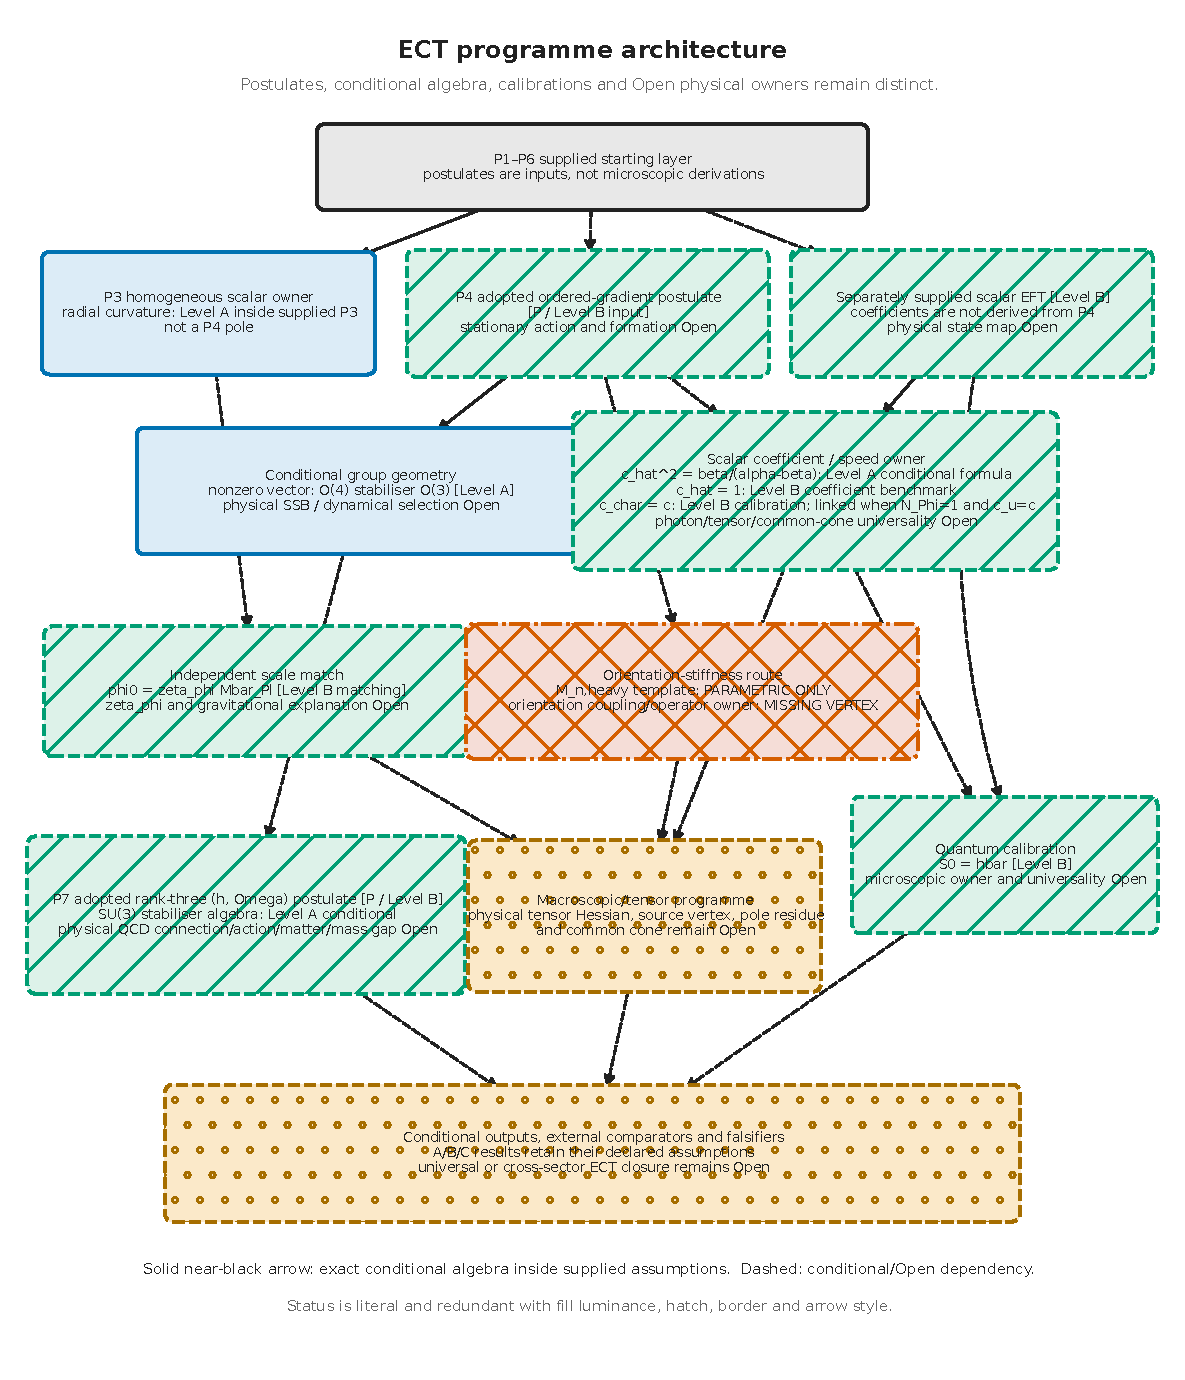
\includegraphics[width=\textwidth,height=0.70\textheight,keepaspectratio]{../figures/r177/global/fig_ect_architecture_r177.pdf}
\caption{Architectural dependency map for the minimal P1--P6 scalar sector. P4 supplies a nonzero vector datum with stabiliser $O(3)$; within the declared local algebraic scalar-operator inventory, residual symmetry fixes the two-tensor basis but not its coefficients. The displayed downstream geometric and coherent branches are conditional programmes, not simultaneous Level-A consequences: physical SSB and branch formation, the realised coefficient sign, physical clock/metric/common cones, gauge/tensor sectors and record dynamics retain their individual B/Open owners.}
\label{fig:pop_architecture}
\end{figure}

\noindent\textit{Readability note.} This portrait figure is the reader-scale map.  Its colours are redundant with literal status text and border/edge style; no arrow upgrades a node.

Spontaneous symmetry breaking (SSB) is one of the most powerful organising principles in physics. A spherical magnet has no preferred direction, until it cools below the Curie temperature and all spins align. A perfectly round ball on the tip of a Mexican hat has no preferred position, until it rolls down and selects one valley. In both cases, the underlying laws are symmetric, but the realised state is not.  These are analogies for a possible completion of P4, not a derivation of such an event in ECT.

P4 adopts a physically relevant nonzero vector datum whose stabiliser in $O(4)$ is exactly $O(3)$ (Fig.~\ref{fig:pop_architecture}). Three transverse directions remain equivalent; one aligned coordinate ($w$) is specified as a candidate time-length direction.  The physical stationary state, spontaneous $O(4)\to O(3)$ selection and clock interpretation are separate Open maps.

The ordered-gradient chart is an organising input, not a derived transition or a derivation of all familiar physics. The bare Euclidean condensate distinguishes no time or causal cone. Once the P4 datum and independent scalar-EFT coefficients are supplied, one can classify the scalar principal tensor. A Lorentzian scalar cone requires $\beta(\beta-\alpha)<0$; on the retained $\beta>0$ component this is $\alpha>\beta>0$. Formation of the chart, realised coefficient selection, the physical clock/metric, other-sector cones, excitation spectrum and decoherence hierarchy require separate owners and remain conditional/Open.

The candidate mechanism that would have to justify this chart is
\emph{gradient condensation}.  Within the adopted one-scalar, first-derivative
inventory, $\partial_A\Phi$ is the lowest-canonical-dimension local
\emph{polar-vector} order parameter.  A nonzero scalar $\langle\Phi\rangle$
is $O(4)$-invariant, whereas a supplied nonzero
$\langle\partial_A\Phi\rangle=u_0\delta_{Aw}$ has stabiliser $O(3)$.  This is
not a uniqueness theorem for all one-scalar order parameters: a nematic
composite such as
$\langle\partial_A\Phi\partial_B\Phi
-\delta_{AB}(\partial\Phi)^2/4\rangle$ could select an unoriented axis while
$\langle\partial_A\Phi\rangle=0$, with a different target and stabiliser.  In
the present P4 notation the brackets denote the adopted coarse-grained datum,
not a state-owned vacuum expectation value.  The group kinematics is exact
conditional on that datum; it does not establish a transition, vacuum or
spontaneous selection.

The gradient field can be decomposed into an amplitude and a direction:
\begin{equation}
  \partial_A\Phi = u \cdot n_A,
  \qquad u = |\partial\Phi| \geq 0,
  \qquad n^A n_A = 1.
  \label{eq:pop_polar}
\end{equation}
In the supplied ordered-sector chart, $\langle u \rangle = u_0$ and $\langle n^A \rangle = \delta^A{}_w$. This decomposition organises the conditional EFT; its physical state and selection remain Open. Each component plays a distinct role:

The \textbf{amplitude sector} contains the homogeneous P3 radial coordinate
with $m_{\Phi,{\rm rad}}^2=2\mu^2$ (Level~A inside P3).  A heavy,
short-ranged ordered-branch pole is only an OP-grad/F7 benchmark closure.
Its stationary P4 action, Hessian, pole, correlation length, gravitational
coupling and matching to the P3 coordinate remain Open; no independent
Planck-length theorem is used.

The \textbf{orientation sector} ($\delta n^A$): the abstract orbit of the
supplied nonzero vector, $O(4)/O(3) \simeq S^3$, admits three director
coordinates.  Its identification with a physical vacuum manifold is Open. On a smooth
patch of the strict scalar-only exact pullback, integrability locally
parametrises the linear soft variation by one scalar coordinate~$\chi$
(Level-A conditional kinematics).  This coordinate count does not by itself
prove that $\chi$ is a propagating physical mode or exclude scalar modes in
other completion sectors.  A one-mode physical interpretation additionally
requires a supplied reduced action, complete constraint/boundary quotient and
physical projector (Level~B); the scalar count of the completed theory remains
Open.  At fixed $\alpha,\beta$, about homogeneous $\bar n=w$, and to first
order in a tangent director perturbation, the fixed image has no linear
TT/static-density seed: $h_{ij}^{\rm TT}=h_{ww}=0$.  This is not a physical
graviton, while quadratic, nonlinear, composite, nonlocal, additional-field
and dynamical-parameter routes remain parametric/Open.  A physical spin-2
Hessian, vertex, TT projector and canonical normalisation remain Open.

The \textbf{phase mode} ($\theta$, in the coherent sector $\Phi_{\rm eff} = \rho\,e^{i\theta}$): connected to gauge fields and quantum dynamics.

The dynamical origin of gradient condensation from the bare action P3 is an
Open theoretical programme (OP-grad in the preprint).  A general local
first-derivative scalar density may depend on both $\Phi$ and
$X=(\partial_A\Phi)^2$ through $F(\Phi,X)$ and need not split as
$P(X)+V(\Phi)$.  Inside the restricted separable inventory, a pure-gradient
action $\int P(X)$ can admit an affine stationary family when
$P_X(u_*^2)=0$; this is a conditional toy route.  Once the P3 potential
$V(\Phi)$ is retained, an affine nonconstant profile also requires
$V'(u\!\cdot\!X+\Phi_c)=0$ pointwise and is not a stationary solution of the
displayed quartic P3 model.  Thus neither restricted route owns the physical
P4 state.  Given the adopted P4 chart, conditional EFT calculations can
nevertheless be organised.  Recent sharpening in the preprint decomposes
this programme into three recorded subproblems (OP3.1a--c) and localises the
remaining OP3.1a gap to a single constraint-relaxation/coarse-graining bridge:
the candidate shortcut bridges --- the EFT-level orientation route in the
strict integrable regime and the potential-sector route --- have been computed
and excluded as completions.

An important restricted result (the ``$P(X)$ no-orientation theorem'' in the preprint) concerns the strict homogeneous scalar-gradient seed: its two-derivative Hessian does not supply an independent transverse orientation stiffness. This is an A-math statement under those assumptions, not a theorem about every $P(X)$ completion, constrained reduction, inhomogeneous background, extra field, or higher-gradient operator. A physical orientation stiffness may arise only after such additional owners are specified. A covariant $S_n[g,n,\lambda_n]$, its constraints, and its metric variation are still required before a physical orientation stress or gravitational source is obtained (Open).


\section{Conditional Lorentzian classification in the supplied scalar branch}
\label{sec:pop_lorentzian}

Once the P4 vector datum is supplied, residual $O(3)$ symmetry fixes only the local algebraic two-tensor basis $\{\delta^{AB},n^An^B\}$ within the declared scalar-operator inventory.  The coefficients $\alpha,\beta$, their realised domain and the physical action owner are independent inputs.  The object that owns the displayed principal polynomial is the dimensionless characteristic quadratic form, not yet a physical action:
\begin{align}
  \mathcal Q_{2,\varphi}
  &= \frac12\int d^4X\left[
     K^{AB}\partial_A\varphi\partial_B\varphi
     +m_{\rm eff}^2\varphi^2\right],
  \qquad K^{AB}=\beta\delta^{AB}-\alpha n^An^B,
  \label{eq:pop_eft}\\
  \mathcal I_{L,\varphi}^{(2)}
  &=\varsigma_L\mathcal Q_{2,\varphi},
  \qquad
  S_{L,\varphi}^{{(2)},\rm phys}
  =A_{L,\varphi}\mathcal I_{L,\varphi}^{(2)},
  \qquad A_{L,\varphi}>0 .
\end{align}
Here $A_{L,\varphi}$ is a finite, positive, spacetime- and field-independent action scale on the displayed quadratic patch.  It is independent of the cone and is not identified with $S_0$, $\hbar$ or another sector's normalisation.  Writing $\Delta=\alpha-\beta$, the full Lorentzian domain is $\beta\Delta>0$, equivalently $\beta(\beta-\alpha)<0$.  Positive quadratic kinetic and gradient energy fixes $\varsigma_L=-\operatorname{sgn}\beta$.  This companion retains $\beta>0$, $\Delta>0$ and hence $\varsigma_L=-1$ for its explicit mostly-plus formulas.  This sign and Legendre algebra are Level-A mathematics inside the supplied quadratic model; derivation of the realised component, relative sector sign and $A_{L,\varphi}$ from P1--P6 remains Open.

This tensor has eigenvalues $\beta$ (triply degenerate, perpendicular to
$n^A$) and $\beta-\alpha$ (along $n^A$).  On the full real coefficient
plane the exact classification is
\[
 \begin{array}{ccl}
 \beta(\beta-\alpha)>0 &:& \text{nondegenerate elliptic},\\
 \beta(\beta-\alpha)<0 &:& \text{Lorentzian/hyperbolic},\\
 \beta=0\ \text{or}\ \alpha=\beta &:& \text{degenerate}.
 \end{array}
\]
For the rest of this companion, shorthand ``$\alpha>\beta$ Lorentzian
window'' means only the retained component with
$\beta>0$ and hence $\alpha>\beta>0$.  In that component the principal tensor
has signature $(-,+,+,+)$ and a scalar characteristic cone; identifying it
with the physical metric and the cones of matter, photons and tensors remains
Open.  The pair $(\alpha,\beta)=(2,1)$ is a canonical supplied benchmark,
not a vacuum-selection theorem. P4/SSB does not determine the realised
coefficient region; physical branch selection remains Open/matched.

The dimensionless common-length slope is:
\begin{equation}
  \hat c_* = \sqrt{\frac{\beta}{\alpha - \beta}},
  \label{eq:pop_cstar}
\end{equation}

The dimensional notation is fixed as follows.  The ordered Euclidean
coordinate is the \emph{time-length} $x^0\equiv w$, not an SI time.
Along an ordered worldline the physical proper time is defined by
\begin{equation}
  d\tau=\frac{\mathcal N_\Phi\,dx^0}{c_{\rm u}},
  \label{eq:pop_proper_time}
\end{equation}
Only for an aligned planar branch with constant unit lapse
$\mathcal N_\Phi=1$ and $c_{\rm u}=c$ may one use the shorthand
$t=\tau=w/c$.  The unit-slope coefficient benchmark $\hat c_*=1$ is a
Level-B unit-slope choice, not a field-rescaling identity.  In the general
relation it and the scalar-clock target have distinct owners, and a different
clock/conversion map can calibrate $c_{\rm char}=c$ at another supplied slope.
On the particular slice $\mathcal N_\Phi=1$, $c_{\rm u}=c$, however, they are
algebraically linked: $c_{\rm char}=c$ if and only if $\hat c_*=1$.  In general
$c_{\rm char}=c_{\rm u}\hat c_*/\mathcal N_\Phi$; a time variable is never
equated directly to the length coordinate.  After the clock/lapse convention
is fixed, ECT adopts $c_{\rm char}=c$ as the Level-B scalar-clock
calibration.  This does not identify the photon, matter or tensor cones, whose
kinetic owners and common-cone map remain Open.

\textbf{The strict result is a conditional signature classification, not dynamical sign selection.} Within the stated local algebraic scalar-operator inventory, residual symmetry fixes the tensor basis, and the exact full-domain condition $\beta(\beta-\alpha)<0$ gives one sign opposite to the other three.  On the retained component this is $\alpha>\beta>0$. P4 fixes neither the coefficients nor this region, the physical clock, metric, photon/matter/tensor cones or a realised vacuum. The classification is A-math conditional; physical branch selection remains Open.

\textbf{Comparison with other theories.} In Einstein--aether theory (Jacobson, 2004), the anisotropy is introduced by a vector field; Ho\v{r}ava--Lifshitz gravity breaks Lorentz invariance explicitly; CDT imposes Lorentzian causal structure on the lattice; and the Hartle--Hawking Euclidean arena is a construction for a wave function.  ECT instead studies a P4-supplied ordered scalar-gradient branch whose quadratic scalar operator has Lorentzian signature in a declared coefficient window.  That scalar statement is exact inside the supplied EFT; a physical observable metric and the photon, matter and tensor cones remain Open.

\FloatBarrier

\section{Conditional equation inventory: Euclidean scalar problem, KG form, and supplied Schr\"odinger sector}
\label{sec:pop_hierarchy}

\begin{figure}[H]
\centering
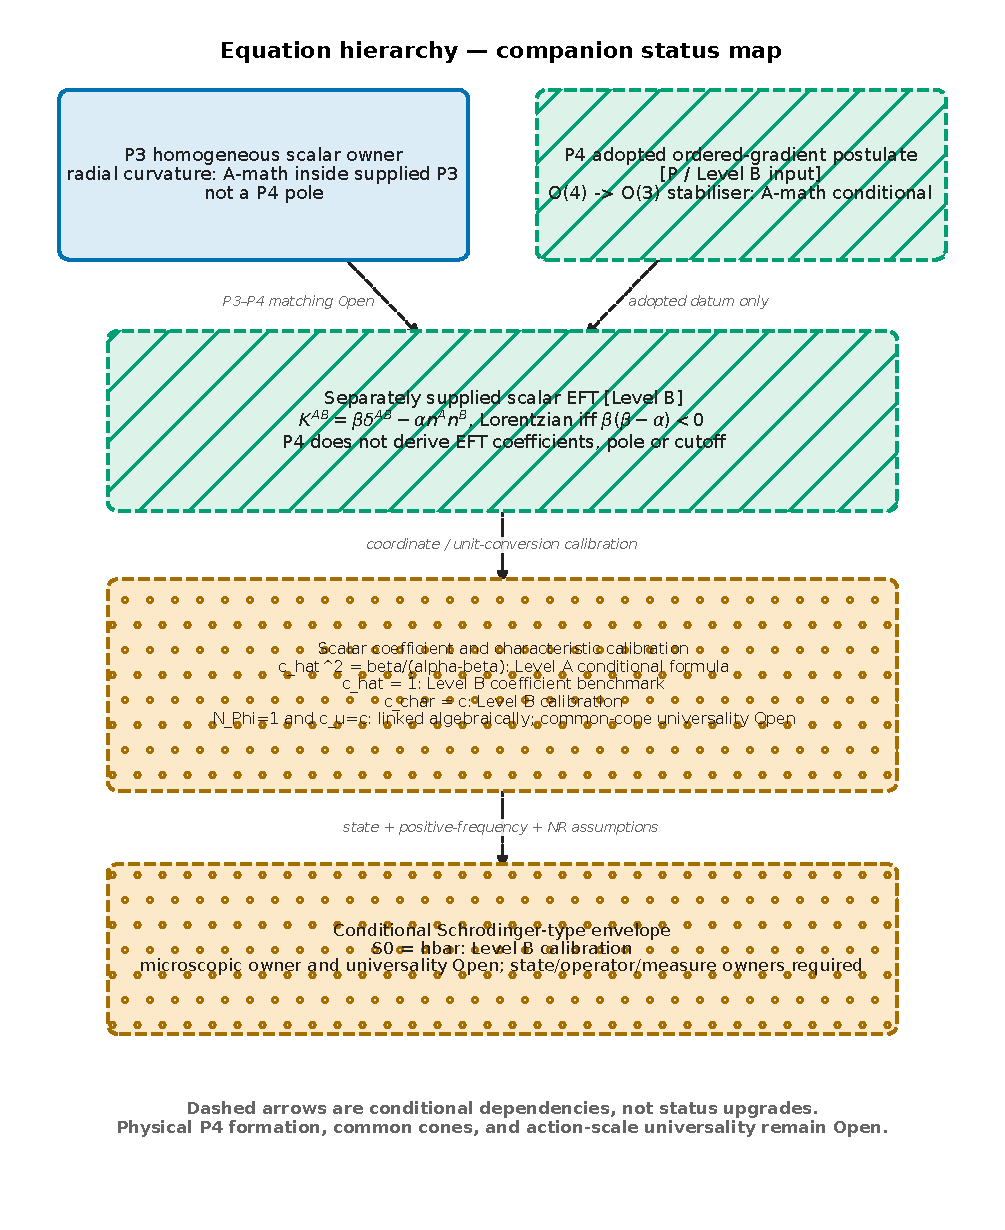
\includegraphics[width=0.96\textwidth,height=0.72\textheight,keepaspectratio]{../figures/r149/r149_equation_hierarchy.pdf}
\caption{Status-separated equation inventory. Level~0 is the bare Euclidean scalar boundary problem; Level~1 is the supplied ordered-branch scalar equation; Level~2 is its local constant-lapse Klein--Gordon form after the clock map; and Level~3 is only a leading non-relativistic Schr\"odinger envelope after a norm-preserving complex law, Hamiltonian/domain, state and positive-frequency branch, weak interaction, slow-envelope regime, physical clock and $S_0=\hbar$ calibration are separately supplied.  The shorthand $t=\tau=w/c$ additionally requires an aligned planar patch with $\mathcal N_\Phi=1$ and $c_{\rm u}=c$.  The separate $\hat c_*$ choice fixes only the scalar common-length slope.  Arrows organise conditional reductions and never upgrade the literal status written in a node.}
\label{fig:pop_hierarchy}
\end{figure}

The conditional Lorentzian classification has a direct consequence for the supplied scalar equations (Fig.~\ref{fig:pop_hierarchy}). The Euclidean field equation $\delta^{AB}\partial_A\partial_B\Phi - V'(\Phi) = 0$ is a four-dimensional \emph{boundary-value problem}: boundary data specify that problem, but fix a unique solution only after existence, uniqueness and stability/well-posedness are proved for the stated nonlinear equation, domain and boundary class. Those global properties remain Open.

On an aligned locally homogeneous, frozen-coefficient constant-lapse patch, once the ordered branch and clock map are supplied, the scalar equation has the \emph{Klein--Gordon form} $\partial_\tau^2\varphi-c_{\rm char}^2\nabla^2\varphi+M_{\rm eff}^2\varphi=0$.  The common-length and physical-clock gap coefficients are related by
\[
 \widehat M_{\rm eff}^2=\frac{m_{\rm eff}^2}{\alpha-\beta},
 \qquad
 M_{\rm eff}^2=\frac{c_{\rm u}^2}{\mathcal N_\Phi^2}\widehat M_{\rm eff}^2
 =\frac{m_{\rm eff}^2c_{\rm char}^2}{\beta}.
\]
Here $M_{\rm eff}$ is a physical-clock frequency/gap coefficient (with units of inverse time), not by itself a physical mass.  Only after the standard relativistic matter interpretation, the same physical clock and an action unit $\hbar$ are supplied may one define a mass $m$ by $M_{\rm eff}=m c_{\rm char}^2/\hbar$; neither the cone nor the clock map derives that matching.  The symbol $t$ may replace $\tau$; $t=w/c$ only in the canonical special case stated above.  If the lapse or coefficients vary, additional derivative terms occur and the displayed constant-coefficient Klein--Gordon equation is only the local frozen-patch form.

After a norm-preserving complex evolution law, Hamiltonian and domain, state space, boundary/positive-frequency branch, the physical mass matching $M_{\rm eff}=m c_{\rm char}^2/\hbar$, and a weak interaction whose supplied leading envelope is $V$ are separately admitted, write the complexified positive-frequency component as $\varphi_+=e^{-imc_{\rm char}^2t/\hbar}\psi$ (with a real field reconstructed from the paired frequency components when applicable).  In the slow-envelope regime
\[
 \epsilon_t=\frac{\hbar\|\partial_t\psi\|}{mc_{\rm char}^2\|\psi\|}\ll1,
 \qquad
 \epsilon_p=\frac{\hbar\|\nabla\psi\|}{mc_{\rm char}\|\psi\|}\ll1,
 \qquad
 \epsilon_V=\frac{\|V\|}{mc_{\rm char}^2}\ll1,
\]
and after the second envelope-time derivative and interaction-specific relativistic corrections are consistently neglected, the leading equation is $i\hbar\,\partial_t\psi = -\frac{\hbar^2}{2m}\nabla^2\psi + V\psi$.  This is Level-A asymptotic mathematics conditional on all stated inputs and a controlled residual, not an exact equality of the original equations; a quantitative error bound requires the supplied interaction owner and regularity/domain estimates.  ECT ownership of those inputs remains Level-B/Open, while $S_0=\hbar$ is a separate Level-B empirical calibration.

This is a status-separated inventory rather than a generic descent theorem.  The real phase action or Euclidean boundary-value problem alone derives neither the norm-preserving complex law nor its state, Hamiltonian, interaction and positive-frequency sector.  Identification with the textbook Schr\"odinger equation, its physical states, controlled approximation domain and Born/detector map therefore remains Level-B/Open rather than a completed derivation from P1--P6.

The Euclidean formulation is a boundary-value problem rather than a Lorentzian Cauchy problem. This mathematical distinction is structural; its mapping to entanglement, delayed-choice settings, and laboratory probabilities remains B/Open and requires a physical state, boundary map, and measurement kernel.

\FloatBarrier

\section{Causal cone inheritance and what GW170817 tells us}
\label{sec:pop_cone}

A critical question for any emergent-spacetime theory is whether its separately specified candidate physical sectors share the observed relativistic cone.  The supplied scalar model conditionally defines one characteristic cone, but this fact alone cannot assign the principal symbols of photons or gravitational waves.  Cone universality is therefore a cross-sector completion test, not a theorem obtained merely from the existence of one condensate.

In August 2017, the LIGO/Virgo gravitational-wave detectors observed the neutron-star merger \textbf{GW170817}; Fermi and INTEGRAL detected the associated gamma-ray burst about 1.7 seconds later after a journey of roughly 130 million light-years~\cite{LIGO_Virgo_GW170817_2017}.  Under the standard source-delay assumptions, the multimessenger bound is conventionally quoted as $-3\times10^{-15}\lesssim(c_{\rm GW}-c)/c\lesssim7\times10^{-16}$.  This is an external constraint on any future physical ECT tensor completion, not a prediction of the displayed scalar/director map.

In generic Lorentz-violating or derivative-coupled completions, matching
independently owned matter and tensor cones imposes model-dependent
constraints.  The Standard Model Extension parametrises sector-dependent
Lorentz-violating coefficients.

The P4 datum supplies only the aligned director.  The scalar characteristic tensor $K^{AB}$ and its coefficients are separately supplied, while the phase sector requires three distinct quadratic owners.  On a locally homogeneous, frozen-coefficient aligned patch with $K_\theta^{\rm eff}>0$ and the retained $\beta>0$ component, define
\begin{align*}
 \mathcal I_{\theta,E}
 &=\frac{K_\theta^{\rm eff}}2\int d^4X\,
   \delta^{AB}\partial_A\theta\partial_B\theta,\\
 \widehat K^{AB}&\equiv K^{AB}/\beta,
 \qquad
 \mathcal Q_{\theta,K}
 =\frac{K_\theta^{\rm eff}}2\int d^4X\,
   \widehat K^{AB}\partial_A\theta\partial_B\theta,\\
 \mathcal I_{\theta,L}&=-\mathcal Q_{\theta,K}
 =\frac{K_\theta^{\rm eff}}2\int dx^0d^3x
 \left[\frac{(\partial_0\theta)^2}{\widehat c_*^2}
       -(\nabla\theta)^2\right].
\end{align*}
The first is a non-negative Euclidean quadratic functional whose principal operator is elliptic.  Its kernel contains functions constant on every connected component.  Positive definiteness on the admissible space requires a declared domain and boundary conditions and absence or removal of the full kernel; quotienting one constant zero mode alone is insufficient on a disconnected domain.  Coercivity in the declared norm additionally requires a positive spectral gap (a Poincar\'e inequality), which need not follow from kernel removal on a non-compact domain.  The second owns the characteristic polynomial, and the third is the positive-energy Lorentzian reduced action.  A physical phase action requires $S_{\theta,L}^{\rm phys}=\Sigma_\theta\mathcal I_{\theta,L}$ with finite positive, spacetime- and field-independent constant $\Sigma_\theta$; using the same $\Sigma_\theta$ in a Euclidean weight is an additional same-sector matching input.  Unspecified higher operators and variable-coefficient terms are not included in this displayed quadratic truncation.  Consequently the status-separated cone inventory is
\begin{equation}
  \begin{aligned}
  c_{\rm phase}&=c_{\rm char}
    &&\text{only in this supplied phase truncation after the same clock/lapse map},\\
  c_\gamma&\stackrel{?}{=}c_{\rm char},
    &c_{\rm GW}&\ \text{Open}.
  \end{aligned}
  \label{eq:pop_cone}
\end{equation}
A shared $K^{AB}$ fixes only the common-length slope; equality of physical speeds additionally requires the same supplied physical clock/lapse map.  A photon cone can coincide with it only after the Abelian gauge owner and kinetic normalisation are established; a GW cone requires a physical constrained tensor Hessian.  The displayed phase algebra is Level-A mathematics conditional on the supplied quadratic owners, while the action magnitude, common physical clock, their derivation and cross-sector universality remain Level-B/Open inputs.
GW170817 is an external kill gate for a future ECT tensor completion.  The current scalar characteristic cone does not identify the gravitational-wave cone.

Higher-derivative dispersion and sector-dependent corrections can be assessed only after each physical kinetic owner is supplied.  Any completed ECT sector must satisfy the corresponding laboratory and multimessenger cone bounds; the current scalar result neither forbids nor predicts an unsuppressed tensor-sector difference.


\section{Two energy scales and a separate galactic length}
\label{sec:pop_scales}

\begin{figure}[H]
\centering
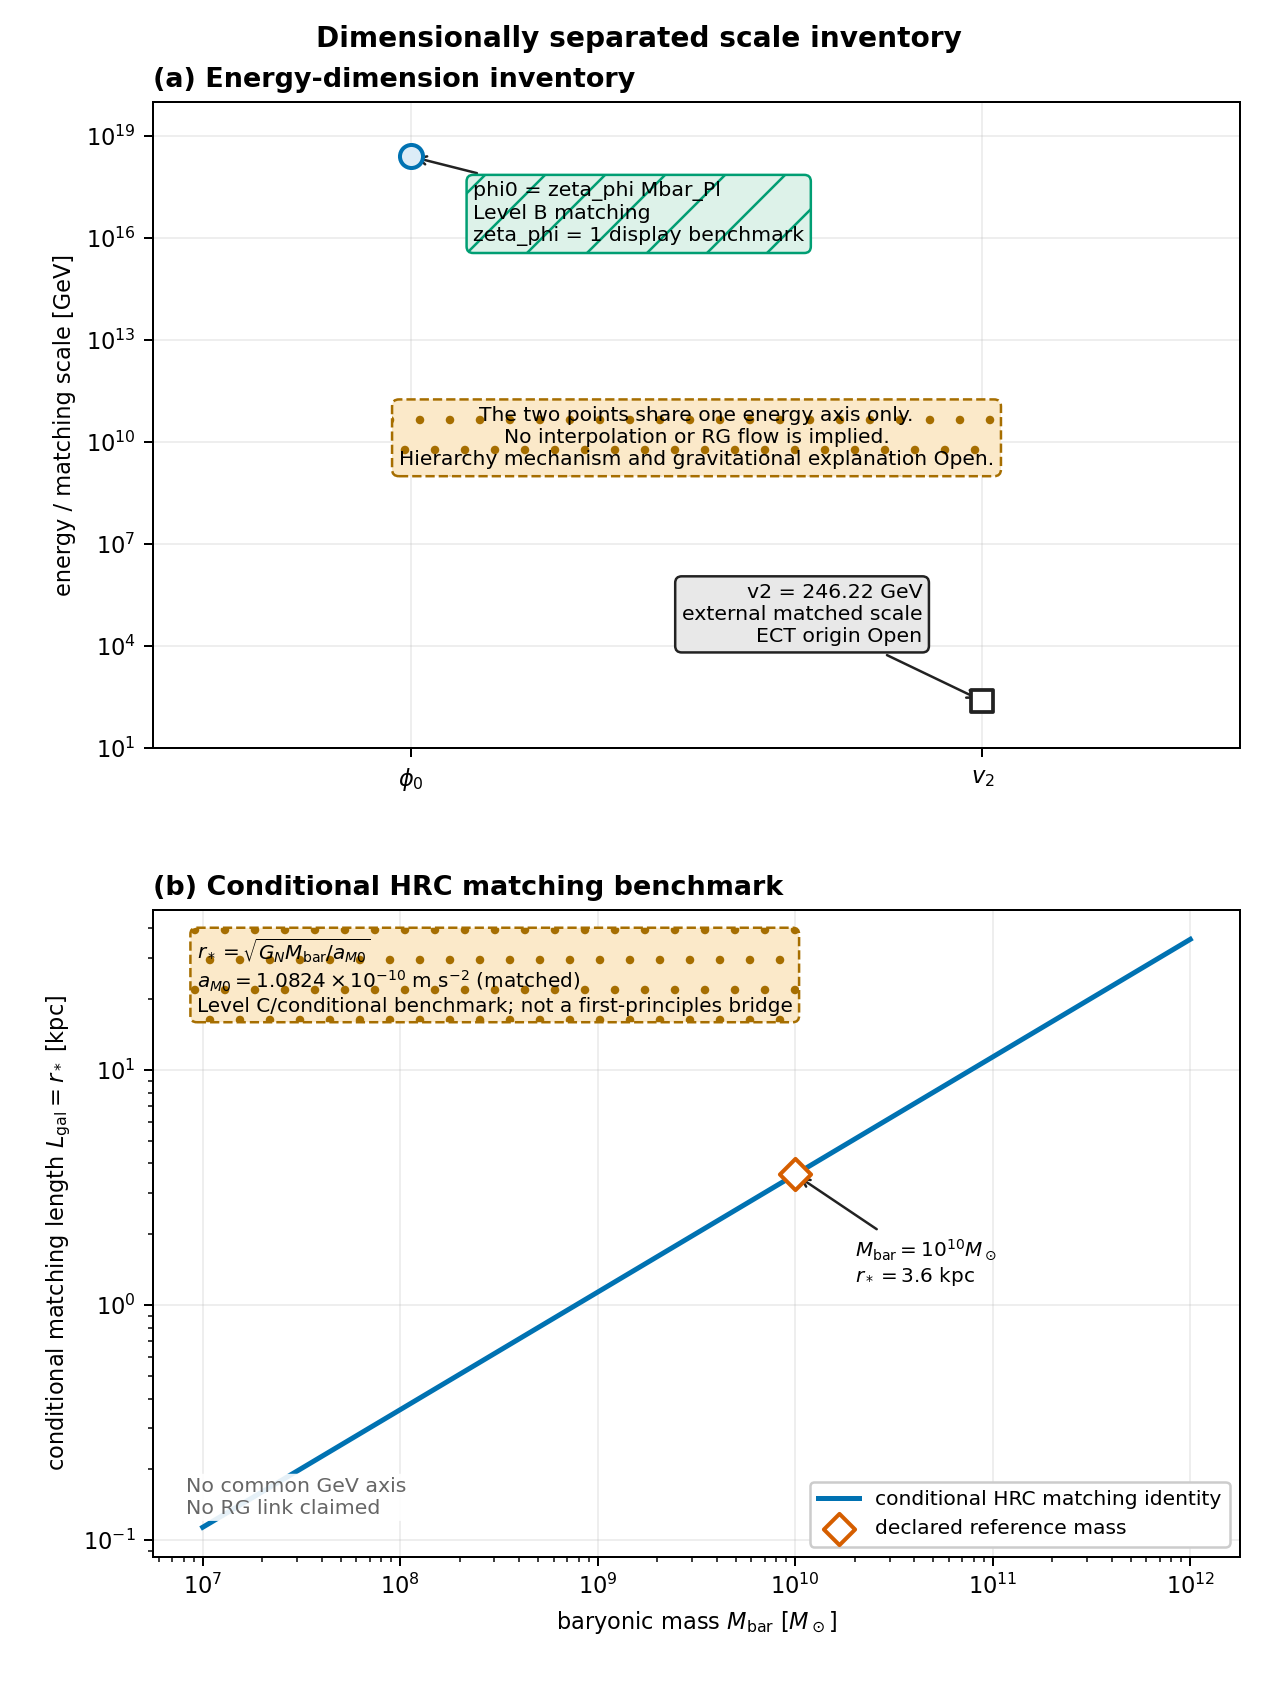
\includegraphics[width=0.92\textwidth]{../figures/r153/line_semantics/fig_condensate_scales_line_semantics_r153.png}
\caption{Dimensionally separated scale inventory.  The left panel compares the two energy-dimension quantities $\phi_0$ and $v_2$; they are independent inventory points, so no connecting curve or interpolation is implied.  The gradient amplitude $u_0$ has units GeV$^2$ and is related only by the conditional dimensional estimate $u_0\sim\phi_0m_\sigma$.  The right panel shows the distinct length $L_{\rm gal}=r_*=\sqrt{G_NM_{\rm bar}/a_M}$ inside the conditional HRC gravity functional.  No common-axis RG flow or first-principles bridge among these objects is claimed.}
\label{fig:pop_scales}
\end{figure}

The current inventory contains two quantities with energy dimension,
$\phi_0$ and $v_2$, plus the dimension-two gradient amplitude $u_0$ and
the separate Level-C galactic length $L_{\rm gal}$
(Fig.~\ref{fig:pop_scales}).  They must not be plotted on one energy
axis or described as three amplitudes generated by one RG mechanism.

The \textbf{Planck-like energy scale} is an independent matching input.  ECT
adopts
\begin{equation}
  \phi_0=\zeta_\phi\bar M_{\rm Pl},
  \qquad \zeta_\phi>0,\quad \zeta_\phi=O(1),
\end{equation}
as a Level-B scale ansatz; the canonical benchmark $\zeta_\phi=1$ gives
$\phi_0\simeq2.435\times10^{18}$\,GeV.  The controlled matching inventory is
\begin{equation}
  G_N^{\rm nat}=\frac{1}{8\pi M_G^2},\qquad
  S_0=\hbar\ \text{(adopted calibration)},\qquad
  c_{\rm char}=\frac{c_{\rm u}\hat c_*}{\mathcal N_\Phi},\qquad
  \hat c_*^2=\frac{\beta}{\alpha-\beta}.
  \label{eq:pop_matching}
\end{equation}
The displayed Open bridge from ordered-sector stiffness to $M_G$ contains no
$\phi_0$ and therefore does not derive the scale ansatz.  The gradient
amplitude instead has $[u_0]={\rm GeV}^2$ and only the dimensional estimate
$u_0\sim\phi_0m_\sigma$; its value is not a third energy scale.

The \textbf{electroweak energy scale} $v_2\simeq246$\,GeV is a
matched secondary scale.  The logarithm
$\mathcal I_{\rm EW}=\ln(\phi_0/v_2)\approx36.8$ for the displayed
matched scales and organises an Open non-polynomial scale-generation
programme.  This arithmetic ratio is not a derived naturalness mechanism;
none of the candidate mechanisms has been derived from P1--P6.

The \textbf{galactic length}
$L_{\rm gal}=r_*=\sqrt{G_NM_{\rm bar}/a_M}$ is conditional on
baryonic mass and the fitted acceleration $a_M$ inside the
adopted Level-C functional.  For $M_{\rm bar}=10^{10}M_\odot$ and
$a_{M0}=1.08\times10^{-10}$\,m/s$^2$, it is about
$3.4$--$3.7$\,kpc.  Its scalar/ECT origin and environment law remain
Open.

No additional energy scale is selected from $(\phi_0,v_2)$ by dimensional
analysis alone: infinitely many composite functions have the required
dimension.  ECT adopts the Level-B programme hypothesis that the P3/P4,
electroweak, infrared and HRC scales should admit a common-medium matching in a
completed theory, but no present relation among $\phi_0$, $u_0$, $v_2$, $a_M$
and $m_\chi$ follows without a separate named closure.  In particular, the
existence, action and dynamics of a proposed second ordering step remain Open.
Higher-dimension Yukawa corrections are organized as powers of
$v_2/M_{Y,\mathrm{heavy}}$ for a separately supplied
$M_{Y,\mathrm{heavy}}>0$; only the additional named match
$M_{Y,\mathrm{heavy}}=c_Y\phi_0$, $c_Y>0$, turns this into powers of
$v_2/(c_Y\phi_0)$.  No equality to the orientation or neutrino heavy scale is
implied.  A neutrino or other application therefore
requires its own operator, coefficient, flavour/state content and matching
map.

\FloatBarrier

\section{Compact-phase winding and the conditional cohesive-defect loop programme}
\label{sec:pop_loops}

The compact phase gives a Level-A existence result for integer winding
sectors inside its declared closure.  Turning those sectors into a localised
carrier, a distinguished physical action scale, quantum interference, or a
complete discrete spectrum requires additional dynamics and matching.

In the coherent sector, the effective order parameter has the polar form
$\Phi_{\rm eff}=\rho e^{i\theta}$, with $\rho>0$ along the contour under
discussion.  Single-valuedness applies to $\Phi_{\rm eff}$, not to a globally
single-valued real lift of $\theta$: on a closed contour $\mathcal C$ that
does not intersect a defect core, $\Phi_{\rm eff}$ defines a map
$\mathcal C\to S^1$.  A locally lifted phase therefore obeys
\begin{equation}
  \oint_{\mathcal{C}} \partial_A\theta\,dX^A = 2\pi n,
  \qquad n \in \mathbb{Z}.
  \label{eq:pop_winding}
\end{equation}
The integer is the degree of that map.  This is not a quantum axiom; it is an
exact topological statement only inside the supplied non-vanishing
compact-phase closure.  A contour crossing $\rho=0$, or a homotopy allowed
to pass through such a zero, lies outside that protected sector and can
permit unwinding.

Inside the older phase-only fixed-core closure, the corresponding reduced
elementary loop coefficient is
\begin{equation}
  \iota_{\rm elem}^{\rm(fixed\ core)}
  =2\pi\iota_0^{\rm EFT},
  \label{eq:pop_Sloop}
\end{equation}
and the physical action would be
$S_{\rm elem}^{\rm phys}=\Sigma_\theta
\iota_{\rm elem}^{\rm(fixed\ core)}$.  The dimensionless
$\iota_0^{\rm EFT}$ is supplied only after a loop length, transverse profile
and reduced normalisation are admitted; $\Sigma_\theta$ requires its own
four-dimensional owner.  Compactness supplies the integer, not a finite
nonzero global minimum: the phase-only reduced contribution falls as $1/L$
when the length is allowed to grow.  Neither the product's value nor
cross-sector ownership is derived, and only
$\Sigma_\theta\iota_0^{\rm EFT}$ may be mapped to $S_0$ and then separately
calibrated to~$\hbar$.

\paragraph{Post-order candidate constitutive hypothesis CDE-$\Phi$.}
``Cohesive defect elasticity'' is a simple acceptance criterion for a
completed ordered-branch EFT: at least one stationary localised disturbance
must heal to the ambient state, have finite positive vacuum-subtracted
action per proper carrier length, and have a positive projected metric on
every retained physical normalisable modulus.  In plain language, extending
the disturbance and changing a genuine internal coordinate must both cost
positive action.  CDE-$\Phi$ is not a pre-physical property, a new frozen
postulate, or the owner of the equations.  It supplies neither gravity nor
quantisation, and it does not manufacture a compact modulus.

The actual owner must be one explicit four-dimensional completion action
together with its state and boundary data, a stationary profile, a fixed
vacuum subtraction and regulator, and the constraint/gauge/frame/zero-mode
quotient used to define physical fluctuations.  Suppose that owner supplies
completion fields $\Psi^I$, a localised profile
$\Psi_*^I(y;\vartheta)$ around a one-dimensional Euclidean carrier
$X^A(s)$, and a genuine compact normalisable modulus
$\vartheta\sim\vartheta+2\pi$.  A controlled collective-coordinate
reduction~\cite{Manton1982Moduli} can then take the schematic form
\begin{equation}
 S_{E}^{\rm sub,phys}=\Sigma_\vartheta\mathcal I_E^{\rm sub},
 \qquad
 \mathcal I_E^{\rm sub}=\int ds\left[
 \mathcal T_{\rm loop}
 +\frac{K_\vartheta^{1\mathrm D}}{2}(D_s\vartheta)^2
 +\frac{\kappa_b}{2}\mathcal K^2+\cdots\right].
 \label{eq:pop_cde_reduction}
\end{equation}
Here $\mathcal K$ is carrier curvature and $D_s$ includes any derived
connection.  Twist, torsion, mixed curvature--modulus, nonlocal and
higher-derivative terms hidden in the ellipsis must be retained whenever
the owner allows them.  Before constrained profile relaxation,
\begin{equation}
 \mathcal T_{\rm loop}
 =\frac{1}{\Sigma_\vartheta}\int d^3y\,
 [\mathcal L_E(\Psi_*)-\mathcal L_E(\Psi_{\rm vac})],
 \qquad
 K_\vartheta^{1\mathrm D}
 =\frac{1}{\Sigma_\vartheta}\int d^3y\,G_{IJ}\,
 \partial_\vartheta\Psi_*^I\partial_\vartheta\Psi_*^J .
 \label{eq:pop_cde_coefficients}
\end{equation}
with the state, boundary data, regulator and quotient understood.  The
reduced modulus metric is the corresponding constrained Schur
complement, not an unconstrained positive-looking integral; the physical
action-valued coefficient is $\Sigma_\vartheta K_\vartheta^{1\mathrm D}$.  These formulas are a
derivation template, not evidence that the minimal real-scalar P3 action has
the required carrier or compact modulus.

The best-matched ECT-native owner candidate is a stabilised
three-dimensional orientation texture whose worldline carries an
independently established compact normalisable modulus.  This remains Open:
a static two-derivative texture has the usual Derrick-collapse obstruction,
the exact-gradient branch can restrict the orientation image to a
contractible hemisphere, and no required stabilising higher-gradient or
independent-orientation completion has been derived from P1--P6.

The transverse $d^3y$ measure describes a codimension-three curve in four
Euclidean dimensions.  Thus $L=\int_\Gamma ds$ is worldline proper length or
Euclidean period, not the spatial radius of a texture.  A spatial vortex loop
persisting along the selected direction would instead trace a
codimension-two worldsheet and requires a different reduction.  A
reparametrisation-invariant worldline representative makes the ensemble
condition precise.  For $\tau\in[0,1]$, einbein $e(\tau)>0$,
$L=\int_0^1e\,d\tau$ and
$\vartheta(1)-\vartheta(0)=2\pi n$,
\begin{equation}
 S_{\rm wl}^{\rm phys}[e,\vartheta]
 =\Sigma_\vartheta\mathcal I_{\rm wl}[e,\vartheta],
 \qquad
 \mathcal I_{\rm wl}[e,\vartheta]
 =\int_0^1d\tau\left[
 \mathcal T_{\rm loop}e+
 \frac{K_\vartheta^{1\mathrm D}}{2e}\dot\vartheta^2\right].
 \label{eq:pop_balanced_loop}
\end{equation}
For the following bending-free minimum, assume
$K_\vartheta^{1\mathrm D}>0$, $\mathcal T_{\rm loop}>0$, $L>0$ and
$n\ne0$.  The $\vartheta$ equation then gives
$K_\vartheta^{1\mathrm D}\dot\vartheta/e=\mathrm{const}$ and hence
$\dot\vartheta=2\pi n e/L$.  Substitution produces
\begin{equation}
 \mathcal I_n^{(\vartheta)}(L)=\mathcal T_{\rm loop}L+
 \frac{2\pi^2K_\vartheta^{1\mathrm D}n^2}{L},
\qquad
 L_{*,n}=\pi|n|\sqrt{\frac{2K_\vartheta^{1\mathrm D}}
                                  {\mathcal T_{\rm loop}}},
\qquad
 \mathcal I_{n,\min}=2\pi|n|\sqrt{
 2K_\vartheta^{1\mathrm D}\mathcal T_{\rm loop}} .
 \label{eq:pop_balanced_min}
\end{equation}
The modulus route defines the distinct coefficient
\begin{equation}
 \iota_{0,\rm bal}^{(\vartheta)}
 =\sqrt{2K_\vartheta^{1\mathrm D}\mathcal T_{\rm loop}},
\qquad
 \iota_{0,\rm bal}^{(\vartheta)}=\iota_{0,\rm bal}^{\rm eff}
 \ \text{only after that owner map}.
 \label{eq:pop_balanced_relation}
\end{equation}
For the bending-free elementary branch, the physically motivated matching
chain may then be stated without conflating matching with derivation:
\begin{equation}
 \iota_{0,\rm bal}^{(\vartheta)}
 =\frac{\mathcal I_{1,\min}}{2\pi},\qquad
 \Sigma_\vartheta\iota_{0,\rm bal}^{(\vartheta)}
 \xrightarrow{\ \mathcal M_{\rm bal}\ }S_0
 \mathrel{\overset{\mathcal M_\hbar}{\longleftrightarrow}}\hbar
 \quad\Longrightarrow\quad
 \Sigma_\vartheta\mathcal I_{1,\min}=2\pi\hbar=h_{\rm P},
 \qquad
 2K_\vartheta^{1\mathrm D}\mathcal T_{\rm loop}=(\hbar/\Sigma_\vartheta)^2 .
 \label{eq:pop_planck_matching_conditional}
\end{equation}
The first equality is exact in the supplied T1 model.  The arrow
$\Sigma_\vartheta\iota_{0,\rm bal}^{(\vartheta)}\to S_0$ is an Open
candidate-to-operational owner map.  The final equality $S_0=\hbar$ is the
separately adopted Level-B physical calibration.  Conditional on both steps,
$h_{\rm P}$ is the calibrated elementary-loop physical action and $\hbar$ is
the calibrated product
$\Sigma_\vartheta\iota_{0,\rm bal}^{(\vartheta)}$, not a dimensionless reduced
coefficient.  Neither the candidate owner map, $\Sigma_\vartheta$, the
calibration's microscopic explanation nor its cross-sector universality is
derived from P1--P6 or T1.

The algebra is Level~A inside the supplied one-coordinate model.  Its
interpretation as a physical stationary length requires the proper-time zero
mode to belong to a declared closed-worldline measure or variational
ensemble.  If the duration is externally fixed, or the einbein zero mode is
pure gauge, $L$ is not varied and the displayed minimum is not a size
prediction.  With that ensemble supplied, the optimal gradient is independent
of $|n|$, while $L_{*,n}$ and $\mathcal I_{n,\min}$ are linear in $|n|$.  This makes a
single multiwinding carrier exactly marginal against separated unit carriers
in the two-term truncation; the $n=0$ branch has no finite two-term minimum.
Neither statement is a binding or population theorem.

If the same owner gives $\kappa_b>0$, the curvature bound selects a circle at
fixed length and the conditional minimum becomes
\begin{equation}
 \mathcal I_{n,\min}^{\rm circ}
 =2\pi\sqrt{2\mathcal T_{\rm loop}
 (K_\vartheta^{1\mathrm D}n^2+\kappa_b)} .
 \label{eq:pop_bending_min}
\end{equation}
Bending therefore changes the reduced minimum and, for a fixed
$\Sigma_\vartheta$, the corresponding physical action scale; it makes the
result nonlinear in $|n|$, and removes the bare two-term splitting marginality.  It cannot be
invoked while retaining the old numerical minimum unchanged.  In the
restricted space of nonempty smooth one-component closed curves, the $n=0$
branch has
$L_{*,0}^{\rm circ}=\pi\sqrt{2\kappa_b/\mathcal T_{\rm loop}}$ and
$\mathcal I_{n=0,\min}^{\rm circ}=2\pi\sqrt{2\kappa_b\mathcal T_{\rm loop}}$.
The empty vacuum and core-fill-in paths are absent from that curve space, so
this is not a proof of a stable or metastable physical loop.  If one
identical positive per-carrier $\kappa_b$ is used and every other interaction
is omitted, the connected-circle truncation obeys
$\mathcal I_{n,\min}^{\rm circ}<n\mathcal I_{1,\min}^{\rm circ}$ for $n>1$.  This is exact
same-core subadditivity in the supplied curve model, not a physical binding
verdict: separated-core interactions, core relaxation, reconnection,
splitting and the decay barrier remain Open.  Stable Skyrme-type textures show only
that an independent orientation field with a separately supplied positive
higher-derivative operator can evade two-derivative Derrick
collapse~\cite{Skyrme1961Nonlinear}; they are external proofs of class, not
the ECT owner.

Nor does the asymptotic loop-gas count supply the missing physical
normalisation.  With coarse-graining length $b$, action denominator
$a_{\rm measure}$ and connective factor $\mu$, marginality requires
$\mathcal T_{\rm loop}b/a_{\rm measure}=\ln\mu$.  Only after independently
imposing $\mathcal I_{1,\min}/a_{\rm measure}=2\pi$ does one obtain
$L_*/b=\pi/\ln\mu=1.51$--$1.64$ for representative
$\mu=6.774$--$8$.  That circumference is shorter than two lattice steps and
therefore lies outside both the large-loop counting asymptotics and a
controlled thin-curve regime.  This is a UV-control failure of the combined
assumptions, not a derivation of $\hbar$.

A complete calculation must still derive the carrier and codimension,
compact physical modulus, common coefficients and subtraction, projected
Hessian, shape terms, topology and finite-action unwinding barrier,
splitting interactions, Lorentzian continuation, measure and cross-sector
normalisation.  Only after those gates close could one compute a physical
eigenmode spectrum, phase-slip lifetime, fragmentation diagram or
universality test.  PES-R enters only after the carrier, physical modes,
state, noise and record protocol exist; it can test admissibility,
persistence and records, but it supplies none of the missing owner data and
does not turn any candidate scale into $\hbar$.



\section{The arrow of time and the second-law programme}
\label{sec:pop_arrow}

In the Euclidean picture, the coordinate $w$ is one of four equivalent
directions.  It has no fundamental ``forward'' or ``backward'' orientation.
P4 supplies a preferred Euclidean direction.  After a supplied
$\beta(\beta-\alpha)<0$ scalar operator and a chosen initial-boundary orientation,
the scalar problem admits retarded support.  This does not identify physical
time or a thermodynamic arrow.

ECT separates three statements.  First, a supplied hyperbolic scalar operator
admits retarded support after an initial--boundary orientation is chosen.
Second, a positive pairwise noise kernel suppresses selected coherences in a
declared reduced channel.  Neither statement alone proves monotone von
Neumann entropy.

An entropy theorem additionally requires the reduced map, initial state,
entropy functional, and hypotheses such as unitality, detailed balance, or
contractivity relative to a stationary state.  Under a declared contractive
channel one may obtain
\begin{equation}
  \frac{d}{dw}D(\rho_w\Vert\rho_*)\le0,
  \label{eq:pop_2ndlaw}
\end{equation}
but this is a conditional open-system result; the ECT-specific channel and
stationary state remain Open.  Ohmicity and Markovianity alone imply no
universal scalar entropy-rate law.

Likewise, a Crooks relation requires named forward/reverse protocols, path
measures, a measurable time-reversal map $\Theta$, initial ensembles, and
local detailed balance.  The reverse measure must first be transported to
the common forward path space,
$P_R^\Theta(A):=P_R(\Theta A)$.  One-way $P_F\ll P_R^\Theta$ defines the
Radon--Nikodym entropy variable, whereas the reciprocal relation and a unit
integral fluctuation identity require $P_F\sim P_R^\Theta$; singular or
absolute irreversibility must be treated separately.  A pairwise dephasing
exponent is not this forward/reverse likelihood ratio.  The ECT
entropy-production/fluctuation-relation construction therefore remains an
explicit research programme rather than a derived second law.

\section{Spectrum, branching, gauge symmetries, and particles}
\label{sec:pop_spectrum_etc}

Decoherence exponents are channel-, state-, and protocol-dependent, and no universal forward/reverse law or single object-placement axis has been derived.

The supplied ordered-chart bookkeeping separates three candidate sectors;
their physical excitation content is owner-dependent:

\textbf{Amplitude sector:} The homogeneous P3 expansion has a radial
coordinate with $m_{\Phi,{\rm rad}}^2=2\mu^2$ (Level~A inside P3).
It does not identify a stationary P4 pole.  A physical ordered-branch
amplitude action, Hessian, pole, correlation length and matching to the P3
coordinate remain Open.

\textbf{Orientation sector ($\delta n^A$):} On a smooth strict scalar-only
pullback, integrability reduces the independent linear soft parametrisation to
one longitudinal coordinate~$\chi$ (Level-A conditional kinematics).  A
physical propagating mode requires the separately supplied reduced action,
constraint/boundary quotient and projector (Level~B/Open).  At fixed
$\alpha,\beta$, on the homogeneous $\bar n^A=\delta^A_w$ background and at
tangent-director linear order, the fixed map has no TT/static-density seed;
a massless spin-2 field is therefore an Open completion target rather than
an induced mode of that scoped map.  For a separately supplied linear scalar operator
$(-\beta\nabla^2+m_\sigma^2)\sigma=J$, $\beta>0$, the exterior of a compact
source solves the homogeneous modified-Helmholtz equation; every nonzero
exterior multipole has Yukawa exponent $m_\sigma/\sqrt\beta$, but its amplitude
may vanish.  A nonzero exterior response over a distance $L$ requires
$m_\sigma/\sqrt\beta\lesssim L^{-1}$ (Level~A inside that supplied operator).
Conversely, an extended prescribed profile can be driven, so compact-source
asymptotics are not a universal no-response theorem.  At the separately
declared point $\phi_\infty=\bar M_{\rm Pl}=2.4353\times10^{18}$\,GeV,
$\lambda=10^{-2}$ and $\beta=1$, the proxy gives
$m_\sigma=3.444\times10^{17}$\,GeV,
$\xi_\sigma=5.730\times10^{-34}$\,m and
$(m_\sigma/\sqrt\beta)/[\hbar c/(1\,\mathrm{kpc})]
=5.386\times10^{52}$.  This is only a Level-C negative control for the
named unsourced exterior pole, not a P4 identification, galactic fit or ECT
prediction.  Named C/Open soft-scalar completions may separately posit
$g_\chi(k)=c_\chi k/f_\chi$ with independent $c_\chi,f_\chi$, or
with $H_0^{(\mathrm{freq})}>0$ and
$H_{0,E}:=\hbar H_0^{(\mathrm{freq})}$, the named branch sets
$m_\chi c^2=\zeta_HH_{0,E}$ for independent $\zeta_H>0$, giving the reduced
Compton proxy $\xi_\chi=c/(\zeta_HH_0^{(\mathrm{freq})})$.  The separate
boundary choice $\zeta_H=0$ is a massless branch with $\xi_\chi=\infty$ only
as a limit; the quotient is not used there.  At the explicit orientation
point $\zeta_H=\zeta_\phi=1$,
$\phi_0=\bar M_{\rm Pl}=2.4353\times10^{18}$\,GeV and
$H_0^{(\mathrm{freq})}=70\,\mathrm{km\,s^{-1}\,Mpc^{-1}}$, the values are
$m_{\chi,E}=1.493\times10^{-33}$\,eV and
$\xi_\chi=1.322\times10^{26}$\,m, while
$m_{\chi,E}/\phi_0=6.131\times10^{-61}$.  These are Level-C scale
conversions, not a particle prediction.  Neither branch is selected by P1--P6 or fixes
abundance, dark-matter/dark-energy identity, HRC response or a laboratory
signal.  The physical P4 pole, action, state, source vertex and
gravity/observable maps remain Open.

\textbf{Phase mode ($\theta$):} In the coherent sector, the compact phase supplies winding sectors and a conditional Abelian-connection route.  A physical, unbroken photon and its coupling to matter are not yet derived.

The supplied architecture admits conditional geometric and coherent effective
descriptions, but they are not separated by a universal decoherence scalar.
Macroscopic geometry is an ordered-chart long-wavelength closure; coherence
and record formation depend on a declared subsystem/environment split, state,
and protocol.  A pairwise exponent can diagnose a reduced channel but does
not define an ontological or metric-signature transition.

\subsection{Gauge symmetries and the interaction sectors}
\label{sec:pop_gauge}

ECT does not postulate all gauge structures as independent primitive symmetries.  P5 supplies deformability and relational response, not a gauge bundle.  A physical connection exists only after the bundle, quotient by genuinely redundant internal directions (or reduced Hessian), kinetic operator, state and matter representation have been specified.  The supplied compact phase gives a \emph{conditional} Abelian route; the orientation algebra gives only a candidate weak-sector analogy.  For colour, the minimal $O(4)$ algebra admits no direct injective $\mathfrak{su}(3)$ Lie-subalgebra embedding; emergent/nonlinear, independently supplied bundle and defect-kernel routes are not excluded.  P7 is an adopted Level-B frame-module postulate; its physical-colour identification and dynamics remain C/Open/Open, and it is not a necessary or unique completion.

\textbf{Abelian gauge route (\emph{B/Open}):} The compact coherent phase $\theta\sim\theta+2\pi$ supports a candidate principal-$U(1)$ connection once local bundle covariance is admitted.  On the ordered background the leading parity-even quadratic basis contains both $F_{AB}F^{AB}$ and $(n^AF_{AB})(n_CF^{CB})$; Maxwell form is the special choice with zero coefficient for the second invariant, not a consequence of compactness, covariance or P5 alone.  The physical gauge volume and reduced Hessian, kinetic normalisation, charge operator and matter representation, and the identification with $U(1)_Y$ or an unbroken $U(1)_{\rm em}$ all remain Open.  In particular, a charged condensate can Higgs rather than preserve the candidate photon, so masslessness must be demonstrated in the completed action.

\textbf{Weak-sector programme (\emph{A algebra/Open physical}):} The residual orientation structure after $O(4)\to O(3)$ has the exact Lie-algebra identity $\mathfrak{so}(3)\cong\mathfrak{su}(2)$, and its spinorial lift can be written in $SU(2)$ language.  This algebra does not select a local internal $SU(2)_L$ bundle, physical chirality or parity violation.  Hopf-fibered phase--orientation locking is a candidate global geometry only.  Its dynamics, the maps $SU(2)_{\rm orient}\to SU(2)_L$ and $U(1)_\theta\to U(1)_Y$, local gauge fields, matter representations, couplings, and protection of the secondary radial mode all remain Open.

\textbf{Strong interaction (\emph{restricted obstruction A; physical colour Open}):} because $\dim\mathfrak{su}(3)=8>6=\dim\mathfrak{so}(4)$, $SU(3)$ colour cannot be realised as a direct injective Lie-subalgebra or residual-factor embedding in the displayed minimal $O(4)$ algebra.  The theorem excludes only that route: emergent/nonlinear constructions, independently supplied bundles and defect-kernel routes remain possible.  The rank-3 P7 module is an adopted reverse-engineered Level-B postulate whose positive-definite $h$ and unit-norm nonvanishing $\Omega$ data give the fibrewise $SU(3)$ reduced structure group (Level-A conditional mathematics); global automorphisms form the associated gauge group of sections; they do not provide a physical colour connection, action or matter map.  Anomaly cancellation alone does not select colour rank, and full QCD descent remains Open.

\textbf{Gravity route (\emph{Level~B/Open}):} an orientation-stiffness operator is a candidate route, while a covariant orientation action, its metric stress, exact TT projection, and physical normalisation remain Open (Part~II).

\textbf{Director coupling (\emph{Level~B operator class / C/Open optional
parametrisation; NOT IDENTIFIABLE as unrestricted species scaling}):} The
ordered-branch EFT admits the candidate vector operator
$\mu_5\bar\Psi\gamma^A n_A\Psi$, but does not fix a nonzero coefficient.  For $m_f\ne0$, define $\beta_{5f}:=\mu_{5f}/m_f$.  A named
optional additional hypothesis $H_{5m}$ assumes that the
coefficient is generated by the fermion-mass spurion, is analytic in
$m_f/\phi_0$ and has no constant term.  Its leading truncation sets
$\beta_{5f}=\zeta_{5f}m_f/\phi_0$ and
$\mu_{5f}=\zeta_{5f}m_f^2/\phi_0$, where every dimensionless $\zeta_{5f}$ is
an independent matching input and may vanish.  Because the vector current is
chirally even, the spurion owner, analyticity and zero constant term are extra
assumptions rather than consequences of chiral symmetry or P1--P7; higher
powers are allowed.  Dimensional analysis does not select or universalise
this ansatz.  At $m_f=0$ the quotient defining $\beta_{5f}$ is undefined even
if the analytic ansatz gives $\mu_{5f}=0$; that endpoint must be stated directly
in terms of $\mu_{5f}$ rather than identified with a $0/0$ ratio.  This parametrisation is only diagonal in a declared
mass-eigenstate basis at a separately supplied fixed scale
$\mu_{\rm match}>0$; Hermiticity restricts the diagonal $\zeta_{5f}$ to be
real, while off-diagonal flavour coefficients require a separate Hermitian
matrix owner.  With an unconstrained
independent $\zeta_{5f}$ for every nonzero-mass species, the formula fits any
such diagonal coefficient set through
$\zeta_{5f}=\mu_{5f}\phi_0/m_f^2$ and is therefore NOT IDENTIFIABLE as a
cross-species scaling hypothesis.  A testable branch would
need a common coefficient, a representation-owned relation or another stated
correlation.  In a homogeneous timelike rest frame the vector operator is a
number-density term proportional to the identity in spin space, so it
produces no spin splitting; a fixed spurion supplies no source, propagator,
body charges or screening.  A nonzero coefficient is observable only if the
resulting operator survives the relevant field redefinitions and
relative-observable reduction.  The parametrisation therefore implies no
fifth force, spin precession or equivalence-principle violation without
separate operators and observable owners.

\paragraph{The colour asymmetry.}
Colour is the only listed sector with the displayed direct-injective dimension obstruction inside the minimal $O(4)\to O(3)$ algebra.  This does not exclude emergent/nonlinear, independent-bundle or defect-kernel routes; it motivates the dedicated comparison of the adopted P7 structural input with the remaining Open colour owners below (Section~\ref{sec:pop_colour}).

\paragraph{Common pre-geometric architecture.}
ECT places candidate interaction sectors within a common pre-geometric framework, while assigning different derivational status to each.  The ordered condensate supplies a scalar characteristic geometry; a universal physical metric, tensor and gravitational source remain Open.  The compact phase supplies the strongest conditional Abelian-connection route, but neither physical electromagnetism nor charges. The weak sector is only a candidate route at present: the orientation-sector $SU(2)$ lift and the Hopf-fibered locking geometry supply a possible pre-gauge structure, but the full chiral $SU(2)_L\times U(1)_Y$ Standard-Model realisation remains open.  In colour, only a direct embedding in the displayed $O(4)$ algebra is excluded; P7 supplies adopted Level-B internal frame data, while its physical-colour map, other completion classes and every physical gauge owner remain Open.  Together with the candidate director-operator route, this yields a common condensate-based organisation without supplying derived interaction fields or observable fifth-force magnitudes.

\subsection{Elementary particles}

\paragraph{Particles as stable patterns.}
In this picture particles are sought as stable excitation patterns of the ordered condensate rather than as tiny hard balls placed inside spacetime.  In a completed gauge/matter sector a photon would be an unbroken gauge excitation and an electron a charged fermionic excitation; neither identification is derived from the present P1--P6 action.  A massive vector boson, in a completed electroweak closure, would be tied to a secondary ordering or locking scale.  This is an organising picture, not yet a census of physical particles.

The bosonic content of ECT is best organised hierarchically, by structural
level; it is not a unique census of physical particles.  At Level~0 the
supplied scalar EFT contains longitudinal soft and radial modes, while a
physical graviton remains Open.  Search channels remain conditional: an
ultralight $\chi$ with a cosmologically populated state, non-negligible energy
fraction, perturbation/response map and nonzero coupling would motivate
background or structure tests.  A composition-dependent weak-EP/E\"otv\"os
channel for ordinary test bodies would further require a non-universal or
composition-dependent coupling of relevant range; strong-EP/Nordtvedt and PPN
channels have separate self-gravity and metric owners.  A heavy radial pole would require a separately specified portal, production
history and lifetime before collider or early-Universe searches are selected.
Mass alone chooses neither route.  At Level~1 the compact phase supplies
winding data and motivates a conditional Abelian completion; a physical
unbroken photon, Maxwell normalisation, charges and matter map remain Open.
At Level~2 the matched scale $v_2\simeq246$\,GeV anchors a candidate
secondary ordering/locking model, but its local chiral gauge theory and
dynamical origin remain Open.  At Level~3 the P7 internal structure supplies an adopted Level-B
frame-module postulate, not a necessary or unique colour completion and not
a derivation of a physical connection, action, matter map or gluons from P1--P6.
A supplied reflection-positive free spinor kernel admits conditional
OS/Dirac reconstruction.  P1--P6 do not derive physical fermions, an
interacting CAR sector, a local weak bundle or observed chiral
representations; orientation alone cannot supply them.  The relation
$\pi_3(S^3)=\mathbb{Z}$ gives sector labels only, not a particle spectrum or
mass law.  With primary two-derivative stiffness the texture energy scales as
$E_2(R)\propto R$ and collapses by Derrick scaling, so stabilisation needs
additional dynamics whose owner remains Open.

\textbf{Neutrino sector.}
The present condensate construction does not derive a physical chiral weak
gauge field, a sterile state, a neutrino mass operator or a PMNS matrix.  The canonical low-energy doublet is $H=\Phi_{\rm ew}/\sqrt2$ with
$H^0=(v_2+h)/\sqrt2$, so a supplied one-flavour seesaw with
$M_R>0$, $s_y=|y_\nu|$ and $m_D=s_yv_2/\sqrt2$ has the exact light Takagi
singular value
$m_\nu=[\sqrt{M_R^2+4|m_D|^2}-M_R]/2$~\cite{Minkowski1977Seesaw}.
Only on the declared seesaw branch
$\epsilon:=|m_D|/M_R\ll1$ does this reduce to
$m_\nu=s_y^2v_2^2/(2M_R)\,[1+\mathcal O(\epsilon^2)]$, while a supplied
Weinberg operator gives
$m_\nu=|C_5|v_2^2/(2\Lambda)$~\cite{Weinberg1979BaryonLepton}.  A named C/Open
completion hypothesis may set only the characteristic heavy singular-value
scale $M_H:=\lVert M_R\rVert_2=c_R\sqrt{\phi_0v_2}$, $c_R>0$, and another may
set $\Lambda=c_\Lambda\phi_0$, $c_\Lambda>0$.  A full matrix branch instead
requires a supplied dimensionless complex-symmetric matrix
$\widehat C_R$ in $M_R=\sqrt{\phi_0v_2}\,\widehat C_R$.  The choices
$c_R=c_\Lambda=1$, $C_5=1$ and $\zeta_\phi=1$ are unit-coefficient
benchmarks, not preferred masses.  They give
$M_H=2.4487\times10^{10}$\,GeV and the independent unit-Wilson value
$m_\nu^{(5)}=1.2447\times10^{-5}$\,eV.  In the same one-flavour
normalisation the supplied $0.050$\,eV orientation scale would require
$|C_{5,\rm eff}|/(c_\Lambda\zeta_\phi)\simeq4.02\times10^3$ in the
relevant low-energy Takagi direction after RG and threshold matching.  This
is a required coefficient/scale combination, not a selected UV closure or
prediction.  On the one-flavour seesaw branch, inverting the first scale at
the illustrative targets $0.050$\,eV and $0.009$\,eV gives
$s_y=6.355\times10^{-3}$ and $2.696\times10^{-3}$, respectively; these are
fits, not predictions.  Without a common UV owner, the relation between the
Weinberg and type-I contributions is \textsc{not identifiable}, so they must
not be added by default.  If the same $N_R$ fields induce $C_5$, simultaneous
inclusion double counts unless the matching
$C_5/\Lambda=-Y_\nu M_R^{-1}Y_\nu^T$ and a subtraction prescription are
supplied; an independently owned residual $C_5$ may instead add.  Neither
P1--P6 nor dimensional analysis selects the
coefficients, $Y_\nu$, flavour structure, RG convention or ultraviolet
operator.  Absolute mass, Dirac/Majorana character, ordering, mixing and
leptogenesis remain Open.

Standard PMNS/MSW phenomenology may be supplied as the low-energy closure,
but the displayed diagnostic is explicitly vacuum/free propagation with
$V_{\rm MSW}=0$.  On the declared constant-homogeneous perturbative branch,
flavour-Hermitian $a_L$ and $c_L$, a positive-nonsingular time-kinetic form
and a self-adjoint spatial domain establish the Hermitian effective Hamiltonian
and unitary propagation used here.  The displayed
$\|\delta\mathcal K\|_{\rm op}<1$ condition is sufficient, not necessary;
for Hermitian $\mathcal K$, positivity is necessary and sufficient for the
positive-congruence reduction, while the self-adjoint spatial domain remains
a separate condition on the full generator~\cite{KosteleckyMewes2004NeutrinoLV,
KosteleckyMewes2012NeutrinoOperators}.  Hermiticity alone is insufficient;
$c_{00}=-1$ is a singular one-flavour counterexample for the displayed
minus-sign derivative operator.  At leading order
$C_{ab}=-(c_L)^{\mu\nu}_{ab}\widehat p_\mu\widehat p_\nu$ has the sign derived
from that convention.  The cited mostly-minus source convention instead has
the plus-sign derivative term: with $\eta_H=-g_S$, $\gamma_H=\gamma_S$,
$p^H_\mu=-p^S_\mu$, $D_H^\nu=-D_S^\nu$ and the covariant $a_L,c_L$ arrays
held fixed, it maps to the displayed house minus term while $A_H=A_S$ and
$C_H=C_S$.  The sources do not literally use the house display.  These are
imported SME operator
classes, not ECT evidence.  For antineutrinos the CPT-odd matrix
changes sign with flavour conjugation, $A\mapsto-A^*$, whereas the CPT-even
matrix retains its sign, $C\mapsto C^*$.  Oscillations see only the traceless
flavour projection.  At a fixed direction, a supplied Hermitian $d=4$
coefficient is a flavour matrix rather than a global scalar, and its identity
part is invisible to oscillations.  Comparing its separate eigenspan with the
mass contribution is at most a coefficient-level diagnostic: unless the two
matrices commute, equality of their separate spans is not an eigenvalue
crossing of the full Hamiltonian.  No coefficient, preferred direction,
flavour embedding, equality scale or detector likelihood is derived from
ECT.  Above electroweak breaking the full lepton doublet, gauge-covariant
derivative and charged-lepton partner operators are required; the
neutrino-only tensor is not an independent gauge-invariant coefficient or a
global SME fit.  The ECT vertex, coefficients, flavour map and more general
propagation domain remain Open.
Consequently $0\nu\beta\beta$ discriminates Majorana completions in
general but is not yet a distinctive ECT prediction.
Relative to the minimal Standard-Model field content, the present ECT
architecture contains an additional condensate scalar sector.  The strict map
provides the coordinate~$\chi$, while the radial response~$\sigma$ is treated
as heavy only at the matched ordered point.  The physical existence, mass,
radiative protection and dark-sector role of a propagating $\chi$ excitation
remain Open.

What remains open (\emph{Level~Open}): the origin of three fermion
generations; the Yukawa coupling hierarchy; the fine-structure constant
$\alpha=1/137$.  In one named C/Open P\"oschl--Teller toy, if the attractive
self-adjoint branch with $\kappa_{\rm PT}>0$, $\lambda_{\rm eff}>0$ and
$\nu=\kappa_{\rm PT}|y|/\sqrt{2\lambda_{\rm eff}}>0$ is supplied, the exact
bound-state count gives three toy levels only for $2<\nu\le3$, equivalently
$2\sqrt{2\lambda_{\rm eff}}/\kappa_{\rm PT}<|y|\le
3\sqrt{2\lambda_{\rm eff}}/\kappa_{\rm PT}$.  This is a conditional wedge,
not the withdrawn rectangular window and not a derivation of three physical
generations.  A physical route still requires a Dirac operator, profile map,
bundle, domain, boundary class and index/spectral owner; topology alone fixes
neither chiral zero modes nor the generation count.

\textbf{Three logical classes of excitations.}
In the Standard Model's elementary-field description, the field content and
representations are supplied inputs.  ECT instead organises its candidate
sectors into different logical tiers.
Category~(i) contains the scalar/ordered-medium variables and supplied reduced
excitations: the radial response~$\sigma$ at the matched point and the
strict-map coordinate~$\chi$.  Their physical spectra require their own
actions, domains and projectors; in particular, neither a universally
ultra-light scalar nor a physical graviton has been derived.
Category~(ii), the \emph{externally supplied Standard-Model field targets}
(photon, $W^\pm$, $Z$, Higgs, fermions, gluons), are analogous to impurity
atoms in a lattice: compatible with the medium but not derived from the
minimal scalar action.
Category~(iii) contains \emph{conditional target-space topology}: for the supplied orientation orbit $S^3$, $\pi_3(S^3)=\mathbb Z$ while $\pi_0=\pi_1=\pi_2=0$.  This is exact target-space mathematics, but physical textures or the absence of walls, strings and monopoles require the complete physical vacuum/configuration space, action, boundary class and formation history, all of which remain Open.
This tiering is an accounting choice of the present ECT programme, not a
universal distinction from quantum field theory as a framework.

\textbf{Multi-particle description and the status of Fock space.}
First-quantised $N$-body quantum mechanics fixes~$N$; variable-number
descriptions use Fock-space or second-quantised formalisms, and relativistic
creation/annihilation requires quantum field theory.  ECT treats that
structure as a reconstruction target, but has not yet derived it: a sector
decomposition with variable excitation number, canonical
creation/annihilation operators and physical states remains Open (OP-Q11).
The condensate-reconfiguration analogy motivates the programme but is not its
solution.

Multi-particle descriptions remain necessary for exchange sectors, coherent interactions, variable excitation number, and candidate common-medium correlations. A shared medium does not by itself establish nonfactorisation or entanglement; the physical state/channel is Open.

Figure~\ref{fig:pop_partI_logic} summarises the status and dependency logic
of Part~I.


\section{Conclusions of Part~I}

\subsection{Status-separated outputs and Open targets}

From six postulates (P1--P6), supplied effective branches such as BR1, and the assumptions stated for each result, the following structures are obtained or targeted:

\begin{enumerate}
\item Scalar principal tensor is Lorentzian iff supplied $\beta(\beta-\alpha)<0$; on the retained $\beta>0$ component this is $\alpha>\beta>0$ (A-math conditional); P4/SSB does not select that sign, physical branch, clock or universal metric (Open).
\item Scalar common-length slope $\hat c_*$ (A-math inside the supplied scalar model); $c_{\rm char}=c_{\rm u}\hat c_*/\mathcal N_\Phi$ additionally needs the clock map.  After that convention is fixed, $c_{\rm char}=c$ is the adopted Level-B scalar-clock calibration.  Physical photon and tensor cone equality remains Open.
\item Conditional equation inventory: the Euclidean scalar boundary problem and supplied local KG-form scalar operator are distinct from a separately supplied complex Schr\"odinger law.  The leading NR envelope is A-level asymptotic mathematics only after the same physical clock, mass matching, stable positive-frequency component, Hamiltonian/domain, weak interaction, slow-envelope regime and residual control are supplied; a polar rewriting separately requires its nonzero-amplitude and regularity domain.  ECT ownership remains B/Open.
\item Retarded causal response and positive pairwise noise in their declared sectors (\emph{A under the stated kernels}).
\item ECT-specific monotone-entropy or fluctuation theorem (\emph{Open}: reduced map, state, entropy functional, and detailed-balance/contractivity hypotheses required).
\item Candidate geometric/coherent sector architecture (\emph{B/Open}); the
scalar mode decomposition is Level~A conditional only inside its supplied
ansatz and does not establish a common physical owner.
\item The supplied compact phase has exact global algebra.  A conditional Abelian connection additionally requires an independently admitted local bundle or reduced quotient; P5 supplies deformability, not local gauge redundancy (\emph{A global/B--Open local}).  Physical $U(1)_{\rm em}$, an unbroken photon, gauge reduction, charges and the matter map remain Open.
\item Candidate $SO(3)/SU(2)$ bundle architecture
  (\emph{B/Open}); the algebra isomorphism does not derive the physical
  chiral weak group $SU(2)_L$, its action or its matter representations.
  The dimension inequality excludes only a direct injective $SU(3)$
  embedding in the displayed minimal algebra.  P7 is the adopted Level-B
  rank-three bundle postulate with fibrewise $SU(3)$ reduced structure group;
  its physical connection, action and matter map, and alternative completion
  classes remain Open.
\item Scoped fixed-map result: at fixed $\alpha,\beta$, about homogeneous $\bar n=w$, and at tangent-director linear order, $h_{ij}^{\rm TT}=h_{ww}=0$ (A inside that limit); quadratic/nonlinear/composite and physical spin-2 completions remain parametric/Open.
\item The phase-only closure defines $\iota_{\rm elem}^{\rm(fixed\ core)}=2\pi \iota_0^{\rm EFT}$ after a core length/profile is supplied but has no nonzero global minimum as $L$ varies.  CDE-$\Phi$ is only a post-order acceptance criterion.  A distinct texture-worldline modulus route has an exact conditional $L$-minimum after its proper-time ensemble is supplied and defines $\iota_{0,\rm bal}^{(\vartheta)}=\sqrt{2K_\vartheta^{1\mathrm D}\mathcal T_{\rm loop}}$.  If its Open owner map and the separate Level~B calibration $S_0=\hbar$ hold in the bending-free $n=1$ branch, then $\Sigma_\vartheta\mathcal I_{1,\min}=2\pi\hbar=h_{\rm P}$.  This is a calibrated conditional consequence, not an absolute derivation.  Its 4D owner, profile, compact modulus, projected Hessian and bending/barrier data remain Open.
\item Existence of integer compact-phase winding sectors (\emph{A}); physical action normalisation and spectrum reconstruction are B/Open.
\item Candidate director operator: A-math conditional in the restricted EFT
basis.  Its dimension-one coefficient $\mu_5$, sign, species dependence and
observable bridge are Open; $\beta_5\equiv\mu_5/m_f$ (when $m_f\ne0$) is only
a parametrisation, not a derived law or benchmark.
\item Discrete-symmetry, anomaly, and flavour architecture of the fermionic sector: $P$, $T$, $C$ with conditional CPT via OS reconstruction (\emph{A/B}); electroweak anomaly conditions verified with inherited content and the $\mathcal{L}_5$ transparency lemma (\emph{A}).  Supplied overlap matrices can parametrise flavour data but derive neither CKM nor PMNS structure; the physical flavour operators, phases and ECT owner remain Open.
\item Neutrino sector: no physical chirality or mass mechanism follows from P1--P6.  The standard one-flavour seesaw and Weinberg-operator normalisations hold only after their masses, coefficients and flavour content are supplied; PMNS/MSW, Dirac/Majorana character and $0\nu\beta\beta$ predictions require a supplied flavour completion (Open).
\end{enumerate}

\subsection{Key equations and principles of Part~I}

Conditional scalar principal tensor: $K^{AB} = \beta\,\delta^{AB} - \alpha\,n^An^B$; the local algebraic basis is unique inside the supplied operator inventory, while $\alpha,\beta$ and the physical owner are independently supplied.

Scalar slope: $\hat c_*^2=\beta/(\alpha-\beta)$; physical scalar speed: $c_{\rm char}=c_{\rm u}\hat c_*/\mathcal N_\Phi$; adopted scalar-clock calibration: $c_{\rm char}=c$ after the clock/lapse convention, with photon and tensor cone equality Open.

Matching inventory: $G_N^{\rm nat}=(8\pi M_G^2)^{-1}$, $S_0\leftrightarrow\hbar$, and $M_G\sim\phi_0$ as a separate matching step; no direct amplitude-to-action-scale theorem is used.

Compact-phase winding: $\oint \partial_A\theta\,dX^A=2\pi n$ (Level~A after BR1 is supplied).  The phase-only closure defines $\iota_{\rm elem}^{\rm(fixed\ core)}=2\pi \iota_0^{\rm EFT}$.  The post-order CDE-$\Phi$ criterion does not own a carrier; if one 4D action/state/profile/quotient supplies a compact worldline modulus, the reparametrisation-invariant route defines the distinct $\iota_{0,\rm bal}^{(\vartheta)}=\sqrt{2K_\vartheta^{1\mathrm D}\mathcal T_{\rm loop}}$.  Conditional owner and physical matching in the bending-free $n=1$ branch then give $\Sigma_\vartheta\mathcal I_{1,\min}=2\pi\hbar=h_{\rm P}$, without deriving the measured constant.  Proper-time ensemble, Hessian, bending/barrier and universality remain Open.

Cone status: the supplied scalar and displayed phase truncations share $K^{AB}$ and therefore only a common-length slope.  Equality $c_{\rm phase}=c_{\rm char}$ additionally requires the same supplied physical clock/lapse map on the aligned frozen-coefficient patch; photon and tensor kinetic owners remain Open.

Entropy-production programme: ohmicity and Markovianity alone do not imply monotone von Neumann entropy; an ECT theorem remains Open pending the reduced channel, state, entropy functional, and detailed-balance/contractivity hypotheses.

\subsection{Conditional tests, external gates, and Open programmes from Part~I}

GW170817 is an external kill gate for a future tensor completion; the current ECT action does not identify $c_{\rm GW}$ or satisfy that gate by derivation.

Director--matter programme: the admitted homogeneous timelike
vector-current term is a number-density deformation with no spin splitting and
no source-generated body force.  Spin observables require an independent axial,
derivative/Pauli or inhomogeneous operator and detector Hamiltonian;
composition-dependent acceleration requires a separate source/body-force map.
Neither completion, coefficient nor numerical $\omega_5$, E\"otv\"os parameter
or experimental reach is currently derived.

Propagation corrections: an Open parametrisation template for a future named
photon completion may be written schematically as
$\omega^2=k^2[1+\xi_n(k/\Lambda_\gamma)^n+\cdots]$, with
$n\in\mathbb N$, $\Lambda_\gamma>0$, $k/\Lambda_\gamma\ll1$ and a domain that
keeps $\omega^2\ge0$, only after its gauge-invariant operator, derivative
order, CPT/parity and helicity/birefringence assignment are fixed.  Until that
operator is named this equation is a template, not a defined model.  The
coefficient $\xi_n$, scale $\Lambda_\gamma$, photon clock, source-lag model and
detector likelihood are supplied inputs; no unit coefficient, numerical delay
or ECT interpretation follows.  Tensor delay likewise remains Open until a
physical tensor operator, coefficient and scale are derived.

Casimir target: the supplied $N$-scalar Dirichlet BVP is A mathematics;
the physical ECT boundary bundle, material operator, stress and force are Open.

Preferred-direction neutrino operators: the standard $d=3$ CPT-odd and $d=4$
CPT-even SME classes may be supplied, but the coefficient, direction, flavour
operator and physical propagation map are not derived.  No numerical PMNS/MSW
correction or equality scale is therefore an ECT prediction.

\subsection{Part~I status and dependency logic}

\begin{figure}[H]
\caption{Complete connected Part~I status and dependency map. P4 and BR1 are supplied inputs;
the scalar characteristic algebra is exact only inside its stated EFT, while
local gauge, particle, tensor, action-scale and entropy owners remain Open.
All canonical nodes and directed edges are shown in one colour-coded A4 reader map;
arrows organise dependencies and never upgrade the status written in a node.
The deterministic exact-key and machine-topology records preserve the canonical source labels and edge inventory.}
\label{fig:pop_partI_logic}
\end{figure}

Figure~\ref{fig:pop_partI_logic} restores the complete graph rather than
splitting it into apparently independent routes.  The PDF remains vector
content for zooming; colour is redundant with border and edge style, and the
literal node text is authoritative.  Its allowed director-vector node denotes
only a conditional vector-current operator: the homogeneous timelike term has
no spin splitting or source-generated composition force, so those observables
require separate completions.

\clearpage
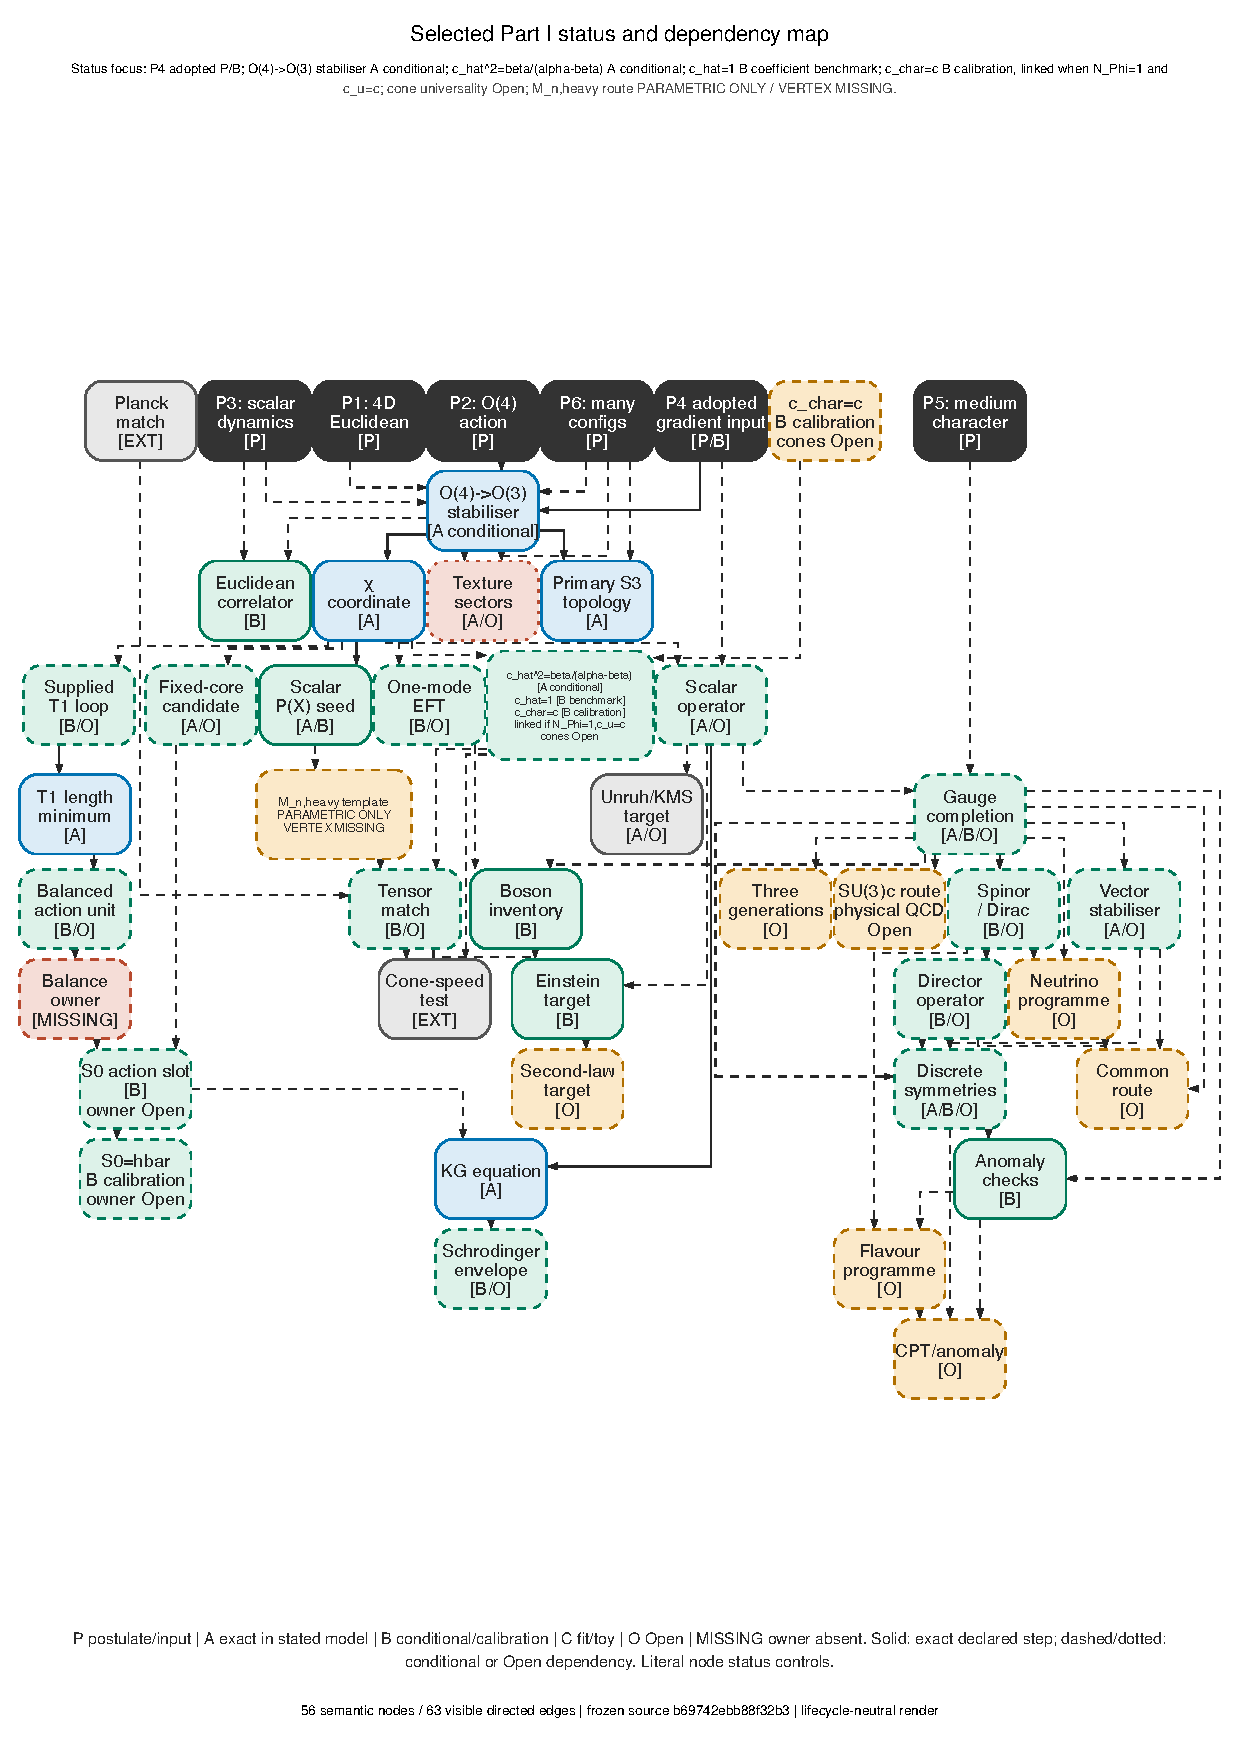
\includepdf[
  pages=1,
  fitpaper=true,
  pagecommand={\thispagestyle{empty}}
]{../figures/r185/logic_maps/partI_status_dependency.pdf}
\clearpage

%==============================================================
\part{Macroscopic Physics: Gravity, Cosmology, and Observational Tests}
\label{part:macro_pop}
%==============================================================

\section{Lorentzian kinematics in the homogeneous scalar/phase limit}

In the homogeneous ordered scalar/phase model, where the condensate amplitude
and direction are uniform, the characteristic metric reduces to the Minkowski
form after the proper-time map,
$ds^2=-c_{\rm char}^2d\tau^2+dx^2+dy^2+dz^2$.  Lorentz transformations and
the corresponding dispersion relation follow at Level~A inside this displayed
characteristic model.  ECT separately adopts $c_{\rm char}=c$ as a Level-B
scalar-clock calibration after fixing the conversion/lapse convention.  This
is not yet a derivation of physical special relativity for clocks, rods,
matter, photons or tensors: their kinetic operators, metric maps and
cross-sector cone equality remain Open.

\subsection{The scalar/phase characteristic-speed bound}

The ordered scalar/phase equation has a characteristic-speed bound that is not inserted as Einstein's second postulate. Its physical interpretation as the universal speed bound requires separate completion of every propagating sector.

The argument rests on the \emph{characteristic cone} of the ordered-branch scalar equation. Its principal symbol defines one cone with speed~$c_{\rm char}$. Under the stated hyperbolicity and regularity assumptions, the domain of dependence of that scalar problem is confined by this cone. The statement is Level~A inside the declared scalar/phase model; it does not assign the principal symbols of photons, gravitons, or general matter.

For linear plane waves, a massive mode has
$v_{\rm gr}<c_{\rm char}$ at finite wave number, with
$v_{\rm gr}\to c_{\rm char}$ at high wave number; a massless mode has
$v_{\rm gr}=c_{\rm char}$ for nonzero wave number.  This is a statement
about the centre of a narrow-band packet, not its causal front.  Because
the mass term is lower order, massive and massless modes have the same
front speed $c_{\rm char}$.  In flat $3+1$ dimensions the massive retarded
kernel has both a cone-boundary term and an interior tail, while the
massless retarded fundamental solution is supported on the cone.

The phase velocity of a massive mode formally exceeds $c_{\rm char}$,
but it transports neither information nor causal influence.  The scalar
causal bound is set by the characteristic/front speed, and its promotion
to a universal physical speed bound remains Open.

\subsection{Signal speed, not photon speed}

Within the scalar/phase model, the limiting velocity is the signal speed of its characteristic cone, not yet a photon-specific constant.

A physical photon may realise the scalar boundary speed after the gauge matching is completed.  The current action does not identify the gravitational-wave principal symbol, so GW170817 is an external tensor-completion gate rather than a structural ECT success.

Coordinate transformations preserving the homogeneous scalar/phase cone form the corresponding Lorentz group, so $c_{\rm char}$ is invariant within that characteristic geometry. Identifying this invariant cone with the physical light cone remains conditional on the unbroken gauge owner, its reduced Hessian and kinetic normalisation, and the matter/photon metric map.

The scalar calibration $c_{\rm char}=c$ is adopted only after the scalar
clock/lapse convention is fixed.  Identifying the photon cone with that
calibrated scalar cone additionally requires the photon action, reduced
Hessian, kinetic normalisation and observable metric; it does not follow from
the scalar principal symbol.


\section{Emergent gravity and the generalised Einstein equations}
\label{sec:pop_gravity}

In ECT geometry is not the primitive ontology.  The effective metric is a
low-energy bookkeeping object for propagation on the ordered medium.  ECT
adopts the Level-B/Open programme hypothesis $H_{N\to G}$: a future
macroscopic source tensor should arise by a declared metric-response and
coarse-graining map from a stationary full ordered-sector action, with
background subtraction, state and matching fixed.  The P3 Noether tensor is
not itself that universal matter-to-gravity vertex, and withdrawn off-shell
P3 density/pressure proxies are not physical cosmological sources.  The
controlled result relevant here is narrower than the older orientation-stress
narrative.

For the displayed scalar-only Jordan-frame ansatz, the consistently undivided metric equation can be written schematically as
\begin{equation}
  F\,G_{\mu\nu}
  = 8\pi G_*\,T_{\mu\nu}
    + \mathcal{T}^{(q)}_{\mu\nu},
  \label{eq:pop_gee}
\end{equation}
where $\mathcal{T}^{(q)}_{\mu\nu}$ collects the scalar derivative and
potential terms.  This entire equation uses $\hbar=c=1$:
$G_*\equiv(8\pi\bar M_{\rm Pl}^2)^{-1}$ and $T_{\mu\nu}$, $U$ are
natural-unit quantities.  Dividing the \emph{entire} equation defines the
natural-unit coefficients $G_{\rm div}=G_*/F$ and
$\Lambda_{\rm div}=U/(\bar M_{\rm Pl}^2F)$ as exact equation coefficients
inside the declared ansatz.  They are not by themselves Cavendish,
finite-body, or cosmological responses.  Those require scalar canonical
normalisation and range, body charges, the complete background and the
physical metric/clock map; matching $G_*$ to the observed $G_N$ is part of
that transfer.

Within the Level~B scalar ansatz, write $a(q)=f_{,q}/f$,
$\mathcal A=K+3f_{,q}^2/(2f)$, and
$\mathcal E=V_{,q}-2aV-(a/2)\rho_{\rm m}$.  On a fixed smooth root the
implicit-function theorem gives
$d\ln\bar f/d\rho_{\rm m}=a^2/(2\mathcal E_{,q})$ only when
$\mathcal E_{,q}\ne0$.  The sign is non-negative on the separate stable-root
branch $\mathcal E_{,q}>0$; $\mathcal A>0$ is an independent kinetic guard.
Then $m_{\rm loc}^2=\mathcal E_{,q}/\mathcal A$ is a conditional local
response, not a finite-body screening solution.  Freezing a homogeneous reference value
is an algebraic choice inside the ansatz, not a screening mechanism or a proof
that the reference is dynamically reached.

Three objects must remain separate. M is the microscopic operator $\mu_5\bar\Psi\gamma^A n_A\Psi$; S is this Level-B scalar ansatz; and G is the independently adopted Level-C galactic functional. M$\neq$S by operator/variable content, while the physical-coordinate, source, force, and normalisation map S$\to$G is Open.  The compact-source Yukawa theorem constrains only a separately supplied scalar operator and source; without its pole, coefficient and physical vertex it yields no galactic-distance verdict, while an extended driven profile remains a distinct case.

The displayed action contains no independent orientation field $n^A$ and therefore does not derive $T^{(n)}_{\mu\nu}$.  The form $\mathcal X^{\rm cand}_{\mu\nu}[n]$ is only an external proxy.  A physical orientation stress requires a separately specified covariant $S_n[g,n,\lambda_n]$, its constraints, and the full metric variation (\emph{Open}); the previously used projected-Riemann ``identity'' cannot replace those inputs.  Dividing Eq.~\eqref{eq:pop_gee} by $F$ changes only the normalization of terms already present and does not create an orientation source.

The scalar cosmological equations are exact inside their declared action. A named two-slope action gives conditional background, age, distance and high-redshift clock outputs; P1--P6 do not select a unique physical completion, and full Hubble/JWST inference remains Open. No orientation contribution has been calculated.  Practical galactic functional G is a separate Level-C fit.  The cluster script is only a local-map order/argmax audit and not a morphology closure; neither follows from Eq.~\eqref{eq:pop_gee}.  A canonical finite-body scalar charge, thin shell, Solar-System profile, and PPN projection remain Open.

A fixed-metric scalar boundary-value problem for the same named near-GR
two-slope state now supplies a narrower model-internal result.  At the
deliberately artificial scale $m_{\rm out}R=1$ and frozen
$(r,\eta)=(0.99,3333)$, its declared finite-window, asymptotic, and regular
$r\to1$ tail ratios are respectively
$0.006399711753$, $0.006393895852$, and $0.006372442154$.  These are three
different estimators or boundary limits, not measurements to be averaged.
Their publication-zone producer, independent verifier, and payload manifest
are respectively
\path{scripts/cosmology/compute_r114_twoslope_finitebody_estimators.py},
\path{scripts/verification/r114/verify_r114_twoslope_finitebody_estimators.py},
and \path{data/cosmology_r114/MANIFEST_SHA256_v1.json}.  This establishes
nonlinear far-tail suppression inside the supplied fixed-metric BVP; the
physical body charge, coupled metric, Cassini/WEP comparison, and full PPN
profile remain Open.

At fixed $\alpha,\beta$, about homogeneous $\bar n=w$, and to first order in a tangent director perturbation, the displayed map contains only mixed components $h_{iw}$ and has no linear TT/static-density seed: $h_{ij}^{\rm TT}=h_{ww}=0$.  This scoped Level-A negative result does not exclude quadratic, nonlinear, composite, nonlocal, additional-field or dynamical-$\alpha,\beta$ vertices.  An independent physical tensor completion --- constrained Hessian, matter source, positive residues, canonical normalisation, TT projector and nonlinear completion --- and the physical matter/photon metric map remain Open.


\section{Condensate evolution and cosmic history}
\label{sec:pop_evolution}

\begin{figure}[p]
\centering
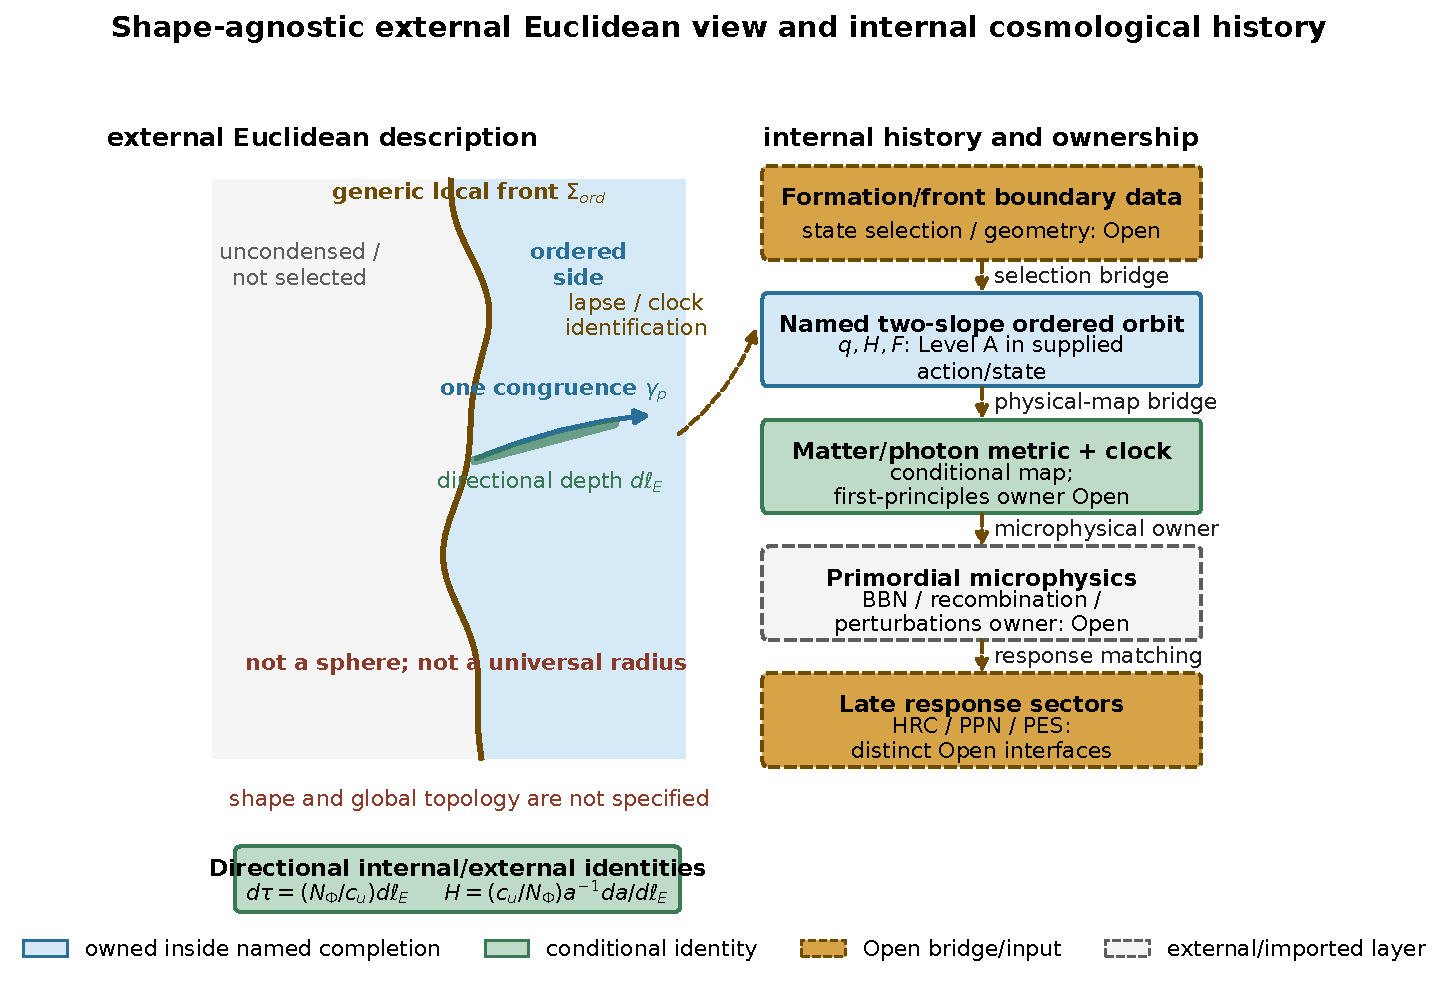
\includegraphics[width=\textwidth]{../figures/r149/r149_external_internal_history_map_typography.pdf}
\caption{\textbf{Shape-agnostic external/internal history map.}  The external
panel depicts a generic local formation front and one action-owned
congruence, not a spherical boundary or universal radius.  P4 supplies an
ordered direction and a candidate clock seed, but not the physical matter
congruence, lapse or clock map.  The displayed orbit is Level~A only inside
the named supplied action/state and coefficient assumptions; the
metric/clock map is conditional Level~B.  Formation, the physical
matter/photon metric, primordial and
Boltzmann owners, HRC/PPN matching and PES kernels remain Open.  Complementary
background panels are reference-ordered in the technical preprint appendix
\emph{Visual atlas: conditional background and cosmology}; the companion does
not duplicate that atlas.  Colour is redundant with border style and literal
status text.}
\label{fig:pop_timeline}
\end{figure}

In $\Lambda$CDM, the universe is modelled through a hot early phase,
primordial expansion, nucleosynthesis, recombination, structure formation and
late acceleration.  ECT has not yet derived a complete alternative history;
Fig.~\ref{fig:pop_timeline} records the owners still required.

The bare model uses a Euclidean arena without Lorentzian time; P4 then supplies an ordered-gradient analysis chart rather than a derived chronological transition.  The dimension-two gradient amplitude $u_0$ and the energy-dimension matching scale $\phi_0$ are distinct; no equation here sets $u_0=\phi_0$.  An ordering trajectory, physical branch selection, and any rapid-expansion phase require an explicit nonequilibrium completion and remain Open, so P4 is not a derived replacement for inflation.

Within a separately supplied post-order cosmological completion, familiar milestones are targets rather than derived outputs.  A regular two-slope scalar completion demonstrates that a radiation--matter--late-de-Sitter history is possible, while the physical ECT action, state, ordering history, full scalar--metric response history and late source remain Open.

A new conditional consistency condition follows within the same charge-selective architecture: if a physical ordered branch and charged completion are supplied, a neutral relaxing amplitude mode cannot directly populate the gauge/radiation bath unless charged degrees of freedom are available. The candidate sequence is therefore
\[
\text{gradient ordering}
\to
\text{metric/\(\Phi\)-sector matching}
\to
\text{charged-spectrum population}
\to
\text{entropy production}.
\]
This is only a post-onset routing constraint; it does not specify an efficiency, timescale, or detailed thermalisation mechanism, and it makes no statement at the pre-emergent Euclidean level.

A notable conceptual distinction is the \textbf{age of the Lorentzian
branch}.  ECT defines it as the duration from a physical ordering event,
\[
t_{0,\rm ECT}=\int_{a_{\rm ord}}^1{da\over aH_{\rm ECT}(a)}.
\]
The universal postulates need not select the integration constants or the
dimensional unit of our realised condensate.  A completed action must instead
derive the matter-clock congruence and external depth/lapse map and then test
one declared state.  The supplied two-slope completion gives the conditional
value $\tau_{2s}\equiv H_{2s}(0)\Delta t=0.96368678$ and direct high-redshift clock budgets; these are
ECT-candidate state outputs, not one universal law-level age.  Every distance
and structure calculation must use that same
globally regular background and disclose the extra metric/perturbation inputs.


\begin{figure}[p]
\centering
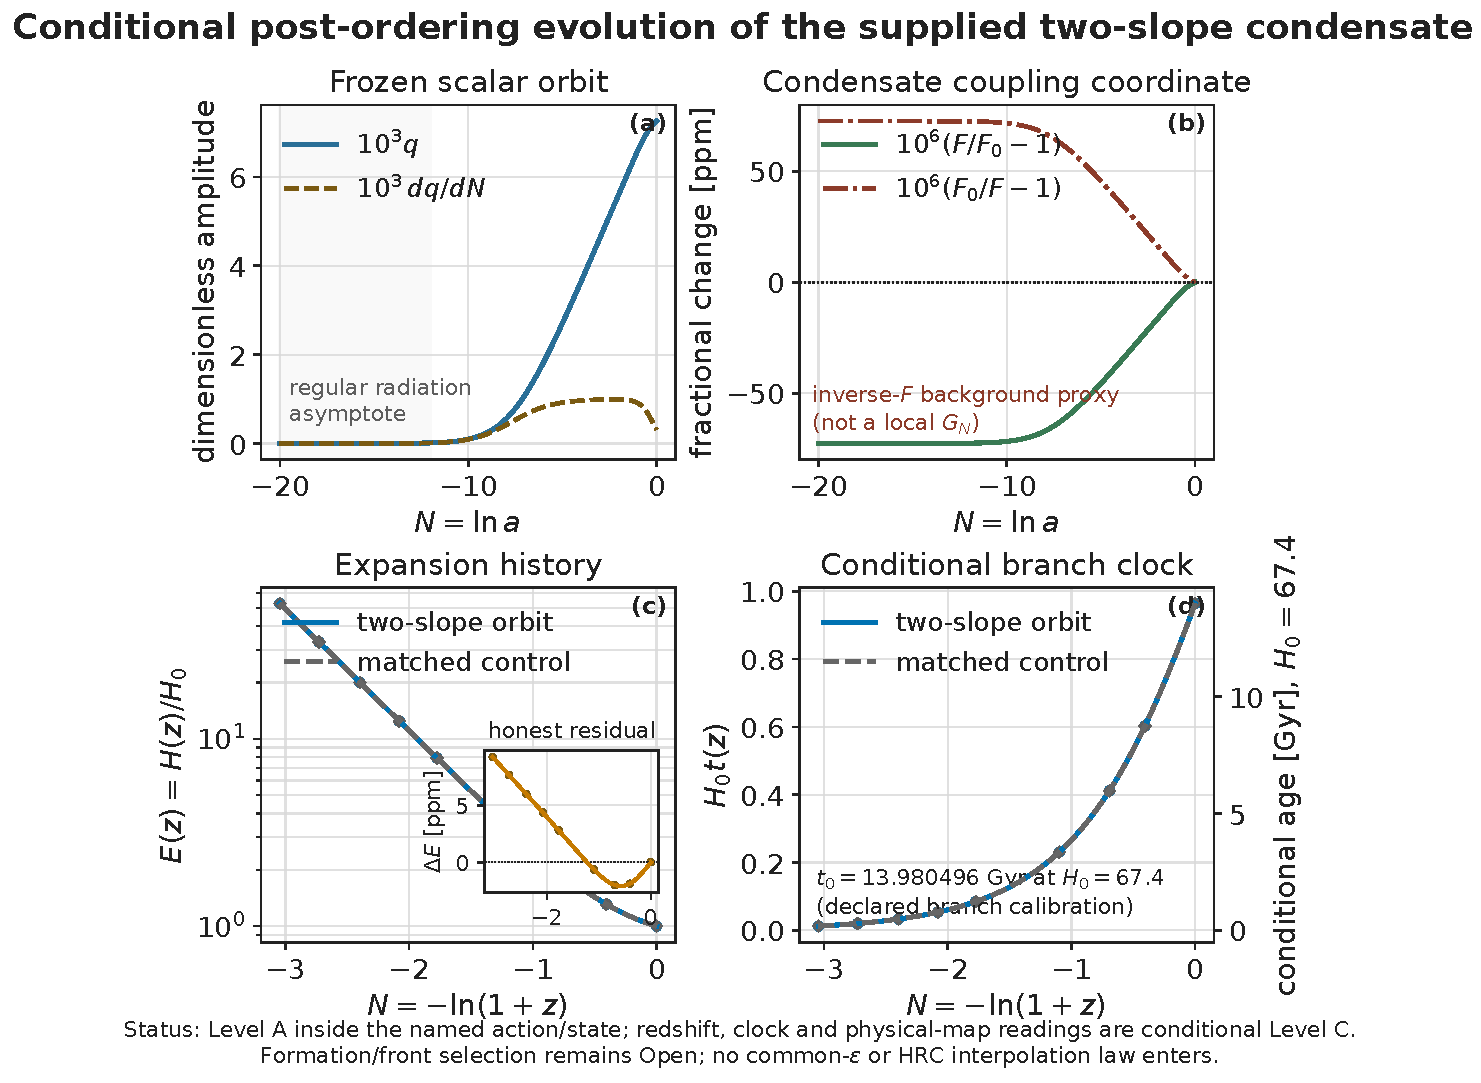
\includegraphics[width=\textwidth]{../figures/r154/curve_semantics/nonrotation/conditional_post_ordering_dense_r154.pdf}
\caption{\textbf{Conditional post-ordering orbit of the supplied two-slope
completion.}  The symbol $\sigma$ in this figure denotes the dimensionless
coordinate of the named two-slope completion; it is not the microscopic
radial fluctuation $\sigma=u-u_0$ used elsewhere.  The inverse-$F_s$ curve is
a background proxy, not a locally measured $G_N$.  Dynamical curves are
Level~A only inside the supplied action/state and coefficient assumptions;
redshift, Gyr and physical-map readings are Level~C conditional on the
declared dimensional calibration.
The integration starts on an already ordered regular radiation branch and
does not derive the Open formation front.  Panels~(c), its inset and~(d)
show nine evaluated redshift nodes as unconnected markers; no intermediate
interpolation is implied.  \textit{Display semantics: \detokenize{Panels (a,b) are dense frozen solver histories without decorative markers; panels (c,d) use solver-owned dense background traces with the nine published diagnostic nodes shown separately.}}}
\label{fig:pop_conditional_post_ordering_orbit}
\end{figure}

\begin{figure}[p]
\centering
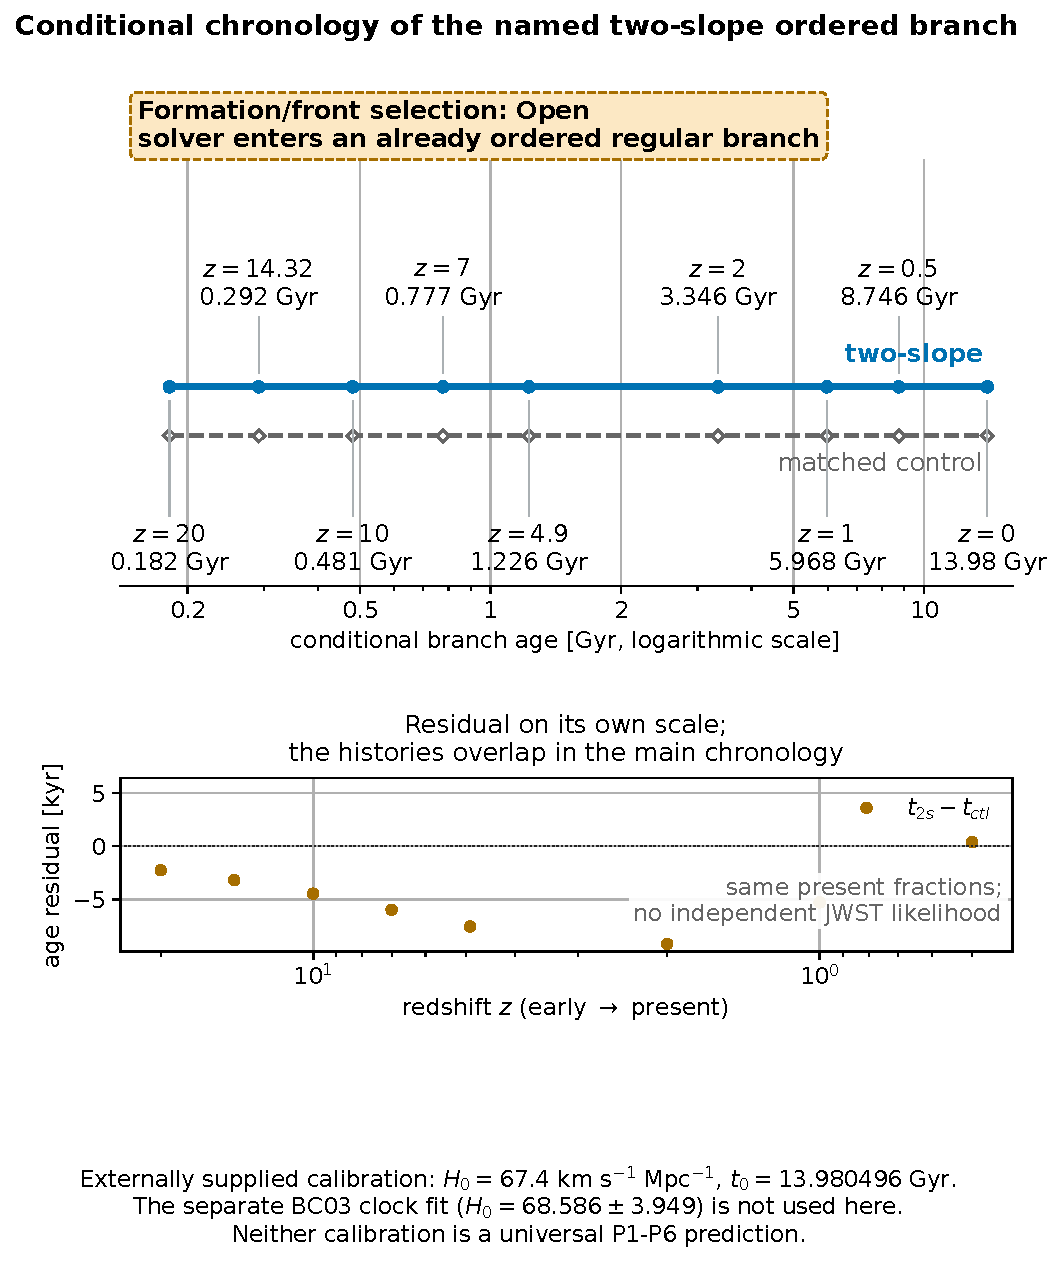
\includegraphics[width=\textwidth]{../figures/r153/line_semantics/conditional_chronology_nodes_r153.pdf}
\caption{\textbf{Conditional chronology of the named two-slope ordered
branch.}  At the single externally supplied calibration $H_0=67.4\,
\mathrm{km\,s^{-1}\,Mpc^{-1}}$ the displayed state has
$t(z=10)=0.4814276482\,$Gyr and $t_0=13.9804960874\,$Gyr.  These numbers
share one external dimensional calibration and are neither universal P1--P6
ages, a Hubble-tension solution nor a JWST abundance calculation.  The
formation front, BBN/recombination microphysics and physical metric/clock map
remain Open.  The residual panel shows nine evaluated event redshifts as
unconnected markers; no intermediate residual interpolation is implied.}
\label{fig:pop_conditional_chronology}
\end{figure}
Profiling its single dimensional scale against the official 15-point BC03
cosmic-chronometer subset with the suggested covariance gives the conditional
calibration $H_0=68.59\pm3.95$ km\,s$^{-1}$\,Mpc$^{-1}$ and
$t_0=13.74\pm0.79$~Gyr (linearised $H_0$-only uncertainty).  This Level-C result calibrates one realised orbit;
it is neither a universal postulate-level age nor a resolution of the Hubble
tension, and the matched flat control is observationally indistinguishable.

At late times, qualitative expanding or recollapsing scenarios remain
possible, but their timescales require the missing cosmological completion.

\section{The four classical cosmological problems}
\label{sec:pop_cosmo_problems}

The standard hot-Big-Bang extrapolation motivates four well-known early-universe
puzzles.  Inflation is the conventional dynamical solution class.  Its model
space has separate questions about initial conditions, measures in eternal
inflation, and ultraviolet sensitivity.  In sufficiently long or high-scale
inflationary histories, backward extrapolation can place observable modes
below the Planck length; this conditional trans-Planckian concern is not a
property of every inflationary history.

ECT organises structural or conditional non-inflationary candidate routes to
the four puzzles; it does not yet supply a complete dynamical replacement for
inflation or a physical primordial-spectrum prediction.

\subsection{The horizon problem}

The cosmic microwave background (CMB) --- relic radiation from about
380\,000 years after the Big Bang --- is uniform to one part in $10^5$ across
the entire sky.  In a decelerating hot-Big-Bang extrapolation with no earlier
causal mechanism, sufficiently separated last-scattering regions have
non-overlapping past light cones.  Inflation is the standard solution class;
other proposed early-universe mechanisms exist, so the observation does not
logically select inflation alone.

The P1 Euclidean configuration class contains no supplied Lorentzian
light-cone horizon; that is an exact statement about the declared
configuration class.  Interpreting it as a physically earlier epoch and
demonstrating that the observed CMB uniformity is inherited by a later
physical metric require ordering dynamics, a clock, a state and thermal
transfer, and remain Level~B/Open.

A useful condensed-matter analogy is a ferromagnet. Below the critical temperature, a sufficiently coherent domain orders as one region, and distant points inside that domain share the same orientation not because they exchanged late-time signals, but because they belong to one ordered phase.  ECT motivates the corresponding candidate: a sufficiently coherent pre-Lorentzian ordering domain could seed correlated initial data. Whether the observed CMB uniformity is inherited requires a supplied state, nonequilibrium ordering history and transfer calculation and remains Level~B/Open.

\subsection{The flatness problem}

Observations constrain the present spatial-curvature parameter tightly
(for example, the cited Planck+BAO analysis gives
$\Omega_K=0.001\pm0.002$ at 68\% confidence).  A quoted
early-time ``fine-tuning'' factor is meaningful only after an initial slice,
background history and measure on initial data have been specified; no
stand-alone $10^{-60}$ inference is used here.

P1 chooses a flat Euclidean substrate ($\delta_{AB}$).  This gives a candidate flatness route, but does not by itself prove the curvature of the emergent cosmological branch; the geometric/dynamical transfer is Level~B/Open.

\subsection{The relic and monopole problem}

Grand Unified Theories can predict massive topological defects (magnetic monopoles). None has been observed.  For the supplied P4 orientation target $S^3$, $\pi_2(S^3)=0$, so maps into that target carry no $\pi_2$ topological charge (A-math conditional).  Identifying $S^3$ with the complete physical cosmological vacuum/configuration space and deriving a formation history are Open; therefore no physical ECT monopole anti-prediction follows yet.  Later gauge-completion sectors have their own topology and abundance owners.

\subsection{The primordial perturbation problem}

The CMB contains tiny fluctuations ($\sim 10^{-5}$) with a nearly
scale-invariant spectrum ($n_s = 0.9649 \pm 0.0042$, Planck 2018).  At linear
order on a smooth patch of the strict scalar-only pullback, integrability
parametrises the soft ordering variation by one scalar coordinate~$\chi$
(Level-A conditional kinematics).  Whether it is a propagating physical mode,
and whether it is the only scalar of the completed theory, requires a supplied
reduced action, constraint/boundary quotient and physical projector
(Level~B/Open).  An ordinary $O(4)$-critical correlator does \emph{not} by
itself give the observed spectrum: it projects to a blue tilt.  For the
separately supplied translation-invariant pure-quartic strict-pullback kernel
with constant $Z_u,\mathcal C_n>0$, vanishing lower-order deformations,
$k>0$ and a controlled zero mode, the formal local equal-slice seed is exactly
$P_\chi\propto k^{-3}$ and hence $n_\chi=1$ (Level-A conditional
mathematics).  With lower-order terms, positivity alone is insufficient: the
exact $(\delta_a,\delta_m,\rho)$ amplitude and bandwise tilt bounds must hold
throughout a finite quartic-dominance band above the infrared crossovers and
below the EFT ultraviolet validity limit.  The existence of this band, a
physical reflection-positive covariance and state, the coefficient owner and
running, the $\chi\to\zeta$ transfer, and the observed $n_s,A_s,r$ remain
Open.

A separate low-multipole branch may be retained only as an Open completion
ansatz: a supplied low-$k$ window, scale and signed amplitude would have to be
propagated through one gauge-invariant perturbation, recombination/Boltzmann
and likelihood chain.  An ordering/coherence scale does not by itself select
suppression, and P1--P7 predicts neither its sign nor a CMB quadrupole value.

\subsection{Summary}

The four classical puzzles are reformulated without introducing an inflaton
field.  The pre-Lorentzian Euclidean configuration class gives a structural route to
horizon-scale homogeneity; the flat Euclidean substrate gives the baseline
flat branch; and the supplied $S^3$ orientation target has $\pi_2(S^3)=0$.
The physical vacuum-manifold, transition and relic conclusions remain Open. In the
perturbation route, a supplied pure-quartic ordering-sector kernel gives an
exactly flat formal local seed, while the physical finite band, state,
transfer and observed primordial spectrum remain Open.  The first-principles
probability of selecting the required coherent branch and the full
quantitative derivation of $(n_s,r,A_s)$ remain open.


\section{The dark sector in ECT}
\label{sec:pop_dark}

The terms ``dark matter'' and ``dark energy'' organise observations that
visible matter plus standard gravity does not account for by itself: rotation
curves, gravitational lensing, large-scale structure and accelerated
expansion.  No dark-matter particle has been identified.  A rigid $\Lambda$
fits the background data well but is not uniquely established as a
microscopic vacuum source.  The present ECT applications are separate closure
layers.  The adopted Level-C galactic functional contains no particle-halo
term, but its ECT matching and fundamental particle content remain Open; the
late-time background closure has its own declared status.

\subsection{Galactic no-halo fit and Open particle content}

In $\Lambda$CDM, the flat rotation curves of galaxies, gravitational lensing in clusters, and the large-scale structure of the universe are attributed to an invisible component --- dark matter --- constituting roughly one quarter of the energy budget.  Broad direct, indirect and collider searches have not established a dark-matter particle.  Direct-detection experiments such as LZ strongly constrain standard WIMP parameter space, but a null search does not establish the absence of every particle or hidden-sector completion~\cite{LZ2023,ParticleDataGroup2022}.

The galactic mass-discrepancy results come from the HRC-only algebraic implementation of functional G (Level~C), not from the corrected scalar trace equation or a derived orientation stress.  Rotation-curve and BTFR/RAR statements retain their fit/conditional status.  The separate cluster script is only an exact order/argmax-preservation audit of hand-set maps and supplies no morphology evidence.  The physical S$\to$G source/force map and any $T^{(n)}_{\mu\nu}$ remain Open.


\subsection{Late-time acceleration: conditional scalar example, physical owner open}

Observed late-time accelerated expansion is an empirical target.  In
$\Lambda$CDM it is represented by a cosmological constant.  The current ECT
action does not yet identify the physical late-time source, its state, or its
equation-of-state history.

Inside the supplied positive-kinetic scalar action the dimensionally
normalised bare pieces use
$K_\phi^{\rm phys}=\bar M_{\rm Pl}^2\omega\dot\phi^2/2$ and obey
\[
 \rho_\phi^{\rm bare}=K_\phi^{\rm phys}+U,\qquad
 p_\phi^{\rm bare}=K_\phi^{\rm phys}-U,\qquad
 w_\phi^{\rm bare}\ge-1
\]
when $\omega>0$ and the bare denominator is positive.  This is an exact
bookkeeping identity, not an acceleration theorem: $\dot F$ and $\ddot F$
enter the full scalar--tensor expansion history.  The local corrected result
shows that the observable $w_{\rm eff}$ is not bounded below by $-1$ and can
lie below $-1$; it does not construct or select a global crossing history.
A physical ECT result requires one stable action-owned background and the
complete distance, growth, photon and lensing likelihood.

The exact fixed determinant concerns only the fixed-coefficient
orientation submanifold and does not prove vacuum decoupling.  An explicitly
supplied trace-free completion is classically shift covariant through
$V+C_I$, while the distinct two-slope completion provides a regular
late-acceleration proof of class but is not shift invariant.  Their descent
from the $\Phi$ medium, the physical metric and the source/state of the
observed acceleration remain Open.

\subsection{ECT reinterpretation of the dark sector}

The adopted Level-C galactic functional fits selected mass-discrepancy benchmarks without a particle-halo term. This is a property of that fit model, not an ECT derivation or an inference that particle dark matter is absent. Its scalar matching, cosmological fraction budget, and fundamental particle content remain Open. A particle species independently shown to explain the galactic discrepancy would reject the minimal no-halo fit interpretation, not ECT as a whole; null direct-detection searches do not confirm the closure. The late-time background is a separate closure and must not be merged with this ontology statement.



\section{The Hubble tension}
\label{sec:pop_hubble}

The measured expansion history is a real target for ECT, but the current
theory does not yet predict a numerical $H_0$ shift.  A genuine calculation
must derive one ordered-branch background, the physical photon metric,
recombination and the sound horizon, and must analyse early- and late-time
data in one likelihood.  The scalar-only background equations are exact
inside their declared model, yet their closure functions, orientation stress,
state and initial data are not fixed by P1--P6.  They therefore permit many
different $H(z)$ histories.

The age of the Universe is correspondingly not a number that can be imported
from a reference cosmology.  ECT defines it along the physical matter
congruence from the ordered-side branch-formation front,
\[
 t_{0,\rm ECT}=\int_{a_{\rm ord}}^1{da\over aH_{\rm ECT}(a)}.
\]
The outside description is the corresponding clock-lapse integral over
Euclidean arc length.  P1--P6 need not select the integration constants or
unit scale of our realised state; the completion must derive the congruence,
physical metric and depth/lapse map.  The supplied-completion estimates below
are therefore conditional ECT-candidate ages, not one universal law-level
number.

A useful existence result survives this ceiling.  A fully specified
two-exponential scalar--tensor action with positive kinetic determinant has
an exact frozen-radiation branch, an exact dust tracker, one stable late-time
vacuum, and a two-solver trajectory connecting the three regimes without an
attached high-redshift background.  This is a proof that a regular scalar
completion exists in the nearby model class.  It is not yet the ECT
background: the microscopic theory has not derived that action, physical
metric and clock map.  The dimensionless clock integral is a conditional age
of that ECT-candidate state rather than a universal P1--P6-selected value.
For a second near-GR member of that same supplied family the model-owned
dimensionless interval is $\tau_{2s}\equiv H_{2s}(0)\Delta t=0.9636867786$; a disclosed conditional dimensional scale calibration
to $H_0=67.40$ or $73.04\,\mathrm{km\,s^{-1}\,Mpc^{-1}}$ gives respectively
$13.9805$ or $12.9010$~Gyr.  These are conditional ages of the named
completion, not a unique ECT prediction.

The same orbit directly gives $E(z)=H(z)/H(0)$, distances and high-redshift
clock budgets.  For the $67.40$ conditional dimensional scale calibration its ages at
$z=(4.9,7,10,14.32,20)$ are
$(1.2265,0.7769,0.4814,0.2924,0.1818)$~Gyr.  Under explicitly imported
standard photon/recombination inputs it changes the sound horizon by only
$-0.00316\%$ relative to the matched control.  A restricted quasistatic
growth diagnostic changes the normalised growth by less than
$0.002\%$ through $z=20$.  In a still more restricted same-metric,
zero-slip, sub-horizon closure, the instantaneous Weyl-amplitude carrier
changes by only $0.00267$--$0.00292\%$ and its conformal-derivative carrier
by $0.00308$--$0.00813\%$ over $0\le z\le2$.  These are not projected
lensing or horizon-scale ISW predictions.  These conditional numbers show that this
near-GR member neither materially shifts Hubble inference nor resolves early
maturity.

At the nine prespecified computed nodes, every change in the
high-redshift clock is negative (down to $-10.491167\%$ at $z=10$), while
larger sampled acoustic leverage accompanies larger homogeneous
$G_{{\rm div},s}$/Planck-factor drift.  A $-5.55\%$ sound-horizon node has
$|\gamma_{\rm PPN}-1|=0.0174$ in the distinct unscreened local-response proxy,
whereas the only sampled node satisfying the displayed zero-centred
absolute-deviation proxy changes $r_s$ by $-0.00323\%$; this is not a full
Cassini likelihood.  The divided coefficient and the PPN proxy must not be
identified.  The finite scan is a useful action-owned benchmark.  It neither
proves a continuous-family no-go nor supplies a JWST-abundance or
Hubble-tension solution.

Separately, an owner-specific five-row early-response envelope tests a
constant coordinate $\zeta_{\rm ER}$ without identifying it with the named
two-slope orbit or with a universal ECT parameter.  The radiation term is
deliberately left unmodified as an imported guard, not as derived radiative
protection.  At $z=10$ the five prescribed rows give
\begin{center}
\small
\begin{tabular}{@{}r r r r r@{}}
\toprule
$\zeta_{\rm ER}$ & $D/D_0$ & $(1+z_{\rm eq})/(1+z_{\rm eq,0})$ &
$\delta_c$ & $R_{\rm PS}^{\rm top\mbox{-}hat}$\\
\midrule
$1.5612556\times10^{-6}$ & 1.000005 & 1.000025 & 1.726760 & 1.000131\\
0.00750044 & 1.024950 & 1.131953 & 1.728110 & 1.830827\\
0.02958834 & 1.097679 & 1.668466 & 1.732341 & 8.515859\\
0.03300000 & 1.108822 & 1.777309 & 1.733025 & 10.502280\\
0.03755500 & 1.123667 & 1.936589 & 1.733951 & 13.755949\\
\bottomrule
\end{tabular}
\end{center}
The background/equality algebra and the linear-growth integration are exact
or reproducible only inside this supplied envelope.  The top-hat barrier and
Press--Schechter rare-tail ratios are Level-C sensitivity estimates.  The
five rows are not posterior samples, a JWST abundance prediction, or a
likelihood; in particular, the boosted rows also shift the declared equality
coordinate by about $13$--$94\%$.

\begin{figure}[H]
\centering
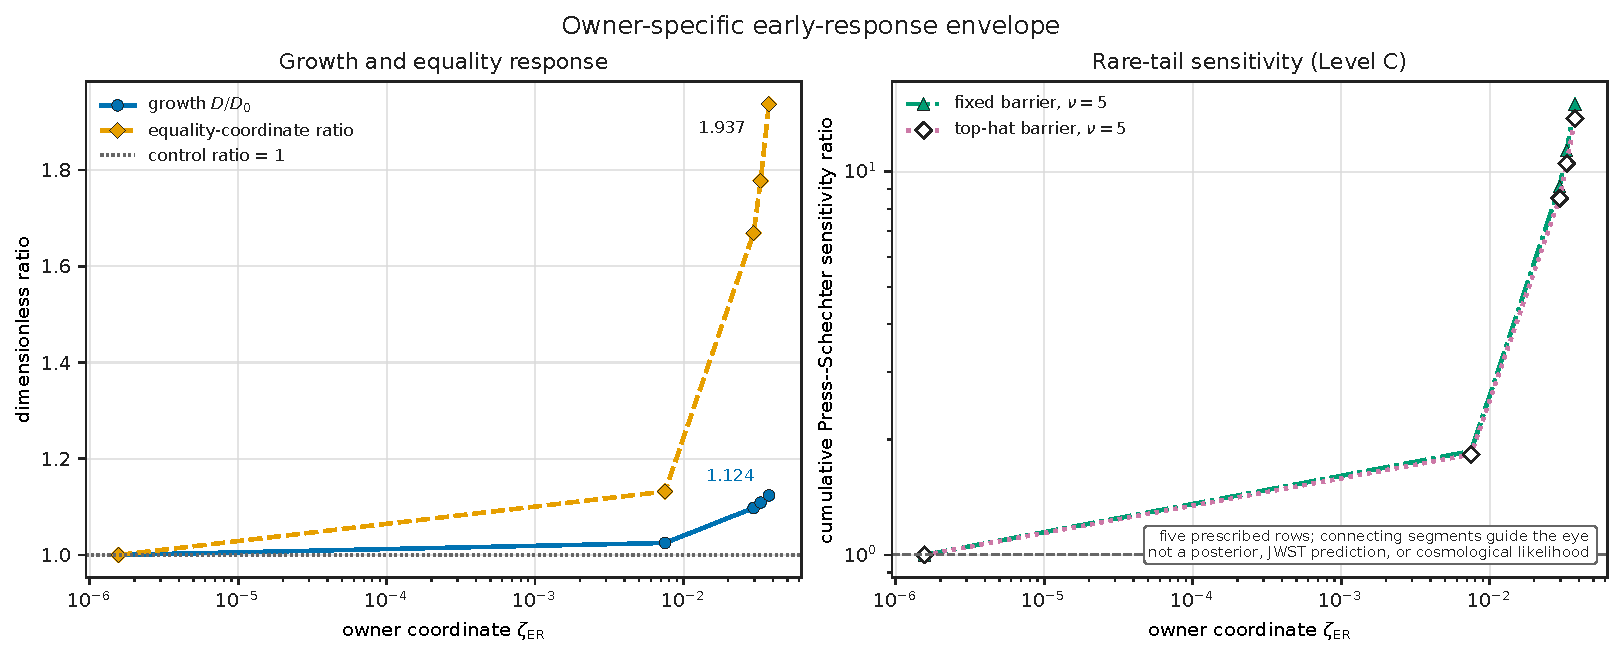
\includegraphics[width=0.98\textwidth,trim=0 0 389.4bp 26bp,clip]{r114/r114_early_response_growth_collapse_envelope.pdf}
\caption{Owner-specific early-response sensitivity envelope: growth and
equality response for the five prescribed stress-test rows.  This is an
enlarged crop of the frozen left panel; no data or styling have been
recomputed.  The response is conditional on the supplied envelope.  Lines
guide the eye between the five rows; they do not define a posterior, JWST
prediction, or likelihood.  Colour is redundant with marker and line style
for grayscale-safe reading.}
\label{fig:pop_r114_early_response_envelope}
\end{figure}

\begin{figure}[p]
\centering
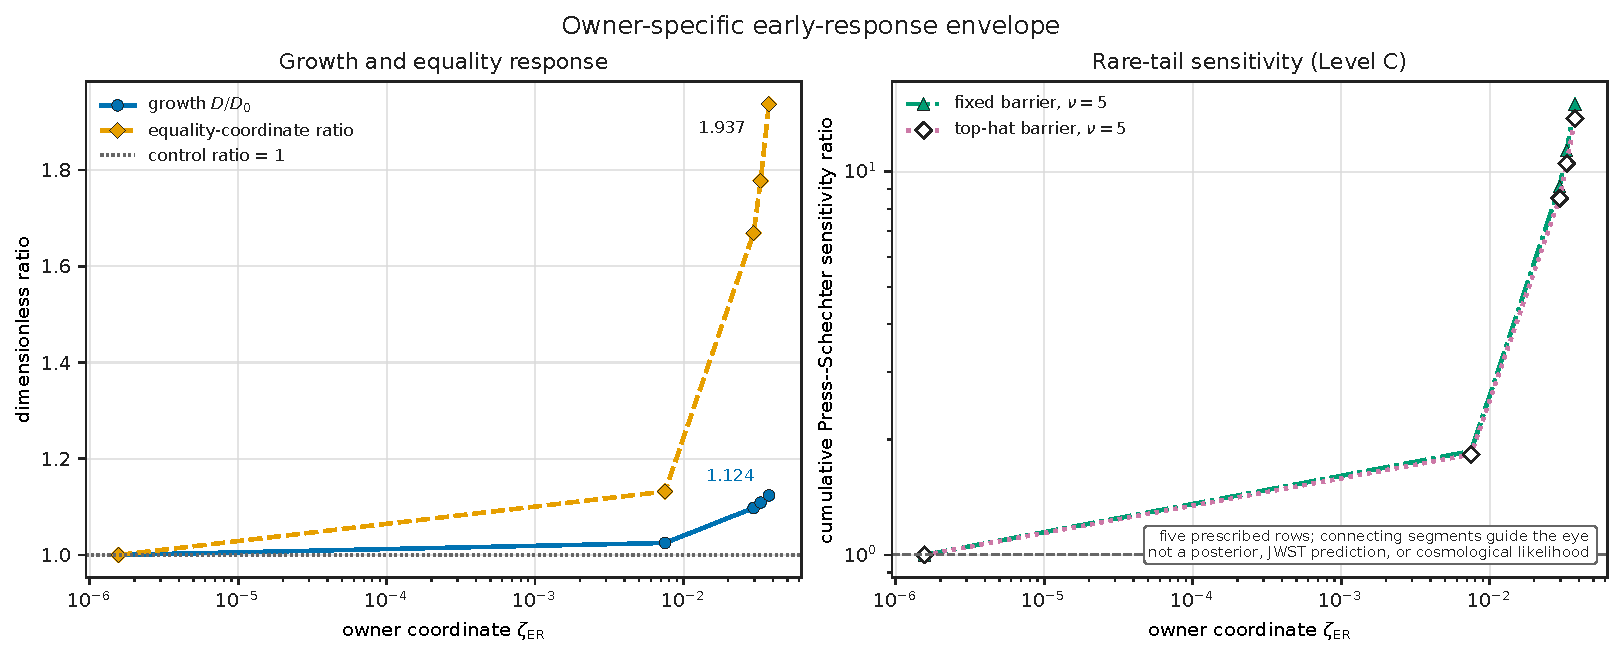
\includegraphics[width=0.98\textwidth,trim=389.4bp 0 0 26bp,clip]{r114/r114_early_response_growth_collapse_envelope.pdf}
\caption*{\textbf{Readable detail of Fig.~\ref{fig:pop_r114_early_response_envelope}: collapse and rare-tail response.}  This is an enlarged crop of the frozen right panel; no data or styling have been recomputed.}
\end{figure}
\FloatBarrier

HRC addresses a separate quasistatic galactic response after an additional
gravity bridge.  It does not provide the homogeneous stress tensor or the
cosmological perturbation equations, and a possible relation
$a_M\propto cH$ remains a matching hypothesis until one action yields both.

\section{The JWST early-galaxy problem}
\label{sec:pop_jwst}

Early massive objects cannot be predicted by changing one background
response factor.  ECT must derive the time and volume elements, primordial
spectrum, transfer and scale-dependent growth, non-linear halo abundance,
baryonic mass-to-light relation and survey selection.  None of these may be
replaced by an independently tuned common parameter.  The present result is
therefore an explicit programme and falsifier list, not a claimed JWST
resolution: an accepted completion must reproduce the observed abundance and
morphology with the same action and state that pass Hubble, lensing, growth
and local-gravity gates.

\section{HRC galactic response and rotation curves}
\label{sec:pop_galaxies}

The current galactic programme uses the HRC response hierarchy.  Its
logical chain is deliberately layered:
\begin{equation}
 \begin{aligned}
 \underbrace{\text{S11a/S11b: local deformation / finite paths}}_{\text{kinematical / candidate}}
&\ \not\Longrightarrow
 \underbrace{\text{ERP-$\Phi$}}_{\text{separately supplied constitutive specialisation}},
 \\[-1pt]
 \underbrace{\text{ERP-$\Phi$}}_{\text{ideal constitutive specialisation}}
&\ \Longrightarrow
 \underbrace{\text{HRC}}_{\text{dimensionless response}}\\[-1pt]
 &\ \xrightarrow{\text{separate matching}}
 \underbrace{\text{weak-field gravity}}_{\text{conditional}} .
 \end{aligned}
 \label{eq:pop_hrc_hierarchy}
\end{equation}
S11a states only the guarded local tangent-space property.  S11b separately
allows finite admissible branch paths but supplies neither a dissipative law
nor dynamical accessibility.  Neither contains gravity, force, metric or
acceleration.  ERP-$\Phi$ is narrower: in an ideal quasistatic,
zero-temperature and non-hysteretic response sector, equivalent normalised
channels receive one common scalar shift and a channel is recruited when its
stability eigenvalue crosses zero.  Positive inverse-DtN compliance supplies
its static weight, and a positive semifinite trace adds recruited channels.
These clauses are a Level-B candidate constitutive extension, not a result of
the frozen P1--P6 action.  In particular, the P4 background is not stationary
under the frozen P3 action, so a physical constrained response Hessian still
requires a stationary ordered-phase action.

For the homogeneous three-dimensional spectral model the primitive and
response are
\begin{align}
 W_0(s)&=\sqrt{s(1+s)}-\operatorname{arsinh}\sqrt{s},\\
 \widehat\mu_0(s)&=\frac{dW_0}{ds}=\sqrt{\frac{s}{1+s}} .
 \label{eq:pop_hrc0}
\end{align}
This HRC-0 result is exact inside the stated augmented
inverse-DtN/recruitment model.  Algebraically, with $x=\sqrt{s}$, it is
exactly the conventional MOND-standard interpolation
$x/\sqrt{1+x^2}$; HRC-0 therefore introduces no new galaxy-level
interpolation shape.  The proposed response owner and the Open scale/gravity
bridges, not this algebraic function, are the distinctive ECT programme.
A supplied equal-three-channel ($n_{\rm ch}=3$), rank-one response gives
\begin{equation}
 \widehat\mu_3(s)=\widehat\mu_0(s)
 \left[1-\frac43\frac{s}{(1+s)^2}\right] .
 \label{eq:pop_hrc3}
\end{equation}
Here $n_{\rm ch}=3$ and $r_{\rm ch}=1$ are respectively the channel count and
selected-projector rank, so the matrix coefficient is
$4r_{\rm ch}/n_{\rm ch}=4/3$.  These integers belong to the supplied matrix
model; they are not fitted galaxy parameters.
HRC-3 is Level~A inside that supplied matrix model and a Level~B
proof-of-class, but its three-channel owner is Open in P1--P6.  It was
constructed after the crossover residuals were inspected and therefore is
\emph{not} an independent observational prediction.

Finite coupling need not shift the threshold in one precisely defined
factorised class.  Let $\widehat\Lambda$ be the dimensionless constrained
stability operator, let $C>0$ be a static compliance satisfying
$[C,\widehat\Lambda]=0$, and let $\tau$ be the positive semifinite trace.
Define
\begin{equation}
 \widetilde\Omega_s[\mathcal Q]=
 \tau\!\left[C^{1/2}(\widehat\Lambda-sI)C^{1/2}\mathcal Q\right],
 \qquad 0\le\mathcal Q\le I,\qquad
 P_s=\mathbf 1_{(-\infty,s)}(\widehat\Lambda),
 \label{eq:pop_hrc_finite_probe}
\end{equation}
Then the crossing set is unchanged,
$\mathcal Q_{*,s}=\arg\min_{0\le\mathcal Q\le I}
\widetilde\Omega_s[\mathcal Q]=P_s$, and
$-d\widetilde\Omega_*/ds=\tau(CP_s)$.  This is Level~A inside the supplied
factorised commuting model and a Level-B closure route.  It is not unique:
any positive $h(\widehat\Lambda)$ has the same threshold property, while a
generic non-commuting readout/source term shifts crossings.  The physical
choice $C=(1+\widehat\Lambda)^{-1/2}$ and its action owner remain Open in
P1--P6.

A second mandatory guard concerns the infrared limit.  Compactness of an
interface alone does not imply a discrete or gapped spectrum.  If the
constrained stability operator is self-adjoint with compact resolvent, all
physical zero modes have been removed, and its first retained eigenvalue is
strictly positive, then recruitment on the finite interface is a staircase
with an infrared gap.  Under those additional hypotheses, smooth deep-HRC
behaviour requires the continuum/thermodynamic limit before $s\to0$, or a
noncompact or gapless internal fibre.  No spherical cosmic boundary is
assumed.  The HRC formulas below describe that stated continuum response
model, not a generic finite interface.

Only after this internal response has been defined is a gravitational layer
introduced.  With
\begin{equation}
 Y_g=\frac{|\boldsymbol\nabla\Phi_{\rm gal}|^2}{a_M^2},\qquad
 s=f(Y_g),\qquad
 \mu_g=A_g\widehat\mu_\Phi(f)f',
 \label{eq:pop_hrc_bridge}
\end{equation}
the computations below declare the identity bridge $f(Y_g)=Y_g$, $A_g=1$.
That bridge, the baryonic matter vertex, the photon/metric map and the origin
of $a_M$ are Open.  The static conditional functional gives
\begin{equation}
 \boldsymbol\nabla\!\cdot
 [\mu_{g,k}(Y_g)\boldsymbol\nabla\Phi_{\rm gal}]
 =4\pi G_N\rho_b,
 \qquad k\in\{0,3\}.
 \label{eq:pop_interp}
\end{equation}
The present matching value
$a_{M0}=cH_0/(2\pi)\simeq1.08\times10^{-10}$\,m\,s$^{-2}$ for
$H_0=70$\,km\,s$^{-1}$\,Mpc$^{-1}$ is an explicit input, not a medium
postulate or derived coefficient.  The stronger law $a_M(z)\propto H(z)$ is
a separate hypothesis and is not assumed here.

\begin{figure}[p]
\centering
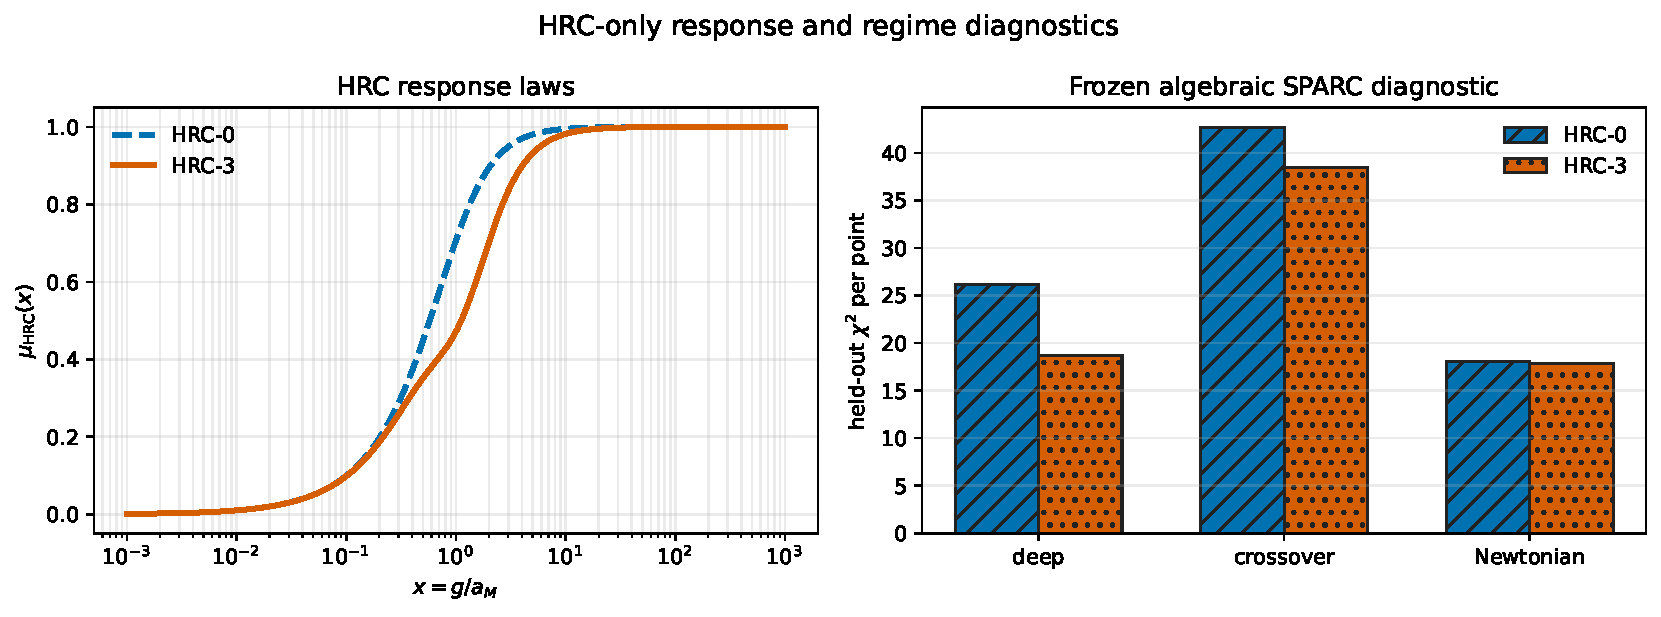
\includegraphics[width=0.98\textwidth,trim=0 0 398.653bp 26bp,clip]{hrc/R97_HRC_RESPONSE_AND_REGIMES.pdf}
\caption{HRC-only response functions.  HRC-0 is exact inside the stated
augmented response model; HRC-3 is conditional on the supplied three-channel
owner.  This is the enlarged frozen left panel of the response-and-regime
diagnostic; no curve or fitted quantity has changed.  Colour is redundant
with line style and direct labels.}
\label{fig:pop_hrc_response}
\end{figure}
\begin{figure}[p]
\centering
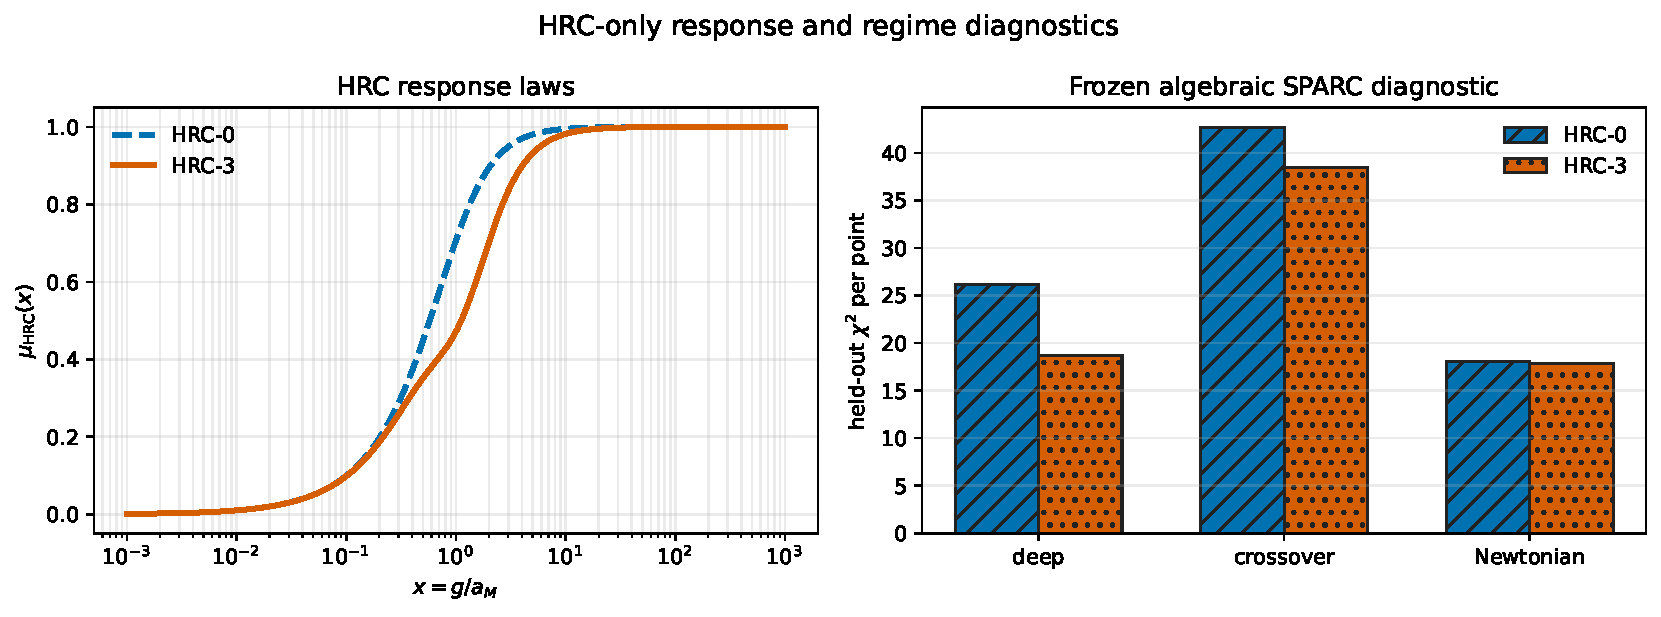
\includegraphics[width=0.98\textwidth,trim=398.653bp 0 0 26bp,clip]{hrc/R97_HRC_RESPONSE_AND_REGIMES.pdf}
\caption*{\textbf{Continuation of Fig.~\ref{fig:pop_hrc_response}: regime and
held-out residual diagnostics.}  The absolute held-out residual scale is
displayed rather than hidden.  This is the enlarged frozen right panel; no
curve or fitted quantity has changed.}
\end{figure}
\FloatBarrier

\begin{figure}[p]
\centering
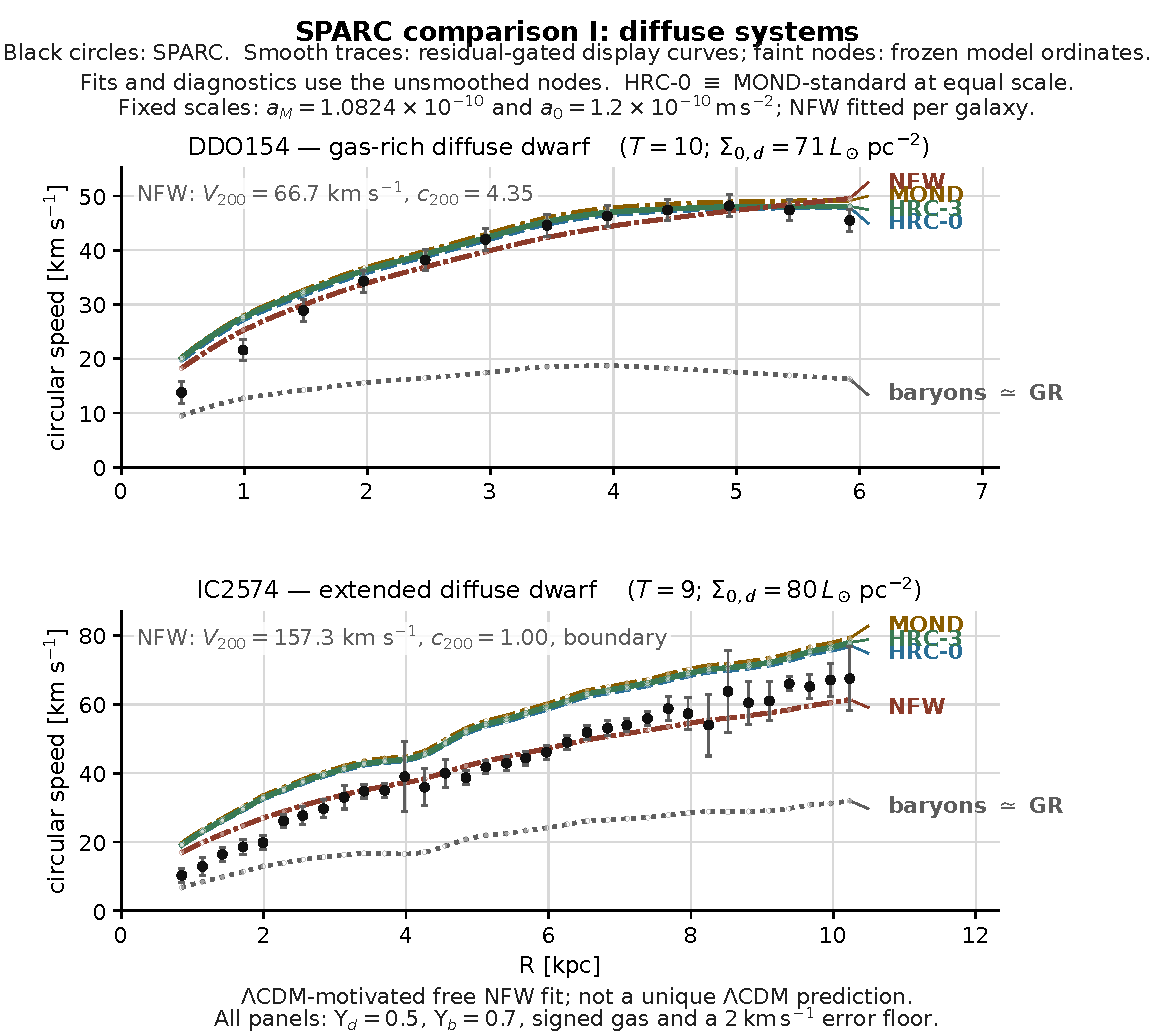
\includegraphics[width=\textwidth]{../figures/r154/curve_semantics/main/R154_SPARC_SMOOTH_DISPLAY_A.pdf}
\caption{Representative SPARC external comparison, set~I: DDO~154 and
IC~2574.  Fixed baryonic
inputs are compared with baryon-only weak-field GR, MOND-standard, HRC-0,
conditional HRC-3 and a separately fitted two-parameter NFW halo.  HRC-0 and
MOND-standard have the same response shape at equal scale.  The NFW curve is
a $\Lambda$CDM-motivated free NFW fit, fitted to the displayed rotation
curve; it is not a unique $\Lambda$CDM prediction and not a population
model-selection result.  This is a Level-C local algebraic diagnostic, not a
population likelihood.  SPARC measurements are unconnected error-bar
markers, and source model ordinates are faint, unconnected nodes.  Smooth
traces are residual-gated, shape-preserving display approximations through
curvature-regularised display nodes; the maximum node-displacement tolerance
is \(0.10\)--\(0.25\,\mathrm{km\,s^{-1}}\).  All fit and diagnostic metrics
use the original nodes, and no continuous physical owner is implied.}
\label{fig:pop_sparc}
\end{figure}

\begin{figure}[p]
\centering
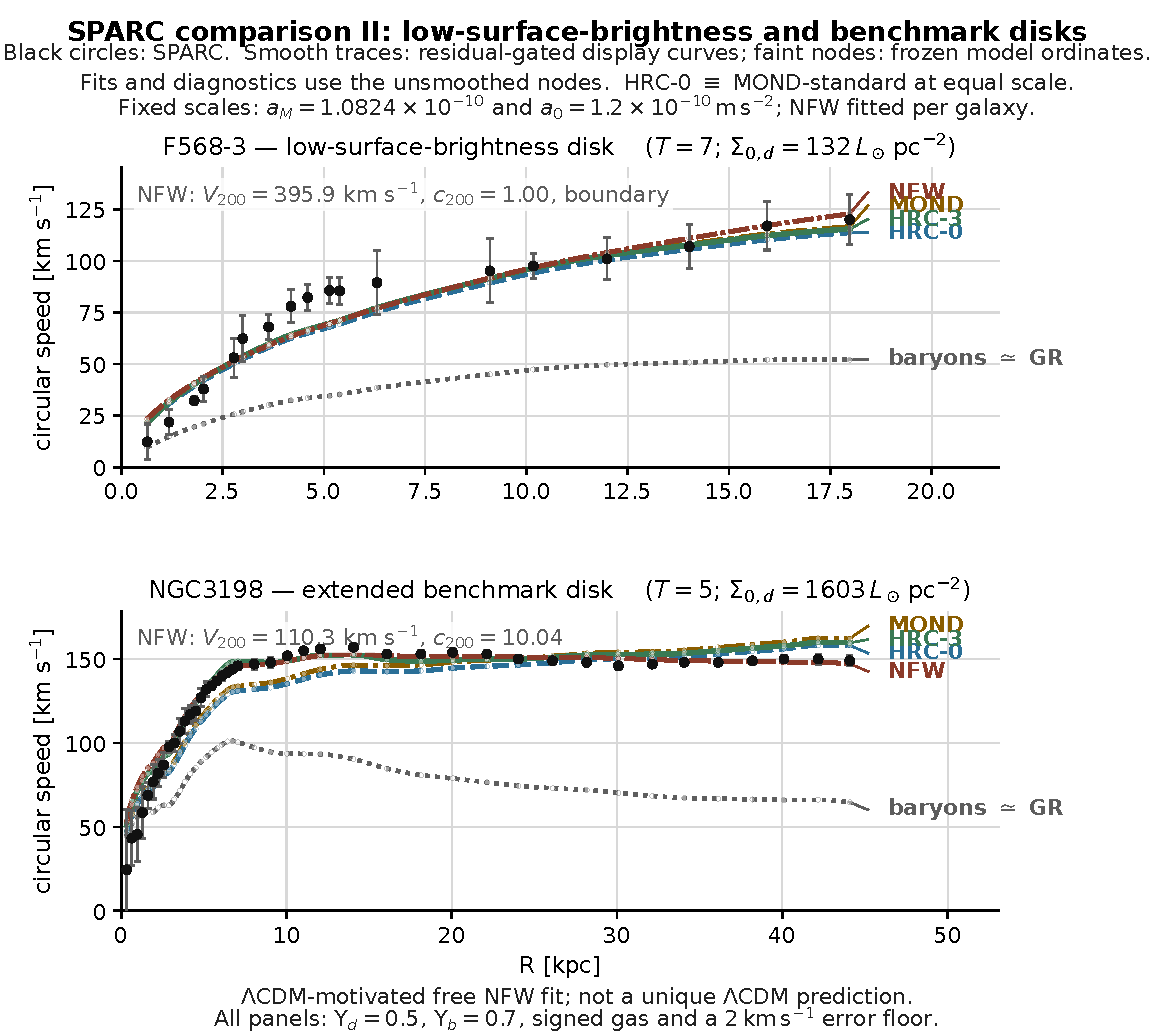
\includegraphics[width=\textwidth]{../figures/r154/curve_semantics/main/R154_SPARC_SMOOTH_DISPLAY_B.pdf}
\caption{Representative SPARC external comparison, set~II: F568--3 and
NGC~3198, with the same fixed baryonic inputs and status guards as
Fig.~\ref{fig:pop_sparc}.  The separately fitted NFW curve is a
$\Lambda$CDM-motivated free NFW fit; it is not a unique $\Lambda$CDM
prediction and not a population model-selection result.  The
reference-ordered technical-preprint appendix \emph{Visual atlas:
HRC diagnostics and rotation comparisons} keeps held-out, frozen
acceleration-stratified and post-hoc residual-stress families separate; none
is a survey-level comparison or ECT-discrimination result.}
\label{fig:pop_sparc_external_b}
\end{figure}

\begin{figure}[p]
\centering
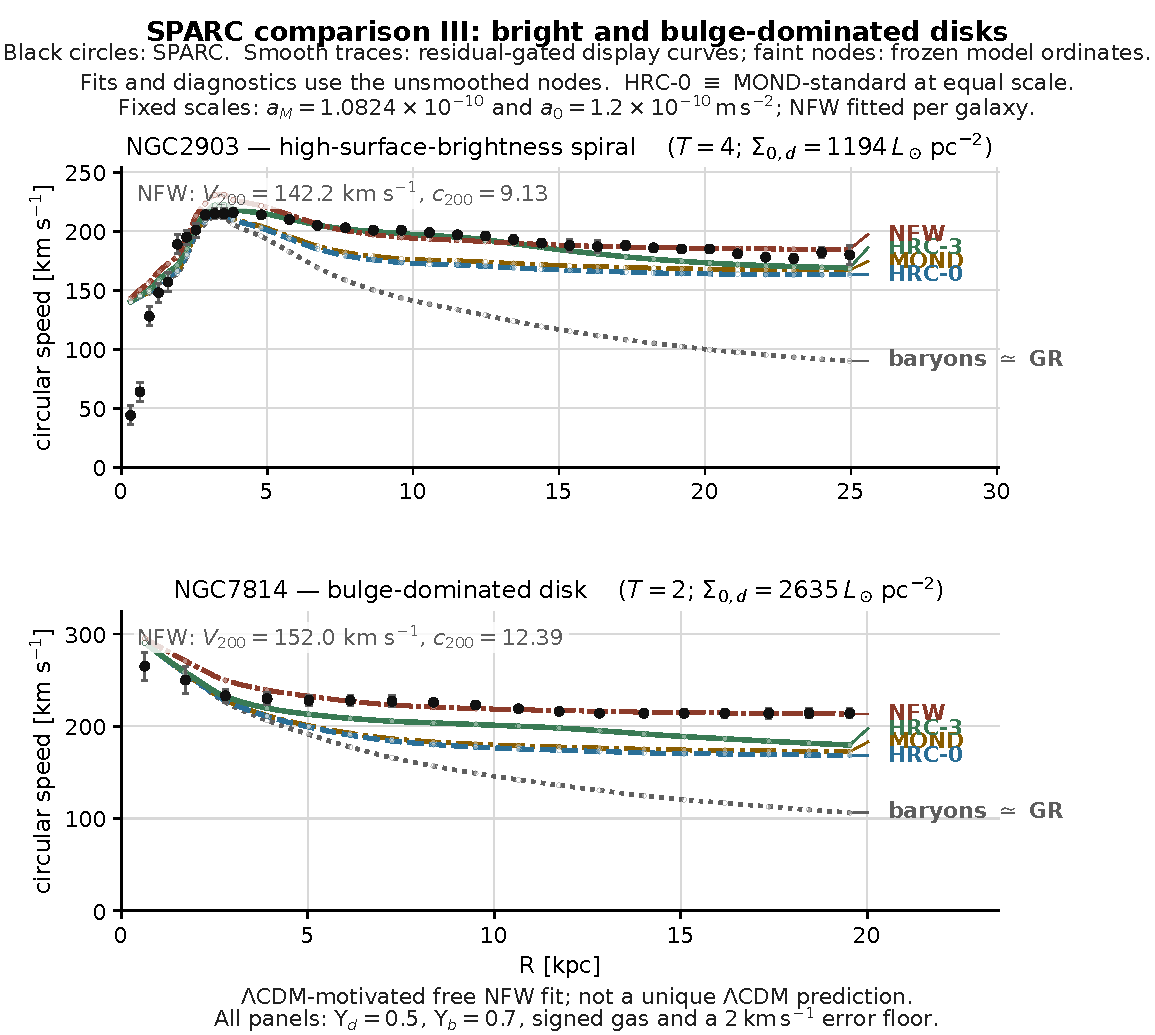
\includegraphics[width=\textwidth]{../figures/r154/curve_semantics/main/R154_SPARC_SMOOTH_DISPLAY_C.pdf}
\caption{Representative SPARC external comparison, set~III: NGC~2903 and
NGC~7814.  The five displayed curves use the same frozen fixed-baryonic
inputs and status guards as Fig.~\ref{fig:pop_sparc}.  The separately fitted
NFW curve is a $\Lambda$CDM-motivated free NFW fit, fitted to the displayed
rotation curve; it is not a unique $\Lambda$CDM prediction and not a
population model-selection result.  Together, the three companion figures
provide reader-scale views of the six-galaxy external-comparison owner
without upgrading this Level-C diagnostic to a survey likelihood.}
\label{fig:pop_sparc_external_c}
\end{figure}
\FloatBarrier

\par\noindent The frozen algebraic registry uses 165 SPARC galaxies, signed
gas and five repeated whole-galaxy held-out folds.  Its absolute statistics
are
\begin{center}
\small
\begin{tabular}{@{}lrrr@{}}
\toprule
Response & fixed-$M/L$ $\langle\chi^2\rangle$ & fixed-$M/L$ SD &
common-$M/L$ $\langle\chi^2\rangle$\\
\midrule
HRC-0 & 117598.72 & 3645.86 & 109439.95\\
HRC-3 & 99501.19 & 2967.18 & 103763.46\\
\bottomrule
\end{tabular}
\end{center}
The fixed-$M/L$ fits use 3343 points per seed; the common-$M/L$ mode
uses 3342.  Thus the absolute scale is approximately
$\chi^2/{\rm point}\sim30$, which is \emph{not} an acceptable survey
likelihood.  The calculation omits covariance, intrinsic scatter, distance
and inclination marginalisation, hierarchical stellar populations, the disk
curl field and the external-field response.  These results are Level~C
diagnostics, not ECT-specific evidence.  They show that HRC can be evaluated
consistently, but not that the galactic sector is closed.

\paragraph{How to read the rotation-curve lines.}
Every baryonic, MOND/HRC or NFW source ordinate is evaluated at
the corresponding tabulated SPARC radius and retained as a faint, unconnected
node.  The coloured traces are residual-gated, shape-preserving display
approximations through curvature-regularised display nodes.  This presentation
step is not a second physical or statistical fit: all fitted parameters,
likelihoods, residuals and diagnostic metrics use the original frozen
ordinates.

\par\noindent\textit{Reader guide.}  The three preceding pages are one
six-galaxy fixed-baryonic external-comparison sequence.  They retain the
Level-C local-diagnostic status stated above and are not a survey-level or
population-model-selection result.  The complete reference-ordered visual
atlas remains in the technical preprint.

For a declared exponential Milky-Way disk and 14 representative velocity
points, the HRC sensitivity calculation gives
\begin{equation}
\begin{array}{c|cc}
 & a_M/a_{M0} & \chi^2_{\rm red}\\ \hline
\mathrm{HRC\!\!-0} & 2.798 & 1.813\\
\mathrm{HRC\!\!-3} & 1.703 & 2.287
\end{array}.
\label{eq:pop_hrc_mw}
\end{equation}
This is not a modern Milky-Way posterior: gas, bulge, correlated systematics
and baryonic-model uncertainty are absent.

\begin{figure}[H]
\centering
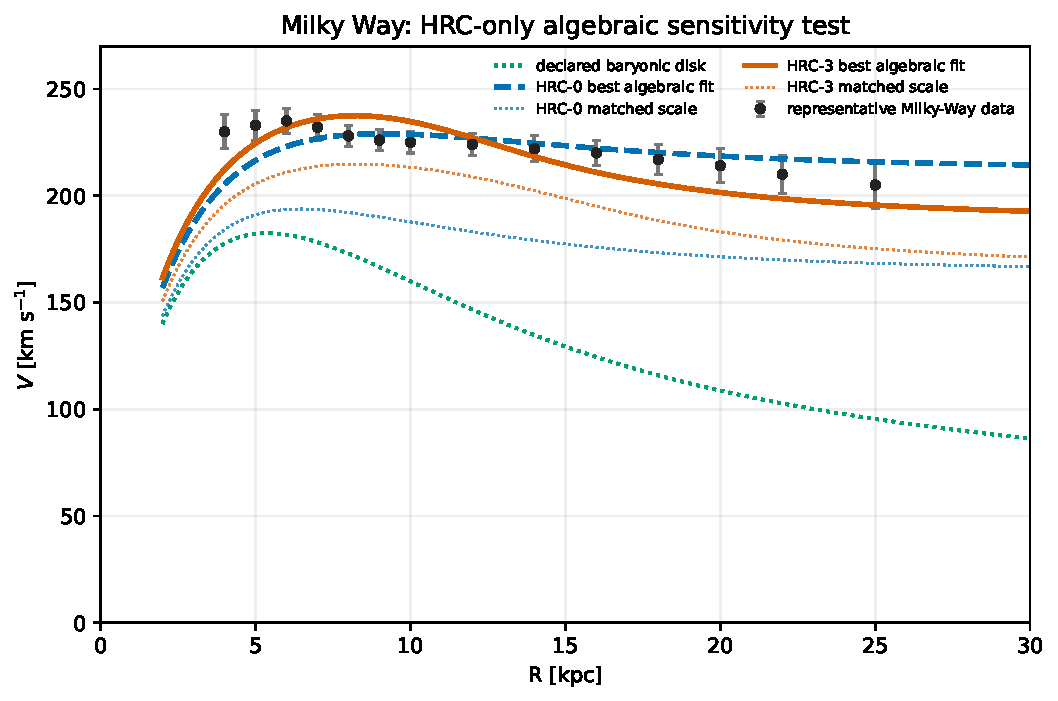
\includegraphics[width=0.88\textwidth]{hrc/R97_HRC_MILKY_WAY.pdf}
\caption{Representative Milky-Way HRC sensitivity test. Dotted curves use
the matched scale; solid/dashed curves use the best-fit scale for the declared
exponential disk. This is not a joint Milky-Way posterior.}
\label{fig:pop_mw}
\end{figure}

\section{The baryonic Tully--Fisher relation, RAR, and UDG stress test}

Both HRC responses share $\mu_g\sim g/a_M$ in the deep branch.  For an
isolated spherical source, conditional on the separate gravity bridge,
\begin{equation}
 g^2\simeq g_Na_M,\qquad
 v_{\rm flat}^4=G_NM_ba_M.
 \label{eq:pop_hrc_btfr}
\end{equation}
The slope~4 is therefore Level~A algebra inside the supplied static
functional and Level~B/Open after the bridge.  Its normalisation and scatter
are observational questions and do not identify a microscopic owner for
$a_M$.

\begin{figure}[p]
\centering
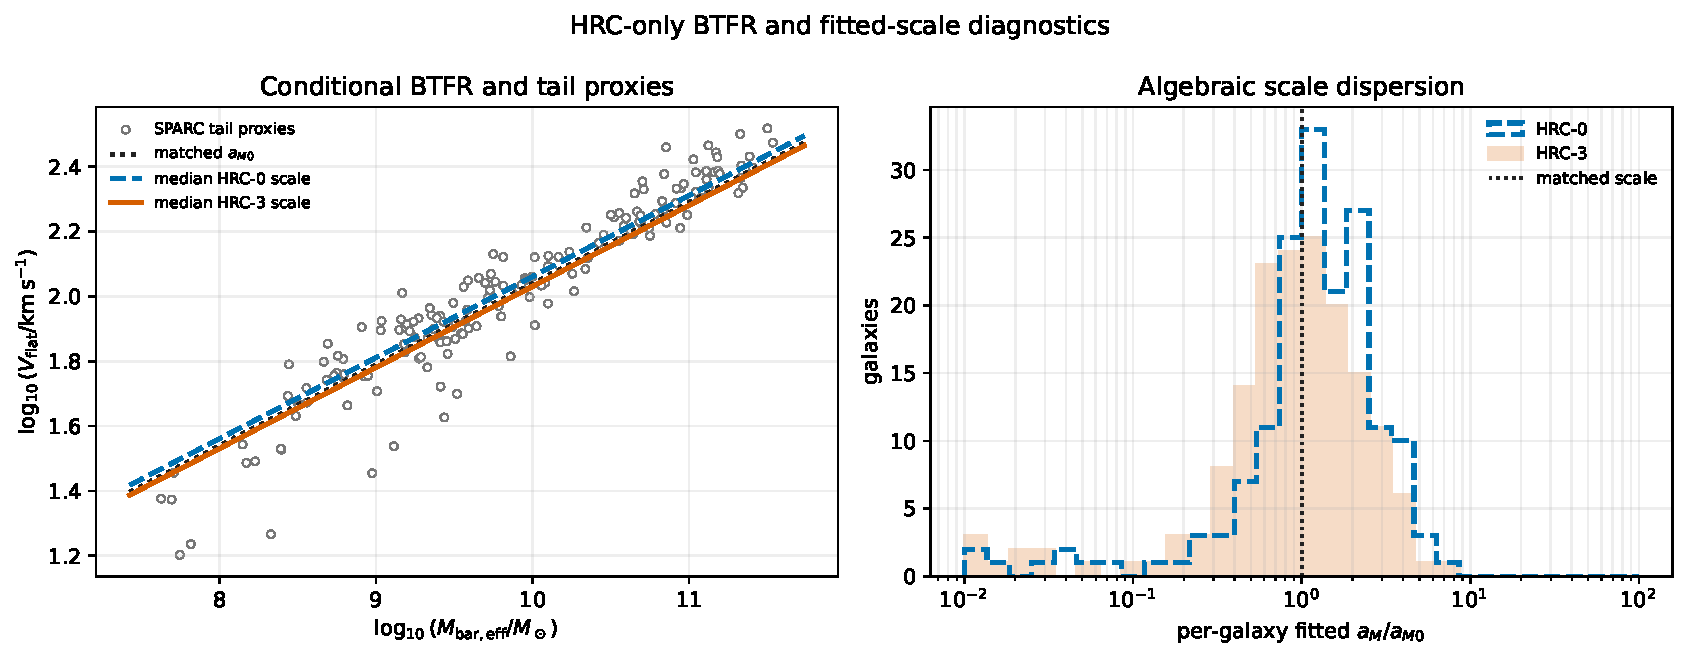
\includegraphics[width=0.98\textwidth,trim=0 0 405.012bp 26bp,clip]{hrc/R97_HRC_BTFR_AND_SCALE.pdf}
\caption{Conditional BTFR proxies in the HRC-only diagnostic.  The slope-four
lines are conditional on the identity gravity bridge; the mass proxy is taken
from the same SPARC decomposition and is not an independent catalogue
likelihood.  This is the enlarged frozen left panel; no mass proxy or line has
changed.}
\label{fig:pop_btfr}
\end{figure}
\begin{figure}[p]
\centering
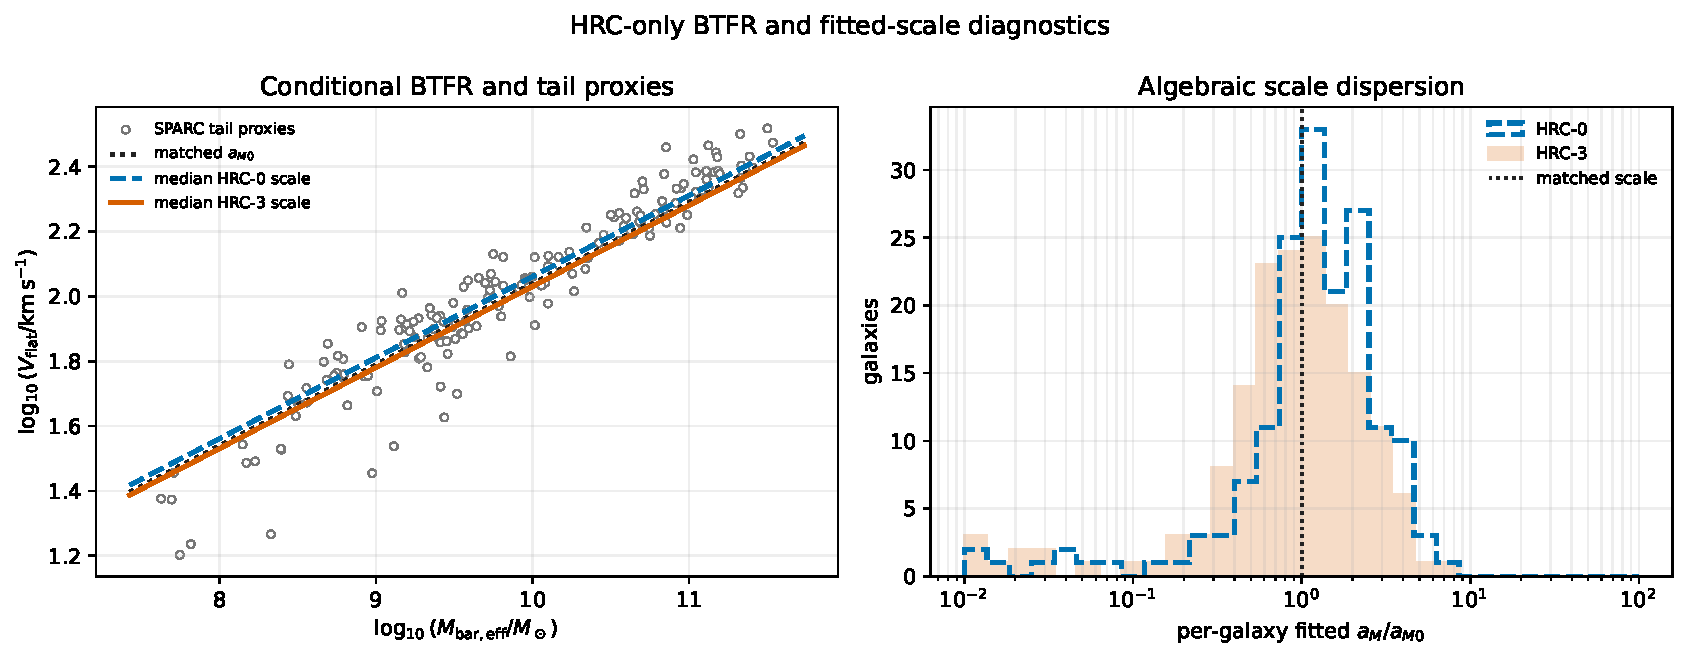
\includegraphics[width=0.98\textwidth,trim=405.012bp 0 0 26bp,clip]{hrc/R97_HRC_BTFR_AND_SCALE.pdf}
\caption*{\textbf{Continuation of Fig.~\ref{fig:pop_btfr}: fitted-scale
dispersion.}  This is the enlarged frozen right panel; no fitted value or bin
has changed.}
\end{figure}
\FloatBarrier

The symmetry-reduced RAR diagnostic solves
\begin{equation}
 g_N=\mu_{g,k}(g_{\rm obs}^2/a_M^2)g_{\rm obs},
 \qquad k\in\{0,3\}.
 \label{eq:pop_hrc_rar}
\end{equation}
For a generic disk this local relation omits the curl field in
$\mu\boldsymbol g=\boldsymbol g_N+\boldsymbol\nabla\times\boldsymbol H$.
Consequently the RAR plot is a pipeline diagnostic, not an independent
prediction of P1--P6.

\begin{figure}[H]
\centering
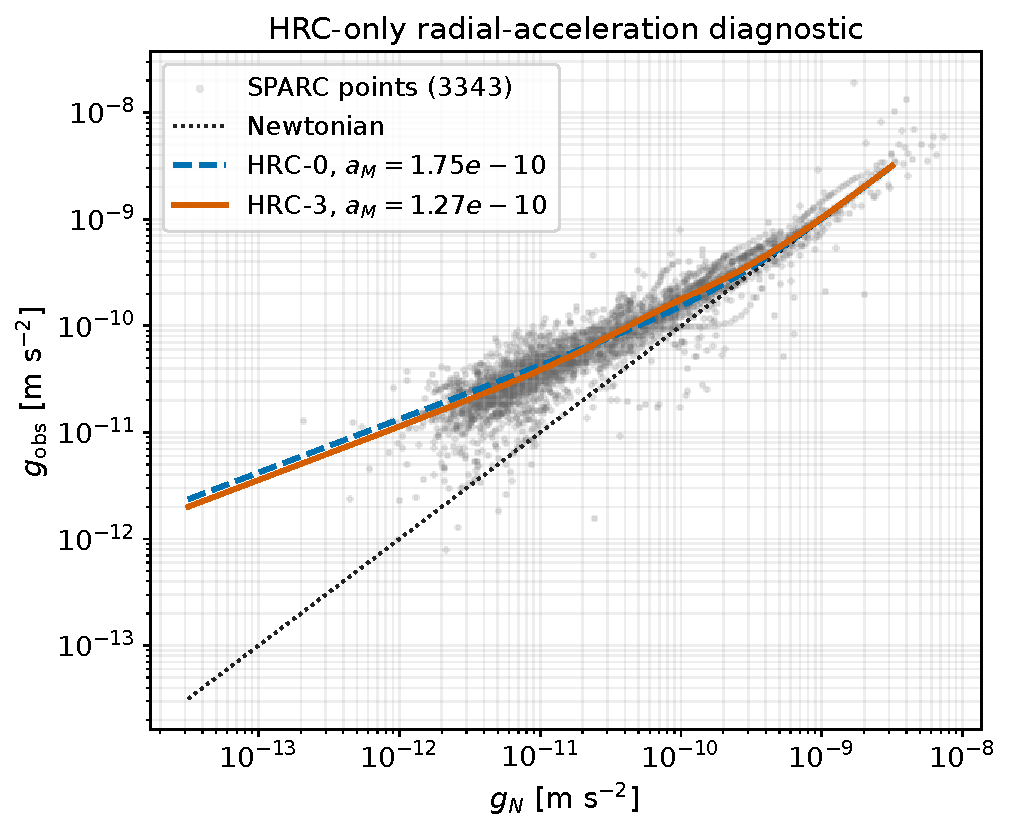
\includegraphics[width=\textwidth]{../figures/r149/R97_HRC_RAR_DIAGNOSTIC_typography_r149.pdf}
\caption{HRC-only RAR diagnostic for 3343 SPARC entries.  The curves use the
mean held-out fitted scales of the frozen local algebraic pipeline; covariance
and the full disk field are absent.}
\label{fig:pop_rar}
\end{figure}

For pressure-supported ultra-diffuse galaxies define
$\mathcal R_{\rm dyn}=g_{\rm obs}/g_N$.  A positive HRC enhancement exists
only for $\mathcal R_{\rm dyn}>1$.  HRC-0 gives
\begin{equation}
 \frac{a_M^{(0)}}{g_{\rm obs}}=
 \sqrt{\mathcal R_{\rm dyn}^2-1},
 \label{eq:pop_hrc_udg}
\end{equation}
and HRC-3 is inverted by monotone bracketing.  Central Wolf-proxy values give:
DF4, no positive solution; FCC~224,
$a_M^{(0)}/a_{M0}=0.0155$ and $a_M^{(3)}/a_{M0}=0.00780$;
DF2, $0.0476$--$0.470$ and $0.0278$--$0.457$;
NGC~5846-UDG1, $0.947$ and $0.935$; Dragonfly~44, $4.951$ and
$4.944$.  These heterogeneous central proxies are not a common-confidence
Jeans sample and do not establish an environment law.

\begin{figure}[H]
\centering
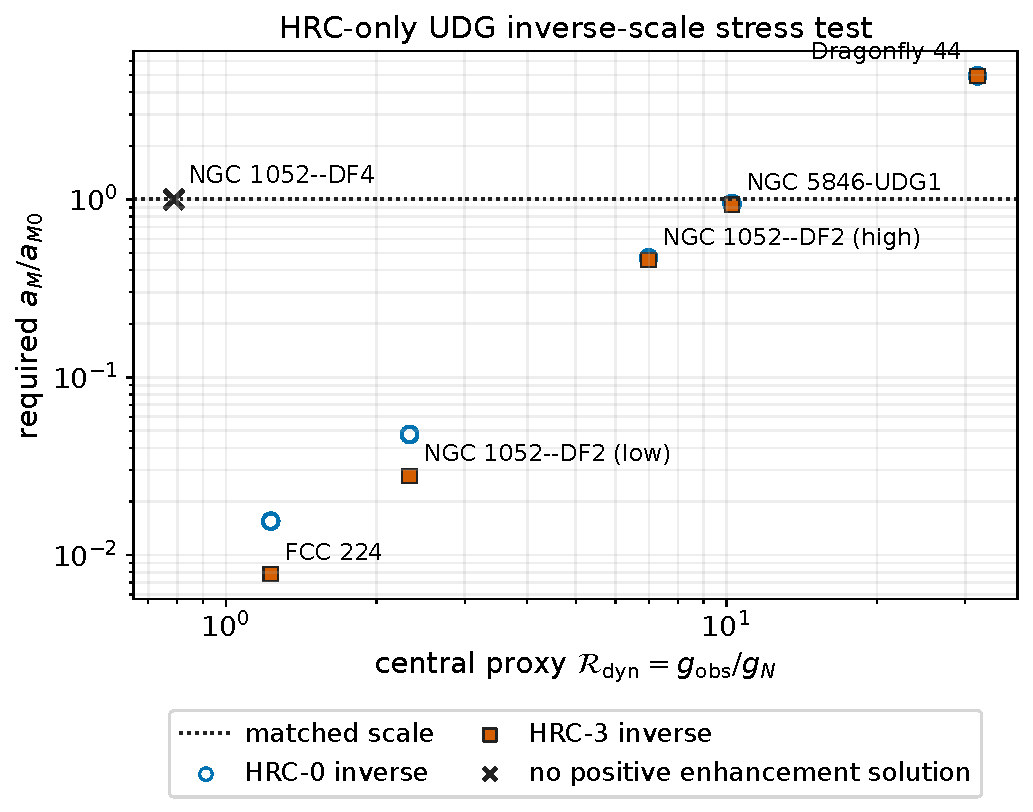
\includegraphics[width=\textwidth]{../figures/r149/R97_HRC_UDG_STRESS_typography_r149.pdf}
\caption{HRC-only inverse-scale UDG stress test.  The cross marks a central
proxy outside the positive-enhancement domain.  The matched-scale line is not
an environment fit.}
\label{fig:pop_udg_regime}
\label{fig:pop_udg}
\end{figure}

\FloatBarrier

\section{Audit of the projected cluster proxy}
\label{sec:pop_clusters}

The existing cluster script is not a physical HRC cluster solver.  It applies
a local surface-density map paired with the conditional HRC-0 point-source
response to hand-set baryonic maps.  For any strictly increasing positive
local map, preservation of ordering and of the possibly empty set-valued
total-map argmax is a Level-A theorem inside that supplied map.  Whenever
peaks are attained, the transformed maximizers equal the input maximizers.
No synthetic replay or finite-box amplitude
is retained as active phenomenology.  The physical matter source, response
kernel, photon metric, retarded collision dynamics and observational map are
Open.  Hence the identity does not explain residual cluster mass, lensing
amplitude or Bullet-like offsets; those require independently constrained
baryonic maps, a nonspherical dynamical solution and a prespecified joint
lensing likelihood.

More explicitly, the retained proxy uses
\begin{equation}
 \Sigma_{\rm cl}=\Sigma_b\nu_{\rm cl}
 \!\left(\frac{2\pi G_N\Sigma_b}{a_{M,\rm cl}}\right),
 \qquad
 \nu_{\rm cl}(y)=
 \sqrt{\frac{1+\sqrt{1+4/y^2}}{2}}.
 \label{eq:pop_cluster_hrc0_proxy}
\end{equation}
Because $d[\Sigma_b\nu_{\rm cl}(K\Sigma_b)]/d\Sigma_b>0$ throughout the
positive value interval, the transformed and input maps have the same
set-valued argmax.  Whenever peaks are attained, their maximizer sets
coincide.  This exact identity is why peak agreement is not morphology
evidence.

\paragraph{Restricted transport no-go and figure status.}
The local-map theorem cannot generate a collision offset.  Independently, if
one assumes one constant real Debye pole,
$\tau_{\rm pole}=2\pi/H_0$, together with ballistic transport
$\ell=v\tau_{\rm pole}$, the static matching time is about three orders of
magnitude longer than the $70$--$100$~kpc merger-lag time.  This is a
conditional Level-A no-go only for that joint one-pole/ballistic model; a
multi-pole, dispersive, non-ballistic or separately owned causal kernel
remains Open.  A physical cluster figure still requires an action-owned
retarded collision and lensing calculation; no hand-set proxy map is
presented as a physical cluster model.

\section{Matter--antimatter asymmetry}

The observable universe contains far more matter than antimatter:
$\eta_B^{\rm obs}\approx6\times10^{-10}$.  A conventional dynamical
baryogenesis mechanism requires baryon-number violation, $C$/$CP$ violation
and departure from thermal equilibrium.  The Standard Model contains
sphaleron processes and CP violation, but with the measured parameters it
does not supply sufficient CP and out-of-equilibrium dynamics to reproduce
the observed asymmetry.

P4 supplies an ordered branch, but not a derived real-time transition or
nonequilibrium state.  Topology does not define physical baryon number, and
the director term does not supply a nonzero CP coefficient, baryon-violating
vertex, transport or washout.  The observed $\eta_B$ is therefore an external
target for an Open completion programme, not an ECT result.  No imported
thermal-leptogenesis parameter tuple is retained as ECT phenomenology.





\section{Conclusions of Part~II}

\subsection{Status-separated outputs, benchmarks, and Open targets}

The current preprint records the following geometric-branch results and closure benchmarks:

\begin{enumerate}
\item Lorentzian kinematics as the homogeneous limit of the scalar/phase characteristic model (\emph{A inside that model}); physical special relativity requires the clocks/rods, matter, and photon maps (B/Open).
\item Scalar-only metric normalization derived inside its ansatz; an orientation stress $T^{(n)}_{\mu\nu}$ requires a covariant $S_n[g,n,\lambda_n]$ and remains Open.
\item Structural or conditional non-inflationary routes to horizon-scale
homogeneity and a flat baseline branch, plus the A-math conditional statement
$\pi_2(S^3)=0$ for the supplied orientation target and an
exact flat \emph{formal local seed} only in a supplied pure-quartic kernel;
the physical vacuum manifold, relic conclusion, finite band, state, transfer
and observed primordial spectrum remain Open.
\item Late-time acceleration and $w(a)$ require an action-owned stable background and joint likelihood (Open).
\item Cosmological background and age: one supplied two-slope action and legitimate state datum give conditional $H(z)$, distances, high-redshift times and $\tau_{2s}\equiv H_{2s}(0)\Delta t=0.96368678$; a dimensional age additionally uses one declared calibration. Whether microscopic $\Phi$ dynamics constrains this completion, and the physical metric/redshift/lapse/front/congruence map, remain Open.
\item JWST abundance and morphology require an end-to-end background, perturbation, halo, baryonic and selection forward model (Open).
\item 165 SPARC galaxies: HRC-only held-out totals are disclosed with an absolute scale $\chi^2/{\rm point}\sim30$; this is a Level-C stress diagnostic, not a precision fit.
\item BTFR slope exactly 4 conditional on the adopted deep-branch closure (\emph{B/C}).
\item RAR fit with $a_M \approx cH_0/(2\pi)$ (\emph{C}); the physical matching and environment law are Open.
\item Strictly increasing local-map order/argmax theorem (Level~A inside the supplied map); no active synthetic replay or finite-box amplitude; physical source, metric, retarded collision and lensing map Open.  One constant real Debye pole with $\tau_{\rm pole}=2\pi/H_0$ plus ballistic transport is conditionally excluded, while general causal kernels remain Open.
\item Baryogenesis: only an external observational target and an Open
completion inventory are available; no real-time transition, baryon current/vertex,
CP coefficient, transport, washout or ECT-native $\eta_B$ is derived.
\item A Level-C no-halo galactic fit and a separate calibrated late-time scalar closure; their ECT matching, particle content, and common microscopic origin remain Open.
\end{enumerate}

\subsection{Key equations and principles of Part~II}

Scalar-only metric equation (undivided): $F G_{\mu\nu}=8\pi G_N T_{\mu\nu}/c^4+\mathcal T^{(q)}_{\mu\nu}$; division by $F$ introduces no orientation term, and $T^{(n)}_{\mu\nu}$ requires a separate covariant $S_n[g,n,\lambda_n]$ (Open).

HRC algebraic relation: $g_N=\mu_{g,k}(g^2/a_M^2)g$, $k\in\{0,3\}$.

BTFR: $v_{\rm flat}^4 = G_N M_{\rm bar} a_M$ (slope 4, algebraic).

$t_{0,\rm ECT}=\int_{a_{\rm ord}}^1 da/[aH_{\rm ECT}(a)]$; the named two-slope state gives $\tau_{2s}\equiv H_{2s}(0)\Delta t=0.96368678$ conditionally. Only after declaring $H_{2s}(0)=H_0^{\rm cal}$ may this be written as $H_0^{\rm cal}t_0$; the physical observable map and microscopic selection remain Open.

\subsection{Conditional completion tests and external observational gates}

The macroscopic sector currently supplies a mixed set of conditional
closure tests, fitted diagnostics, external observational gates and Open
programmes.  These items are not uniformly ECT predictions:

\begin{itemize}
\item BTFR slope = 4 conditional on the adopted galactic closure (\emph{B/C}); fitted $a_M \sim cH_0/(2\pi)$ (\emph{C}).
\item The homogeneous director-vector term has no spin splitting and no source-generated E\"otv\"os force; external spin/WEP data constrain only separately declared completions.  The physical late-time source and $w(a)$ remain Open.
\item Exploratory environment/history law $\Xi$ (\emph{Open}); physical tensor polarisation and graviton mass remain Open, with two TT modes only in a supplied massless Fierz--Pauli completion.
\end{itemize}
The full status-separated list is given in Part~V,
Section~\ref{sec:pop_predictions}.

Figure~\ref{fig:pop_r114_early_response_envelope} now visualises a frozen five-row sensitivity envelope; it is deliberately not called a cosmological prediction.  A genuine prediction image remains deferred until one exact ECT background and observable pipeline passes all closure gates.

\subsection{Part~II status and dependency logic}

\begin{figure}[H]
\caption{Complete connected Part~II status and dependency map. The supplied ordered-branch EFT,
conditional macroscopic completions, owner-specific cosmology gates and Open
targets are kept distinct. The routes separate the exact orientation determinant,
conditional trace-free $V+C_I$ and two-slope results, and the Open physical
ECT action/state/metric map.  All canonical nodes and edges appear in one
colour-coded A4 reader map; arrows do not certify derivation.  The
deterministic exact-key and machine-topology records preserve the canonical
source labels and edge inventory.}
\label{fig:pop_partII_logic}
\end{figure}

The status and dependency logic of Part~II is shown in
Fig.~\ref{fig:pop_partII_logic}.  It is deliberately kept whole so that the
gravity, cosmology, galactic and vacuum-offset branches remain visibly
connected.  The PDF is vector content for reader zooming; no edge upgrades
the literal status of either endpoint.  It explicitly marks $F$ as supplied,
limits $w_{\rm bare}\ge-1$ to the bare positive-kinetic ratio, preserves the
false observable-$w_{\rm eff}$ implication as a blocked edge, separates the
GR-reference density conversion from the Open scalar--tensor late source, and
restricts the JWST result to the nine computed nodes.

\clearpage
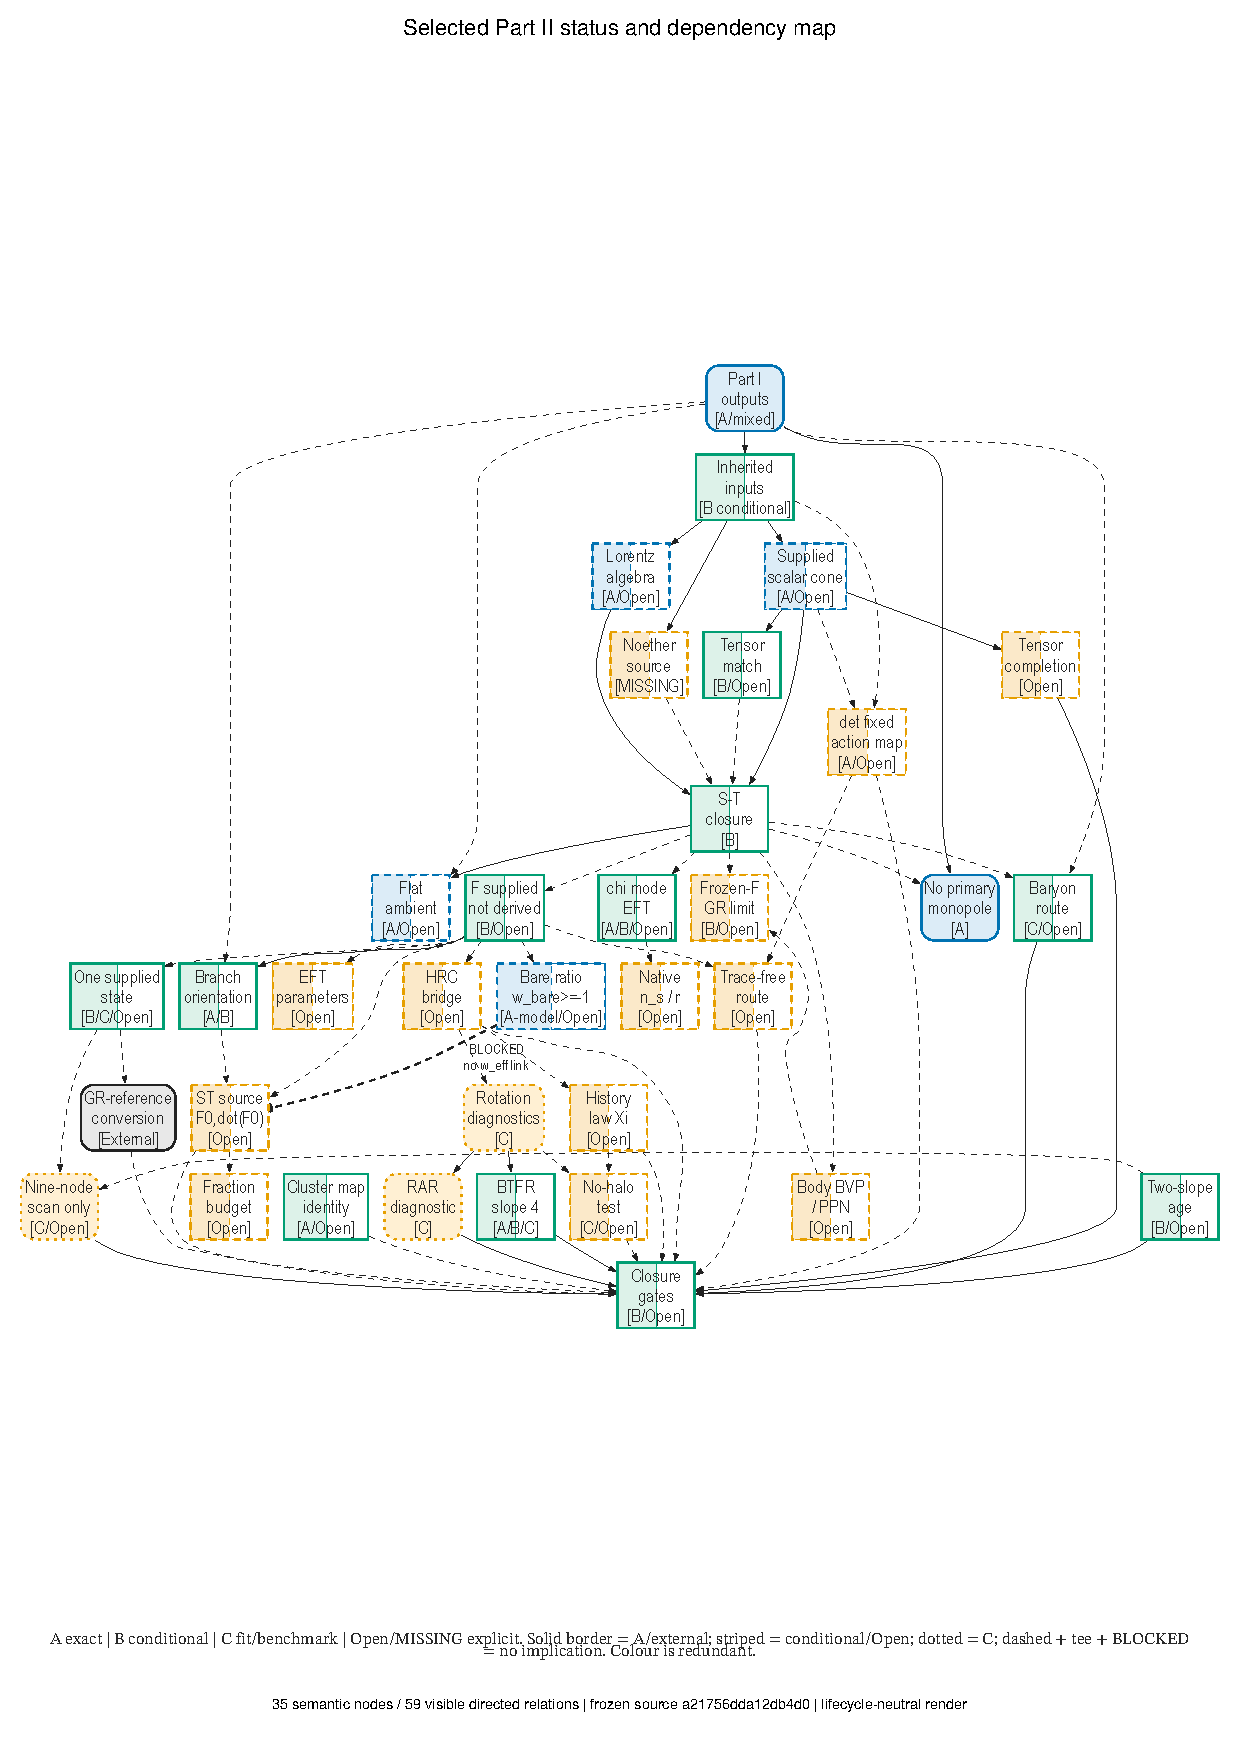
\includepdf[
  pages=1,
  fitpaper=true,
  pagecommand={\thispagestyle{empty}}
]{../figures/r185/logic_maps/partII_status_dependency.pdf}
\clearpage

%==============================================================
\part{Quantum Sector: Coherent Branch}
\label{part:quantum_pop}

\noindent\textbf{Why does quantum mechanics exist?} In ECT, the answer has three layers.

\emph{First}: the Euclidean functional integral. Because the
fundamental arena is a four-dimensional Euclidean manifold with no built-in
time, the P3 model distinguishes the dimensionless reduced functional
$\mathcal I_E^{\rm P3}$ from the physical classical action
$S_E^{{\rm P3},{\rm phys}}=A_{\rm P3}\mathcal I_E^{\rm P3}$, where
$A_{\rm P3}>0$.  A separately supplied P3 measure has the weight
$\exp[-\kappa_{\rm P3}\mathcal I_E^{\rm P3}]
=\exp[-S_E^{{\rm P3},{\rm phys}}/\Sigma_{\rm PI,P3}]$, with
$\Sigma_{\rm PI,P3}>0$ and
$\kappa_{\rm P3}=A_{\rm P3}/\Sigma_{\rm PI,P3}>0$.  Neither action scale,
their ratio, nor a map to $S_0$, $\Sigma_\theta$, $\Sigma_\vartheta$ or
$\hbar$ is derived; $\kappa_{\rm P3}=1$ would be only an explicit
normalisation convention.  These action symbols are also unrelated to the
protocol entropy production $\Sigma[\gamma]$.  The integral sums over
all field configurations, including ``closed histories'' where the field
returns to itself along the fourth coordinate; there are no events, temporal
ordering or cause--effect sequences at this level.  For supplied
Gaussian/free kernels satisfying the complete applicable corrected OS-II
hypothesis package, the positive-semidefinite form can be quotiented by its
null space and completed to a conditional Hilbert-space reconstruction.  The
declared checks establish only their specified kernels; the interacting ECT
measure, observable algebra, continuation and generator, physical
clock/metric and theory-wide unitarity remain B/Open.

There is one useful same-channel closure gate.  For a supplied positive free
mode in the infinite-time vacuum, if the OS and canonical descriptions use
the same normalised $q$, calibrated $m,\omega$ and pole residue, with no
field/source renormalisation, their full correlators are respectively
$\Sigma_{\rm PI,ch}e^{-\omega|\tau|}/(2m\omega)$ and
$S_{0,{\rm ch}}e^{-\omega|\tau|}/(2m\omega)$.  Equality for that same channel
forces $\Sigma_{\rm PI,ch}=S_{0,{\rm ch}}$.  This is standard conditional
free-mode mathematics and a B/Open ECT consistency gate, not a P3
identification, $A_{\rm P3}=\Sigma_{\rm PI,P3}$, cross-sector universality or
a derivation of $S_0=\hbar$.  Field/residue maps, finite temperature,
interactions, constraints or non-vacuum states require a new comparison.

\emph{Second}: supplied action-scale candidates and their possible match to $\hbar$. After BR1 supplies a compact complex field, single-valuedness gives $\oint \partial_A\theta\,dX^A = 2\pi n$, while a phase-only fixed-core closure defines $\iota_{\rm elem}^{\rm(fixed\ core)}=2\pi \iota_0^{\rm EFT}$.  CDE-$\Phi$ is only a post-order acceptance criterion.  A distinct reparametrisation-invariant texture-worldline route defines $\iota_{0,\rm bal}^{(\vartheta)}=\sqrt{2K_\vartheta^{1\mathrm D}\mathcal T_{\rm loop}}$ only after a 4D owner supplies the carrier, compact modulus and proper-time ensemble.  Under the separate bending-free $n=1$ matching this gives $\Sigma_\vartheta\mathcal I_{1,\min}=2\pi\hbar=h_{\rm P}$; the relation is physically motivated but does not derive the measured value.  Profile/Hessian, bending/barrier and cross-sector universality remain Open (\emph{Level-A reduced algebra / Level-B route / Open ownership and matching}).

\emph{Third}: reduced-state records.  A declared environment can suppress
interference between specified alternatives, but the pairwise record exponent
does not create Lorentzian signature, define a universal
quantum--classical boundary, or select one realised outcome.  Deriving the ECT
record operators, state, and detector update remains Open.

\section{ECT versus standard quantum mechanics}
\label{sec:pop_ect_vs_qm}

Standard quantum mechanics supplies a tested operator and probability
framework. ECT offers reconstruction routes from selected Euclidean coherent
subsectors, but their statuses differ: the quadratic RP/OS bridge is controlled,
whereas interacting states, Born weights without a supplied physical probability owner and the complete representation-theorem hypotheses, detector updates, and
solution-selection measures remain B/Open.  A Euclidean boundary-value
formulation is therefore an architectural hypothesis, not a proof that quantum
probability is merely coarse-graining or that one unique global solution exists.

\subsection{Detailed structural comparison: ECT vs standard QM}

The following examples compare the ECT coherent-branch interpretation with
standard quantum mechanics in specific situations.  Each case states what the
standard formalism already predicts, what additional owners a future ECT
reconstruction would require, and the present status; no extra explanatory
success is assumed.

\paragraph{The hydrogen atom.}
The standard Coulomb boundary/eigenvalue problem yields discrete levels.  ECT
is compatible with embedding that effective problem in an ordered medium, but
compact winding is not a universal explanation of every discrete spectrum.
The Coulomb Hamiltonian, $-13.6/n^2$ levels, fine structure, Lamb shift,
hyperfine splitting, and $\alpha_{\rm fs}$ have not been derived from the
minimal ECT action (B/Open).

\paragraph{The double-slit experiment.}
Admissible Euclidean solutions or an ensemble of solutions may depend on the
declared apparatus boundary data.  ECT has not established uniqueness of that
nonlinear boundary-value problem, a physical measure over solutions, the map
to slit/detector settings, or the observed $|\psi_1+\psi_2|^2$ probabilities.
The global-boundary reading is interpretive compatibility (B/Open), not an
ECT-native derivation of the fringe pattern.

\paragraph{The Aharonov--Bohm effect.}
\begin{description}[leftmargin=2.8cm, style=nextline]
\item[Standard QM.] A charged particle acquires an observable phase shift $\Delta\varphi = (e/\hbar)\oint A_\mu\,dx^\mu$ even in regions where the electromagnetic field strength vanishes, provided the path encircles a non-trivial gauge flux.
\item[ECT (conditional picture).] The compact phase $\theta(X)$ can support a
winding label, but an electromagnetic holonomy follows only after a physical
Abelian connection and charged matter representation have been constructed.
\item[Required ECT owners.] A future ECT calculation would need an unbroken
$U(1)_{\rm em}$ connection, a charge/matter map, a candidate-to-operational
action owner, and the separately adopted Level-B calibration $S_0=\hbar$.
\item[Status.] Interpretive compatibility (\emph{B/Open}), not an ECT derivation of the electromagnetic AB phase.  The physical connection, charge and matter map remain Open.
\end{description}

\paragraph{Measurement and outcome selection.}
A specified influence-functional reduction can suppress interference and form
  stable records.  Pointer-basis selection, a single outcome, exact Born weights,
  and a detector update theorem are not established.  For a complex Hilbert space of dimension at least three, the ordinary projector Gleason theorem constrains only an already admitted normalized, noncontextual, countably additive probability measure on orthogonal projector decompositions to trace form.  In dimension two, ordinary projector Gleason does not apply.  Under the separately supplied condition C2q---a generalized measure $v$ on all effects $0\le E\le I$, with $0\le v(E)\le1$, $v(I)=1$, and $\sigma$-additivity for every countable effect sequence satisfying $\sum_iE_i\le I$ (a normalized POVM with $\sum_iE_i=I$ is the special case)---the Busch extension~\cite{Busch2003Gleason} may instead be applied; without C2q it may not.  Neither result creates probability or selects the prepared state.  The separate application condition C3 must also be supplied: a preparation together with a projector (ordinary C2) or an effect/POVM outcome (C2q) must be mapped to a laboratory event.  ECT has not derived the physical owner of that map; it remains Open.  Dephasing and record formation belong to a distinct application layer and are not theorem hypotheses.  The Hilbert/projector setting, measure assumptions and origin
  of probability therefore remain B/Open rather than following from bare
  P1--P6.

\paragraph{Conditional field-level determinism.}
The Euclidean field equation defines a classical nonlinear boundary-value
problem once a branch and admissible boundary data are specified.  Global
existence, uniqueness, stability, and a measure/selection rule over multiple
solutions have not been proved.  The no-fundamental-collapse ontology is an
architectural assumption; subsystem probabilities, Born weights, and the
measurement update retain their B/Open reconstruction status.  Thus ECT is
not presently a theorem that one boundary data set yields one unique global
configuration or that probability is absent at the deepest level.

\paragraph{Boundary dependence and delayed-choice compatibility.}
For a well-posed elliptic problem, interior solutions can depend on all
specified boundary data.  Mapping laboratory settings to ECT boundary data,
showing that later settings enter the physical problem, and reproducing
delayed-choice/eraser probabilities and no-signalling are all Open.  The
boundary-value picture is therefore an interpretive compatibility (B/Open),
not a derivation of future-setting influence or retrocausality.

\paragraph{Common-architecture hypothesis for the coherent and geometric branches.}
\begin{description}[leftmargin=2.8cm, style=nextline]
\item[Standard physics.] General relativity describes gravity; quantum mechanics describes microscopic coherence; how the two fit together is the canonical problem of quantum gravity.
\item[ECT (physical picture).] Both branches are organised within the same ordered-condensate architecture.  The controlled long-wavelength equation used here is scalar-only; a geometric orientation stress is a separate Open $S_n[g,n,\lambda_n]$ extension.  The shorter-wavelength coherent sector has a supplied local KG-form equation and a separately supplied complex law; only under the stated clock, positive-frequency, mass, interaction and slow-envelope assumptions does their leading NR relation admit a Schr\"odinger-type reading.
\item[What this suggests.] The common architecture makes a coupled gravity/coherent-sector completion conceivable.  A covariant orientation action, back-reaction vertex, and interacting quantum kernel are still required before quantitative back-reaction is claimed.
\item[Status.] The scalar mode decomposition is Level~A conditional
mathematics only inside the supplied scalar ansatz.  Its interpretation as
a common physical origin of tensor gravity and quantum dynamics is a
Level~B/Open architectural hypothesis; the common action, state,
back-reaction vertex and observable map remain Open.
\end{description}

\paragraph{What ECT conditionally organises rather than derives in full.}
\begin{enumerate}[label=(\roman*)]
\item A leading Schr\"odinger-type envelope as conditional asymptotic algebra after a norm-preserving complex law, Hamiltonian/domain, state/stable positive-frequency component, the same physical clock, mass matching, weak interaction, slow-envelope regime and residual control are supplied; the ordered real-scalar branch alone does not derive it;
\item the Klein--Gordon-form scalar sector after
      $d\tau=\mathcal N_\Phi dx^0/c_{\rm u}$.  The shorthand
      $t=\tau=w/c$ is restricted to an aligned planar branch with
      $\mathcal N_\Phi=1,c_{\rm u}=c$; independently, $\hat c_*$ fixes the
      scalar-cone slope;
\item the Robertson--Schr\"odinger inequality as exact mathematics only after a Hilbert space, self-adjoint domains and commutator are supplied; compact phase independently gives integer winding, while the physical commutator, finite-$S_0$ owner and cross-sector normalisation remain Open and $S_0=\hbar$ is the separate Level~B calibration;
\item reduced-state dephasing and record formation in specified channels; the ECT split, record operators, state, and kernels remain Open;
\item record formation without a metric-signature transition or unique-outcome theorem; pointer selection and update remain Open;
\item a conditional representation-theoretic route: the connected $SO(3)$
subgroup of the supplied $O(3)$ stabiliser has spin double cover
$\mathrm{Spin}(3)\simeq SU(2)$; identifying it with physical spatial
rotations and realising spinorial excitations remain Open, so this is not a
derivation of the physical spin sector;
\item the PES-R inventory of distinct stationarity, record, finite-time stability, and protocol diagnostics, without a universal selection theorem;
\item a programme for deriving an ECT gravitational record channel; the symbolic Di\'osi--Penrose comparator is external~\cite{Diosi1987,Penrose1996}, while the physical ECT vertex, state, and noise kernel remain Open;
\item separate tunnelling and entanglement owners; Euclidean connectivity supplies at most a geometric analogy, while a common dynamical mechanism remains Open;
\item a proposed cross-sector action-scale programme which must first derive the relation, if any, among $\iota_0^{\rm EFT}$, $\iota_{0,\rm bal}^{\rm eff}$ and the modulus-route $\iota_{0,\rm bal}^{(\vartheta)}$, and only then test whether one independently owned coefficient maps to a universal physical action normalisation; the four-dimensional owner, finite value, matching map and universality are not established.
\end{enumerate}

\paragraph{What remains open.}
The Born rule from first principles beyond the present closures; a completed detector channel, pointer basis, unique-outcome update, and ECT record kernel; Bell correlators directly from the condensate theory beyond toy visibility proxies; the detailed origin of three generations; the exact value of $\alpha_{\rm fs}=1/137$; the full Yukawa hierarchy.  These are presented as open derivational targets, not as failures of the framework.


\section{Conditional Hilbert-space reconstruction from the corrected OS-II package}

One central conditional route uses the corrected Osterwalder--Schrader reconstruction theorem.  Its input is not reflection positivity alone: one must supply Euclidean Schwinger functions or a measure, a physical observable algebra and time reflection, temperedness with the applicable OS-II regularity/growth condition, Euclidean covariance, reflection positivity, permutation or graded symmetry, and the applicable locality/cluster conditions.  The positive-semidefinite OS form is quotiented by its null space and completed to obtain the Hilbert space.  Gaussian/free checks establish only their explicitly verified kernels; the full interacting ECT measure, observables, continuation, generator, physical clock/metric map and $S_0$ identification remain B/Open.

The constructive Osterwalder--Schrader direction is from suitable Euclidean
Schwinger data to a Hilbert/Wightman description; Euclidean continuation of
an already supplied Lorentzian theory is the converse analytic route.  ECT
may use the constructive direction only where the complete applicable
corrected OS-II hypothesis set is verified.  This conditional mathematical
reconstruction does not by itself identify a physical ECT time, metric,
state, observable algebra or theory-wide unitary dynamics.


\section{Conditional spinor-compatibility route (physical spin Open)}
\label{sec:pop_spin}

In nonrelativistic quantum mechanics, spin transforms in $SU(2)$
representations of spatial rotations; in relativistic quantum field theory,
particle spin is classified through Poincar\'e representations and their
little groups.  Symmetry fixes the allowed representations, while which
representation a particle species realises is empirical input.

ECT offers a possible representation-theoretic backdrop, not a derivation
of physical fermions.  The connected Euclidean rotation subgroup is
$SO(4)$, whose spin double cover is
$Spin(4)\simeq SU(2)_L\times SU(2)_R$.  For the supplied nonzero P4 vector,
the full stabiliser is $O(3)$ and its connected $SO(3)$ subgroup has double
cover $Spin(3)\simeq SU(2)$.  These facts make spinorial representations
algebraically available.  Their identification with a physical
three-dimensional rotation group, and the physical metric/tetrad, spin
structure, matter action and stable excitation spectrum, remain Open.

On this reading, spin is not the literal mechanical rotation of a tiny ball in ordinary three-dimensional space.
Conditionally, it may be represented by a spinorial fermionic field compatible with the condensate symmetry structure.  A magnetic moment follows only after a physical fermion, an unbroken $U(1)_{\rm em}$, a matter vertex and its coefficient are supplied; it is not an output of rotational group theory alone.

\textbf{Important caveat.}
In the current formulation, fermions are introduced as fields compatible with the condensate symmetry, not yet derived as collective condensate excitations.
The electron $g$-factor, the fine-structure constant $\alpha_{\rm fs}$, and the hydrogenic fine structure are not yet calculated from condensate microdynamics.
These remain open derivational targets (\emph{Level~Open}).

\textbf{Superfluid analogy.}
A useful but limited analogy: in superfluid ${}^3$He-A~(Volovik 2003), Weyl fermions emerge as low-energy excitations near topological Fermi points---the spinorial character is a property of the quasiparticle spectrum, not an external input.
ECT does not yet reach this level of derivation for fermions.
The structural compatibility route developed in the main text should be understood as the present limit of what the framework can establish.
The superfluid example is an external existence example only.  It supplies
neither evidence for an ECT Fermi point nor an ECT spinor derivation.


\section{Superposition, interference, exchange statistics, and the Pauli exclusion principle}

\textbf{Linear superposition route} (\emph{A inside the quadratic subsector; B/Open physically}): solutions of the verified linearised equation can be added. Identifying this with the full interacting quantum-state principle requires the RP/OS and operator completion.

\textbf{Interference route} (\emph{Level~B route / Open physical ECT}):
after a quantum measure/coherent structure, composable kernel,
state/preparation and observable map are supplied, standard
constructive/destructive amplitudes can be represented.  Compact phase,
topology, linearity or elliptic boundary dependence alone derives neither the
quantum superposition rule nor arbitrary laboratory patterns.

\textbf{Indistinguishability of same-species particles} (\emph{Open physical owner}): membership in the same emergent mode sector does not by itself exclude unresolved core, orientation, internal or environmental labels.  If two physical ECT excitations are independently supplied as identical unlabeled point excitations in defect-free $\mathbb R^3$, the coordinate configuration space is the quotient by exchange used below.  ECT has not yet derived that excitation/identity map or excluded additional discrete fibres and sectors.

\textbf{Exchange statistics} (\emph{A topology conditional / Open physical statistics}): For
\[
 \mathcal M_2=((\mathbb R^3\times\mathbb R^3)\setminus\Delta)/S_2
\]
of two supplied identical point excitations in defect-free $\mathbb R^3$,
$\pi_1(\mathcal M_2)=\mathbb Z_2$ gives two homotopy classes.  Factors
$+1$ and $-1$ appear only after choosing the corresponding one-dimensional
unitary character; topology does not choose the character or tie it to spin.
For $N\ge3$, higher-dimensional $S_N$ representations are also mathematically
available.  A separate convention-fixed calculation in the preprint shows
that, for a supplied free minimal massive Euclidean Dirac kernel with $m>0$,
the Grassmann construction passes the displayed quadratic RP test whereas
the commuting assignment of the same kernel has an explicit negative mode.
The massless/IR case is outside that test.  This is Level~A conditional
mathematics for the declared kernel, not a derivation of physical ECT
fermions, CAR or a universal interacting spin--statistics theorem.

\textbf{Pauli route} (\emph{B/Open for ECT matter}): antisymmetric fermionic quantisation/CAR enforces exclusion once the physical ECT spinor kernel is obtained. The free-kernel check is stronger, but the interacting ECT fermion reconstruction remains Open.

\textbf{Conditional local-CAR normalisation result} (\emph{Level~A inside
the supplied local algebra; physical ECT matter Open}): if a local
first-order fermionic EFT with the standard CAR algebra and a smooth,
strictly positive temporal kinetic factor is supplied, an invertible local
canonical field normalisation removes that factor while preserving the
supplied algebra.
Condensate-dependent masses and local interaction terms then modify mode
dynamics rather than the assumed anticommutator.  This statement does not
derive physical ECT fermions or CAR and implies no curvature scaling,
compact-object estimate or astrophysical exclusion window.  Curvature
operators and Wilson coefficients, the state and the observable map remain
Open (OP-Q11, OP-Q21).

In textbook nonrelativistic quantum mechanics, Hilbert-space linearity and the
Born rule are axiomatic, while identical-fermion antisymmetry is imposed by
the symmetrisation postulate.  Relativistic local quantum field theory derives
the spin--statistics connection only under its standard hypotheses.  ECT
organises conditional geometric, topological and representation-theoretic
routes, but the full operator-level fermionic reconstruction,
spin--statistics theorem and physical Pauli-exclusion closure remain Open.



\section{PES-R: response, retention, and records}
\label{sec:pop_pes}

PES-R is an organising taxonomy, not a universal selection theorem.
First solve the sector's Hamiltonian, retarded, Liouvillian, Floquet, or
constrained problem.  Then test finite-time retention and pairwise record
robustness for a declared protocol.  Boundary, charge, representation, and
compact-phase constraints apply only in their owning sectors.

The owners must remain separate.  Euclidean action stationarity belongs to
the variational problem; $D^R$ belongs to causal response; an established
nonnegative $\Phi_{ab}(T)$ belongs to pairwise reduced-state records;
finite-time singular values or
$\gamma_a$ belong to stability/decay diagnostics; and $\Sigma[\gamma]$
belongs only to a named forward/reverse stochastic protocol.  No universal
quietness ratio or necessary-and-sufficient intersection theorem has been
derived.

An additive one-history action--noise stationarity equation is not the
generic Feynman--Vernon mean equation.  The Gaussian bulk formulas require a
named joint initial preparation and closed-time-path contour, with the
unresolved-sector one-point function centred or absorbed into the declared
system force.  A compatible factorised preparation is sufficient for the
usual bulk form; a correlated preparation requires an explicit
initial-boundary term $S_{\rm ic}[q_+,q_-;t_0]$, an equivalent extended
contour, or a proof that the extra term vanishes or has been absorbed
consistently.  Thus the complete coarse-grained action is
$S_{\rm CGEA}^{\rm corr}=S_{\rm bulk}+S_{\rm ic}$, and the full mean equation
and full $-\ln|F|$ may receive initial-correlation contributions.  A finite
translation susceptibility $\Gamma_{\rm tr}[q;\eta]$ exists only when the
directional record derivative belongs to the noise quadratic-form domain
with finite $N^{1/2}$-norm; otherwise only extended liminf/limsup diagnostics,
or \textsc{not identifiable}, are justified.  It is not a universal force
or lifetime.  PES-R does not derive Born weights, energy spectra, least
action, or a unique outcome.  ECT-specific record operators,
preparation/state, and kernels remain Open.

For convention closure define
$d_{ab}(\omega)=\int_0^Tdt\,e^{i\omega t}\Delta O_{ab}(t)$ and
$\Xi_{ab}^{\rm full}(T):=-\ln|F[a,b]|$.  Whenever the full influence
magnitude has been shown contractive, set
$\Phi_{ab}:=\Xi_{ab}^{\rm full}\geq0$.  Only in a stationary
bulk regime, with
initial-boundary/preparation transients absent or explicitly separated, may
one write $N(t-t')$ for the action-normalised time-domain noise kernel,
$N^{(S)}(\omega)\equiv\widetilde N(\omega)$ for its spectral Fourier
transform, and $S_H(\omega)\equiv S_0N^{(S)}(\omega)$ for the action-scaled
spectral record kernel; otherwise the two-time kernel $N(t,t')$ must be
retained.  Under those premises,
\begin{equation}
 \Phi_{ab}^{\rm bulk}(T)=\frac{1}{2S_0}\!\int_0^T\!dt\,dt'\,
 \Delta O_{ab}(t)N(t-t')\Delta O_{ab}(t')
 =\frac{1}{2S_0^2}\!\int\!\frac{d\omega}{2\pi}\,
 d_{ab}^\dagger S_H d_{ab}.
 \label{eq:pop_pes_normalisation}
\end{equation}
When $S_{\rm ic}$ is absent or has no modulus contribution,
$\Xi_{ab}^{\rm full}=\Phi_{ab}=\Phi_{ab}^{\rm bulk}$.  Otherwise
$\Xi_{ab}^{\rm full}$ also contains the explicitly retained preparation
contribution; a nonnegative full $\Phi_{ab}$ is \textsc{not identifiable}
until full contractivity is proved.  Both bulk forms are dimensionless by
definition.  An exactly
bulk-quiet direction
satisfies $S_H^{1/2}d_{ab}=0$ almost everywhere; it need not be a stationary
wavefunction.  The separate objects are $D^R$ (causal response),
$\Xi_{ab}^{\rm full}$ (generic full log modulus), $\Phi_{ab}$ (established
nonnegative pairwise records), $\Gamma_{\rm tr}$
(tangent diagnostic),
$\gamma_a$ and $\Gamma_{E,a}=S_0\gamma_a$ (rate/energy width).  For a named
forward/reverse protocol let $Q:=P_R^\Theta$ be the reverse
measure transported to the forward path space,
$Q(A)=P_R(\Theta A)$.  Under $P_F\ll Q$, define
$\Sigma[\gamma]=\ln(dP_F/dQ)(\gamma)$ $P_F$-a.s.; the reciprocal/unit-IFT
forms require $P_F\sim Q$.  The shorthand
$\ln[P_F[\gamma]/P_R[\widetilde\gamma]]$ is valid only when common densities
have been specified.

\paragraph{Same-channel response/noise protocol and terminal PES guards.}
For one supplied stationary physical channel, Wightman positivity and the
canonical KMS/FDT identities are Level-A standard conditional mathematics;
using them as a response/noise experiment is only a Level-B protocol.  The
same Hermitian operator, source, projector, normalisation, preparation and
detector transfer must be used in both arms.  A finite window or broad bin
mixes frequencies, so the thermal model must be forward-convolved through
the measured leakage kernel; evaluating the $\coth$ factor at a bin centre is
not valid without a narrow-bin bound.  Direct resolved or correctly
forward-modelled ordered spectra determine only $T/S_0$, whereas reconstruction through $S_H$ and $D^R$ requires an
independent $S_0$ match or a joint fit with its degeneracy reported.
Negative-frequency symmetry, retarded analyticity, Kramers--Kronig with
subtractions/tails/contact and Ward terms, preparation transients, and a full
matrix or preregistered informationally complete complex projections are
mandatory.  The KMS hypothesis must name its time generator; generalised
Gibbs, charged and rotating states require their modified detailed balance.
Agreement in one channel does not prove global KMS, and disagreement rejects
only the declared two-point model on its nonzero tested support.  For ECT the
physical operator/vertex, state and common transfer remain
\texttt{MISSING VERTEX / MISSING STATE / NOT IDENTIFIABLE}; M1 is therefore
an Open protocol, not an ECT prediction.

The M5 quantity $B'_+(0)/B(0)^{3/2}$ is only a convention-declared local
static diagnostic and does not derive a retarded or metric bridge.  M6
retains stationary physical Wightman positivity, but neither the arbitrary
matrix absolute-value inequality nor abstract complete positivity supplies
a frequency-local ECT kernel.  P28 is likewise Open: acoustic data could test
only a fully specified gauge-invariant primordial reduced channel after its
state, generally two-time kernel and Boltzmann/recombination transfer are
given; the CMB does not directly measure $\Phi_{ab}$, purity or a unique
pointer basis.

\section{Probability, the Born rule, and measurement}

In standard quantum mechanics, the Born rule $P=|\psi|^2$ is a foundational axiom.  ECT has not derived a physical probability measure.  For a complex Hilbert space with $\dim\mathcal H\ge3$, the ordinary projector Gleason theorem gives conditional Level-A mathematics only after a normalized, noncontextual, countably additive measure on orthogonal projector decompositions has been supplied: its representation is $\mu(P)=\operatorname{Tr}(\rho_\mu P)$ for a supplied positive unit-trace state operator.  The projector theorem does not cover $\dim\mathcal H=2$; an explicitly supplied full effect/POVM framework may instead use the Busch extension~\cite{Busch2003Gleason}, or a separately stated composite-system extension.  Neither theorem supplies probability, state preparation, an event map, dephasing, outcome or update.  The physical ECT owner remains Open.

The Born-weight route, reduced-state record formation, and measurement
update have distinct owners.  The complete corrected OS-II package conditionally constructs a Hilbert space only in verified subsectors; ordinary Gleason at complex dimension at least three constrains an independently admitted normalized, noncontextual, countably additive projector measure, while dimension two requires the separately supplied Busch effect/POVM domain or another named extension; a specified reduced-state channel can suppress selected coherences only after its coupling, environment state, kernel, trace and finite timescale are supplied, but it supplies
neither that measure nor a unique outcome.  The origin of probability,
pointer selection, unique outcome and update remain Open.  PES-R creates no
derivation edge among these statements.

The measurement problem is therefore not declared solved. Supplied open-system source models provide conditional examples of interference suppression and record formation; the physical ECT channel, pointer records and timescale remain Open, but a complete detector-level theorem for single-outcome selection, pointer-basis selection, and exact Born-rule weights remains open (\emph{Level~Open}).


\section{Quantum entanglement and Bell correlations}
\label{sec:pop_entanglement}

A common ordered medium offers a candidate nonfactorising architecture, but a
shared substrate alone does not entail entanglement, Bell violation,
no-signalling, or the Tsirelson bound.  A physical nonfactorising state/channel,
the appropriate vertices and kernels, and a detector/measurement model are
required.  These quantitative constructions remain Open.  ECT is therefore
compatible with a common-medium reading at Level~B/Open; it has not derived the
laboratory Bell or delayed-choice correlations from the minimal action.

\section{Tunnelling}

In standard quantum mechanics, tunnelling is the ability of a system
to cross a region that is classically forbidden in Lorentzian language.
For a particle with energy $E$ facing a barrier $V(x)>E$, the
Lorentzian kinetic energy would be negative, so no classical
trajectory exists through the barrier.

The standard WKB construction may be written with a Euclidean saddle only after the analytic continuation, contour/thimble, measure, state, clock, boundary data and fluctuation determinant are supplied.  Bare Euclidean DP does not by itself produce a Lorentzian amplitude or decay rate.  Under those standard conditional inputs the forbidden Lorentzian segment is represented by a Euclidean saddle contribution. The barrier does not disappear. It is re-expressed as
the physical under-barrier action of that external source model:
\[
  S_{\rm WKB}(E):=\int dx\,\sqrt{2m\,[V(x)-E]} .
\]
The tunnelling probability is then exponentially suppressed,
\[
  P_{\rm tunnel}\sim e^{-2S_{\rm WKB}(E)/\hbar},
\]
as in the standard WKB result.  Here $\hbar$ and $S_{\rm WKB}$ belong to the
externally calibrated quantum-mechanical source model; this formula neither
identifies a P3 path-integral denominator nor derives the canonical ECT
$S_0$. The Euclidean picture therefore does
not say that the particle freely rolls through the barrier. It says
that the forbidden Lorentzian process is represented by a classically
allowed Euclidean contribution whose weight is small because its
Euclidean action is large.

This is the same logic used in standard instanton and WKB methods.  A
specifically supplied physical ECT action, saddle, state, continuation and
detector map would permit an ontological Euclidean-medium interpretation, but
those owners are not presently derived.  At current status ECT is compatible
with the standard Euclidean-saddle description; the exponent remains external
standard physics, and there is no distinct numerical prediction or
demonstrated fourth-coordinate bypass.

\paragraph{Wick rotation: when does it apply.}
Wick rotation, $t\to-i\tau$, is a standard formal tool when the
analytic continuation and boundary conditions are well defined. Its
physical content depends on the question being asked. For ordinary
WKB tunnelling it converts the classically forbidden Lorentzian segment
into a Euclidean action cost. For false-vacuum decay, when two
classically distinct configurations are separated by a barrier and a
suitable Euclidean saddle exists, it gives the bounce / instanton
exponent controlling the semiclassical transition. For a system with a
single classical minimum it does not create a bounce saddle; it instead
yields the Euclidean structure underlying ordinary stationary states
such as ground-state localisation around the minimum. The Euclidean
machinery is therefore a powerful reconstruction tool, not a recipe for
turning every Lorentzian problem into a barrier-crossing problem.


\section{Coherent coupling versus irreversible records}

Coherent interactions can exchange energy and momentum and generate
entanglement while record channels remain weak.  Decoherence is a distinct,
channel-specific suppression of off-diagonal reduced-state terms after
unresolved records are traced out.  No universal scalar threshold separates
interaction from non-interaction or quantum from classical dynamics.

\section{Influence of boundary data}
\label{sec:pop_future}

Elliptic boundary-value solutions can depend on data across the mathematical
boundary when the problem is well posed.  The present theory has not derived a
map from later laboratory detector settings to those boundary data, nor the
specific delayed-choice, eraser, Bell, or no-signalling probabilities.  This
is an interpretive B/Open compatibility statement and implies no Lorentzian
retro-signalling.

\section{Quantum vacuum effects}

The programme asks whether a physically realised ordered medium could respond to boundaries, acceleration and cosmological expansion.  The present manuscript supplies three conditional or external benchmark routes; it does not yet derive an observable response of the P4 chart itself:

\textbf{The Casimir route} (\emph{A mathematics/Open ECT}): the standard Dirichlet calculation for $N$ independent massless scalars is exact inside that supplied boundary-value problem.  For three independently supplied scalar channels with the same propagation speed as light, its force is arithmetically $3/2$ of the two-polarisation QED result.  The present integrable ECT soft sector does not supply those three particles, a material boundary operator, or a stress observable.  Thus the $3/2$ identity is a toy-BVP check, not an ECT correction or laboratory prediction.

\textbf{Unruh route} (\emph{A external/Open ECT}): Euclidean--Rindler periodicity reproduces the standard temperature $T=\hbar a/(2\pi c k_B)$ only after the physical Lorentzian state/cone, detector coupling, KMS condition, and $S_0\leftrightarrow\hbar$ matching are supplied.  The present P1--P6 action does not independently derive an observable ECT Unruh response or detector rate.

\textbf{Cosmological particle-production route} (\emph{A external/Open ECT}): a supplied non-adiabatic quadratic history may Bogoliubov-mix modes, but real ECT particle production requires the time-dependent action, transition clock/history, in/out vacua, physical particle map and state.  Those owners are not yet derived; no Planck-time transition or three-Goldstone population is claimed.



\section{Decoherence and the quantum--classical boundary}

\begin{figure}[H]
\centering
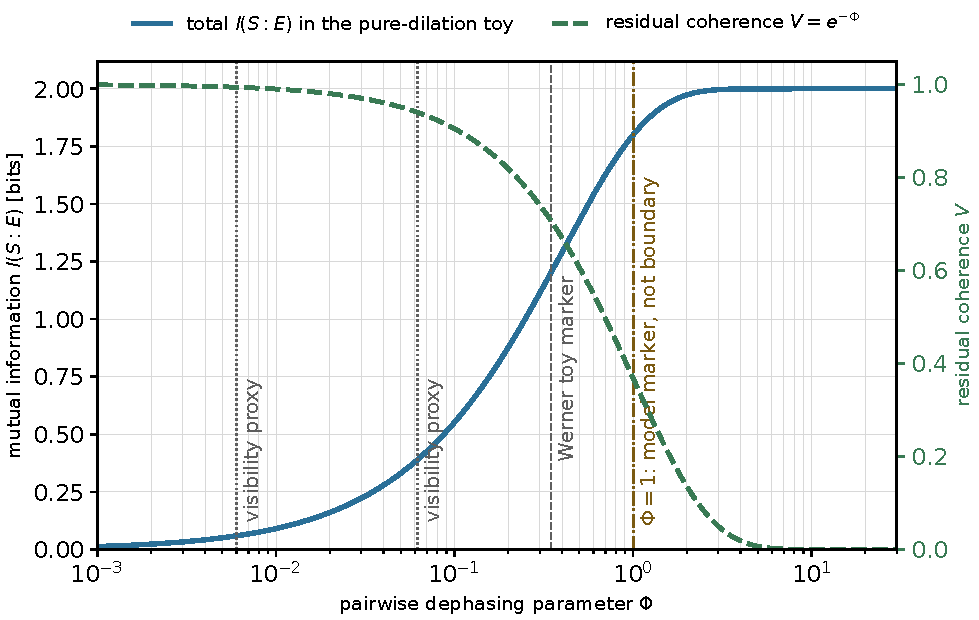
\includegraphics[width=0.90\textwidth]{../figures/r155/fig_qubit_info_decoherence_r155.pdf}
\caption{Declared pure-dilation qubit toy.  The mutual-information and
visibility curves are exact within that model.  The visibility and Werner
markers are source/model proxies, not ECT calibrations, collapse thresholds,
or metric-signature boundaries.  \textit{Display semantics: \detokenize{Both continuous traces are analytic relations of the declared pure-dilation toy; no sampled-data markers are implied.}}}
\label{fig:pop_qubit}
\end{figure}

Specified environmental channels can suppress interference and form stable
reduced-state records.  The physical record operator, environmental state,
and protocol determine the pairwise exponent; neither the total mode count nor
one universal dephasing scalar fixes the crossover.  Decoherence does
not select one ontologically realised outcome, and the pointer/update problem
remains Open.

Environmental decoherence is the standard reduced-state loss of visibility
caused by specified channels such as thermal photons, gas collisions or
phonons after their unresolved records are traced out.  This is a physical
open-system process, not an observer-induced projection postulate.

For gravity, the symbolic Di\'osi--Penrose formula remains an external
comparator, not an ECT-derived rate.  At fixed $\alpha,\beta$, about homogeneous $\bar n=w$, the projected tangent-director linear density vertex is missing; quadratic, nonlinear, composite and additional-field routes remain parametric/Open, the scalar trace vertex is only parametric, and the relevant ECT
state/noise kernel is Open/Not Identifiable.

\paragraph{DP-02 owner firewall.}
The tested candidate channels do not supply the physical ECT projector,
vertex, state-dependent noise kernel or reduction-rate map needed to identify
the external Di\'osi--Penrose infrared comparator.  No ECT coefficient or
collapse time follows; the state, pole, vertex and normalisation remain Open.

C$_{60}$ and macromolecular interference are standard environmental-
decoherence source-model anchors.  Quantitative visibility times must be
computed from the declared collision/radiation channel, state, coupling-rate
convention and observation protocol; no universal numerical object list is
published.

Partial recoherence is possible in specified echo or control protocols.
Reversing a declared reduced channel does not produce a universal backward
probability law: the reverse dynamics, preparation and path measure must be
defined separately.

\section{Quantum gravity in ECT}
\label{sec:pop_qg}

In standard approaches, quantum gravity --- the unification of GR and QM --- is one of the central unsolved problems of physics. Loop quantum gravity, string theory, causal dynamical triangulations, and other programmes attempt to quantise the gravitational field on a pre-existing spacetime or to construct spacetime from more fundamental elements.

ECT currently supplies quantum/open-system reconstruction routes and a scalar characteristic geometry inside one ordered-medium architecture.  It has not derived a physical graviton, universal gravity metric, common canonical action scale or gravitational record channel.  Quantum gravity is therefore an Open completion programme, not an already unified pair of derived sectors.

The scalar running and its Landau-pole estimate do not constitute graviton-loop power counting and do not prove improved ultraviolet gravity.  Newton's constant is only matched inside a supplied gravity completion; the bridge from condensate stiffness to its canonical tensor normalisation is Open.  Any UV advantage must be established from the constrained physical tensor propagator, vertices, counterterms and RP/OS reconstruction.

The open sequence begins earlier: derive a constrained physical tensor action, source, positive residues and canonical normalisation; only then attempt tensor-loop power counting, coupled RG and RP/OS reconstruction. OS reconstruction yields a Hilbert space only after the complete applicable corrected OS-II package---including correlators/measure, observable algebra and reflection, regularity/growth, covariance, RP, symmetry and applicable locality/cluster conditions---is proved; it does not create the missing physical tensor dynamics, clock or metric. These are open problems, not solved theorems (\emph{Level~Open}). Thus ECT reframes the question ``how do you put gravity and quantum mechanics together?'' through a single-medium architecture, while the full UV/spin-2 closure remains open.


\section{Reduced-state reformulation of the gravity--matter problem}
\label{sec:pop_hybrid_consistency}

A long-standing difficulty, often called the \emph{hybrid-consistency problem},
is that combining quantum matter with any non-quantised or emergent
description of gravity runs into a characteristic set of obstructions:
reduced states must remain positive; no classical channel should
transmit quantum information; energy--momentum bookkeeping must stay
controlled; relativistic compatibility and diffeomorphism invariance
must be preserved. Historical semi-classical proposals by M{\o}ller
and Rosenfeld already exhibited these tensions; later thought
experiments and effective-field-theory analyses sharpened them further.
Modern hybrid frameworks, such as post-quantum classical gravity
(PCCG), accept these tensions as part of a fundamentally stochastic
and irreversible law of gravity (\emph{Level~B for the general
landscape}).

ECT takes a candidate architectural route (Level~B/Open).  Information
preservation is a requirement on a future global interacting completion, not
an established postulate or theorem of P1--P6.  Reduced coherent
and classical-looking descriptions may arise after tracing specified channels;
however, a shared medium alone does not imply a nonfactorising physical state,
entanglement, or a gravity-mediated quantum channel.  Those require an explicit
state, vertex, kernel, and reduction map and remain Open.

\section{Gravity-induced entanglement: can gravity be ``classical''?}
\label{sec:pop_gie}

One of the sharpest near-term tests of the quantum character of
gravity is the proposal, due independently to Bose, Mazumdar and Morley
and to Marletto and Vedral~\cite{Bose_Mazumdar_Morley_2017,Marletto_Vedral_2017_GIE}, to look for entanglement between two
small mesoscopic masses held in spatial superposition and interacting
only through their mutual gravitational field. In its standard
reading, \emph{Gravity-Induced Entanglement} (GIE) in such a setup
would force the conclusion that the gravitational mediator itself
carries non-classical degrees of freedom, because local classical
channels cannot transmit quantum information. A refinement due to
Christodoulou and collaborators showed that the effect admits a
consistent locally mediated reading within linearised quantum
gravity, with proper causal retardation.

This standard inference has more recently been stress-tested.
A proposal by Aziz and Howl argued that, once matter is treated
at the level of quantum field theory, a locally classical-looking
gravitational coupling might still generate entanglement; several
critical responses argued that in the specific nonrelativistic
limit employed, the relevant unitary factorises and no genuine
gravity-mediated entanglement is produced. On the constructive side,
Trillo and Navascu\'es established that a Di\'osi--Penrose-type
classical gravity, treated as a \emph{correlated-noise} mechanism,
\emph{can} generate gravity-induced entanglement in that specific
model class. In other words, once one admits common-medium or
correlated-noise structure between the probe masses, the slogan
``classical gravity cannot entangle'' is no longer generally valid.

\textbf{Three disciplined claims about ECT.}
(\emph{A}) ECT does not take the observation of gravity-induced
entanglement in a mesoscopic protocol, by itself, to force a
fundamentally quantised independent metric field; once common-medium
loophole classes are admitted, the standard no-go inference applies
most directly to strictly local factorising classical channels.
(\emph{B}) ECT-specific gravity-induced entanglement is currently \texttt{NOT IDENTIFIABLE}; an external loophole class may allow it only if a derived reduced channel is shown to
arise whenever the experimentally relevant reduced dynamics still
retains common-medium non-factorisable structure --- that is, when
the protocol probes a Level~IIa regime rather than a Level~IIb
regime. (\emph{C}) ECT does not yet establish, from first principles,
which exact experimental protocols realise Level~IIa, nor does it
yet derive the explicit reduced mediator channel through which
entanglement would be generated (\emph{Level~Open}).

\textbf{Operational criterion.}
The architectural position of ECT in the BMV debate can be stated
sharply. ECT falls under the standard no-go logic only if, in the
actual regime realised by the experiment, the effective reduced
mediator is well approximated by a strictly local classical
factorising channel with no residual common-medium correlations.
ECT \emph{escapes} that logic if the experimentally relevant reduced
dynamics still retains correlated common-medium structure --- i.e.\
belongs to the Trillo--Navascu\'es loophole class. Different
protocols probe different reduced regimes of one underlying
condensate theory; ECT does not claim both descriptions for one and
the same operational regime.

\textbf{Imported benchmark formula and required apparatus inputs.}
Inverting the external unit-coefficient Di\'osi--Penrose scaling
$\tau_{\rm DP}^{\rm ext}\sim\hbar R/(G_Nm^2)$ at a supplied fixed radius and
declared coherence time defines the guide
\[
 m_{\rm guide}^{\rm DP}
 \sim \sqrt{\hbar R/(G_N\tau_{\rm exp})}.
\]
It is not an environmental crossover and is not a scalar-sector or
entangling-channel ECT prediction.  If one separately supplies the hard-sphere
collisional rate $\lambda_{\rm coll}=n_{\rm gas}v_{\rm th}\pi R^2$ for a
homogeneous sphere $m=4\pi\rho R^3/3$, and the unit-coefficient external rate
$\lambda_{\rm DP}^{\rm ext}=G_Nm^2/(\hbar R)$, equality gives
\[
 R_{\rm cross}^{\rm coll-DP}
 \sim\left(\frac{9\hbar n_{\rm gas}v_{\rm th}}
 {16\pi G_N\rho^2}\right)^{1/3},
 \qquad
 m_{\rm cross}^{\rm coll-DP}
 \sim\frac{3\hbar n_{\rm gas}v_{\rm th}}{4G_N\rho}.
\]
This is exact algebra inside the two displayed approximate source models, not
a universal collapse law or an ECT crossover.  It deliberately uses a unit
coefficient.  A separate external continuum-sphere orientation fixes the
factor-$1/2$ functional and explicitly adopts $\tau=\hbar/E_G$ for two identical sharp
homogeneous spheres, centre-to-centre separation $d=R$, and
\[ R=1\,\mu\mathrm m,\qquad \rho=2000\,\mathrm{kg\,m^{-3}}. \]
For that nominal point only,
\[
 C_{\rm DP}(1)=\frac{51}{160},\qquad
 \tau_{\rm DP}^{\rm ext}=70.6\,\mathrm{ms}.
\]
This is Level-A geometry inside an imported source model and an external
Level-C benchmark; it is not a data test, physical uncertainty statement or
ECT collapse time.  Profiles, smearing, separation, regularisation and
normalisation change it.  Inserting $51/160$ into the unit-coefficient guide
or crossover would change their coefficients and therefore would define a
different comparator.

A physical apparatus comparison requires the gas species and equation of
state, $P$ and $T$, a thermal-speed convention, total or differential cross
section, target and chamber geometry, spatial-superposition profile, and the
coherence-time/visibility protocol.  A completed ECT calculation would
additionally require the physical projector, vertex, state-dependent noise
kernel, finite-body charge and absolute normalisation, all presently
Open/Not Identifiable.


\section{How gravity may talk to matter: candidate record channels}
\label{sec:pop_mediator}

The following split is an operational taxonomy, not a derivation of two
physical ECT baths.

\textbf{Scalar trace-response candidate.}
The scalar-only action yields a parametric canonical coupling to the matter
trace $T$.  It does not by itself determine a state-dependent noise kernel,
a finite-body charge, or an absolute decoherence rate.  The fixed-radius unit-coefficient
$m_{\rm guide}^{\rm DP}\sim\sqrt{\hbar R/(G_N\tau_{\rm exp})}$ is therefore
only a benchmark relation after the required apparatus inputs and coherence
protocol are supplied; it must not be confused with
$m_{\rm cross}^{\rm coll-DP}$, which additionally depends on the supplied gas
and density model, or with the separate geometry-resolved
$C_{\rm DP}(1)=51/160$, $70.6\,\mathrm{ms}$ sphere point.  None is an
ECT-derived rate.

\textbf{Orientation/tensor candidate.}
An orientation channel could in principle provide a common retarded mediator,
but the displayed scalar action contains no $n^A$ sector and does not derive
its matter-density projector.  A covariant orientation action, its metric and
matter vertices, the physical state, and the Hadamard/noise kernel are all
required before this candidate can be classified quantitatively.

\textbf{Status.}
Response, noise, and entangling capacity must be kept distinct.  Reusing a
static gravitational response as a stochastic noise kernel would double-count
the same physics unless a subtraction is specified.  The ECT gravitational
record channel is therefore Open/Not Identifiable.  The Di\'osi--Penrose functional, the declared geometry-resolved
sphere point, fixed-radius unit-coefficient $m_{\rm guide}^{\rm DP}$ relation
and conditional unit-coefficient collisional
$m_{\rm cross}^{\rm coll-DP}$ comparison are distinct external comparators;
no numerical D--P/environment crossover or ECT rate is published.

\begin{figure}[p]
\centering
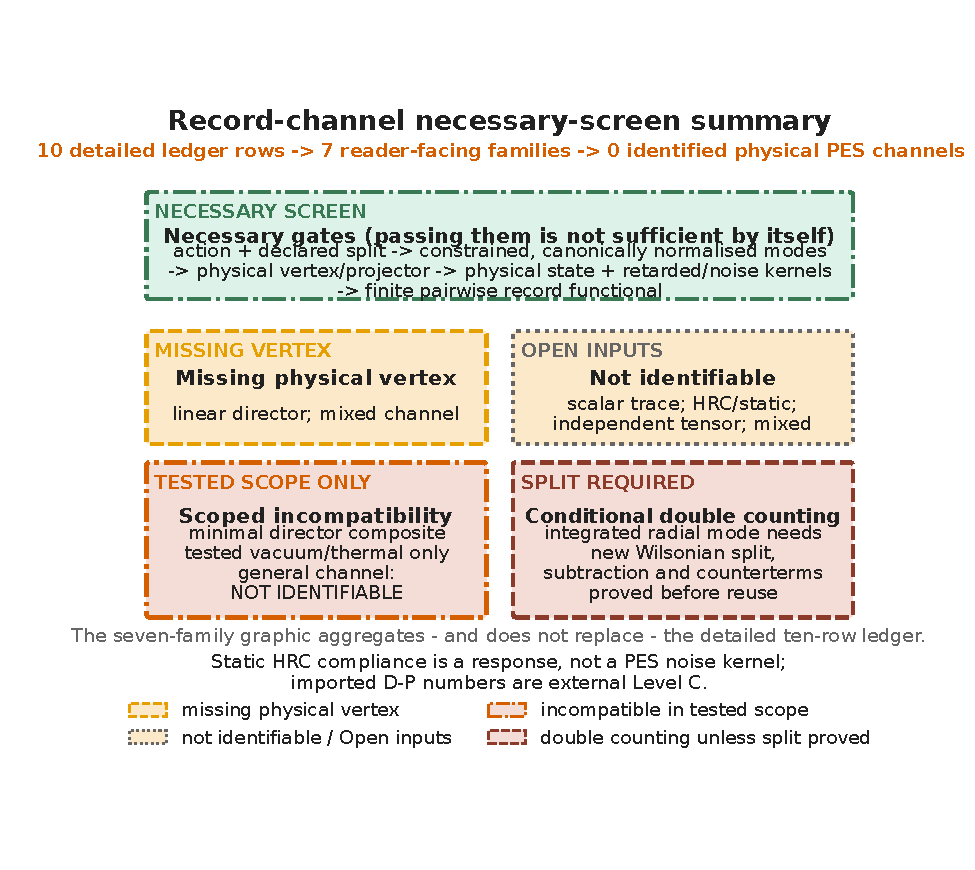
\includegraphics[width=\textwidth]{../figures/r149/r149_mediator_channels_summary_47C.pdf}
\caption{Reader-facing necessary-screen summary of the bounded record-channel audit.
The graphic aggregates, but does not replace, the authoritative ten-row
candidate/subcase ledger.  No tested row supplies the complete action-owned
physical modes, vertex/projector, state, retarded/noise kernels and finite
pairwise record functional.  The general channel remains
\texttt{NOT IDENTIFIABLE}; reuse of an integrated radial mode is
\texttt{DOUBLE-COUNTED} unless a new Wilsonian split and subtraction ledger
are proved; the Di\'{o}si--Penrose functional remains an external comparator.
Passing this screen would be necessary, not sufficient, for a physical PES
channel.  The complete connected Part~III A4 reader map and its deterministic
exact-key and machine-topology records preserve the canonical source labels,
edge inventory and status provenance without duplicating them here.}
\label{fig:pop_mediator_channels}
\end{figure}

\section{The infrared sky: asymptotic symmetries, memory, and soft gravitons}
\label{sec:pop_ir_soft}

Modern general relativity has sharpened an old intuition: at very
long wavelengths, near null infinity, there lives a rich structure of
\emph{asymptotic symmetries}, \emph{gravitational memory}, and
\emph{soft gravitons} that goes far beyond the naive
Minkowski-at-infinity picture. The asymptotic symmetry group
discovered by Bondi, van der Burg, Metzner, and Sachs (BMS) is an
infinite-dimensional extension of Poincar\'e symmetry; gravitational
memory is the permanent shift left behind in the metric at null
infinity after a burst of gravitational radiation passes; soft
graviton theorems connect zero-energy gravitons to both BMS
supertranslations and memory through the modern ``asymptotic symmetry
/ soft theorem / memory'' triangle.

ECT offers a candidate infrared interpretation (Level~B/C
compatibility only) in asymptotically flat ordered-branch settings.  The
asymptotic data $(\phi_0,n_A^{(0)})$ provide a possible stage for a BMS
analysis, and a persistent $\Delta n_A$ shift is a candidate memory variable.
However, the covariant orientation action, its TT spin-2 mode, asymptotic
charges, soft theorem, and memory map have not been derived.  Long-wavelength
$\delta n_A$ modes therefore cannot yet be called physical ECT soft gravitons,
and no first-principles BMS/memory/soft triangle is claimed.

\textbf{Caveat.}
The existence of soft modes does not, by itself, solve any
information problem; it only identifies a potentially relevant
low-energy bookkeeping sector. Whether the long-wavelength
$\delta n_A$ modes suffice to store and recover the information
content required by black-hole evaporation is not established here
and is not claimed.


\section{Black-hole thermodynamics and the information problem}

ECT investigates a C/Open completion in which the black-hole horizon is
represented by a condensate interface.  The current action does not derive
that interface, Hawking emission, or controlled corrections; this section
separates generic reduced-state mathematics from the supplied shell toy.

\begin{figure}[tbp]
\centering
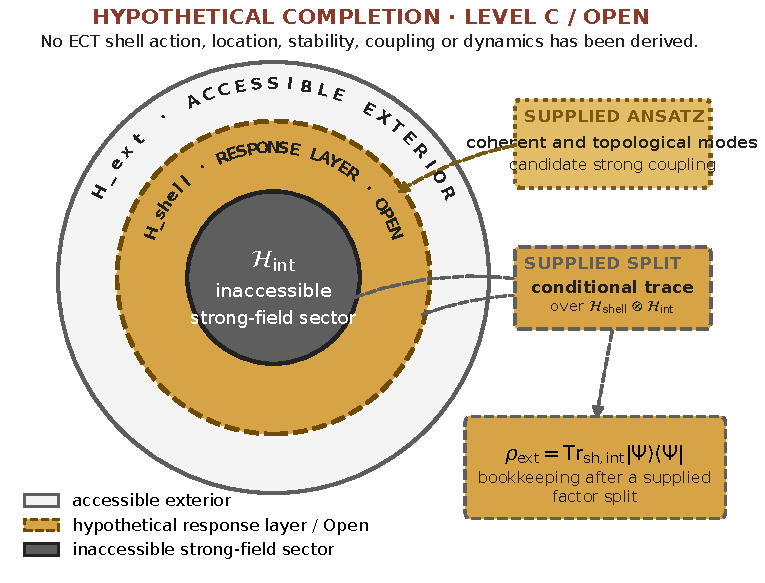
\includegraphics[width=0.84\textwidth]{../figures/r155/fig_bh_shell_r155.pdf}
\caption{Candidate Level-C/Open critical-shell picture.  The amber callout is
the supplied strong-coupling ansatz for coherent and topological modes.  Two
gray leader lines select shell and interior factors for a conditional trace;
they are not dynamical arrows.  The sole gray arrow runs from the trace
operation to the reduced exterior state.  The factor split, shell
geometry, correlations and Euclidean-core continuation remain Open.
Reduced-state thermality is compatible with global purity, but P1--P6 do not
yet prove globally unitary interacting strong-field evolution or
outgoing-correlation recovery.}
\label{fig:pop_bh}
\end{figure}

If information falls into a black hole and the black hole evaporates via Hawking radiation, is the information lost? This is the information paradox --- one of the deepest problems in theoretical physics.

\paragraph{Premise and ownership audit.}
The information problem arises from the simultaneous use of semiclassical
effective field theory, quantum unitarity, a regular horizon, evaporation and
an inside/outside factorisation (together with the applicable locality and
causal assumptions).  Merely declaring Lorentzian geometry or the horizon
``emergent'' does not identify which premise fails and does not solve the
problem.  ECT has not yet derived the physical shell, metric, subsystem
factorisation or evaporation channel.  Conditional on supplying them,
Hawking-like thermality may be represented as reduced-state thermality,
\[
  \rho_{\rm ext}
  =
  \mathrm{Tr}_{\rm shell,int}\,
  |\Psi\rangle\langle\Psi|,
\]
not by itself evidence for destruction of a full condensate state. The question ``is information lost?'' therefore splits into two questions.  The general reduced-state identity is exact; whether ECT possesses a globally unitary interacting strong-field completion, and whether outgoing radiation recovers the correlations, remain separate Open questions.

ECT addresses it at two levels (Fig.~\ref{fig:pop_bh}).

\textbf{Conditional global-unitarity hypothesis:} If a completed ECT strong-field theory supplies a global Hilbert space, physical subsystem split and isometric interacting evolution, then $\rho_{\rm ext}={\rm Tr}_{\rm shell,int}|\Psi\rangle\langle\Psi|$ can be mixed while the global state stays pure.  This excludes only a complete state-erasing final channel; one-body thermal spectra can remain exact with information in phases or higher correlations.  P2 does not construct the Hilbert space, Hamiltonian, factorisation, evaporation channel or Page curve.

\textbf{Level~C/Open (shell ansatz and optional $H_{\rm sh}$ completion):}
A candidate critical shell is supplied as a possible transition between
effective regimes.  The named optional stationary passive-scattering
completion $H_{\rm sh}$ uses natural units $\hbar=c=1$, a dimensionless shell
field $[\chi_{\rm sh}]=1$, and local coefficients
$a_{\rm sh}>0$, $\lambda_{\rm GL}>0$, with
$[a_{\rm sh}]=E^2$ and $[\lambda_{\rm GL}]=E^4$.  The symbols
$a_{\rm sh}$ and $\lambda_{\rm GL}$ belong only to this shell closure and are
not the P3 gradient or quartic coefficients.  The completion also supplies an
independent self-adjoint
Sturm--Liouville problem on $I_\rho\subset(\rho_c,\infty)$ with positive
coefficient and weight.  A declared flux-normalised channel may be written
$\mathcal T_{\omega\ell}[\bar\chi_{\rm sh}]
=\exp(i\delta_{\omega\ell}-\Gamma_{\omega\ell})$, with
$\delta_{\omega\ell}\in\mathbb R$, $\Gamma_{\omega\ell}\ge0$ and
$0<|\mathcal T_{\omega\ell}|<\infty$; passivity gives
$|\mathcal T_{\omega\ell}|\le1$ only in that flux convention.  After fixing a
logarithm branch and radial mode projection, its supplied Fr\'echet kernel is
$K_{\omega\ell}(\rho):=\left.\delta\ln\mathcal T_{\omega\ell}[\chi]
/\delta\chi(\rho)\right|_{\bar\chi_{\rm sh}}$, with
$\delta\ln\mathcal T_{\omega\ell}=\int_{I_\rho}d\rho\,
K_{\omega\ell}(\rho)\delta\chi_{\rm sh}(\rho)$ and
$[K_{\omega\ell}]=E$.  One supplied local vertex may be
$\mathcal L_{\rm int}^{H_{\rm sh}}=-g\,\delta\chi_{\rm sh}
(\partial\varphi)^2/2$, where a canonically normalised four-dimensional probe
has $[\varphi]=E$ and the independent coefficient $g$ is dimensionless and may
vanish.  The background, state, Hamiltonian coefficients, Green function,
interval, boundary data, flux normalisation, kernel and detector map are
completion inputs; mode mixing, resonances, superradiance or nonstationarity
require another representation.  Neither this closure nor the area-cell and
finite-memory toys derive a physical shell, Hawking spectrum, entropy
coefficient, evaporation channel, Page curve, echo, ringdown or interior
geometry.



\textbf{Three-regime structure.}
The supplied thermal-shell toy labels three candidate regimes:
(i)~an exterior region where standard effective geometry is assumed;
(ii)~a candidate shell/interface regime, where a toy ordered-branch amplitude is assumed to change;
and (iii)~a proposed non-geometric core.  No physical crossover temperature, metric breakdown or universal shell thickness is derived; the Tolman toy contains only $\rho_*=\hbar c/(2\pi k_BT_*)$.

\textbf{Topological consistency.}
The identity $\pi_2(S^3)=0$ says only that a supplied $S^2$ shell map need not carry $\pi_2$ charge; it does not derive formation, dissolution, stability, or dynamics of a shell.
The nontrivial sector $\pi_3(S^3) = \mathbb{Z}$ admits possible topological configurations, but the present work does not derive a stabilising Skyrme-type term or a finite-energy gravitating topological black-hole solution.

\textbf{What is not yet derived.}
The present shell analysis does not yet derive the full interior profile, first-principles horizon thermodynamic coefficients, or a constructive Page curve.

\textbf{Comparison with the islands / quantum-extremal-surface language.}
The modern holographic programme approaches the same black-hole
information question through a different language: the \emph{islands
formula} and the notion of \emph{quantum extremal surfaces} (QES).
In that language, the entropy of Hawking radiation is computed as a
generalised entropy
$\mathrm{Area}(\partial\Sigma)/(4\,G_N)+S_{\rm bulk}(\Sigma)$, with the
applicable extremisation and minimisation prescription.  In representative
semiclassical evaporating-black-hole models, the trivial saddle dominates
before the Page time, while a nontrivial island saddle can dominate after it
and produce a Page-curve turnover.
The candidate shell and islands/QES pictures admit a C/Open analogy
only after global unitarity and physical subsystem algebras are
supplied.  ECT derives neither a shell/interior factor nor a QES, so no
physical equality of roles is asserted.
Crucially, the critical-shell boundary is \emph{not} identified here
with a derived quantum extremal surface, and ECT does not derive
the generalised-entropy formula or carry out a replica-wormhole-type
calculation on its underlying Euclidean condensate path integral;
those remain open tasks. The point of the mapping is compatibility
of structural logic, not an ECT derivation of the Page curve.

\section{Area-law entropy: a conditional medium programme, not yet an ECT theorem}
\label{sec:pop_area_law}

Black-hole entropy and gravitational entropy-bound arguments motivate area
scaling in specified gravitational regimes; they do not imply a universal
area law for arbitrary regions or states.  Bekenstein's black-hole and
entropy-bound work, and the later holographic proposals of 't~Hooft and
Susskind, have shaped much of modern theoretical physics.
In string theory it appears as the AdS/CFT duality; in loop quantum
gravity it emerges from a counting of quantum-geometric states.
In both cases, however, area scaling is tied to specific features of
the gravitational theory.

ECT offers a possible medium interpretation, but an important
distinction is essential.  The radial mass $m_\sigma$ sets a
correlation length and the breakdown scale of a reduced EFT.  It does
\emph{not} by itself provide a microscopic lattice spacing, a hard UV
cutoff, or a finite-dimensional cell.  A massive continuum field still
has arbitrarily short-wavelength modes, and its entanglement entropy is
UV divergent.

Nor does locality plus a finite two-point correlation length prove an
area law for every state: volume-law and data-hiding states are not
excluded by those facts.  The honest surviving result is therefore a
conditional counting lemma.

\paragraph{Conditional boundary-cell count.}
Draw a closed surface~$\Sigma$ only after a physical subsystem split
has been supplied.  Also supply (i)~a coarse-graining or microscopic
resolution $\ell_{\rm cg}$, (ii)~a finite entropy capacity
$s_{\rm cg}$ per retained cell under a stated truncation or energy
restriction, and (iii)~a state class whose cross-interface entropy is
localised, up to $\Delta S$, in a layer of thickness $\xi_{\rm ent}$.
The last input may follow from a separately proved finite-depth,
Markov, or area-law property; it does not follow from finite correlation
length alone.  Counting cells then gives
\begin{equation}
  S_{\rm red}(\Sigma)
  \;\le\;
  C_\Sigma s_{\rm cg}
  \frac{A(\Sigma)\xi_{\rm ent}}{\ell_{\rm cg}^{3}}
  +\Delta S.
\end{equation}
Only with the additional matching
$\xi_{\rm ent}=O(\ell_{\rm cg})$ and sub-area $\Delta S$ does this
reduce to $S_{\rm red}=O(A/\ell_{\rm cg}^2)$.  The implication is
Level~A mathematics under its supplied assumptions; ownership of those
assumptions by ECT is Open.

\paragraph{Why this is not just a restatement of the QFT result.}
In local quantum field theory, the leading ultraviolet-sensitive term in the
vacuum entanglement entropy of many low-energy states often obeys an area law.
Its coefficient is regulator- and renormalisation-scheme dependent.  This
standard result does not by itself supply a physical ECT cutoff or entropy
coefficient.

The present continuum ECT action does not upgrade or remove that
divergence.  Identifying its regulator with $m_\sigma^{-1}$ would
confuse an EFT breakdown/correlation scale with a UV completion.

\paragraph{Black-hole entropy as a special case.}
The shell-entropy result discussed earlier,
$S_{\rm shell}^{\rm toy}\sim A\ln q/\ell_{\rm cg}^2$,
is one instance of the conditional count only after a physical shell,
factorisation, cell scale, finite local dimension~$q$, and suitable
state have all been supplied.
The exact Bekenstein--Hawking coefficient $1/(4\ell_{\rm Pl}^2)$
is merely a target matching condition inside that toy; it does not
derive a black-hole capacity or the microscopic scale.

\paragraph{Strengthening the Page-curve programme.}
The general area bound has an important consequence for the
information paradox.
The boundary-layer bound does not derive a physical shell, its Hilbert
capacity, or an evaporation channel.  Accordingly it neither proves a
finite information reservoir nor strengthens the conditional isometry
identity.  Thermal marginals and the Page-curve shape remain unfixed.
A complete Page-curve derivation still requires additional
dynamical ingredients (information return mechanism, purification
dynamics), which remain open.

\paragraph{Connection to decoherence.}
An interface may also enter a supplied open-system model, but the
cell-counting lemma gives no decoherence kernel, no entropy-production
theorem, and no PES result.

\paragraph{From area law to holography.}
It is important not to overclaim.
ECT currently establishes only the conditional finite-cell implication.
It does not yet establish:
\begin{itemize}[nosep]
  \item a physical ECT area law for the completed state;
  \item a covariant entropy bound analogous to the Bousso bound
    for dynamical horizons;
  \item a full bulk-boundary reconstruction (a gravity/boundary
    duality of the AdS/CFT type);
  \item a complete holographic principle in the strongest
    reconstruction sense.
\end{itemize}
The correct summary is:

\emph{ECT provides an interface-motivated programme and an explicit
list of missing microscopic/state inputs.  A physical area law and
full holography remain Open.}

\paragraph{How ECT differs from other approaches.}
In AdS/CFT, area scaling arises from a duality between a
gravitational theory in the bulk and a conformal field theory on
its boundary.
In loop quantum gravity, it arises from counting discrete
quantum-geometric states.
In ECT, a boundary-cell picture is a candidate only.  It becomes an
alternative physical explanation if a microscopic completion derives
the split, finite local capacity and area-law state class instead of
assuming them.

\paragraph{What remains open.}
The microscopic resolution and local capacity, the physical subsystem
split, the relevant state theorem, soft/gauge-edge sectors, the
black-hole shell and coefficient, and any covariant null-surface bound
all remain Open.


\section{What the compact phase does---and does not---establish about charge}
\label{sec:pop_charge}

The coherent branch contains a compact coordinate,
\[
\theta \sim \theta + 2\pi.
\]
This proves the existence of integer \emph{winding sectors} of that
coordinate.  It does not by itself prove that the coordinate is the
physical electromagnetic gauge fibre, that its redundant directions
have been quotiented correctly, or that an unbroken massless connection
couples to matter.

There is a useful conditional theorem.  If a completed ECT sector
provides a compact physical $U(1)$ principal bundle, a gauge-reduced
kinetic operator, and matter representations of that group, then the
representation weights are integer relative to a chosen elementary
normalisation:
\[
q = n\,e_0, \qquad n\in\mathbb{Z}.
\]
Likewise, the compact generator has a discrete spectrum only after a
physical Weyl representation, its action normalisation and a
self-adjoint quasiperiodic domain have been supplied.  For twist
$\nu_{\rm tw}$ the spectrum is
$S_0(\mathbb Z+\nu_{\rm tw}/2\pi)$; the lattice $S_0\mathbb Z$ is
only the periodic special case.  This generator is not thereby the
electric-charge operator, and compact field winding is a separate
topological integer.  These are standard consequences \emph{inside} a
completed compact-$U(1)$ representation; ECT has not yet derived the
physical charge map (\emph{B/Open}).  A charged condensate can also
Higgs the candidate connection, so an unbroken photon must be shown
rather than assumed.

\paragraph{Open physical owners.}
ECT must still derive the gauge volume or reduced Hessian, Maxwell
normalisation, the identity of $U(1)_{\rm em}$, its unbroken photon,
the charge operator, and the matter map.  The observed Standard-Model
pattern additionally requires electroweak embedding,
\[
Q = T_3 + \frac{Y}{2},
\]
the colour sector, anomaly-consistent matter representations, and the
global gauge-group quotient.  The recorded colour-interlock layer is a
consistency condition on completions: with the
standard $\mathbb{Z}_6$-type global quotient, hypercharge, colour
and weak data must satisfy an explicit congruence, which fixes the
fractional electric pattern per colour class
($Q \equiv -t/3 \pmod 1$) and reduces the residual freedom to an
explicitly characterised discrete family. This is a consistency
requirement on completions, not a derivation of the observed
hypercharges.

\section{Why the post-Big-Bang Universe developed the way it did}
\label{sec:pop_post_transition}

ECT offers a candidate Level~B/Open branch-boundary interpretation of one
part of the Big-Bang question: a P1 Euclidean configuration class and a
separately supplied P4 ordered class may be related by ordering dynamics.
Calling that relation the physical Big-Bang boundary requires a state,
clock/lapse, observable metric and transfer to matter and radiation; it is
not a chronology theorem of P1--P6.

But this still leaves a second question: once the ordered branch
has formed, why does the Universe then evolve in the way we observe?

ECT does not yet solve the full transition dynamics.
In the main preprint this open problem is now decomposed into four
parts of very different difficulty: the ordering mechanism itself,
the orientation of the branch (why expansion), the thermal completion
into a hot Big-Bang history, and the observable relics of the
ordering event.
The orientation question has recently been sharpened in two steps.
First, the homogeneous background equations turn out to be blind to
the sign of expansion on their own: until a thermodynamic arrow of
time is fixed, an ``expanding'' and a ``contracting'' description are
two parametrisations rather than two physically distinct options, so
part of the old question dissolves.
Second, once the arrow of time is fixed, a conditional no-bounce
result applies in the spatially flat positive-potential/no-ghost sector: a
smooth solution cannot change the sign of $H$.  This does not determine the
sign of $\dot H$, monotonic growth of density or curvature, or a breakdown
timescale.  Contracting de~Sitter supplies an explicit counterexample to that
stronger inference.  A separately conserved component with $w>-1$ does grow
on a contracting branch, but promoting this to total breakdown requires a
complete action, state, energy-exchange law and threshold.  The physical
branch orientation, ordering mechanism and thermal completion therefore
remain Open rather than being selected by persistence alone.

Within the explicitly supplied scalar actions one can classify
conditional post-transition histories.  The two-slope completion provides a
regular radiation--matter--de-Sitter proof of class.  Separately, its bare
positive-kinetic scalar pieces obey $w_\phi^{\rm bare}\ge-1$ when
$K_\phi^{\rm phys}+U>0$; non-minimal $F,\dot F,\ddot F$ terms leave the
observable $w_{\rm eff}$ unconstrained.  These are action-internal statements:
they do not show that the physical ECT condensate follows that history,
preserves standard early cosmology, or owns the observed late acceleration.

In condensed-matter systems, ordered domains often grow into a disordered
environment.  Applying that picture to ECT is only a conditional analogy:
the present action does not derive the relevant nonequilibrium front, its
clock, or the selection of an expanding physical branch over a contracting
one.

Other branches require their own complete action and state.  A contracting
branch is a kinematically admissible acceptance case; the growth analogy is
not evidence sufficient to disfavour it.  The named positive-potential
two-slope action tends to its stable de-Sitter root and does not produce
recollapse.  A contracting or recollapsing branch remains an Open acceptance
case for a different explicitly supplied action/state; no ECT recollapse
timescale has been derived.  The inequality
$w_\phi^{\rm bare}\ge-1$ excludes only a phantom \emph{bare ratio} inside the
supplied positive-kinetic decomposition when
$K_\phi^{\rm phys}+U>0$; it does not exclude an observable
$w_{\rm eff}<-1$ history generated by non-minimal terms.

The theory therefore supplies a programme for comparing ordered-branch
cosmologies once an action, state and clock/metric completion are specified.
It does not yet select the observed expansion history or derive a geometric
origin of the Big-Bang branch, and its hot radiation history remains Open.

\section{The grandfather paradox}

ECT does not yet solve the grandfather paradox; it provides a conceptual
programme for asking how causal worldlines could arise from a Euclidean
boundary-value ontology.

Classical causal paradoxes of time travel arise from trying to maintain two incompatible assumptions: that one can move backward along the physical time axis, and that causal chains remain linearly irreversible. The contradiction appears because the traveller is imagined as re-entering an already fixed causal sequence from within that sequence.

The coordinate $w$ is not a fundamental causal axis.  However, P1--P6 do
not yet derive a physical worldline map, a clock, controllable motion in
$w$, or a rule connecting global Euclidean configurations to observable
causal histories.  Therefore statements about a traveller moving backward
in $w$ or crossing an earlier worldline are not current consequences of
ECT.  The defensible claim is narrower: ordinary Lorentzian paradoxes need
not be primitive at the Euclidean level, while any physical resolution must
be demonstrated in a completed clock/metric/matter theory with operational
no-signalling and consistency tests.


\section{Analogue laboratory programme}

Superfluids, Bose--Einstein condensates, and related platforms are analogue systems for selected mechanism classes and conditional closures. They do not instantiate the full ECT vacuum: success is not evidence for ECT, and failure rejects only the explicitly mapped analogue implementation. Useful platforms include:

Superfluid $^4$He and Bose--Einstein condensates: phase-winding quantisation, vortex dynamics, Goldstone spectrum, and the condensate-mediated correlation structure.

Acoustic black holes (``dumb holes'') in BECs: analogue Hawking effect and critical-shell structure.

Boundary-response experiments can be specified only after a physical reduced ECT bundle, material boundary operator and stress response are derived.  At present no condensate-sector Casimir force is predicted.

Atom and mesoscopic interferometry: constraints on standard Di\'osi--Penrose benchmarks and on any future spectrally specified ECT record kernel.


\section{Conclusions of Part~III}

\subsection{Status-separated outcomes and Open owners}

The coherent-branch discussion contains the following conditional
mathematics, external targets, structural routes, and Open owner problems:

\begin{enumerate}
\item Conditional Hilbert-space route only through the complete applicable corrected OS-II package in the declared Gaussian/free kernels (A-math for those kernels); the interacting ECT measure, observable algebra, continuation/generator, clock/metric and canonical completion remain B/Open.
\item A supplied local KG-form scalar equation and a separately supplied Schr\"odinger-type complex law; their leading NR envelope relation is conditional A-level asymptotic mathematics only with the stated clock, mass, stable-frequency, weak-interaction, slow-envelope and residual-control inputs, while a common ECT descent and physical owner remain B/Open.
\item Linear superposition is A only in the verified quadratic subsector and B/Open physically; interference is B/Open; Pauli is A-math for the free antisymmetric kernel and B/Open for physical ECT matter.
\item Integer compact-phase winding sectors exist at Level~A; action normalisation and physical spectrum reconstruction are B/Open.
\item Compact-phase winding sectors (A) and a conditional Abelian connection/charge-lattice route (B/Open); physical $U(1)_{\rm em}$, photon, charge operator and matter map remain Open.
\item PES-R is a status-separated inventory of stationarity, record, finite-time, and protocol diagnostics (B); no universal selection theorem.
\item Conditional probability-representation route: a complete corrected OS-II package supplies a Hilbert space in verified subsectors; ordinary projector Gleason is Level-A mathematics only for complex dimension at least three with a supplied normalized, noncontextual, countably additive measure, while a qubit needs a separately supplied Busch effect/POVM or composite extension.  Dephasing is separate, and the physical ECT probability/Born owner remains Open.
\item Reduced-state dephasing only inside specified source models with declared coupling, state, kernel, trace and timescale (B/Open); the physical ECT channel, probability measure, pointer records, outcome and update remain Open.
\item Common-medium nonfactorisation as a candidate entanglement route (B/Open); Bell, no-signalling, and Tsirelson correlators remain Open.
\item Euclidean/WKB tunnelling as interpretive compatibility (B); no distinct ECT tunnelling derivation is claimed.
\item Supplied scalar Dirichlet BVP (A mathematics/Open ECT); no physical Casimir coefficient is predicted.
\item Standard Euclidean--Rindler/Unruh target (A external/Open ECT); physical state, cone, detector response and rate Open.
\item The external Di\'osi--Penrose functional and one scoped $51/160$, $70.6\,\mathrm{ms}$ sharp-sphere orientation point are retained; neither supplies an ECT coefficient or collapse time, and the ECT gravitational record channel remains Open/Not Identifiable.
\item Thermal marginals are compatible with global purity under a supplied split/isometry; global ECT black-hole unitarity is Open.
\item Bekenstein--Hawking area law as an external target; ECT coefficient and physical state owner Open.
\item Conditional boundary-cell counting lemma (A mathematics under supplied coarse-graining/state inputs; Open ECT).
\item Illustrative Page-curve-like turnover in a finite-memory shell toy model (\emph{C/Open}); a constructive ECT Page curve remains Open.
\item Quantum gravity structurally reframed by the single-condensate architecture; full UV and spin-2 closure remain open (\emph{B/Open}).
\end{enumerate}

\subsection{Key equations and principles of Part~III}

Winding condition: $\oint \partial_A\theta\,dX^A = 2\pi n$.

Loop-scale candidates: $\iota_{\rm elem}^{\rm(fixed\ core)}=2\pi \iota_0^{\rm EFT}$ in the phase-only model, which has no nonzero global minimum as $L$ varies; a BR1 phase-tension reduction may define $\iota_{0,\rm bal}^{\rm eff}$; and the separate texture-worldline modulus route defines $\iota_{0,\rm bal}^{(\vartheta)}$ only after its owner and proper-time ensemble are supplied.  CDE-$\Phi$ is an acceptance criterion rather than that owner.  The calibration $S_0=\hbar$ is Level~B; profile/Hessian, bending/barrier, stability, microscopic ownership and universality remain Open.

PES-R inventory: stationarity, pairwise record stability, and compact-phase admissibility are separate filters; a universal intersection theorem remains Open.

Source-model visibility proxy: $\tau_{\rm vis}=1/(N_{\rm eff}\gamma)$ only
after the channel, state, rate convention and observation protocol are
specified; it is not a universal ECT decoherence time or sector boundary.

Casimir: supplied $N$-scalar Dirichlet algebra only; for separately supplied $N=3$ the $3/2$ toy identity is retained, while the physical ECT bundle, boundary map, stress and force coefficient remain Open and no ECT correction is predicted.

BH entropy target: $S_{\rm BH}=A/(4\ell_{\rm Pl}^2)$; the current ECT shell toy derives neither this scaling nor its coefficient.

Conditional cell count:
$S_{\rm red}\le C_\Sigma s_{\rm cg}A\xi_{\rm ent}/\ell_{\rm cg}^3+\Delta S$;
an $A/\ell_{\rm cg}^2$ form needs separately supplied
$\xi_{\rm ent}=O(\ell_{\rm cg})$ and a sub-area remainder.

\subsection{Part~III status and dependency logic}

\begin{figure}[H]
\caption{Complete connected Part~III status and dependency map.  The single
colour-coded A4 reader map retains every canonical node and directed edge; node
text and adjacent prose carry the scientific qualifications, while arrows
organise declared dependencies and never upgrade status.  The deterministic
exact-key and machine-topology records preserve the canonical source labels
and edge inventory.}
\label{fig:pop_partIII_logic}
\end{figure}

Figure~\ref{fig:pop_partIII_logic} is kept as one connected graph, avoiding
the false impression that its quantum, PES-R, probability and application
branches are independent derivations.  The PDF remains vector content for
zooming and its literal status text is authoritative.

\clearpage
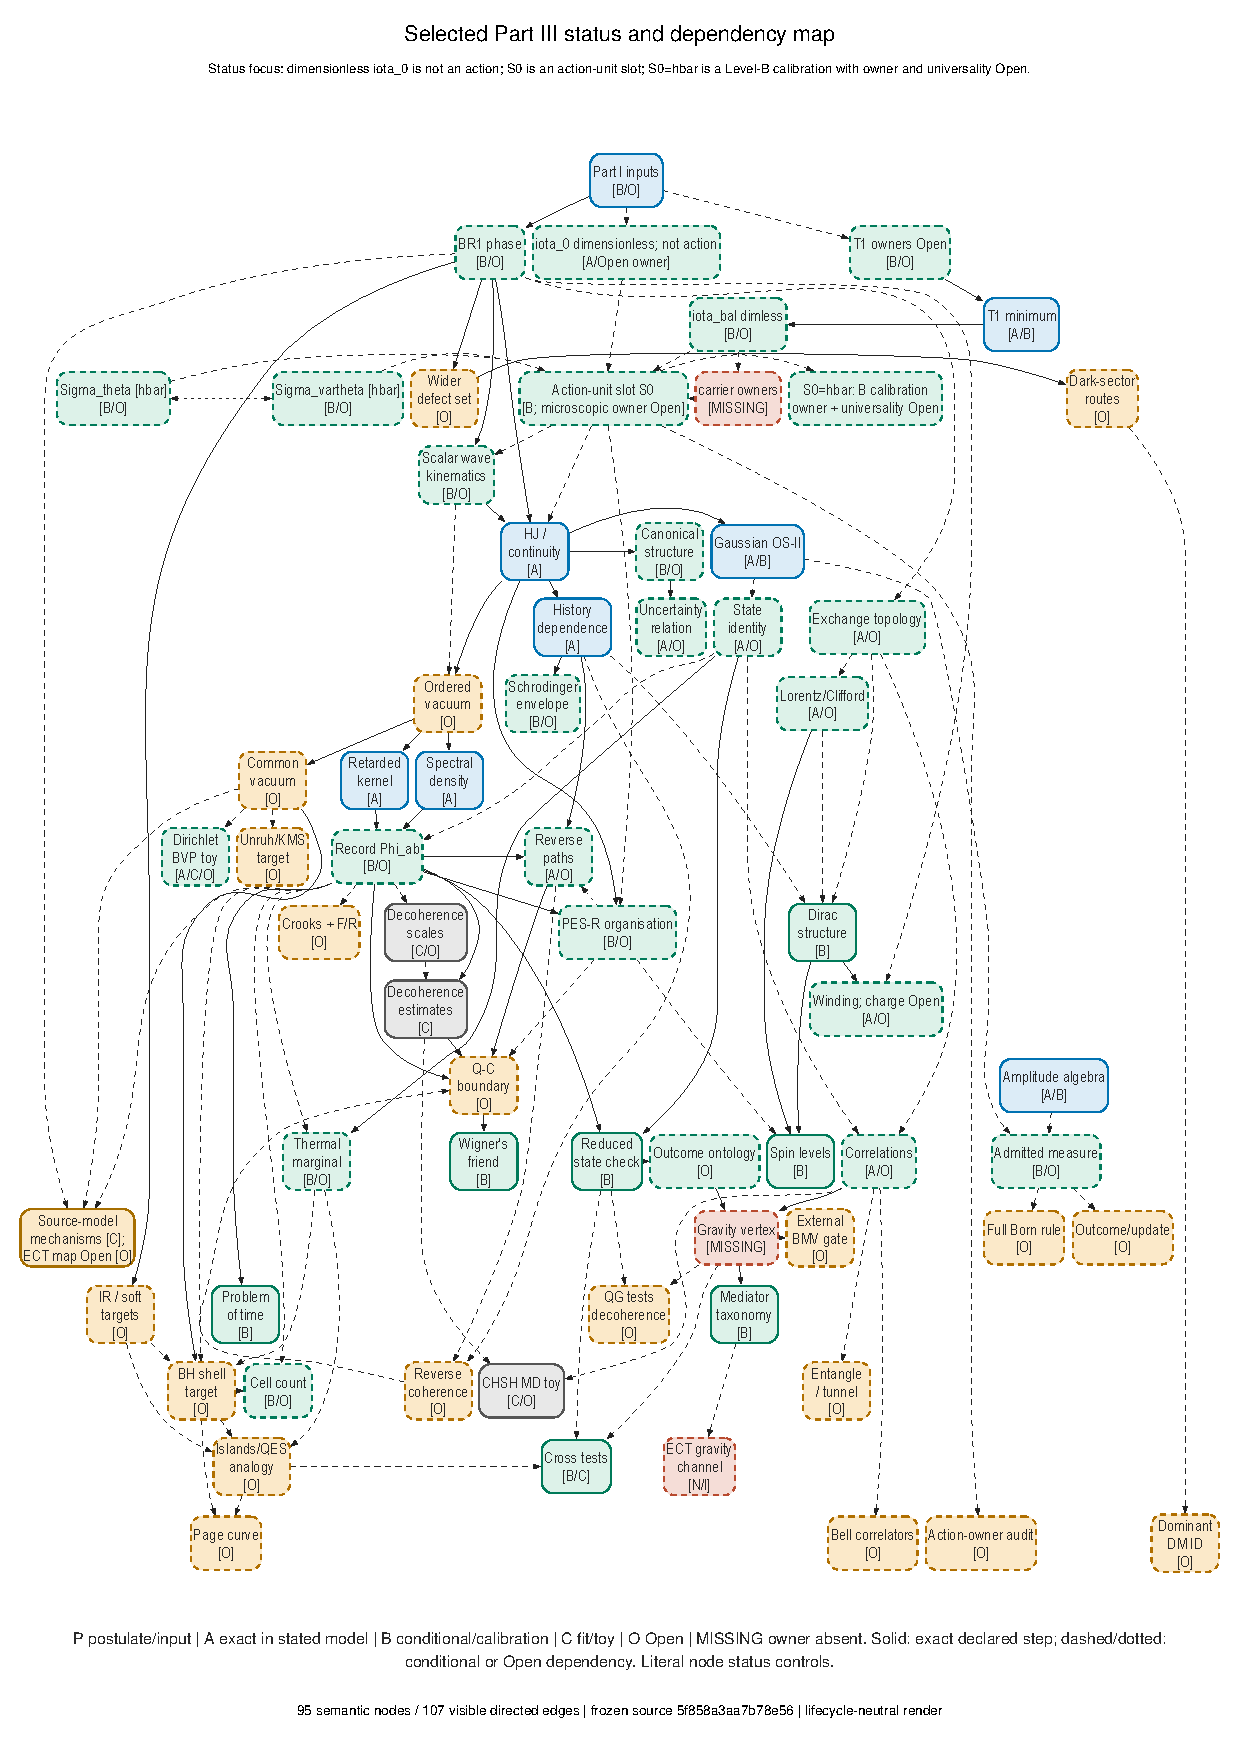
\includepdf[
  pages=1,
  fitpaper=true,
  pagecommand={\thispagestyle{empty}}
]{../figures/r185/logic_maps/partIII_status_dependency.pdf}
\clearpage

\part{Summary, Comparisons, and Outlook}
\label{part:summary_pop}


\section{Architectural comparison with neighbouring programmes}

ECT is not the only attempt to address the foundational questions of physics. The following comparison locates it among its closest architectural neighbours.

\textbf{General Relativity + Standard Model:} Time and Lorentzian structure
are supplied.  The Standard-Model gauge/matter content is input.  In standard
$\Lambda$CDM applications, cold dark matter is an additional non-SM
component and late acceleration is modelled by $\Lambda$.  The black-hole
information problem remains open.

\textbf{Einstein--aether theory (Jacobson, 2004):} Lorentzian structure is fundamental; a preferred frame is added via a postulated unit vector $u^A$. In ECT, $n^A=\partial^A\Phi/|\partial\Phi|$ is a kinematic identity wherever the gradient is nonzero, but P4 supplies its aligned background value; a physical state and its selection are not derived.

\textbf{Ho\v{r}ava--Lifshitz gravity:} Lorentzian spacetime is supplied and
high-energy Lorentz invariance is broken explicitly.  ECT instead starts
from Euclidean $O(4)$ and P4 supplies a nonzero-vector direction whose
stabiliser is $O(3)$; the physical ordered state and spontaneous selection
remain Open;
the scalar principal tensor is Lorentzian only when the supplied
coefficients obey $\beta(\beta-\alpha)<0$; on the retained
$\beta>0$ branch this is $\alpha>\beta>0$.  A physical metric remains Open.

\textbf{Volovik's ``Universe in a Helium Droplet'':} Condensate analogies motivate emergent geometry.  ECT conditionally classifies one supplied scalar principal tensor as hyperbolic, while physical branch selection and gravity remain Open.

\textbf{Causal Dynamical Triangulations:} Lorentzian structure is imposed as a lattice constraint. In ECT, residual symmetry classifies the supplied scalar principal tensor as Lorentzian iff $\beta(\beta-\alpha)<0$ (equivalently $\alpha>\beta>0$ only on the retained $\beta>0$ component); SSB does not select that inequality or a physical universal cone.

\textbf{Hartle--Hawking no-boundary proposal:} The proposal defines a quantum
state through a path integral (or semiclassical saddles) over regular compact
positive-definite or complex four-geometries.  It does not posit ECT's
Euclidean scalar medium.

\textbf{MOND (Milgrom, 1983):} The critical acceleration $a_M$ is introduced as a universal free constant. In practical functional G the corresponding scale is fitted and compared with $cH_0/(2\pi)$; its microscopic origin and any environment/history law remain Open. The characteristic acceleration and the fitted HRC response are Level~C inputs; the BTFR slope is conditional B/C algebra inside that functional, while a universal environment law remains Open.

\textbf{Superfluid dark matter models:} Spacetime is pre-existing; a
superfluid component is added as dark matter.  In ECT, physical spacetime
descent and medium response are investigated within one architecture, but
the physical metric remains Open.

ECT places these sectors within one condensate architecture while classifying every link separately as structural, closure-level, fit-level, or Open; it does not derive every compared structure from the minimal action.


\section{Distinctive features of the framework}

Features emphasised by the present ECT programme include:

\textbf{Single-condensate architecture:} Spacetime, gravitational response, quantum-theoretic structure, gauge-sector routes, and dark-sector phenomenology are all placed within one scalar-condensate architecture, but with different logical status: some parts are strict structural consequences, some are closure-level reconstructions, and others remain open completion targets.

\textbf{No external time in the bare model:} P4 adopts the physically relevant ordered direction, and the declared scalar EFT admits a candidate coordinate $x^0=w$.  Physical clocks, rods and time observables are not derived by symmetry breaking alone and remain Open.

\textbf{Mechanism programme:} compact phase, verified reflection-positive subsectors and the Euclidean boundary-value formulation supply distinct conditional inputs; they do not jointly derive the complex law, operator algebra, probability measure or physical clock behind selected quantum equations; exact Born, measurement, interacting operator, and matter completions remain Open.

\textbf{Honest epistemology:} Every result is classified as Level~A, B, C, or Open; the status ceiling controls the prose.

\textbf{Cross-sector action-scale programme:} The phase-only fixed-core $\iota_0^{\rm EFT}$, BR1 phase-tension $\iota_{0,\rm bal}^{\rm eff}$ and texture-worldline modulus coefficient $\iota_{0,\rm bal}^{(\vartheta)}$ are not interchangeable definitions.  CDE-$\Phi$ is only a post-order acceptance criterion; it does not choose among them.  Reuse in independently owned wave and canonical closures is provisional.  Compact winding derives none of their finite physical values, common normalisation or identification with $\hbar$.  The candidates do not generate probability: the complete applicable corrected OS-II package conditionally supplies a Hilbert space only in verified subsectors, ordinary Gleason constrains a supplied normalized noncontextual countably additive projector measure only at complex dimension at least three (with a separate Busch effect/POVM or named qubit extension), and only a specified source-model channel can suppress selected coherences.  A completed derivation must first establish one 4D action/state/profile/subtraction/quotient owner, proper-time ensemble, Hessian and barrier, then prove any relation among the reduced coefficients, and finally show that independently normalised sectors use the same physical action scale.  Incompatible normalisations would falsify universality, not the algebraic existence of a sector-specific minimum.

\textbf{Dark-sector application scope:} The adopted galactic fit has no particle-halo term and the late-time diagnostic closure has no rigid external cosmological constant.  These are closure choices: they neither derive all dark-sector phenomena from the scalar action nor exclude hidden-sector particles.

\textbf{Common pre-geometric research programme:} A conditional scalar characteristic geometry, an Abelian-connection programme, algebraic weak-sector ingredients, the adopted Level-B P7 rank-three bundle postulate with fibrewise $SU(3)$ reduction and an Open physical-colour map, and a candidate director EFT operator are organised in one framework but have different status.  P7 is not a necessary or unique physical colour completion; that identification remains Open. Physical gravity, local gauge bundles and actions, matter representations, weak chirality, the director coefficient and observable magnitudes remain Open.  This broad scope is an organising feature, not a derivation or unification theorem.

\textbf{Director coupling:} The stated EFT basis conditionally admits a lowest-dimension homogeneous vector-current operator (B), whose coefficient may vanish.  It is a density term, not a spin interaction or source-generated fifth force.  Relative vector-current observables require a non-universal/gradient/curvature map; spin and composition-dependent force signals require separate operator and source/body completions.  All physical magnitudes remain Open.

\textbf{Minimal displayed parameter inventory:} P3 contains the two potential
couplings $(\mu^2,\lambda)$, equivalently $(\phi_0,\lambda)$; P4 separately
supplies the dimension-two gradient datum $u_0$; and the scalar principal
operator separately uses the dimensionless coefficients $(\alpha,\beta)$.
The choice $(\alpha,\beta)=(2,1)$ combines a Level-B unit-slope benchmark with
a normalisation convention; it does not reduce the complete ECT
input/owner count to two scales.  Action magnitudes, states, matching
coefficients, sector operators and observable maps remain additional
completion data.  No irreducible parameter count is claimed until those
owners and their relations are derived.


\section{Status map: standard structures, conditional ECT reconstructions, and Open programmes}
\label{sec:pop_postulates_reinterpreted}

This section juxtaposes standard structures with several logically
different ECT entries: theorem-level results inside supplied models,
conditional reconstruction routes, imported calibration or source-model
relations, phenomenological benchmarks, and Open physical owners.  Inclusion
in one table does not make every row an ECT consequence or give the rows
uniform evidential strength.  The following compact status map retains the
most representative cases. A full version with all entries and
section references is given in the technical preprint
(\S\ref{sec:pop_postulates_reinterpreted} corresponds to the
preprint's ``Comprehensive map''; see there for the extended seven-group
classification). Status labels: A = an exact result inside the explicitly
declared model and assumptions with a reproducible derivation; B = a
structural/conditional derivation or closure route with an explicit Open
matching, identification or physical-owner step; C = a phenomenological fit,
proxy, benchmark or application-level estimate; Open = not established.

\renewcommand{\arraystretch}{1.15}
\begin{longtable}{@{}p{4.5cm}p{2.5cm}p{4.7cm}p{2.2cm}@{}}
\caption*{\textbf{Standard structures, conditional ECT reconstructions, and Open programmes (mixed-status map).}}\\[-4pt]
\toprule
Standard structure & Conventional status & ECT result, route, or missing owner & Level \\
\midrule
\endfirsthead
\toprule
Standard physics (cont.) & Status there & ECT origin & Level \\
\midrule
\endhead
\bottomrule
\endfoot
\multicolumn{4}{@{}l}{\textbf{Foundations and spacetime}}\\
\midrule
Lorentzian scalar signature $(-,+,+,+)$ & Fundamental input & Classified iff supplied $\beta(\beta-\alpha)<0$; retained shorthand $\alpha>\beta>0$ only for $\beta>0$; P4/SSB does not select the branch & A-math conditional / Open \\
Time as a distinguished direction & Fundamental & P4 supplies the ordered direction $w$; a physical time/clock requires the branch, lapse and matter/metric maps & postulate/Open \\
Arrow of time / second law & Open / empirical & Retarded response does not fix entropy sign; ECT reduced channel, entropy functional, and detailed-balance/contractivity hypotheses remain Open & Open \\
Scalar slope / physical speed & Fundamental speed constant & $\hat c_*^2=\beta/(\alpha-\beta)$ is dimensionless; $c_{\rm char}=c_{\rm u}\hat c_*/\mathcal N_\Phi$ uses the clock map and $c_{\rm char}=c$ is the adopted scalar-clock calibration, while photon/tensor cone equality remains Open & A-math / B calibration / Open cone universality \\
Newton's constant $G_N$ & Fundamental constant & Conditional EFT identity
$G_N^{\rm nat}=(8\pi M_G^2)^{-1}$ after a physical tensor normalisation is
supplied; microscopic map and response matching Open & B conditional / Open owner \\
Reduced Planck constant $\hbar$ and ordinary Planck constant $h_{\rm P}$ & Fundamental constants related by $h_{\rm P}=2\pi\hbar$ & Supplied reductions distinguish $\iota_0^{\rm EFT}$, $\iota_{0,\rm bal}^{\rm eff}$ and the texture-worldline $\iota_{0,\rm bal}^{(\vartheta)}$; a conditional owner map plus the explicit Level-B physical calibration $S_0=\hbar$ give $\Sigma_\vartheta\mathcal I_{1,\min}=h_{\rm P}$ only in the bending-free $n=1$ branch.  The common 4D owner, proper-time ensemble, stability, absolute derivation and cross-sector universality remain Open & A-math in supplied models / B route and calibration / Open ownership and derivation \\
\midrule
\multicolumn{4}{@{}l}{\textbf{Quantum mechanics postulates}}\\
\midrule
Complex Hilbert space / superposition & Axioms & Corrected OS-II reconstruction only after the full measure/correlator, algebra/reflection, regularity/growth, covariance, RP, symmetry and applicable locality/cluster hypotheses are supplied; Gaussian/free kernels verify only their declared subset & A-math conditional / Open ECT \\
Schr\"odinger equation & Axiom & Leading conditional NR envelope after a separate norm-preserving complex law, Hamiltonian/domain, state/stable KG positive-frequency component, the same physical clock, mass matching, weak interaction, slow-envelope regime and residual control are supplied; no generic descent from the real scalar action & A-math asymptotic / B--Open owner \\
Planck--Einstein relation $E=\hbar\omega$ & Quantum postulate / empirical identification & A supplied stationary eigenproblem gives $E=S_0\omega$; the Hamiltonian, clock and finite coefficient require an owner, and $S_0=\hbar$ is the separate Level~B empirical calibration & B calibration / Open owner \\
Canonical commutator $[\hat q,\hat p]=i\hbar$ & Postulate & Conditional only after a Hilbert representation, self-adjoint domains and commutator are supplied; compact winding does not fix the same $S_0$ normalisation & B/Open \\
Projective measurement / update rule & Textbook operational axiom; ontological collapse is interpretation-dependent & Specified source-model dephasing can suppress selected coherences after coupling, state, kernel, trace and timescale are supplied; physical ECT channel, probability, pointer, outcome and update remain Open & Open \\
Born rule $P=|\psi|^2$ & Postulate & Ordinary Gleason: complex $\dim\mathcal H\ge3$ plus supplied normalized noncontextual countably additive projector measure; qubit requires supplied Busch effect/POVM or named composite extension.  Physical measure/state/event map, outcome and update remain Open & A-math conditional / Open ECT \\
Pauli exclusion principle & Nonrelativistic fermionic antisymmetry postulate; relativistic spin--statistics consequence under standard hypotheses & Free-kernel antisymmetric OS consistency is mathematical A; application to a physical ECT spinor/CAR sector is B/Open & A-math / B--Open \\
Dirac equation & Postulated fermion dynamics & Conditional only in the supplied irreducible four-complex-component Clifford-factorisation class with physical metric/tetrad, spin structure, local linear Lorentz covariance and exact KG factorisation; reducible, constrained/gauge and non-Clifford systems are outside & A-math conditional / physical ECT spinor Open \\
\midrule
\multicolumn{4}{@{}l}{\textbf{Gauge sector}}\\
\midrule
Abelian gauge sector & Postulated gauge principle & Compact phase supplies winding and a conditional connection/Maxwell candidate; gauge reduction, physical $U(1)_{\rm em}$, unbroken photon, charges and matter map remain Open & B/Open \\
Weak-sector structure & Postulated chiral $SU(2)_L$ & Orientation-sector $SU(2)$ lift plus Hopf-fibered phase--orientation locking gives a candidate pre-gauge geometry with three broken directions; local chiral $SU(2)_L$, hypercharge, $g,g'$ and $\theta_W$ remain open & B/Open \\
Neutrino masses and mixing & Seesaw / Dirac / Majorana (model-dependent) & Standard one-flavour seesaw and Weinberg-operator normalisations hold after their masses, coefficients and flavour content are supplied; ECT derives none of those owners; PMNS/MSW may be supplied & A-math conditional / Open ECT \\
$SU(3)$ colour sector & Postulated colour symmetry & Direct injective embedding in the displayed minimal algebra is excluded by dimension; P7 is an adopted positive-definite Hermitian frame postulate, while alternative completion classes and physical colour remain Open & A restricted / B input / Open colour \\
\midrule
\multicolumn{4}{@{}l}{\textbf{Gravity, cosmology, vacuum}}\\
\midrule
Metric/gravity route & Einstein equations postulated in GR & Scalar-only metric equation holds inside its Level-B ansatz; only at fixed $\alpha,\beta$, about homogeneous $\bar n=w$, and at tangent-director linear order does the fixed image have only $h_{iw}$ and no linear TT/static-density seed; quadratic/nonlinear/composite routes and an independent tensor action, source and metric/photon map remain Open & A no-go in fixed map / Open completion \\
Candidate anisotropic proxy $\mathcal X^{\rm cand}_{\mu\nu}[n]$ & Absent in GR & External proxy only; physical $T^{(n)}_{\mu\nu}$ requires covariant $S_n[g,n,\lambda_n]$ & C/Open \\
Late-time acceleration ($\Lambda$) & Postulated constant &
Regular two-slope scalar proof of class; physical ECT source and state Open & A conditional / C benchmark / Open ECT \\
Vacuum-offset problem & Standard UV--IR vacuum-energy mismatch (often summarised as up to $10^{120}$ in a Planck-density comparison) & Exact orientation determinant does not derive decoupling; a separately supplied trace-free action is classically shift covariant through $V+C_I$ & External order-of-magnitude framing / A inside supplied completion; ECT action map Open \\
Observed late source & Empirical fitted density & $3\Omega_{\rm late,0}^{(\rm GR\,ref)}\bar M_{\rm Pl}^2H_0^2$ is a GR-reference convention after the metric and Planck calibration are fixed; the generic scalar--tensor constraint also contains $F_0,\dot F_0$ and any orientation stress & State/matching datum; ECT owner Open \\
Particle dark matter (galactic fit channel) & Postulated halo & HRC-only algebraic diagnostics are recomputed (C); BTFR slope 4 is conditional on the separate bridge (B/Open) & C / B--C \\
Casimir / Unruh / Hawking sector & QFT vacuum/observer effects & Supplied scalar-BVP and standard QFT target calculations are A mathematics/A external; physical ECT fields, metric, state, boundary/detector coupling and strong-field owners remain Open & A mathematics/external / Open ECT \\
\midrule
\multicolumn{4}{@{}l}{\textbf{Long-standing mysteries and targets}}\\
\midrule
Fine-structure constant $\alpha_{\rm fs}=1/137$ & Fundamental constant &
The standard identity $\alpha_{\rm fs}=q^2/(4\pi Z_A)$ is conditional on a
normalised photon and charge; ECT supplies neither the physical photon nor the
electroweak/matter matching owner & External identity / Open ECT \\
Three fermion generations & Empirical input & A supplied one-dimensional
well has tunable bound-state counting, but no physical Dirac operator,
family map or parameter owner is derived & A toy mathematics / Open ECT \\
Proton stability & Empirical lower bounds / model-dependent rules & Three conditional patterns; P7/triality supplies no $U(1)_B$, while $\Lambda_B$, mediators and coefficients remain Open; only standard conditional EFT scaling is retained & External constraint / Open ECT \\
Baryon asymmetry $\eta_B$ & Sakharov + model & External observational target
and missing-owner inventory;
the baryon current/violating vertex, nonzero CP source and state, transition,
transport, washout and ECT-native derivation remain Open & Open ECT \\
Quantum gravity (UV/spin-2 closure) & Open problem & Scalar characteristic and quantum/open-system routes share an architecture; physical tensor, canonical scale, source and RP/OS reconstruction remain Open & Open \\
Measurement problem & Open problem & A specified source model can dephase selected alternatives, but dephasing is not a Gleason premise.  The probability measure/state/event map, physical ECT channel, pointer, outcome and update have separate Open owners & Open \\
\end{longtable}

The compact table is a selective index, not a proof by unification.
The full preprint adds reflection-positivity details, quantum-statistics
conditions, the fixed-map tensor no-go and completion gates, conditional
Klein--Gordon and Crooks routes, cosmological and lensing programmes,
neutrino benchmarks, the orientation-determinant lemma, the separately
supplied trace-free completion, the regular two-slope proof of class, and the
Open physical action/state map.  Each row must be read at its printed level:
standard mathematics reproduced in a supplied model, an external result, or
a fit is not automatically evidence for ECT.  The useful architectural claim
is narrower: these owners and missing bridges are organised in one auditable
programme without presenting them as equally derived.

\section{Key equations, laws, and principles of ECT}

The following is a status-separated equation and owner inventory.  It mixes
supplied actions, conditional mathematics, external formulae, fitted
diagnostics and Open targets; inclusion in the list does not make an item a
derived quantitative prediction of ECT.

\textbf{Foundational action:}
$\mathcal I_E^{\rm P3}=\int d^4X\{
\frac12(\partial_A\Phi)^2+V(\Phi)\}$ is dimensionless;
$S_E^{{\rm P3},{\rm phys}}=A_{\rm P3}\mathcal I_E^{\rm P3}$ and
$d\mu_{\rm P3}\propto
e^{-\kappa_{\rm P3}\mathcal I_E^{\rm P3}}\mathcal D\Phi$ with
$\kappa_{\rm P3}=A_{\rm P3}/\Sigma_{\rm PI,P3}>0$.  Here
$V=-\mu^2\Phi^2/2+\lambda\Phi^4/4$; the two positive action owners and their
maps to quantum-sector scales are Open.

\textbf{Supplied P4 nonzero-gradient datum:}
$\langle\partial_A\Phi\rangle = u_0\,\delta_{Aw}$; the nonzero vector has stabiliser $O(3)$.  The brackets denote the declared coarse-grained datum; a stationary physical vacuum and spontaneous $O(4)\to O(3)$ selection remain Open.

\textbf{Conditional scalar principal tensor:}
$K^{AB} = \beta\,\delta^{AB} - \alpha\,n^An^B$.  This local algebraic basis is unique only inside the supplied scalar-operator inventory; the coefficients, their realised sign domain and the physical action owner are independent inputs.

\textbf{Scalar slope and physical speed:}
$\hat c_*^2=\beta/(\alpha-\beta)$ and $c_{\rm char}=c_{\rm u}\hat c_*/\mathcal N_\Phi$; $c_{\rm char}=c$ is the adopted Level-B scalar-clock calibration, while $c_\gamma=c_{\rm char}$ remains Open.

\textbf{Matching relations:}
$G_N^{\rm nat}=(8\pi M_G^2)^{-1}$ is the separate tensor matching;
$S_0=\hbar$ is the adopted Level-B action calibration; and
$\phi_0=\zeta_\phi\bar M_{\rm Pl}$, $\zeta_\phi>0$,
$\zeta_\phi=O(1)$, is an independent Level-B scale ansatz.  Their microscopic
owners and universality remain Open.

\textbf{Cross-sector cone universality:}
The scalar and supplied phase truncations share only their common-length slope through $K^{AB}$; $c_{\rm phase}=c_{\rm char}$ requires the same supplied clock/lapse map on the aligned frozen-coefficient patch.  The identifications $c_\gamma=c_{\rm char}$ and $c_{\rm GW}=c$ remain Open completion gates.

\textbf{Loop quantisation:}
$\oint \partial_A\theta\,dX^A=2\pi n$ after BR1 is supplied; \quad $\iota_{\rm elem}^{\rm(fixed\ core)}=2\pi \iota_0^{\rm EFT}$ in the phase-only closure.  A distinct texture-worldline modulus reduction can define $\iota_{0,\rm bal}^{(\vartheta)}=\sqrt{2K_\vartheta^{1\mathrm D}\mathcal T_{\rm loop}}$ only after its common owner and proper-time ensemble are supplied; it equals the BR1 phase-tension coefficient only if the modulus/stiffness map is proved.  With the explicit Level-B calibration, the bending-free $n=1$ branch gives $\Sigma_\vartheta\mathcal I_{1,\min}=h_{\rm P}$; profile/Hessian, bending/barrier, microscopic ownership and stability/universality remain Open.

\textbf{Entropy-production status:}
the retarded backbone and positive pairwise noise are structural, but a monotone entropy theorem requires a declared reduced channel, entropy functional, stationary state, and detailed-balance/contractivity assumptions; no universal scalar rate follows.

\textbf{Generalised Einstein equations:}
$F G_{\mu\nu}=8\pi G_N T_{\mu\nu}/c^4+\mathcal T^{(q)}_{\mu\nu}$ in the scalar-only undivided convention; division by $F$ adds no orientation term, and $T^{(n)}_{\mu\nu}$ requires a separate covariant $S_n[g,n,\lambda_n]$ (Open).

\textbf{HRC algebraic relation:}
$g_N=\mu_{g,k}(g^2/a_M^2)g$, $k\in\{0,3\}$.

\textbf{BTFR:}
$v_{\rm flat}^4 = G_N M_{\rm bar}\,a_M$ (slope~4, algebraic).

\textbf{Hubble evolution:}
$t_{0,\rm ECT}=\int_{a_{\rm ord}}^1 da/[aH_{\rm ECT}(a)]$; the named two-slope state gives $\tau_{2s}\equiv H_{2s}(0)\Delta t=0.96368678$ conditionally. A dimensional age uses the declared $H_{2s}(0)=H_0^{\rm cal}$ calibration; the physical observable map and microscopic selection remain Open.

\textbf{PES-R inventory:}
Action stationarity, pairwise record stability, finite-time sector diagnostics, and phase admissibility are separate objects; no universal intersection theorem is claimed.

\textbf{Source-model visibility proxy:}
$\tau_{\rm vis}=1/(N_{\rm eff}\gamma)$ only for a declared channel, state,
rate convention and observation protocol; it is not a universal ECT
decoherence time or sector boundary.

\textbf{BH entropy target:}
$S_{\rm BH}=A/(4\ell_{\rm Pl}^2)$ is an external target; the current ECT action derives neither a physical black-hole area law nor the coefficient $1/4$.

\textbf{Casimir (conditional):}
For a separately supplied three-independent-scalar Dirichlet BVP with
the physical light speed, $F_{N=3}^{\rm scalar}=\tfrac32F_{\rm QED}$
arithmetically.  ECT does not derive that mode bundle, material boundary,
stress observable or force coefficient.


\section{Conditional completion tests, fitted diagnostics, and Open observational handles}
\label{sec:pop_predictions}

ECT claims are separated into structural discriminants, conditional
completion tests and explicitly Open observables.  The named two-slope
scalar--tensor action/state gives a conditional background, age and
restricted diagnostic estimates, but P1--P6 do not uniquely select that
completion.  Physical Hubble inference, JWST forward modelling,
gauge-complete growth and ISW, and lensing remain owner-specific Open
programmes:

\begin{enumerate}
\item \textbf{BTFR slope = 4 within the adopted galactic closure} (\emph{B/C, conditional}). This is an algebraic consequence of the assumed deep branch. A robust systematic deviation would challenge this closure rather than the entire ECT framework.

\item \textbf{$a_M \sim cH_0/(2\pi)$} (\emph{Level~C matched
comparison/input}). Its empirical comparison is meaningful, but its
microscopic ECT origin and environment/redshift law remain Open.

\item \textbf{Director-coupling completion} (\emph{Open}).  The fixed vector spurion supplies neither a source-generated force nor an E\"otv\"os window.  MICROSCOPE constrains a future completion only after its field/profile, species/body charges, range and screening map are declared.

\item \textbf{Late-time acceleration.} Minimal P1--P6 and the
positive-kinetic stress lemma do not select the physical source or $w(a)$.
The named two-slope completion supplies a regular conditional history; its
microscopic selection, physical metric/state map and likelihood remain Open.

\item \textbf{Exploratory environment/history law $\Xi$ for $a_{M,\rm eff}$} (\emph{Open}). No sign or amplitude is predicted. A null result rejects only the declared $\Xi$ ansatz; a correlation would motivate, but would not derive, an ECT mechanism.

\item \textbf{Casimir boundary-response programme} (\emph{A mathematics/Open ECT}). The supplied $N$-scalar Dirichlet BVP is exact and its separately supplied $N=3$ case retains the $3/2$ toy identity, but the physical ECT mode bundle, material boundary map, stress observable and force are not derived.  No ECT $3/2$ correction is predicted.

\item \textbf{Tensor polarisation gate} (\emph{Open}). At fixed $\alpha,\beta$, about homogeneous $\bar n=w$, and at tangent-director linear order, the fixed image has no linear TT sector; nonlinear/composite/additional-field routes remain Open.  A separately supplied massless Fierz--Pauli completion would have two TT modes; observed extra polarisations would reject that completion, not the present negative theorem.

\item \textbf{No particle-halo term in the specified galactic fit} (\emph{C}). A confirmed particle component required by rotation-curve and RAR/BTFR data would challenge that closure; discovery of a hidden-sector particle would not by itself falsify ECT.

\item \textbf{Bare scalar-ratio identity.} With $K_\phi^{\rm phys}=\bar M_{\rm Pl}^2\omega\dot\phi^2/2$ and a positive bare denominator, the supplied pieces have $w_\phi^{\rm bare}\ge-1$.  Non-minimal $F$-derivative terms leave observable $w_{\rm eff}(a)$ unconstrained; a falsifier exists only for a complete model that predicts the same observable history.

\item \textbf{Propagation corrections} (\emph{Open}).  Photon LIV is not an
operational ECT prediction: Fermi--LAT constrains specified external
dispersion and source-lag models, which become an ECT gate only after a
physical photon operator, coefficient, suppression scale, clock and forward
likelihood map are derived.  Tensor dispersion and delay likewise remain Open
until their physical operator, coefficient, scale and observable map are
owned.

\item \textbf{Proton stability} (\emph{Open ECT}).  Conditional on a completed
gauge/flavour action, three selection-rule patterns remain possible: full
low-energy protection, partial protection with $\Delta B=1$ forbidden, or
generic $\Delta B=1$ violation.  In the last case
$\tau_p\propto\Lambda_B^4/(|C_B|^2m_p^5)$ is the usual dimension-six NDA
scaling, up to channel-dependent hadronic, renormalisation-group and
phase-space factors.  P7 fixes
neither $\Lambda_B$, $C_B$ nor the mediator spectrum; current experimental
bounds~\cite{SuperK2020} constrain any named completion.
\end{enumerate}

\paragraph{Near-future observational gates for future completions.}
Beyond the conditional or externally constrained handles already accessible
with current data, several observational programmes expected to deliver
future results can constrain named ECT completions once their action, state
and observable maps are supplied.
\emph{(i)}~Full-sky CMB polarisation missions such as LiteBIRD can test
whether the primordial
tensor spectrum is compatible with any viable condensate-based
early-Universe completion of ECT\@.
\emph{(ii)}~Combined CMB, weak-lensing and large-scale-structure
measurements from programmes such as the Simons Observatory, Euclid and
Rubin/LSST can probe
whether a completed action-owned scalar--metric background and perturbation
response, together with an explicitly external anisotropic proxy
$\mathcal X^{\rm cand}_{\mu\nu}[n]$, leaves a detectable signature in the
lensing--growth consistency relation.  The divided coefficient
$G_{\rm div}(z)$ alone is not such a prediction.
\emph{(iii)}~Space-based gravitational-wave detection will constrain a future ECT tensor completion through its propagation cone, polarisation content and damping law.  The tested fixed-$\alpha,\beta$ tangent-director linear map predicts neither two TT modes nor $c_{\rm GW}$; untested nonlinear/composite routes remain Open.  Standard-siren determinations of $H_0$ remain external cosmological data rather than tests of a derived tensor prediction.
A detailed table of near-future discriminants, with explicit
ECT statements and falsification verdicts, is given in the
technical preprint.

\paragraph{ISW and lensing target.}
An ECT prediction requires the time-dependent Weyl potential of the physical
photon metric, obtained from a gauge-reduced perturbation action on the same
background.  A restricted same-metric, zero-slip, sub-horizon proxy gives only
$0.00267$--$0.00292\%$ Weyl-carrier and $0.00308$--$0.00813\%$
conformal-derivative changes over $0\le z\le2$ for the named near-GR state.
It is not an ISW amplitude or lensing spectrum; those full observables remain
Open.

\section{Colour completion: adopted P7 structure and Open physical owners}
\label{sec:pop_colour}

Part~IV of the technical preprint does not derive physical colour from
P1--P6.  The exact dimension inequality
$\dim\mathfrak{su}(3)=8>6=\dim\mathfrak{so}(4)$ excludes only a direct
Lie-subalgebra embedding into the displayed $O(4)$ order-parameter algebra.
Reducible-singlet, emergent/nonlinear, independently supplied bundle and
defect-kernel routes remain possible.

\paragraph{P7 is an adopted structural postulate.}
In addition to P1--P6, P7 adopts a global complex rank-three vector bundle
$\mathcal C\to\mathcal M^4$ with transition cocycle, a positive-definite
Hermitian form $h$ and a compatible nowhere-vanishing complex volume form
$\Omega$ normalized by $|\Omega|_h=1$.  The fibrewise stabilizer of
$(h,\Omega)$, equivalently the reduced structure group, is $SU(3)$; this is
Level-A mathematics conditional on the supplied bundle data.  Global
structure-preserving automorphisms form the associated gauge group of sections
and are not one finite-dimensional copy of $SU(3)$.  P7 is a reverse-engineered
Level-B structural input, not a P1--P6 descent theorem and not a necessary or
unique completion.  The abstract reduction admits compatible mathematical
connections under the usual bundle assumptions, but P7 selects none as the
physical dynamical connection and does not identify the structure with
physical colour.  The physical colour connection, Yang--Mills action, measure,
matter representations, couplings, spectrum and QCD map remain Open.

\paragraph{Scoped structural consequences.}
A nonzero fundamental $\mathbf3$ VEV has stabiliser $SU(2)$, whereas a
reducible representation can contain an invariant singlet.  A Proca mass is
forbidden only after an exact gauge theory is independently supplied, and
the P7 fields themselves provide no colour-charged Higgs.  An internal
oscillator tower is not identified with a physical glueball spectrum without
a gauge-invariant operator, constraints and dynamics; this is
non-identification, not a universal spectrum no-go.

\paragraph{Baryon and proton firewall.}
The invariant $\varepsilon_{abc}q^aq^bq^c$ permits a baryon-like colour
singlet, but colour triality does not derive $U(1)_B$, baryon charges, a
current or a baryon-violating vertex.  The three proton-selection patterns
remain conditional on a full gauge/flavour action.  In the generic
dimension-six pattern,
$\tau_p\propto\Lambda_B^4/(|C_B|^2m_p^5)$ is the usual NDA scaling, up to
channel-dependent hadronic, renormalisation-group and phase-space factors.  A
named C/Open reference branch may set $\Lambda_B=c_B\phi_0$ and retain $C_B$
as an independent coefficient; $c_B=|C_B|=\zeta_\phi=1$ gives only the
crude unit-coefficient NDA reference $\tau_p\sim1.01\times10^{42}$\,yr, while
a protecting symmetry may give $C_B=0$.  Hadronic, RG, flavour, phase-space
and normalisation owners are omitted at that point.  P7 fixes none of these
inputs, so no proton lifetime is predicted; experimental bounds constrain
each named completion.

\paragraph{Source-model RG and strong CP.}
The familiar $b_0=11$ running is reproduced only on the separately declared
constant, $Y_0=0$, CP-even, matter-free pure-$SU(3)$ source branch.  General
anisotropic running is multi-coefficient and Open.  The physical strong-CP
parameter is
$\bar\theta\equiv\theta_{\rm gauge}+\arg\det M_q\pmod{2\pi}$ when
$\det M_q\ne0$.  In a massless-quark limit the determinant phase is
ill-defined/removable and must be treated separately.  P7 supplies neither
mass matrix nor relaxation mechanism, so the problem is reopened, not solved.

\paragraph{Mass-gap statement retained conditionally and framework hypothesis
$H_{\rm Clay}$.}
A positive global gap follows from the stated external transfer theorem only
after a fully specified reflection-positive colour theory has a unique
vacuum, positive adjointed/reflected forms, a transfer-cyclic dense physical
class, uniform exponential decay and a positive two-sided scale map.  The
local HKLoc bookkeeping supplies none of these global owners.  Separately,
ECT adopts the Level-B/Open framework hypothesis $H_{\rm Clay}$ that a future
P7 physical-colour completion may be emergent and finite-cutoff rather than
the primitive continuum object in the Clay statement.  This hypothesis is
not a consequence of P7, requires a colour action, measure, regulator and
scale map, supplies no evidence against continuum Yang--Mills, and is neither
a solution nor a dismissal of the Clay problem.  Physical colour,
confinement, the glueball spectrum and an ECT-owned mass gap remain Open.

\begin{figure}[H]
\caption{Complete Part~IV structural logic.  Solid statements are scoped
group/source-model algebra; dashed dependencies lead to the adopted Level-B
P7 structural input and Open physical colour, baryon/proton, strong-CP and
mass-gap owners.  No arrow turns P7 into a P1--P6 forward derivation or into a
physical-colour result.}
\label{fig:pop_partIV_logic}
\end{figure}

\clearpage
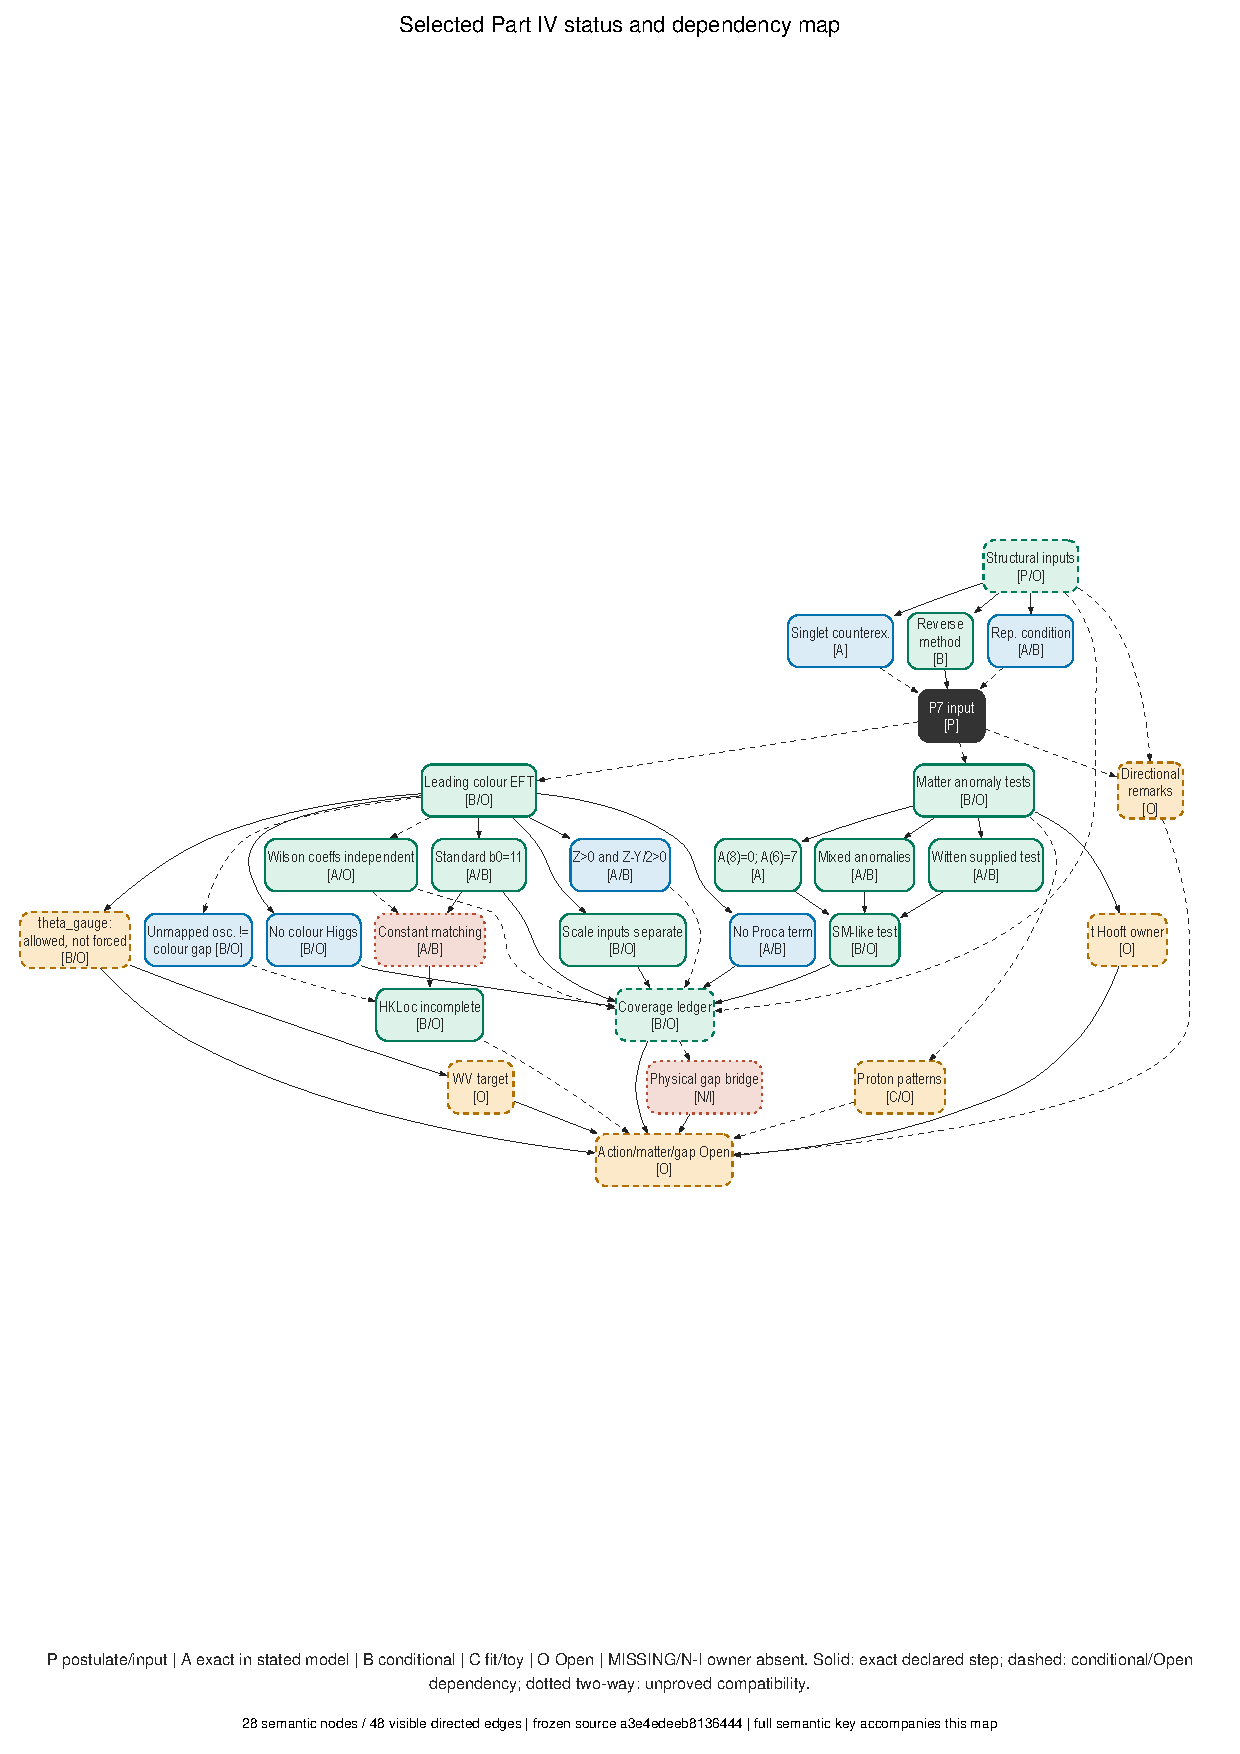
\includepdf[
  pages=1,
  fitpaper=true,
  pagecommand={\thispagestyle{empty}}
]{../figures/r185/logic_maps/partIV_status_dependency.pdf}
\clearpage

Table~\ref{tab:companion_p7_conditional_owners} separates the conditional
structural information supplied by P7 from the physical owners that remain
Open.

\begin{table}[H]
\centering
\small
\caption{Conditional information supplied by P7 and the remaining owners.}
\label{tab:companion_p7_conditional_owners}
\begin{tabular}{@{}p{3.2cm}p{3.2cm}p{3.2cm}p{3cm}@{}}
\toprule
Item & Before P7 input & Conditional structural result & Still Open \\
\midrule
Physical colour & Missing & $SU(3)$ frame redundancy available & Connection, action, measure, observables \\
Gauge bosons & Missing colour owner & Adjoint dimension eight if gauged & Physical gauge-field identification \\
Meson/baryon channels & No named colour owner & Singlet operators permitted & Bound-state dynamics and $U(1)_B$ \\
$\alpha_s$, $\Lambda_{\rm QCD}$ & Undefined & Source-model matching variables & ECT RG/matching owner \\
Proton/hadron masses & Not identified & Gauge-invariant spectral targets & Operators and dynamics \\
Baryogenesis & Baryon current absent & Baryon-like singlet permitted & Current, violation, state, transport \\
Proton stability & Selection rule absent & Three patterns can be catalogued & $\Lambda_B$, mediators, coefficients and realised pattern \\
Mass gap & No colour theory & Conditional theorem can be stated & Complete theory, transfer premises and scale map \\
\bottomrule
\end{tabular}
\end{table}


\section{Open problems}

These are stated explicitly as unsolved targets:

\begin{enumerate}
\item \textbf{Three fermion generations.} A future spectral/topological route requires a specified physical Dirac operator, bundle, domain, boundary class and index problem.  Topology alone gives neither chiral zero modes nor exactly three generations.

\item \textbf{Yukawa hierarchy.} The physical reference masses span from
$m_e\simeq0.511$\,MeV to a top-quark mass near
$173$\,GeV~\cite{ParticleDataGroup2022}; this external mass hierarchy is not
a running-Yukawa dataset, and neither the Yukawa matrices nor their
renormalisation-scale-dependent hierarchy are derived from ECT.

\item \textbf{$\alpha = 1/137$.} No first-principles prediction.

\item \textbf{Renormalisability.} Open. Scalar fixed-background power counting does not establish renormalisability or UV safety of the full ECT completion; the tensor, gauge and matter actions, constraints and counterterm closure are missing.

\item \textbf{Nonlinear GEE.} Structurally motivated (Level~B); full mathematical rigour not achieved.

\item \textbf{Born rule.} Under the full corrected OS-II hypotheses a Hilbert route exists in verified subsectors.  Ordinary projector Gleason is conditional A-math for complex dimension at least three with a supplied normalized, noncontextual, countably additive measure; a qubit needs the separately supplied Busch effect/POVM or another named extension.  Probability, state/event map and the physical ECT Born owner remain Open.

\item \textbf{Bell correlators.} Common-medium nonfactorisation is a candidate route (B/Open); explicit Bell, no-signalling, and Tsirelson correlators remain Open.

\item \textbf{BH evaporation.} A finite-memory shell toy gives illustrative Page-curve-like behaviour (Level~C/Open); a physical ECT shell, constructive Page curve and full dynamics remain Open.

\item \textbf{Full observed electric-charge pattern.} The compact condensate phase supplies integer winding and a conditional compact-$U(1)$ representation route, not a derived physical charge lattice.  The gauge reduction, unbroken $U(1)_{\rm em}$ photon, charge operator, matter map, full Standard-Model charge spectrum, hypercharge quantisation, anomaly-consistent representations, and global gauge-group quotient remain Open; the recorded colour-interlock congruence only constrains admissible completions.

\item \textbf{Holographic bound and strong holography.} ECT currently supplies only a conditional boundary-cell counting lemma after coarse-graining, finite local capacity, a physical split and an area-law state class are assumed.  A physical area law, soft/gauge-edge treatment, covariant Bousso-type formulation and full bulk--boundary reconstruction remain Open.

\item \textbf{High-$z$ background.} Self-consistent $\phi_b(z)$ at $z \gg 1$ not derived.

\item \textbf{Gradient condensation (OP-grad).} Dynamical origin of ordered branch from bare P3: the deepest open problem. Recent sharpening localises the remaining gap (OP3.1a) to the constraint-relaxation/coarse-graining bridge, with the EFT-data derivation (OP3.1b) and the measure-concentration selection step (OP3.1c) recorded as separate subproblems; the computed candidate bridges are excluded as completions.

\item \textbf{Tensor-loop power counting (OP-UV1).} This can begin only after a physical constrained tensor propagator and vertices are derived; scalar Landau-pole arithmetic does not establish its behaviour.

\item \textbf{Coupled RG after tensor completion (OP-UV3).} Only after a constrained physical tensor propagator and vertices exist can one define condensate--tensor mixing and compute its multi-loop RG flow.

\item \textbf{OS reconstruction for a physical tensor sector (OP-OS1).} First derive the constrained tensor field, Euclidean correlators/measure and physical observable algebra; then verify the complete applicable corrected OS-II package, including reflection positivity rather than only that one member.  The strict-map longitudinal coordinate, or a scalar mode inside a supplied reduced action, is not that field.

\item \textbf{Vacuum offset and late source (reformulated
OP-$\Lambda$3).}  The fixed determinant of the orientation tensor is exact
algebra but does not derive a trace-free physical metric action.  In a
separately supplied constrained completion, $V+C_I$ is classically invariant
under opposite shifts, with $C_I$ a possible global boundary/state datum.
The distinct ordinary two-slope completion gives a stable late-de-Sitter
proof of class but is not shift invariant.  ECT must derive the action,
physical matter/photon metric, radiative completion and state-to-observable
map; the value of a particular condensate datum may then be measured rather
than universally predicted.

\item \textbf{Proton stability and baryon-number selection rules (OP-proton).} Derivation of which baryon-number selection-rule pattern (full protection / partial $\Delta B\!=\!2$ only / generic $\Delta B\!=\!1$) is realised in the completed gauge/flavour sector; if generic violation, identification of decay channels and coefficient structure.

\item \textbf{Origin of neutrino masses (OP-neutrino).} The present formulation does not derive the absolute neutrino mass scale, the Dirac/Majorana character, the PMNS matrix, or the mass ordering.  The standard symbolic seesaw and Weinberg maps relate separately supplied masses and coefficients, but the action selects none of them.  Any future ECT derivation must own the flavour operator and absolute-scale map.  A baryogenesis claim would additionally require its own baryon-number, CP, transition, transport and washout chain rather than a coincidence of hand-selected scales.

\item \textbf{Gauge-sector completion.} The compact phase fibre gives winding and a conditional bundle-covariance route.  The physical connection, gauge volume/reduced Hessian, Maxwell normalisation, unbroken photon, charge and matter map, its electroweak placement, the weak sector, and the colour construction remain Open.

\item \textbf{Charge quantisation (OP-GUT3).} If the global electroweak structure group is $U(2) = (SU(2) \times U(1))/\mathbb{Z}_2$, representations satisfy $2T + Y \in 2\mathbb{Z}$; with the colour sector included, the recorded $\mathbb{Z}_6$ interlock congruence further fixes the fractional electric pattern per colour class. What remains open is the selection within the resulting explicitly characterised discrete family of charge assignments.

\item \textbf{Anomaly cancellation (OP-GUT6).} Any supplied chiral $SU(2)$ completion must pass local triangle and global Witten $\mathbb{Z}_2$ anomaly tests.  These become sharp consistency checks only after the bundle and fermion representations are supplied.  The preferred-direction vector bilinear $\mathcal{L}_5$ does not change representation-data anomaly coefficients, but it does not derive the missing chiral sector.

\item \textbf{Weinberg angle (OP-GUT7).} $\sin^2\!\theta_W$ from condensate parameters: not yet derived.

\item \textbf{Director coupling coefficient (OP-GUT8).} Microscopic derivation of $\mu_5$ from condensate microdynamics and establishment of radiative stability.

\item \textbf{Full weak-gauge derivation (OP-GRAV-WEAK).} Whether the oriented connection sector contains independent spin-1 modes beyond those fixed by the metric, which could underlie the weak interaction as a geometric rather than purely internal gauge field.
\end{enumerate}

\section{Selected status and dependency map}

\begin{figure}[H]
\caption{Complete connected ECT status and dependency map. The architecture separates
postulates and supplied inputs from exact results inside declared models and
assumptions (Level~A), conditional closures (Level~B), phenomenological
diagnostics (Level~C), and Open physical owners.  Every canonical node and
edge is present in one colour-coded A4 reader map. Colour is redundant with
borders, status text and edge style; no arrow alone upgrades a claim.  The
deterministic exact-key and machine-topology records preserve the canonical
source labels and edge inventory.}
\label{fig:pop_fullmap}
\end{figure}

\enlargethispage{2\baselineskip}
Figure~\ref{fig:pop_fullmap} restores the entire dependency structure in one
view.  The PDF remains vector content for zooming.  In particular, the
probability-representation route uses separately supplied corrected
OS-II/Hilbert and measure inputs; no Schr\"odinger, decoherence, PES or
quantum--classical edge is a Born-rule derivation.  The generic fifth-force
node likewise belongs only to a separately supplied dynamical
mediator/source/body-charge completion; it is not an output of the fixed
homogeneous vector spurion.

\clearpage
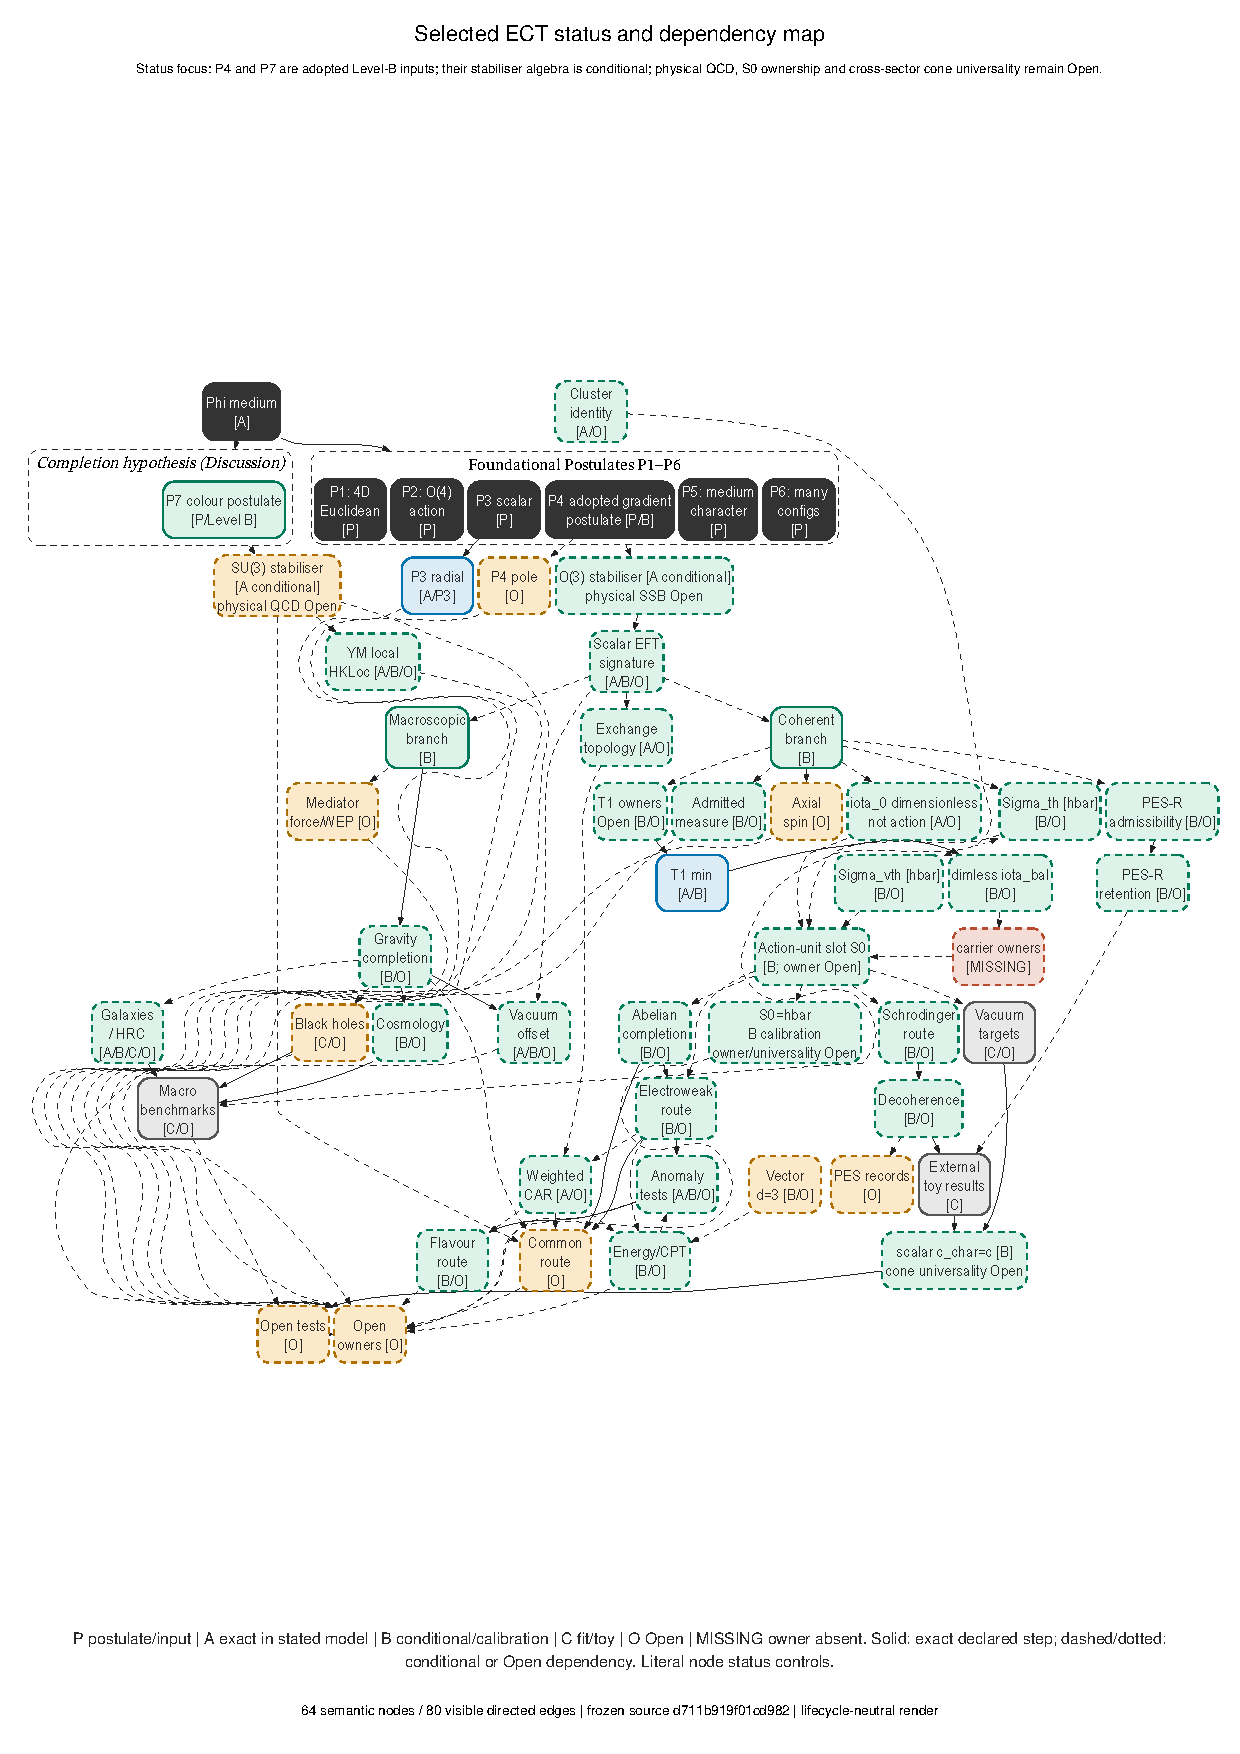
\includepdf[
  pages=1,
  fitpaper=true,
  pagecommand={\thispagestyle{empty}}
]{../figures/r185/logic_maps/whole_status_dependency.pdf}
\clearpage

\section{Open problems of physics addressed within ECT}

Within its framework, ECT addresses several well-known open problems of modern physics:

\begin{enumerate}
\item \textbf{Quantum--gravity completion programme.} Quantum/open-system structures and a scalar characteristic geometry share the ordered-medium architecture, but a physical tensor, universal metric and gravitational record channel remain Open.

\item \textbf{The origin of time.} Within the supplied local algebraic scalar-operator inventory, residual $O(3)$ symmetry fixes the tensor basis; the independently supplied tensor is Lorentzian iff $\beta(\beta-\alpha)<0$; on the retained $\beta>0$ component this is $\alpha>\beta>0$ (A-math conditional). P4/SSB does not select those coefficients or derive the physical clock/universal metric (Open).

\item \textbf{The dark matter problem.} No dark-matter particle candidate has been established in direct, indirect or collider searches.  The HRC-only algebraic diagnostic models the galactic mass-discrepancy channel without a particle-halo term (\emph{C}); its source/force map is not derived, and this does not exclude hidden-sector particles.

\item \textbf{The cosmological constant problem.}  ECT currently
supplies an exact fixed-determinant orientation identity, not an unconditional
vacuum-decoupling theorem.  A separately supplied trace-free scalar--tensor
completion is classically shift covariant through $V+C_I$, and a distinct
two-slope completion supplies a regular late-de-Sitter proof of class.  The
derivation of either physical completion from the $\Phi$ medium, its
radiative protection, universal metric and cosmological state remains Open.

\item \textbf{The Hubble tension.} ECT does not yet own a numerical shift: a complete recombination-to-distance-ladder pipeline from one action and state is Open.

\item \textbf{JWST early galaxies.} A quantitative abundance and morphology prediction requires the full ECT background, perturbation, halo, baryonic and selection forward model; this remains Open.

\item \textbf{Baryon asymmetry.} Only an external observational target and a
missing-owner inventory are available; the physical baryon current/violating
vertex, nonzero CP source and state, transition, transport, washout and
ECT-native derivation remain Open.

\item \textbf{Black-hole information paradox.} A thermal marginal is compatible with global purity under a separately supplied Hilbert-space split and isometry.  Global ECT unitarity, a physical shell, Page curve and constructive evaporation solution remain Open; the shell/Page toys are Level~C/Open.

\item \textbf{The measurement problem.} A specified reduced-sector decoherence model can suppress interference, but PES-R supplies no Born or measurement derivation. Exact weights, pointer-basis selection, single outcome, and the update theorem remain Open.

\item \textbf{The origin of quantum mechanics.} For supplied Gaussian/free Euclidean kernels satisfying the complete applicable corrected OS-II package, the quotient-and-completion construction gives a conditional Hilbert-space route.  Extending it to the interacting $\Phi$ theory and identifying the physical observables, time/metric and state remain Open.  Ordinary projector Gleason applies only at complex dimension at least three with the full supplied measure hypotheses; a qubit requires a supplied Busch effect/POVM or named extension.  Neither route originates probability, a unique outcome or an update rule.

\item \textbf{The arrow of time.} P4 supplies a Euclidean orientation.  Retarded orientation exists only in a supplied hyperbolic scalar problem after an initial--boundary choice; it is not a physical or thermodynamic arrow.  Neither retardedness nor positive pairwise dephasing fixes the sign of von Neumann entropy.  An ECT-specific second-law theorem remains Open pending the reduced map, state or fixed point, entropy functional and detailed-balance/contractivity hypotheses.

\item \textbf{The need for inflation.} ECT organises structural or conditional
non-inflationary routes to horizon-scale homogeneity and a flat baseline branch.
The supplied $S^3$ orientation target has $\pi_2=0$, but its identification
with the complete cosmological vacuum manifold and a physical relic conclusion
remain Open. A supplied pure-quartic ordering kernel gives
an exact flat formal local seed, but the physical band, state, transfer,
branch-selection probability and full observed spectrum remain Open; the
analysis does not establish that inflation is phenomenologically unnecessary.

\item \textbf{The hierarchy problem.} For the displayed matched scales,
$M_{\rm Pl}/M_{\rm EW}\sim10^{16}$ and
$\mathcal I_{\rm EW}=\ln(\phi_0/v_2)\approx36.8$.  These are external/input
arithmetic, not an ECT solution or a scale-generation prediction.  Four
candidate templates remain possible (asymptotic-freedom-like running,
walking/near-conformal dynamics, Miransky/BKT scaling, and
topological/Hopf-like routes). This is a reduction, not a solution: the
broader programme decomposes into OP-EW-scale, OP-EW-locking, OP-EW-gauge,
OP-EW-naturalness, and OP-EW-matter. The first-principles dynamics and the
full electroweak completion remain open (\emph{B/Open}).

\item \textbf{Why a $3+1$ split, and what follows for exchange topology?} Given P1 and the supplied P4 vector chart, one coordinate is an aligned temporal seed and three are transverse; its physical realisation and the deeper origin of four-dimensionality remain Open/OP0.  For two supplied identical point excitations in the exact defect-free domain $\mathcal M_2=((\mathbb R^3\times\mathbb R^3)\setminus\Delta)/S_2$, $\pi_1(\mathcal M_2)=\mathbb Z_2$, so the continuous Abelian braid phases characteristic of two-dimensional anyons are unavailable.  Bosonic/fermionic characters require an additional one-dimensional representation choice; representation selection, higher-dimensional $S_N$ sectors, CAR and spin--statistics remain Open (\emph{A topology conditional on the supplied domain / Open physical statistics}).

\item \textbf{What does the supplied $S^3$ target say about monopoles?} $\pi_2(S^3)=0$, so maps into that target have no $\pi_2$ charge (A-math conditional).  The complete physical vacuum/configuration space, transition owner and relic-production history remain Open, so this is not yet a physical ECT monopole anti-prediction.  Later gauge-completion sectors have separate topology and abundance owners.

\item \textbf{Amplitude-potential stability.} In the homogeneous P3 amplitude sector, the minima $\Phi=\pm\phi_0$ are locally stable at tree level, and the standard one-loop scalar running closes the Standard-Model-type high-field metastability channel inside that declared amplitude closure: here $\beta_\lambda>0$, unlike the Higgs sector of the Standard Model where the top-Yukawa contribution drives metastability. The symmetric point $\Phi=0$ is a hilltop, not a metastable minimum, so Coleman false-vacuum decay does not apply to the minimal P3 potential. None of this proves stationarity or stability of the P4 gradient chart; the complete ordered-state action/Hessian and any secondary electroweak inheritance remain Open (\emph{B/Open}).

\emph{Vacuum decay as a conditional Euclidean benchmark.} The Coleman bounce is standard semiclassical mathematics only after a Lorentzian quantum theory, analytic continuation, contour/thimble, measure, state, boundary data, clock and fluctuation determinant are supplied.  Bare Euclidean DP alone does not assign a transition amplitude or decay rate.  ECT may compare a future completed coherent sector with that benchmark, but currently supplies no distinct decay owner.  For the minimal primary condensate potential, the false-vacuum structure required by Coleman decay is absent.

\item \textbf{Quantum gravity.} The shared-medium architecture motivates a completion programme, but the physical tensor, source, canonical scale and record channel are not derived (\emph{Open}).

\item \textbf{Cosmological coincidence question.} ECT does not yet derive $\Omega_m$, the physical late-time source, or their evolution; the question remains Open.

\item \textbf{Physical spin-2 sector.} The fixed map has no linear TT/static-density seed only at fixed $\alpha,\beta$, about homogeneous $\bar n=w$, and at tangent-director order; quadratic/nonlinear/composite routes remain parametric/Open.  A massless Fierz--Pauli action is an Open completion target, and the LIGO mass bound is an external gate for that target.


\item \textbf{Are $c$, $G_N$, and $\hbar$ already unified?} No.  The scalar coefficients fix only $\hat c_*$; $c_{\rm char}=c_{\rm u}\hat c_*/\mathcal N_\Phi$ uses the clock map, while $c_{\rm char}=c$ and $S_0=\hbar$ are separately adopted Level-B calibrations.  $G_N^{\rm nat}=(8\pi M_G^2)^{-1}$ is a separate tensor matching, and photon/tensor cone equality plus the microscopic origin and universality of the calibrations remain Open.

\item \textbf{Can Casimir, Unruh, Hawking, and particle-production effects belong to one family?} ECT poses this as an Open common-response programme.  Their displayed calculations currently use different supplied bundles, states, boundaries, detectors and geometries.

\item \textbf{Why can a smooth positive kinetic weight not by itself weaken
Pauli exclusion in the supplied local CAR model?} In a separately supplied
local first-order fermionic/CAR EFT, an invertible canonical normalisation
removes a smooth strictly positive temporal kinetic factor while preserving
the supplied CAR algebra.  This excludes Pauli violation generated solely by
that factor.  It does not cover singular or sign-changing factors, nonlocal
branch mixing, defects/coherence loss, or an altered symplectic/CAR structure
(\emph{Level-A conditional mathematics / Open physical ECT}).

\item \textbf{Fine-structure constant.} The standard identities and external
one-loop running may be used as checks after a photon, charge normalisation,
matter representations and matching scale are supplied.  ECT currently
derives none of those physical owners and therefore predicts no value of
$\alpha_{\rm fs}$ (\emph{Open ECT}).

\item \textbf{$S_8$ / lensing--growth sector.}
A future covariant $S_n[g,n,\lambda_n]$ could define an orientation
contribution to the weak-lensing/growth sector.  At present the functions
$\mu(k,z)$, $\eta(k,z)$, and $\Sigma(k,z)$ are explored only with external
proxies; no ECT orientation stress or $S_8$ correction is derived
(\emph{Level~C/Open}).
\end{enumerate}

The technical preprint provides a broad status table comparing about seventy
structures---some postulated, some derived within standard frameworks, and
some empirical inputs---with ECT's classifications as conditional
mathematics, reconstruction targets, supplied diagnostics or Open problems.
A complementary mixed-status table records candidate-completion tests,
benchmarks and Open observational handles; only a completed row with its own
action, state, observable and uncertainty model can become an ECT-specific
prediction.


\section{Conclusion}

ECT is an attempt to place spacetime, gravity, and quantum behaviour within a single pre-spacetime framework. In its current form, some parts of this programme are structural results, some are closure-dependent effective constructions, and some remain open.

\textbf{Common pre-geometric architecture of interactions.}
ECT organises a conditional Abelian route, a candidate weak-sector route and a colour programme in one framework. For colour, $\dim\mathfrak{su}(3)>\dim\mathfrak{so}(4)$ excludes only a direct injective embedding in the displayed minimal algebra; emergent/nonlinear, reducible/singlet, independently supplied bundle and defect-kernel routes remain possible. P7 is an adopted positive-definite Hermitian rank-three bundle postulate with fibrewise $SU(3)$ reduction (Level-B input / Level-A conditional reduction), not a necessary or unique physical gauge completion; its physical-colour map remains Open. Together with the Open gravity completion and generic director coupling this remains an architecture, not a unification theorem. Physical $U(1)_{\rm em}$, photon, colour connection/action, gauge quotient/reduced Hessian, charges, matter representations, anomaly cancellation and the Weinberg angle remain Open.

\textbf{Discrete-symmetry architecture.}
ECT identifies exact Euclidean reflection identities and a conditional route to physical discrete symmetries.  Interpreting those reflections as parity or time reversal requires clock, rod and matter maps; OS/CPT reconstruction is controlled only in supplied free/quadratic local sectors and remains Open for the full nonlinear theory.  The preferred-direction vector operator has a standard conditional discrete-symmetry classification, but its nonzero coefficient and physical matter owner are Open.  It does not change representation-data anomaly coefficients and it does not supply the missing chiral gauge sector.

\textbf{Flavour architecture.}
The observed ``CKM small, PMNS large'' dichotomy can be represented in a
supplied overlap-plus-seesaw flavour model: quark and charged-lepton Yukawa
matrices and the neutrino seesaw matrix may have different basis
misalignments.  ECT has not derived those matrices, their complex phases, or
the preferred-direction flavour operator, so neither the dichotomy nor
leading PMNS/MSW propagation is presently an ECT prediction.  Mixing angles,
CP and Majorana phases, and the absolute spectrum remain Open.

\textbf{What is established or supplied at the strongest declared level:}
the P4 direction is a supplied datum whose $O(3)$ stabiliser is exact group
mathematics, while its physical state and selection remain Open; the conditional Lorentzian
classification of a scalar principal tensor for independently supplied
$\beta(\beta-\alpha)<0$; one scalar characteristic cone with physical gauge, fermion
and tensor cones Open; a status-separated equation inventory: Euclidean scalar boundary problem, supplied KG-form scalar equation, and separately supplied complex Schr\"odinger sector whose conditional NR relation does not prove common descent; retarded support for declared hyperbolic scalar
operators; and generic reduced-state identities with global ECT unitarity
Open.

\textbf{What is conditional or model-internal:}
the BTFR slope exactly~4 after a separate galactic gravity bridge; selected background diagnostics; and C/Open shell/Page toys that do not derive black-hole entropy or evaporation.

\textbf{What is obtained at effective, fit, or closure level (mixed B/C/Open):}
Newton's constant, Planck's constant, and $c$ enter through declared matching
relations.  The primary-amplitude one-loop stability result and the scalar-only
metric equation hold inside their stated ansatzes; a covariant orientation
stress remains Open.  The named two-slope action and state supply a
conditional background diagnostic, not a P1--P6 prediction.  The 165-galaxy HRC-only SPARC registry has absolute held-out $\chi^2/{\rm point}$ of order $30$ (Level~C stress diagnostic); its scalar/ECT source map and any $\Xi$ law are Open.  Decoherence,
PES retains a B/Open ceiling; physical black-hole area scaling is Open,
while Page-curve-like shell behaviour and the shell itself are C/Open.  The
boundary-sensitive Casimir response remains Open ECT;
the exact black-hole coefficient and a constructive Page curve are Open.

\textbf{What remains an open programme:}
Three fermion generations; Yukawa hierarchy; $\alpha = 1/137$; renormalisability; Born rule as first-principles theorem; Bell correlators; complete BH evaporation; gradient condensation from bare P3; proton stability as a UV discriminant (three selection-rule patterns conditional on gauge/flavour completion). This also includes the full interacting closure of the conditional CPT route, the exact derivation of the maximally parity-violating weak-sector pattern, and the flavour-architecture derivation targets (CKM and PMNS mixing parameters, CP phases, absolute neutrino spectrum) under OP-Yukawa. The constancy of the dimensionless constants $\alpha$ and $\mu$ is recorded only as a conditional selective-coupling protection route (OP-CONST); the unconditional microscopic proof remains open and belongs to OP-matter plus OP-grad completion.

\textbf{Status-separated architectural summary.}
The ordered-medium framework supplies candidate reconstructions and common
organising language, with explicit status ceilings.  The effective-metric
route, excitation classification, coherent-sector reconstruction programme,
and reduced-record description are not all theorem-level outputs.  In
particular, coherent interactions can exchange energy/momentum and entangle;
decoherence is required only for irreversible record formation in a specified
reduced model.  The $70.6\,\mathrm{ms}$ sphere point is external conditional
arithmetic, not a Diósi--Penrose/environment crossover or ECT rate: the
physical ECT projector, vertex, state/noise kernel, normalisation and apparatus
protocol remain Open, and recoherence remains protocol dependent.

\small
\renewcommand{\arraystretch}{1.12}
\begin{longtable}{@{}p{3.0cm}p{7.0cm}p{2.0cm}p{2.0cm}@{}}
\caption{Status-separated ECT architecture and foundational questions.}
\label{tab:pop_distinctive}\\
\toprule
Item & Current ECT statement & Status & Scope \\
\midrule
\endfirsthead
\multicolumn{4}{c}{\tablename\ \thetable\ (continued)}\\
\toprule
Item & Current ECT statement & Status & Scope \\
\midrule
\endhead
\midrule
\multicolumn{4}{r}{Continued on next page}\\
\endfoot
\bottomrule
\endlastfoot
Effective-metric route & Ordered-branch construction inside declared scalar/orientation programmes; complete covariant gravity and physical orientation stress remain Open & B/Open & Architectural \\
Excitation sectors & Scalar, gauge-candidate, orientation, and topological sectors form a status-separated classification; full Standard-Model matter content is not derived & A/B/Open & Classification \\
Quantum reconstruction & Quadratic RP/OS and wave-kinematic routes are controlled; Born, pointer basis, single outcome, and interacting completion remain conditional/Open & A-math/B/Open & Programme \\
Coherent coupling and records & Coherent coupling can exchange energy/momentum and entangle; traced uncontrolled channels generate irreversible records in specified reduced models & B/Open & No universal threshold \\
Fock-space route & Variable excitation number is a reconstruction target, not a foundational ECT theorem & Open & Conceptual \\
Why a $3+1$ split? & Given P1 and the supplied P4 vector chart, one aligned coordinate and three transverse coordinates are identified; physical realisation and the origin of four dimensions remain Open/OP0 & A-math conditional / Open physical & Structural \\
Primary monopole topology & $\pi_2(S^3)=0$ for the supplied orientation target; physical vacuum-manifold identification, transition and relic conclusion remain Open & A-math conditional / Open physical & Target-space limited \\
Amplitude-potential stability & Tree/local and primary-amplitude one-loop checks hold in their declared P3 closures; P4 gradient-state and global/metastable completion remain Open & B/Open & Closure limited \\
Quantum gravity & A common-medium architecture reframes the relation; UV, spin-2 RP/OS, and interacting closure remain Open & B/Open & Architectural \\
Physical spin-2 route & No linear TT/static-density seed only at fixed $\alpha,\beta$, homogeneous $\bar n=w$ and tangent-director order; quadratic/nonlinear routes, constrained action, source and TT projection Open & A-math conditional negative result / Open physical completion & Completion target \\
Gravitational record channel & The $51/160$, $70.6\,\mathrm{ms}$ hard-sphere point and the unit-coefficient guide/crossover relations are distinct external comparisons; none supplies an ECT projector, vertex, state/noise kernel or absolute rate & External A/C; ECT Open & Not ECT-specific \\
Recoherence & Echo/control recovery is protocol dependent; no universal forward/reverse probability law is derived & Open & Protocol specific \\
Late-time source & Conditional scalar proof-of-class; physical source and $w(a)$ Open & Open & Owner programme \\
Director spin/WEP completion & Homogeneous vector term has no spin splitting and no source-generated force; spin-dependent operator and body-force owners are absent & B operator classification / Open observables & External constraints only \\
\end{longtable}
\normalsize

ECT places the galactic mass-discrepancy, late-time background and quantum-reconstruction programmes within one medium architecture.  This does not eliminate their independent closure data: the HRC gravity bridge and particle content, the selected cosmological action/state, and the quantum state/operator/probability owners remain B/C/Open.  No reduced bare-parameter count is claimed until these owners and their matching constants have been derived.

Whether ECT ultimately becomes a viable theory of nature or remains a productive conceptual laboratory, it does something valuable: it shows how spacetime, gravitational response, and quantum-theoretic structure can be placed within a common condensate architecture, with some parts derived, others reconstructed, and others left as explicit closure targets. It identifies the specific structures --- gradient condensation, compact-phase topology, orientation stiffness, and the Principle of Euclidean Stationarity --- that make this unification programme possible.

Inside a supplied ordered scalar branch, the programme conditionally models a distinguished direction and scalar propagation structure. Whether this becomes physical time requires the clock, metric, matter and branch-selection maps, which remain Open. Thus the idea that the universe forms time is a conditional programme hypothesis, not a P1--P6 derivation.

\paragraph{Reference scope.}
The numerical values and observational targets quoted in this companion are
external comparison data, not evidence for ECT.  Displayed digits are
deterministic rounding of the stated arithmetic at declared inputs and
conventions, not uncertainty statements or physical precision; inference
requires input covariances and an owner-complete action/state-to-observable or
likelihood chain.  The principal source owners
are GW170817 for the tensor-speed gate~\cite{LIGO_Virgo_GW170817_2017},
Planck for the reference cosmology~\cite{Planck2018}, SH0ES for the local
Hubble calibration~\cite{Riess2022}, DESI analyses for late-time distance
constraints~\cite{DESIDR2_2025,Lodha2025}, JWST studies for early-galaxy
targets~\cite{Bunker2023,Carniani2024}, SPARC/RAR data for rotation-curve
comparisons~\cite{Lelli2016,McGaugh2016}, and MICROSCOPE for the
equivalence-principle gate~\cite{MICROSCOPE2022}.  Every ECT interpretation
retains the A/B/C/Open status assigned in the preprint.

\renewcommand{\refname}{Selected references and data sources}
\addcontentsline{toc}{section}{Selected references and data sources}
\bibliographystyle{unsrt}
\bibliography{references}

\vspace{2em}
\noindent\rule{\textwidth}{0.5pt}

\noindent\textbf{Note.}
This article is a narrative companion to:
\emph{``Euclidean Condensate Theory (ECT): Conditional Routes from a
Euclidean Condensate to Lorentzian Kinematics, Quantum Structures, and
Gravity''} by Valeriy Blagovidov (2026).

\medskip
\noindent
Preprint Zenodo concept DOI:
\href{https://doi.org/10.5281/zenodo.18917929}{doi:10.5281/zenodo.18917929}.

\medskip
\begin{center}
\url{https://github.com/chufelo/ECT-preprint-code}\\[0.75em]
Companion Zenodo concept DOI:\\
\url{https://doi.org/10.5281/zenodo.19430795}
\end{center}

\end{document}
